% Este documento tem a ver com as partes do LIVRO. 

% Tamanhos
% \tiny
% \scriptsize
% \footnotesize
% \small 
% \normalsize
% \large 
% \Large 
% \LARGE 
% \huge
% \Huge

% Posicionamento
% \centering 
% \raggedright
% \raggedleft
% \vfill 
% \hfill 
% \vspace{Xcm}   % Colocar * caso esteja no começo de uma página. Ex: \vspace*{...}
% \hspace{Xcm}

% Estilo de página
% \thispagestyle{<<nosso>>}
% \thispagestyle{empty}
% \thispagestyle{plain}  (só número, sem cabeço)
% https://www.overleaf.com/learn/latex/Headers_and_footers

% Compilador que permite usar fonte de sistema: xelatex, lualatex
% Compilador que não permite usar fonte de sistema: latex, pdflatex

% Definindo fontes
% \setmainfont{Times New Roman}  % Todo o texto
% \newfontfamily\avenir{Avenir}  % Contexto

\begingroup\thispagestyle{empty}

\begin{textblock*}{2.625in}(0pt,0pt)%
\vspace*{-3.5cm}
%\hspace*{-4cm}
\includegraphics[scale=1]{../watermarks/front5ano.pdf}
\end{textblock*}
                
              \vspace*{\fill}
              \begin{center}
              {\HUGE\textbf{Revisa SAEB}}\bigskip

              {\LARGE\textbf{2º ano: Matemática}}

              \bigskip
              \bigskip
              \bigskip

              {\Large
                            AUTORIA

                            }
              \end{center}
              \vspace*{\fill}

\endgroup
\pagebreak       % [Frontistício]
%\newcommand{\linhalayout}[2]{{\tiny\textbf{#1}\quad#2\par}}
\newcommand{\linha}[2]{\ifdef{#2}{\linhalayout{#1}{#2}}{}}

\begingroup\tiny
\parindent=0cm
\thispagestyle{empty}

\textbf{Gerência editorial}\quad			 {Ana Mortara}\\
\textbf{Assistência editorial}\quad			 {Paula Dias}\\
\textbf{Assistência administrativa editorial}\quad {Gisele Cerchiaro}\\

\hspace{-5pt}\begin{tabular}{ll}
\textbf{Elaboração de conteúdo} & Abraão Augusto (Língua Portuguesa),	\\
								& Alessandra Domingues Juliano (Língua Portuguesa),	\\
								& Ana Paula Souza Rios (Língua Portuguesa),	\\
								& André Sanchez Astorino (Língua Portuguesa e Língua Inglesa),	\\
								& Clarissa Ayres Mendes (Língua Portuguesa),	\\
								& Eduardo Toniolo Campos (Matemática),	\\
								& Fernanda Dobashi (Língua Portuguesa),	\\
								& Guilherme Salles (Ciências Humanas),	\\
								& Letícia Leme (Ciências Humanas),	\\
								& Lucas Della Santina (Educação Física),	\\
								& Pilar Espí (Arte),	\\
								& Renata Cândido Carvalho (Ciências da Natureza),	\\
								& Thiago Figueiredo (Matemática),	\\
								& Victor Marques (Ciências da Natureza)	\\
\end{tabular}


\textbf{Edição}\quad	 {Carlos Rogério Duarte Barreiros, Fábia Alvim, Felipe Augusto Neves Silva}\\
\textbf{Preparação e revisão}\quad			 {Saíra Editorial}\\
\textbf{Coordenação de arte}\quad			 {Jorge Sallum}\\
\textbf{Editoração eletrônica}\quad			 {Paulo Henrique Pompermaier}\\
\textbf{Pesquisa iconográfica}\quad			 {Margarita Veloso}\\
\textbf{Projeto gráfico e capa}\quad		 {Luísa Marcelino}\\
\textbf{Código}\quad {\ifdef{\RevisionInfo{}}{\RevisionInfo{} (\today, \currenttime)}{001}\medskip}

\noindent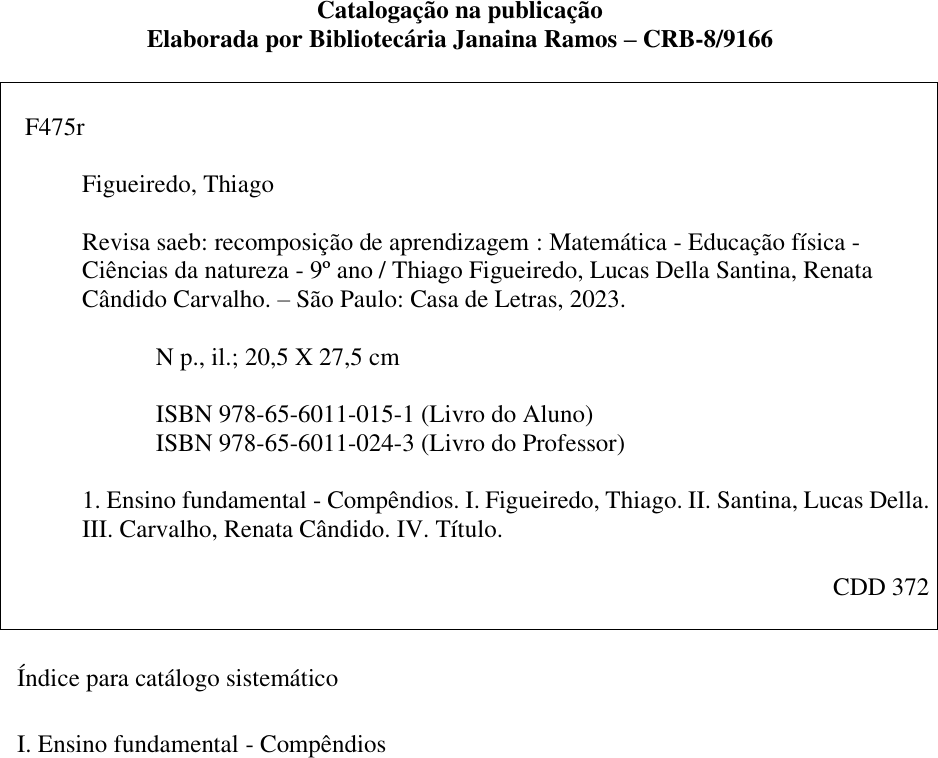
\includegraphics[width=.5\textwidth]{../fichas/9MAT.png}

\vfill

\textsc{casa de letras e gráfica ltda.}\\
Rua Fradique Coutinho, 1139, andar 2, sala 2\\
CEP 05416--011 -- São Paulo/\textsc{sp}, Brasil\\
Telefone: (11) 3914--7790\\\smallskip
www.casadeletras.com.br\\

\endgroup
\pagebreak
     % [Créditos]
% nothing			is level -3
% \book				is level -2
% \part				is level -1
% \chapter 			is level 0
% \section 			is level 1
% \subsection 		is level 2
% \subsubsection 	is level 3
% \paragraph 		is level 4
% \subparagraph 	is level 5
\setcounter{secnumdepth}{2}
\setcounter{tocdepth}{0}
 
% \renewcommand{\contentsname}{Índex} 	% Trocar nome do sumário para 'Índex'
%\ifodd\thepage\relax\else\blankpage\fi 	% Verifica se página é par e coloca página branca
%\tableofcontents*

\pagebreak
{\begingroup\mbox{}\pagestyle{empty}
\pagestyle{empty} 
% \renewcommand{\contentsname}{Índex} 	% Trocar nome do sumário para 'Índex'
%\ifodd\thepage\relax\else\blankpage\fi 	% Verifica se página é par e coloca página branca
\addtocontents{toc}{\protect\thispagestyle{empty}}
\addtocontents{toc}{\vspace*{-1cm}}
\tableofcontents*\clearpage\endgroup}

%\newwatermark[pagex={4}]{\vspace{2.5cm}\hspace*{7.8cm}
\includegraphics[scale=1]{../watermarks/intro5ano.pdf}}

\newwatermark[pagex={6,142,166}]{\vspace{2.5cm}\hspace*{7.8cm}
\includegraphics[scale=1]{../watermarks/1modulo5ano.pdf}}
\newwatermark[pagex={16,148}]{\vspace{2.5cm}\hspace*{7.8cm}
\includegraphics[scale=1]{../watermarks/2modulo5ano.pdf}}
\newwatermark[pagex={175}]{\vspace{2.5cm}\hspace*{7.8cm}
\includegraphics[scale=1]{../watermarks/2modulo5ano_impar.pdf}}
\newwatermark[pagex={24}]{\vspace{2.5cm}\hspace*{7.8cm}
\includegraphics[scale=1]{../watermarks/3modulo5ano.pdf}}
\newwatermark[pagex={155,185}]{\vspace{2.5cm}\hspace*{7.8cm}
\includegraphics[scale=1]{../watermarks/3modulo5ano_impar.pdf}}
\newwatermark[pagex={32}]{\vspace{2.5cm}\hspace*{7.8cm}
\includegraphics[scale=1]{../watermarks/4modulo5ano.pdf}}
\newwatermark[pagex={39}]{\vspace{2.5cm}\hspace*{7.8cm}
\includegraphics[scale=1]{../watermarks/5modulo5ano_impar.pdf}}
\newwatermark[pagex={50}]{\vspace{2.5cm}\hspace*{7.8cm}
\includegraphics[scale=1]{../watermarks/6modulo5ano.pdf}}
\newwatermark[pagex={59}]{\vspace{2.5cm}\hspace*{7.8cm}
\includegraphics[scale=1]{../watermarks/7modulo5ano_impar.pdf}}
\newwatermark[pagex={65}]{\vspace{2.5cm}\hspace*{7.8cm}
\includegraphics[scale=1]{../watermarks/8modulo5ano_impar.pdf}}
\newwatermark[pagex={78}]{\vspace{2.5cm}\hspace*{7.8cm}
\includegraphics[scale=1]{../watermarks/9modulo5ano.pdf}}
\newwatermark[pagex={88}]{\vspace{2.5cm}\hspace*{7.8cm}
\includegraphics[scale=1]{../watermarks/10modulo5ano.pdf}}
\newwatermark[pagex={95}]{\vspace{2.5cm}\hspace*{7.8cm}
\includegraphics[scale=1]{../watermarks/11modulo5ano_impar.pdf}}
\newwatermark[pagex={102}]{\vspace{2.5cm}\hspace*{7.8cm}
\includegraphics[scale=1]{../watermarks/12modulo5ano.pdf}}
\newwatermark[pagex={111}]{\vspace{2.5cm}\hspace*{7.8cm}
\includegraphics[scale=1]{../watermarks/13modulo5ano_impar.pdf}}
\newwatermark[pagex={119}]{\vspace{2.5cm}\hspace*{7.8cm}
\includegraphics[scale=1]{../watermarks/14modulo5ano_impar.pdf}}
\newwatermark[pagex={127}]{\vspace{2.5cm}\hspace*{7.8cm}
\includegraphics[scale=1]{../watermarks/15modulo5ano_impar.pdf}}

\newwatermark[pagex={5,7,9,11,13,15,17,19,21,23,25,27,29,31,33,35,37,39,41,43,45,47,49,51,53,55,57,59,61,63,65,67,69,71,73,75,77,79,81,83,85,87,89,91,93,95,97,99,101,103,105,107,109,111,113,115,117,119,121,123,125,127,129,131,133,135,137,139,143,145,147,149,151,153,155,157,159,161,167,169,171,173,175,177,179,181,183,185,187,189,191}]{\vspace{2.5cm}\hspace*{8cm}
\includegraphics[scale=1]{../watermarks/bg5anoimpar.pdf}}

\newwatermark[pagex={8,10,12,14,16,18,20,22,26,28,30,32,34,36,38,40,42,44,46,48,50,52,54,56,58,60,62,64,66,68,70,72,74,76,78,80,82,84,86,88,90,92,94,96,98,100,102,104,106,108,110,112,114,116,118,120,122,124,126,128,130,132,134,136,138,144,146,148,150,152,154,156,158,160,162,168,170,172,174,176,178,180,182,184,186,188,190,192}]{\vspace{2.5cm}\hspace*{7.8cm}
\includegraphics[scale=1]{../watermarks/bg5anopar.pdf}}

\newwatermark[pagex={195,197,199,201,203,207,209,211,213,215,219,221,223,225,227,231,233,235,237,239,241,243}]{\vspace{2.5cm}\hspace*{8cm}
\includegraphics[scale=1]{../watermarks/bgsim5anoimpar.pdf}}

\newwatermark[pagex={194,196,198,200,202,204,206,208,210,212,214,218,220,222,224,226,228,230,232,234,236,238,240,242,244}]{\vspace{2.5cm}\hspace*{7.8cm}
\includegraphics[scale=1]{../watermarks/bgsim5anopar.pdf}}

%!TEX root=./LIVRO.tex
\chapter{APRESENTAÇÃO}

O \textbf{SISTEMA DE AVALIAÇÃO DA EDUCAÇÃO BÁSICA (SAEB)} É UM CONJUNTO
DE AVALIAÇÕES EXTERNAS EM LARGA ESCALA QUE PERMITE AO INSTITUTO NACIONAL
DE ESTUDOS E PESQUISAS EDUCACIONAIS ANÍSIO TEIXEIRA (INEP) REALIZAR UM
DIAGNÓSTICO DA EDUCAÇÃO BÁSICA BRASILEIRA E DE FATORES QUE PODEM
INTERFERIR NO DESEMPENHO DOS ESTUDANTES.

POR MEIO DE TESTES E QUESTIONÁRIOS, APLICADOS A CADA DOIS ANOS NA REDE
PÚBLICA E EM UMA AMOSTRA DA REDE PRIVADA, O SAEB REFLETE OS NÍVEIS DE
APRENDIZAGEM DEMONSTRADOS PELOS ESTUDANTES AVALIADOS, EXPLICANDO ESSES
RESULTADOS A PARTIR DE UMA SÉRIE DE INFORMAÇÕES CONTEXTUAIS.

O SAEB PERMITE QUE AS ESCOLAS E AS REDES MUNICIPAIS E ESTADUAIS DE
ENSINO AVALIEM A QUALIDADE DA EDUCAÇÃO OFERECIDA AOS ESTUDANTES. O
RESULTADO DA AVALIAÇÃO É UM INDICATIVO DA QUALIDADE DO ENSINO BRASILEIRO
E OFERECE SUBSÍDIOS PARA ELABORAÇÃO, MONITORAMENTO E APRIMORAMENTO DE
POLÍTICAS EDUCACIONAIS, SEMPRE COM BASE EM EVIDÊNCIAS.

AS MÉDIAS DE DESEMPENHO DOS ESTUDANTES, APURADAS NO SAEB, JUNTAMENTE COM
AS TAXAS DE APROVAÇÃO, REPROVAÇÃO E ABANDONO, APURADAS NO CENSO ESCOLAR,
COMPÕEM O ÍNDICE DE DESENVOLVIMENTO DA EDUCAÇÃO BÁSICA (IDEB).

REALIZADO DESDE 1990, O SAEB PASSOU POR UMA SÉRIE DE APRIMORAMENTOS
TEÓRICO-METODOLÓGICOS AO LONGO DAS EDIÇÕES. A EDIÇÃO DE 2019 MARCA O
INÍCIO DE UM PERÍODO DE TRANSIÇÃO ENTRE AS MATRIZES DE REFERÊNCIA
UTILIZADAS DESDE 2001 E AS NOVAS MATRIZES ELABORADAS EM CONFORMIDADE COM
A BASE NACIONAL COMUM CURRICULAR (BNCC).

\section*{REVISA SAEB: REFORÇO ESCOLAR}

COMO O PRÓPRIO NOME DIZ, A EDUCAÇÃO BÁSICA É AQUELA EM QUE SE PROMOVE A
FORMAÇÃO MAIS ESSENCIAL DOS ALUNOS. O SISTEMA DE AVALIAÇÃO DA EDUCAÇÃO
BÁSICA (SAEB) AJUDA NA DETECÇÃO DOS PONTOS FORTES E FRACOS NA FORMAÇÃO
DOS ALUNOS EM ESTADOS, EM MUNICÍPIOS, EM ESCOLAS, FUNCIONANDO COMO UM
PARÂMETRO PARA QUE PROBLEMAS SEJAM SOLUCIONADOS E PARA QUE, ANO APÓS
ANO, ESSA FORMAÇÃO EVOLUA E AJUDE NO CRESCIMENTO DESSAS ESCOLAS, DESSES
MUNICÍPIOS E DESSES ESTADOS.

A PREPARAÇÃO ADEQUADA PARA AVALIAÇÕES EM LARGA ESCALA, COMO A DO SAEB, É
IMPORTANTE PARA QUE, NO MOMENTO DA PROVA, OS ALUNOS POSSAM ESTAR ATENTOS
E TRANQUILOS PARA DAREM O MELHOR POSSÍVEL DE SEU POTENCIAL. ASSIM, UM
MATERIAL DIDÁTICO DE APOIO QUE, DE FATO, PROMOVA ESSA PREPARAÇÃO É O
MAIOR DOS ALIADOS PARA PROFESSORES E GESTORES. ESTE MATERIAL TEM
EXATAMENTE ESTA INTENÇÃO: GARANTIR UM MELHOR APROVEITAMENTO DE CADA
ESTUDANTE NA RESOLUÇÃO DE ATIVIDADES, PARA QUE CONSIGAM RESULTADOS
EXCELENTES NESSA TRAJETÓRIA DE AVALIAÇÃO.

O \textbf{REVISA SAEB} ESTÁ DIVIDIDO EM 18 VOLUMES, DISTRIBUÍDOS, AO
LONGO DO ENSINO FUNDAMENTAL, DA SEGUINTE MANEIRA:

\begin{itemize}
\item
  NOS ANOS INICIAIS, PARA O \textbf{PRIMEIRO}, O \textbf{SEGUNDO}, O
  \textbf{TERCEIRO} E O \textbf{QUARTO ANO}, E NOS ANOS FINAIS, PARA O
  \textbf{SEXTO}, O \textbf{SÉTIMO} E O \textbf{OITAVO ANO}, EXISTE UM
  VOLUME POR ANO DE LÍNGUA PORTUGUESA E EXISTE UM VOLUME POR ANO DE
  MATEMÁTICA.
\item
  O \textbf{QUINTO ANO} APRESENTA UMA ESTRUTURA ESPECIAL. EM UM VOLUME,
  APARECEM ESTES COMPONENTES: LÍNGUA PORTUGUESA, ARTE E CIÊNCIAS
  HUMANAS. EM OUTRO VOLUME, APARECEM ESTES COMPONENTES: MATEMÁTICA,
  EDUCAÇÃO FÍSICA E CIÊNCIAS DA NATUREZA.
\item
  O \textbf{NONO ANO} TAMBÉM APRESENTA UMA ESTRUTURA ESPECIAL. SÃO DOIS
  VOLUMES: UM CONTÉM LÍNGUA PORTUGUESA, ARTE, LÍNGUA INGLESA E CIÊNCIAS
  HUMANAS; O OUTRO CONTÉM MATEMÁTICA, EDUCAÇÃO FÍSICA E CIÊNCIAS DA
  NATUREZA.
\end{itemize}

CADA VOLUME, EM CADA COMPONENTE, ESTÁ DIVIDIDO EM MÓDULOS TEMÁTICOS (DE
UMA OU DUAS AULAS), E CADA MÓDULO CONTA COM A ESTRUTURA DESCRITA A
SEGUIR.

\begin{itemize}
\item
  A \textbf{ABERTURA DO MÓDULO} APRESENTA UM RESUMO TEÓRICO DE
  CONTEXTUALIZAÇÃO, VINCULADO, PRINCIPALMENTE, A HABILIDADES DAS
  MATRIZES DO SAEB, MAS TAMBÉM A ALGUMAS HABILIDADES DA BNCC QUE TÊM
  RELAÇÃO COM ESSAS PRIMEIRAS HABILIDADES.
\item
  NA SEQUÊNCIA, ABRE-SE UMA SEÇÃO DE \textbf{ATIVIDADES}, QUE CONTÉM
  EXERCÍCIOS DE MODELOS VARIADOS PARA RETOMADA E FIXAÇÃO
  DO CONTEÚDO TRAZIDO PELO MÓDULO.
\item
  NO FECHAMENTO DE CADA MÓDULO, SURGE UMA SEÇÃO CHAMADA \textbf{TREINO},
  QUE CONTÉM TRÊS ITENS (QUESTÕES NO MODELO DO INEP, QUE É O MESMO
  UTILIZADO NOS TESTES COGNITIVOS DO SAEB). CADA ITEM CHECA O
  DESENVOLVIMENTO DE UMA HABILIDADE DAS MATRIZES DO SAEB E, SEMPRE QUE
  HÁ CONEXÃO, ESTÁ VINCULADO A UMA HABILIDADE DA BNCC DO ANO
  CORRESPONDENTE.
\item
  OS VOLUMES SE ENCERRAM COM QUATRO \textbf{SIMULADOS}, PARA SEREM
  APLICADOS BIMESTRALMENTE. AO LONGO DOS QUATROS SIMULADOS, TODAS AS
  HABILIDADES DAS MATRIZES DO SAEB, EM CADA ANO, SÃO TRABALHADAS, DESDE
  QUE VINCULADAS A CONTEÚDOS PREVISTOS PELA BNCC PARA O ANO EM
  ESPECÍFICO. IGUALMENTE COMPOSTOS DE ITENS, EM NÚMEROS VARIADOS, OS
  SIMULADOS TAMBÉM APRESENTAM, SEMPRE QUE HÁ CONEXÃO, HABILIDADES DA
  BNCC.
\end{itemize}

\addcontentsline{toc}{chapter}{MATEMÁTICA}
%!TEX root=./LIVRO.tex

\chapter{Representações numéricas}


\colorsec{Habilidades do SAEB}

\begin{itemize}
\item
  Escrever números racionais (representação fracionária ou decimal
  finita) em sua representação por algarismos ou em língua materna ou
  associar o registro numérico ao registro em língua materna.
\item
  Compor ou decompor números racionais positivos (representação decimal
  finita) na forma aditiva, ou em suas ordens, ou em adições e
  multiplicações.
\item
  Comparar ou ordenar números reais, com ou sem suporte da reta
  numérica.
\item
  Converter uma representação de um número racional positivo para outra
  representação. 
  \item Identificar um número natural como primo, composto,
  ``múltiplo/\,fator de'' ou ``divisor de'' ou identificar a decomposição
  de um número natural em fatores primos ou relacionar as propriedades
  aritméticas (primo, composto, ``múltiplo/\,fator de'' ou ``divisor de'')
  de um número natural à sua decomposição em fatores primos.
\end{itemize}

\colorsec{Habilidades da BNCC}
\begin{itemize} 
\item EF06MA01
\item EF06MA05
\end{itemize}

\subsection{Classes e ordens numéricas}

%Tabela
\begin{figure}[h]%tpb!]
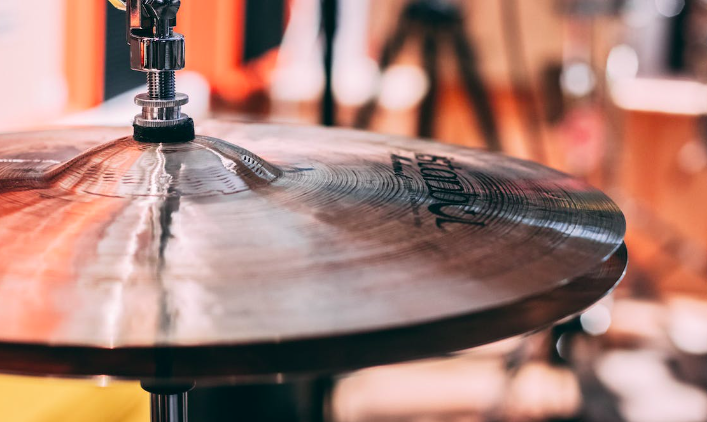
\includegraphics[width=5in,height=2.80208in]{./imgSAEB_6_MAT/media/image1.png}
\end{figure}

\conteudo{
\textbf{Números primos}\quad Considerando o conjunto dos números naturais, definem-se
como números primos aqueles que possuem exatamente dois divisores, o $1$ e
o próprio número em questão. Alguns exemplos de números primos são: $2$,
$3$, $5$, $7$, $11$, $13$ etc.

A decomposição de um número composto em fatores primos consiste em
escrever um número através da multiplicação de números primos que
compõem o próprio número.}

\noindent\textbf{Exemplo:} Decomposição do número $144$ em fatores primos: 

%Tabela
\begin{figure}[htpb!]
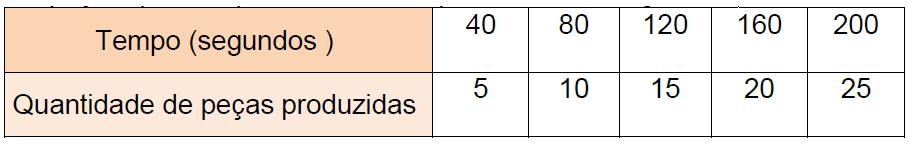
\includegraphics[width=\textwidth]{./imgSAEB_6_MAT/media/image132.png}
\end{figure}

\noindent Veja a seguir \textbf{alguns exemplos} provenientes do sistema de numeração
romano:

% Professor
% \noindent Pedir aos alunos que imaginem um mundo onde os números não existam como
% os conhecemos hoje. Propor que descrevam situações em que é necessário
% utilizarmos números para diferentes finalidades, mas que façam isso sem
% os símbolos que normalmente empregamos. Observar o envolvimento dos
% alunos, motivando-os a compartilhar a opinião com os colegas.

% O objetivo é incentivar o aluno a refletir sobre os números e suas
% diversas utilidades. Provavelmente, ele já possui um conhecimento prévio
% sobre o assunto e utiliza os números em seu cotidiano para contar,
% ordenar, codificar e medir, ao medir sua altura, contar sua idade,
% ordenar seu lugar na fila etc. Propor que os alunos reflitam sobre onde
% eles utilizam os números no cotidiano, desde a hora que acordam até a
% hora de dormir.

\colorsec{Atividades}

\num{1}  Complete abaixo com os números primos entre $2$ e $65$

%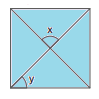
\includegraphics[width=5.47708in,height=1.81389in]{./imgSAEB_6_MAT/media/image10.png}
% Os números primos de $2$ a $65$, que devem ser obtidos pela construção
% proposta aos alunos no boxe, são: $2$, $3$, $5$, $7$, $11$, $13$, $17$, $19$, $23$, $29$, $31$, $37$, $41$, $43$, $47$, $53$, $59$, $61$.

\reduline{Os números primos de $2$ a $65$, que devem ser obtidos pela construção
proposta são: $2$, $3$, $5$, $7$, $11$, $13$, $17$, $19$, $23$, $29$, $31$, $37$, $41$, $43$, $47$, $53$, $59$, $61$.\hfill}\linhas{1}

\num{2}  Indique "V" para as afirmações verdadeiras e "F" para as falsas:

\begin{boxlist}
\boxitem[\rosa{V}] o número $2$ é o único número par que é primo.
\boxitem[\rosa{F}] todos os números ímpares são primos.
\boxitem[\rosa{F}] o número $9$ é primo.
\boxitem[\rosa{V}] o número $121$ possui $3$ divisores.
\boxitem[\rosa{F}] o número $289$ é primo.
\boxitem[\rosa{V}] um número composto possui mais de $2$ divisores.
\boxitem[\rosa{V}] um número primo possui $2$ divisores: o $1$ e ele mesmo.
\boxitem[\rosa{V}] os números $41$, $43$ e $47$ são primos.
\end{boxlist}


\num{3} Decomponha em fatores primos.

\begin{escolha}
\item  $100$    \rosa{$2^2\times 5^2 = 100$}
\item  $60$     \rosa{$2^2\times 3\times 5 = 60$}
\item  $225$    \rosa{$3^2\times 5^2 = 225$}
\item  $1.000$  \rosa{$2^3\times 5^3 = 1.000$}
\item  $36$     \rosa{$2^2\times 3^2 = 36$}
\end{escolha}

\num{4} A decomposição em fatores primos do número $720$ é:

\reduline{$2^4\times 3^2\times 5 = 720$.\hfill}\linhas{1}

\num{5}  O menor número composto formado pelos fatores primos $2$, $3$, $5$ e $11$ é:

\reduline{$2\times 3\times 5\times 11 = 330$.\hfill}\linhas{1}

\num{6}  O número $8$ pode ser fatorado como $8 = 2\times 2\times 2 = 2^3$ e, portanto,
possui $3$ fatores primos. O número $30$ também tem $3$ fatores primos, pois
$30 = 2\times 3\times 5$. Dessa forma, assinale a alternativa que apresenta apenas
números compostos formados por $3$ fatores primos.

\reduline{$25$, $49$, $64$, $81$.\hfill}\linhas{1}

\num{7}  Quais números estão representados abaixo?

% Tabela
\begin{mdframed}[linewidth=2pt,linecolor=azul!20,backgroundcolor=azul!20,roundcorner=2pt]
VIII \hfill XVII \hfill XXIII \hfill LIX \hfill DXLV \hfill MDXCVIII
\end{mdframed}

\reduline{$8$, $17$, $23$. $59$, $545$ e $1598$.\hfill}\linhas{1}

% Professor
%Explorar com eles as regras do sistema de numeração romano nos exemplos
%dos números apresentados na página.

\num{8}  Represente a quantidade de objetos a seguir nos sistemas de numeração
romano e decimal.

\begin{escolha}
\item \reduline{Romano: IX; Decimal: $9$}
\item \reduline{Romano: V; Decimal: $5$}
\item \reduline{Romano: VII; Decimal: $7$}
\end{escolha}

%Tabela
% https://br.freepik.com/fotos-gratis/linha-de-lapis-afiados-verdes-sobre-fundo-branco\_5223660.htm\#query=lined\%20up\%20pencils\&position=21\&from\_view=search\&track=ais.
% Acesso em: 5 maio 2023.

%Tabela
% https://br.freepik.com/fotos-gratis/homem-colheita-segurando-pedido-jogo-livros\_5301939.htm\#query=five\%20books\&position=4\&from\_view=search\&track=ais.
% Acesso em: $5$ maio $2023$.

%Tabela 
% https://br.freepik.com/fotos-gratis/macas-vermelhas-e-verdes-isoladas-na-placa-de-madeira\_14705803.htm\#page=2\&query=twenty\%20apples\&position=30\&from\_view=search\&track=ais

% Professor
% Os números utilizados em jornais em francês, italiano e
% inglês são indo-arábicos. Dessa forma, os alunos terão uma percepção
% concreta da universalidade do sistema de numeração indo-arábico. Uma vez
% que os alunos percebam que o sistema de numeração decimal possui regras
% e características que o fizeram prevalecer sobre os outros sistemas
% apresentados, é chegado o momento de eles verificarem, de fato, quais
% são essas regras e características. Uma estratégia possível é fazer a
% comparação das características do sistema de numeração decimal com
% outros sistemas, ressaltando as diferenças e semelhanças. Com base nessa
% discussão, organizar, com a turma, uma tabela para que os alunos
% sistematizem as regras estudadas de todos os sistemas que foram
% apresentados.

\num{9}  Passe os números do sistema de numeração romano a seguir para o
sistema decimal:

\begin{escolha}
\item IV \reduline{$4$.\hfill}
\item VI \reduline{$6$.\hfill}
\item XL \reduline{$40$.\hfill}
\item LX \reduline{$60$.\hfill}
\item XC \reduline{$90$.\hfill}
\item CX \reduline{$110$.\hfill}
\end{escolha}

\num{10}  O número $35.482$ pode ser decomposto nas parcelas $30.000 + 5.000$ +
400 + $80 + 2$. Seguindo esse mesmo raciocínio, decomponha os seguintes
números:

\begin{escolha}
\item $9.876$ \reduline{$9.000 + 800 + 70 + 6$.\hfill}
\item $12.345$ \reduline{$10.000 + 2.000 + 300 + 40 + 5$.\hfill}
\item $678.910$ \reduline{$600.000 + 70.000 + 8.000 + 900 + 10$.\hfill}
\item $60.504$ \reduline{$60.000 + 500 + 4$.\hfill}
\end{escolha}

\noindent O sistema de numeração decimal tem um símbolo
que representa a ausência de quantidade — o zero ($0$) — e tem base $10$,
ou seja, utilizam-se apenas $10$ símbolos — $1$, $2$, $3$, $4$, $5$, $6$, $7$, $8$, $9$ e $0$ para escrever qualquer número. Além disso, esse sistema de numeração é
posicional; isso quer dizer que a posição do algarismo indica o seu
valor numérico.

\colorsec{Treino}

\num{1}  O maior cometa já descoberto é o Holmes, que possui $2.251$ km de
diâmetro. Quantas ordens possui o número que representa diâmetro do cometa?

\begin{escolha}
\item $2$ ordens
\item $3$ ordens
\item $4$ ordens
\item $10$ ordens
\end{escolha}

\paragraph{BNCC: EF06MA01}

% Comparar, ordenar, ler e escrever números naturais e
% números racionais cuja representação decimal é finita, fazendo uso da
% reta numérica.

% SAEB: Compor ou decompor números racionais positivos (representação
% decimal finita) na forma aditiva, ou em suas ordens, ou em adições e
% multiplicações.

% Gabarito
% Alternativa A: incorreta, pois o aluno pode ter uma mal interpretação e
% contar as classes ao invés das ordens.
% Alternativa B: incorreta, pois o aluno pode ter uma mal interpretação e
% considerar que as ordens são um conjunto de $3$ números após o ponto.
% Alternativa C: correta, pois são $4$ ordens ao total.
% Alternativa D: incorreta, pois o aluno pode compreender que ordens são a
% soma de todos os números descritos.

\num{2}  José tem IX de idade, seu irmão mais velho tem XXI e o mais novo, V.
Somando a idade dos três, encontramos a idade de seu pai. Quantos anos
tem o pai dos garotos?

\begin{escolha}
\item XXV
\item XXXV
\item XXXVII
\item XXX
\end{escolha}

\paragraph{BNCC: EF06MA05}

% SAEB: Converter uma representação de um número racional positivo para
% outra representação.
% -- Classificar números naturais em primos e compostos,
% estabelecer relações entre números, expressas pelos termos ``é múltiplo
% de'', ``é divisor de'', ``é fator de'', e estabelecer, por meio de
% investigações, critérios de divisibilidade por $2$, $3$, $4$, $5$, $6$, $8$, $9$, $10$,
% 100 e $1000$.

% Gabarito
% Alternativa A: incorreta, o aluno pode esquecer de somar um ``X''.
% Alternativa B: correta, pois essa é a representação em numerais romanos.
% Alternativa C: incorreta, o aluno pode compreender que IX é $11$ ao invés
% de $9$.
% Alternativa D: incorreta, o aluno pode esquecer de somar a idade do
% irmão mais novo.

\num{3}  O algarismo romano MMMDCCXVII representa o seguinte número decimal:

\begin{escolha}
\item $3225$
\item $3717$
\item $3718$
\item $3417$
\end{escolha}

\paragraph{BNCC: EF06MA01 }

% -- Comparar, ordenar, ler e escrever números naturais e
% números racionais cuja representação decimal é finita, fazendo uso da
% reta numérica.
% SAEB: Converter uma representação de um número racional positivo para
% outra representação.

% Gabarito
% Alternativa A: incorreta, pois o aluno pode considerar que a letra ``D''
% representa ``Dezena'', logo o valor seria esse.
% Alternativa B: correta, pois essa é a representação dos números.
% Alternativa C: incorreta, pois o aluno pode confundir e contar um ``I''
% a mais e considerar que o valor correto é esse.
% Alternativa D: incorreta, pois o aluno pode considerar que a letra D
% signifique Duzentos, logo o resultado seria esse.

\chapter{Operações aritméticas}
\markboth{Módulo 2}{}

\colorsec{Habilidades do SAEB }
\begin{itemize}
\item Calcular o resultado de adições, subtrações,
multiplicações ou divisões envolvendo número reais. - Calcular o
resultado de potenciação ou radiciação envolvendo números reais.
\item Resolver problemas de adição, subtração, multiplicação, divisão,
  potenciação ou radiciação envolvendo número reais, inclusive notação
  científica.
\item Resolver problemas de contagem cuja resolução envolva a aplicação do
  princípio multiplicativo. - Resolver problemas que envolvam as ideias
  de múltiplo, divisor, máximo divisor comum ou mínimo múltiplo comum.
\end{itemize}

\colorsec{Habilidades da BNCC}
\begin{itemize} 
\item  EF06MA06
\item EF06MA07
\item EF06MA10
\item EF06MA11
\end{itemize}

\colorsec{Adição}

\conteudo{
\begin{quote}
$$100 + 500 = 600$$
\end{quote}

\noindent Cada termo entre o sinal de $+$ é denominado parcela. O valor representado
após o sinal de $=$ é denominado soma ou total.

Enfatizar que as propriedades da adição são: propriedade comutativa,
propriedade associativa e propriedade do elemento neutro. Elas são
importantes ferramentas de cálculo usadas para facilitar a realização
das operações matemáticas com as quais podemos trocar a ordem das
parcelas e associá-las de maneira conveniente.}

\colorsec{Subtração}

\conteudo{
\begin{quote}
$$300 - 100 = 200$$
\end{quote}

\noindent O primeiro termo da operação deverá, necessariamente, ser o de maior
valor. Ele é chamado de minuendo. Já o subtraendo, isto é, o número
menor, deverá aparecer na segunda posição. O número encontrado após o
sinal de igual é denominado resto ou diferença.

Caso julgar necessário, para o melhor entendimento dos processos
envolvidos na resolução das subtrações, utilizar materiais
manipulativos, como o material dourado ou o ábaco. Solicitar aos alunos
que utilizem este material para compreender o ``empresta um''.

Incentivar os alunos a fazerem comparações entre os procedimentos
adotados e os problemas apresentados; assim, poderão perceber que
existem diferentes maneiras de resolver um problema, mas antes disso é
preciso identificar o melhor método para cada um.}

\colorsec{Multiplicação}

%Paulo: colocar a operação a seguir dentro de um quadro. 
\conteudo{
\begin{quote}
$$4\times 10 = 40$$
\end{quote}

\noindent Os dois números sendo multiplicados são denominados fatores. O resultado
da operação se chama produto.

O objetivo aqui é retomar e aprofundar as ideias associadas à
multiplicação. O aluno poderá identificá-la como uma adição de parcelas
iguais e utilizar os fatos básicos da multiplicação por meio da
organização retangular no raciocínio combinatório e na
proporcionalidade. Nesta fase, é importante identificar e respeitar as
possíveis dificuldades que os alunos possam ter no processo de
aprendizagem para que eles não associem a multiplicação apenas com a
memorização da tabuada e o seu algoritmo.}

\colorsec{Divisão}

%Paulo: colocar a operação a seguir dentro de um quadro. 
\conteudo{
\begin{quote}
$$81 / 9 = 9$$
\end{quote}

\noindent O primeiro número da operação é chamado de dividendo. O número é
seguinte é o divisor. O resultado é denominado quociente.

É importante ressaltar que, no algoritmo da divisão, os alunos podem
encontrar alguma dificuldade, provavelmente por não compreenderem o
processo e realizarem a operação de forma mecânica. Por esse motivo,
essa retomada deve ser feita de modo que o aluno compreenda a lógica
aplicada ao processo dos algoritmos da divisão. Para isso, podem-se
utilizar jogos ou materiais manipulativos, como o material dourado, para
dar significado e facilitar a compreensão do aluno. Apresentar algumas
situações-problema que contemplem as ideias de dividir em partes iguais
e de medir, tomando cuidado para que não sejam apresentados exemplos que
compreendam apenas a ideia de distribuir.}

\colorsec{Potenciação}

\conteudo{
\begin{quote}
$$2^2 = 2\times 2 = 4$$ 
$$2^3 = 2\times 2\times 2 = 8$$
\end{quote}

\noindent O número de baixo é denominado base. O número de cima se chama expoente
e se refere ao número de vezes que a base é multiplicada por si mesma.}

\begin{quote}
\noindent\textbf{Mínimo Múltiplo Comum (M.\,M.\,C.)}

\noindent Exemplo de procedimento de cálculo:

%Tabela 
%Produzir uma figura semelhante a essa nos moldes do projeto.
%Entre $5$ e $6$.

\begin{figure}
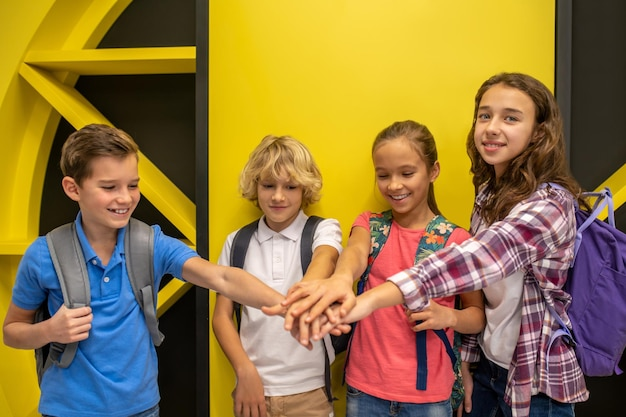
\includegraphics[width=2.18605in,height=1.62945in]{./imgSAEB_6_MAT/media/image21.jpeg}
\end{figure}
\end{quote}

\begin{quote}
\noindent\textbf{Máximo Divisor Comum (M.\,D.\,C.)}

\noindent Exemplo de procedimento de cálculo:

%Tabela 
%A barra indica a divisão entre as duas colunas. MDC entre $20$, $15$ e $10$:
%20, $15$, $10 / 2$ $10$, $15$, $5 / 2$ $5$, $15$, $5 / 5$ $1$, $3$, $1 / 3$ $1$, $1$, $1$

Logo, o M.\,D.\,C. do exemplo acima é $5$, já que é o maior número capaz de
dividir todos os outros.
\end{quote}

\colorsec{Atividades}

\num{1} Adriana e Marina são jogadoras de Vôlei. Em uma partida, Adriana fez
18 pontos e Marina, $17$. Qual é o total de pontos das duas jogadoras?

\reduline{$18 + 17 = 35$.\hfill}

% Professor
% Se achar conveniente, registre as propriedades da adição em um quadro
% que pode ficar afixado em local de fácil visualização para posterior
% consulta dos alunos. 

\noindent Propriedade comutativa: A ordem das parcelas não
altera a soma. Em outras palavras, não importa em que ordem os números
são adicionados, a soma sempre será a mesma. a + b = b + a Exemplo: $7$ +
$4 = 4 + 7$.

\num{2}  Enzo tinha $R\$284,00$ e ganhou de seu pai uma nota de $R\$50,00$. Qual é
o valor total que ele tem agora?

\reduline{$334$ reais.\hfill}

\num{3}  Em um supermercado, há uma balança informando o peso dos alimentos
ali colocados. Aurora pesou suas compras e observou o seguinte resultado
no visor da balança:

\begin{figure}
\centering
\includegraphics[width=2.33333in,height=1.53125in]{./imgSAEB_6_MAT/media/image23.png}
\end{figure}

Após observar o resultado, decidiu pegar mais um item com o peso de
225\,g. Após colocar o item na balança, qual o novo valor observado?

\reduline{$875 + 225 = 1,090\,kg$.\hfill}

\num{4}  A coleção de Celso tem $91$ bolas de gude, e a de Marcelo, $112$. Quantas
bolas de gude os dois possuem juntos?

%Tabela
%https://pixabay.com/pt/photos/m\%c3\%a1rmores-bolinhas-de-vidro-bolas-1659398/. Acesso em $5$ maio $2023$.

\reduline{$203$ Bolinhas de gude.\hfill}

\num{5}  Uma biblioteca municipal contém $3.697$ livros. Considerando que $391$
livros foram emprestados, quantos livros estão nas estantes dessa
biblioteca?

\reduline{$3.306$ livros.\hfill}

\num{6}  No início da semana, uma lanchonete tinha $530$ latas de refrigerante.
Ao longo da semana, foram vendidas $371$ latas. Quantas latas restaram na
lanchonete?

\reduline{$159$ latinhas.\hfill}

\num{7}  Utilizando o método de decomposição em fatores primos, calcule o
M.\,M.\,C. de:

\begin{escolha}
\item $52$ e $78$ \reduline{$156$.\hfill}
\item $8,10,14$ \reduline{$280$.\hfill}
\item $18,42$ \reduline{$126$.\hfill}
\item $12,48$ \reduline{$48$.\hfill}
\item $90,180$ \reduline{$180$.\hfill}
\end{escolha}

\num{8}  Utilizando o método de decomposição em fatores primos, calcule o
M.\,D.\,C. de:

\begin{escolha}
\item $52$ e $78$ \reduline{$78$.\hfill}
\item $8$, $10$, $14$ \reduline{$2$.\hfill}
\item $32$, $48$ \reduline{$16$.\hfill}
\item $60,72$ \reduline{$12$.\hfill}
\end{escolha}

\num{9} Joana comprou $3$ rolos de tecido. O primeiro mede $100\,cm$; o segundo,
$80\,cm$, e o terceiro mede $120\,cm$. Ela pretende dividir os rolos em
pedaços iguais e do maior tamanho possível. Sendo assim, quantos pedaços
terá cada pedaço de tecido?

\begin{escolha}
\item $15\,cm$ \reduline{\hfill}
\item $18\,cm$ \reduline{\hfill}
\item $20\,cm$ \reduline{\hfill}
\item $22\,cm$ \reduline{$100$, $80$, $120 = 20\,cm$.\hfill}
\end{escolha}

\num{10} Laura, Pablo e Josiane trabalham em uma empresa de turismo e viajam
constantemente para o Nordeste. Laura viaja de $10$ em $10$ dias, Pablo de
15 em $15$ dias e Josiane, de $20$ em $20$. Se todos forem hoje para o
nordeste, daqui a quanto tempo eles viajarão no mesmo dia novamente?

\reduline{Daqui a $60$ dias.\hfill}

\num{11} Um tabuleiro de xadrez é todo quadriculado e composto de $8$ linhas e
$8$ colunas. Cada quadradinho é chamado de casa. Quantas casas tem esse
tabuleiro?

% Tabela
% https://pixabay.com/pt/vectors/tabuleiro-de-xadrez-xadrez-conselho-29630/.

\reduline{$64$ casas.\hfill}

\num{12} Calcule as potências abaixo:

\begin{escolha}
\item $5^2$ \reduline{$25$.\hfill}
\item $3^2$ \reduline{$9$.\hfill}
\item $4^3$ \reduline{$64$.\hfill}
\item $7^2$ \reduline{$49$.\hfill}
\item $2^3$ \reduline{$8$.\hfill}
\item $10^3$ \reduline{$1000$.\hfill}
\item $3^3$ \reduline{$27$.\hfill}
\item $8^2$ \reduline{$64$.\hfill}
\end{escolha}

\noindent É interessante explorar a operação potenciação por meio de
situações-problema. Exemplo:

\begin{itemize}
\item Em um estacionamento há $4$ automóveis, em cada automóvel há $4$ rodas e
em cada roda há $4$ parafusos. Qual é o total de parafusos desses $4$
automóveis?

\item Um fazendeiro armazena as laranjas de sua fazenda para vender em
caixas que lembram um cubo. Cada caixa contém $5$ laranjas no comprimento,
5 laranjas na largura e $5$ laranjas na altura. Quantas laranjas podem ser
armazenadas em $5$ caixas?
\end{itemize}

% Professor
% Observar as estratégias dos alunos para resolver as situações propostas.
% É possível que alguns optem em fazer desenhos, esquemas ou optem pelo
% material concreto para auxiliá-los no cálculo.

% Associe essas atividades com a representação de uma
% potenciação. Inicialmente, a linguagem utilizada para definir a
% potenciação e seus elementos pode ser confusa para os alunos. Sempre que
% possível, fazer a identificação desses elementos utilizando exemplos ou
% atividades para que eles possam compreender a nomenclatura correta e as
% ideias ligadas a essa simbologia.

\colorsec{Treino}

\num{1}  Três asteroides se aproximam do sol a cada $20$, $24$, e $28$ anos,
respectivamente. Se o último ano em que todos estiveram próximos do sol
foi $1984$, o próximo ano em que isso deverá ocorrer será?

\begin{escolha}
\item
  $72$
\item
  $840$
\item
  $1988$
\item
  $2824$
\end{escolha}

\paragraph{BNCC: EF06MA06 }
% -- Resolver e elaborar problemas que envolvam as ideias
% de múltiplo e de divisor.
% SAEB: Resolver problemas que envolvam as ideias de múltiplo, divisor,
% máximo divisor comum ou mínimo múltiplo comum.

% Gabarito
% Alternativa A: incorreta, pois o aluno pode realizar a somar a soma ao
% invés de calcular o M.\,M.\,C.
% Alternativa B: incorreta, pois o aluno pode considerar que o valor do
% M.\,M.\,C. em si já é a resposta.
% Alternativa C: incorreta, pois o aluno pode confundir M.\,M.\,C. com M.\,D.\,C.
% nos cálculos e chegar a esse resultado.
% Alternativa D: correta, pois somando o resultado do M.\,M.\,C. com o ano de
% 1984 obtemos este valor.

\num{2}  Entre algumas famílias foram distribuídos $240$ cadernos, $576$ lápis e
$1.080$ borrachas. A distribuição foi feita de tal modo que o maior número
de famílias fosse contemplado e que cada família recebesse o mesmo
número de lápis, o mesmo número de cadernos e o mesmo número de
borrachas. Nessas condições o número de borrachas que cada família
recebeu foi:

\begin{escolha}
\item $24$ 
\item $8$ 
\item $12$ 
\item $45$
\end{escolha}

\paragraph{BNCC: EF06MA07 }
% -- Compreender, comparar e ordenar frações associadas às
% ideias de partes de inteiros e resultado de divisão, identificando
% frações equivalentes.
% SAEB: Resolver problemas que envolvam as ideias de múltiplo, divisor,
% máximo divisor comum ou mínimo múltiplo comum.

% Gabarito
% Alternativa A: incorreta, pois O aluno pode confundir o resultado do
% M.\,D.\,C. dos valores como resposta.
% Alternativa B: incorreta, pois o aluno pode calcular incorretamente o
% M.\,D.\,C. esquecendo do valor $5$ no final, onde o resultado seria esse.
% Alternativa C: incorreta, pois o aluno pode esquecer de contar um número
% ``2'' no cálculo do M.\,D.\,C.
% Alternativa D: correta, pois, calculando o M.\,D.\,C., obtemos $24$,
% realizando a operação $1080$: $24$ obtemos $45$.

\num{3}  Jonas abastece seu veículo a cada $3$ dias e Moises a cada $6$. Paulo vai
abastecer seu veículo sempre aos sábados e em nenhum outro dia. Se no
dia $20$ de setembro os três abasteceram seus veículos, a próxima data em
que os três abastecerão juntos será:

\begin{escolha}
\item $20$ de outubro
\item $2$ de novembro
\item $1$ de novembro
\item $31$ de Outubro
\end{escolha}

\paragraph{BNCC: EF06MA06 }
% -- Resolver e elaborar problemas que envolvam as ideias
% de múltiplo e de divisor.
% SAEB: Resolver problemas que envolvam as ideias de múltiplo, divisor,
% máximo divisor comum ou mínimo múltiplo comum.

% Gabarito
% Alternativa A: incorreta, pois o aluno pode considerar correta essa
% alternativa caso ele considere que se encontram no mesmo dia de todo
% mês.
% Alternativa B: incorreta, pois o aluno pode chegar a esse resultado se
% considerar que outubro tenha $30$ dias.
% Alternativa C: correta, pois realizando o M.\,M.\,C., temos $42$ dias. $20$ dias
% depois de $20$ de setembro cairá no dia $1$ de novembro, lembrando que
% outubro tem $31$ dias.
% Alternativa D: incorreta, pois o aluno pode considerar que setembro
% tenha $31$ dias.

\chapter{Frações}
\markboth{Módulo 3}{}

\colorsec{Habilidades do SAEB}
\begin{itemize}
\item Representar frações menores ou maiores que a
unidade por meio de representações pictóricas ou associar frações a
representações pictóricas.
\item
  Identificar frações equivalentes.
\item
  Determinar uma fração geratriz para uma dízima periódica.
\end{itemize}

\colorsec{Habilidade da BNCC} 
\begin{itemize}
\item EF06MA09.
\end{itemize}

\conteudo{
Uma fração é uma forma de representar uma quantidade ou uma proporção de
um todo que é dividido em partes iguais. Ela é composta por duas partes:
o numerador e o denominador. O numerador representa a quantidade ou a
parte que está sendo considerada, e o denominador representa o total de
partes em que o todo foi dividido.

Por exemplo, a fração $3/4$ representa a parte de um todo que é igual a
três partes em um total de quatro partes iguais. Isso pode ser
visualizado como uma pizza dividida em quatro partes iguais, onde três
dessas partes são consideradas.

As frações podem ser usadas em diversas situações, como na representação
de números decimais em forma de fração, na resolução de problemas que
envolvem proporções ou na medição de quantidades em que um todo é
dividido em partes iguais, como no caso de receitas culinárias.

As frações também podem ser comparadas e operadas matematicamente
através de adição, subtração, multiplicação e divisão, o que permite
realizar cálculos e resolver problemas que envolvem frações.

% Tabela
% https://br.freepik.com/fotos-gratis/graficos-estatisticos-coloridos-para-fracoes-cientificas\_6626366.htm\#query=fractions\&from\_query=fra\%C3\%A7\%C3\%B5es\&position=6\&from\_view=search\&track=sph.
% Acesso em: $5$ maio $2023$.

A comparação entre frações significa olhar para duas frações e descobrir
qual é a maior ou qual é a menor. Para comparar frações, é necessário
deixá-las com o mesmo denominador e ver qual tem o maior numerador.

Por exemplo, a fração $2/3$ é maior que a fração $1/3$, pois o numerador,
isto é, o número de cima é maior. Perceba como o número da parte
inferior da fração, o denominador, é o mesmo.

As~frações equivalentes~são aquelas que, embora aparentemente pareçam
diferentes, possuem o mesmo resultado. Sendo assim, elas representam a
mesma parte de um todo indicando a mesma quantidade.

Por exemplo, a fração $1/2$ é equivalente à fração $2/4$. Para nos
certificarmos desse fato, basta dividirmos o numerador e denominador da
segunda fração por $2$, chegando à fração $1/2$ novamente.

Resgatar com os alunos os conhecimentos que possuem acerca das frações,
para assim aproximar ou relembrar conceitos estudados anteriormente. Se
possível, levar figuras de círculos de cartolina para que os alunos
possam vivenciar as questões propostas nesta seção. Eles podem dividir
as representações dos círculos em pedaços e recortá-los como se fossem
pizzas e realizar diferentes explorações. Vale destacar que é
interessante refletir com os alunos sobre o uso de alimentos para
representar frações, pois muitas vezes uma fatia pode possuir o mesmo
tamanho que outras, mas as massas podem ser diferentes.}

\colorsec{Atividades}

\num{1}  Dois irmãos, Abel e Caim, resolveram comprar uma pizza juntos. Ao
chegar em casa, Abel comeu $3/8$ da pizza, enquanto Caim comeu $7/16$ avos.
Qual dos irmãos comeu a maior parte da pizza?

\reduline{Caim comeu a maior quantidade de pizza pois $3/8$ \textless{} $7/16$.\hfill}

\num{2}  Em um certo dia, Mateus comprou uma barra de chocolate com $24$ pedaços
para dividir igualmente entre seus $3$ filhos. Quantos pedaços cada filho
deve receber?

\reduline{$24$ pedaços para $3$ filhos \textless{} $24$/$3$ = $8$ pedaços cada um.\hfill}\linhas{3}

% Deixar o espaço de $3$ linhas para resolução e Inserir a figura descrita
% acima, podendo ser uma figura semelhante a essa.

\num{3}  Ligue as frações equivalentes:

\begin{mdframed}[linewidth=2pt,linecolor=azul!20,backgroundcolor=azul!20,roundcorner=2pt]
2/4 \hfill 10,5    \rosa{2/4 é ligado a 1/2}
6/7 \hfill 1/5    \rosa{6/7 é ligado a 12/14}
3/4 \hfill 1/2    \rosa{3/4 é ligado a 6/8}
2/1 \hfill 12/14    \rosa{2/1 é ligado a 10/5}
2/10 \hfill 6/8    \rosa{2/10 é ligado a 1/5}
1/3 \hfill 3/9    \rosa{1/3 é ligado a 3/9}
\end{mdframed}

% Tabela
% 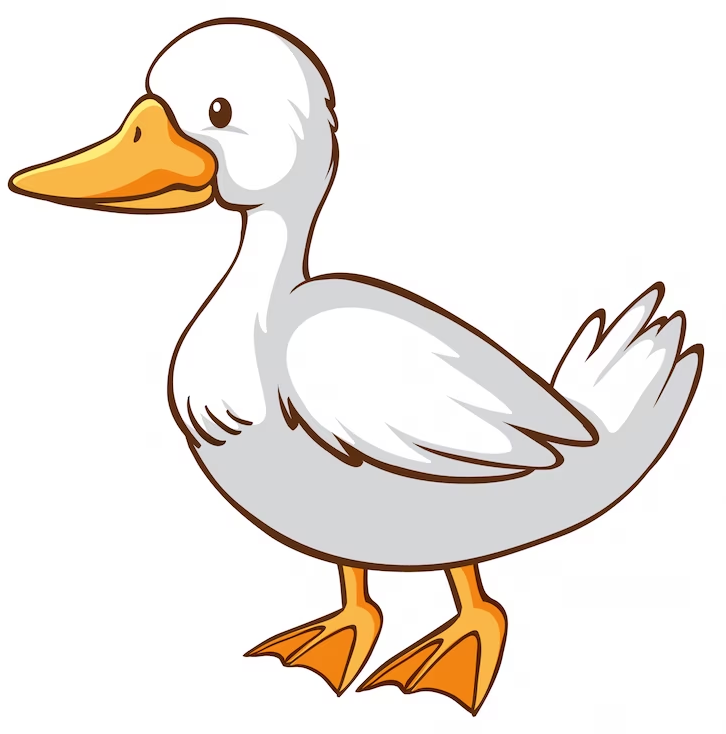
\includegraphics[width=4.35393in,height=2.301in]{./imgSAEB_6_MAT/media/image30.png}
% 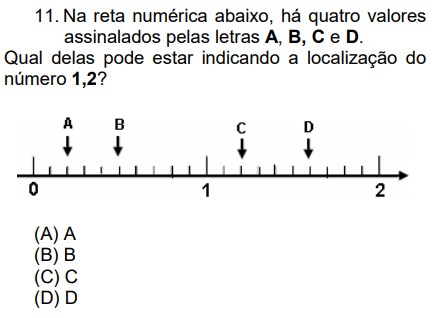
\includegraphics[width=4.5116in,height=2.28926in]{./imgSAEB_6_MAT/media/image31.png}

\num{4}  Para ser aprovado em uma prova, Lucas precisava acertar no mínimo $3/5$
das questões. Ao final do teste, Lucas descobriu que acertou. Sendo
assim, ele foi aprovado ou reprovado?

\reduline{Lucas foi aprovado pois $2/3$ \textgreater{} $3/5$.\hfill}

\num{5}  Sabendo que as figuras foram divididas em partes iguais, em cada
item, escreva a fração correspondente à parte colorida de amarelo.

\begin{figure}

\includegraphics[width=0.7\textwidth]{./imgSAEB_6_MAT/media/image32.png}
\end{figure}

\begin{escolha}
\item \reduline{$7/4$.\hfill}
\item \reduline{$8/5$.\hfill}
\item \reduline{$7/3$.\hfill}
\item \reduline{$14/5$.\hfill}
\item \reduline{$8/12$.\hfill}
\item \reduline{$4/14$.\hfill}
\end{escolha}

\noindent Nestas atividades, reforçar a ideia de fração como parte de um todo.
Quando se trabalha com sua representação geométrica, há necessidade de
fazer a divisão do todo em partes iguais. Quais elementos podem ser representados por meio de uma fração?

\num{6}  Simplifique as frações, tornando-as irredutíveis:

\begin{escolha}
\item $24/60$   \reduline{$2/5$.\hfill}
\item $18/90$   \reduline{$1/5$.\hfill}
\item $27/36$   \reduline{$3/4$.\hfill}
\item $63/81$   \reduline{$7/9$.\hfill}
\item $9/81$   \reduline{$1/9$.\hfill}
\item $7/21$   \reduline{$1/3$.\hfill}
\item $60/80$   \reduline{$3/4$.\hfill}
\end{escolha}

\num{7}  Maria resolveu fazer bolos para vender em sua padaria Em cada
receita, são utilizadas $3/4$ de xícara de farinha de trigo. Em um final
de semana, Maria faz $8$ bolos. Quantas xícaras serão necessárias?

\reduline{$3/4\times 8 = 6$ xícaras.\hfill}

\noindent Grife cada dado do problema de uma cor. Destaque a pergunta, circulando-a, por exemplo,
para identificar o que deve ser respondido. Faça também uma estimativa do resultado antes de elaborar a resposta completa. Pode ser através de desenhos que representem os dados do problema. Por fim, verifique se a resposta está coerente com os dados do problema.

\num{8}  Leonardo resolveu pintar um quadro simples para colocar na parede de
seu quarto. Para pintar o quadro, Leonardo utilizou as cores azul e laranja. Qual
das duas Leonardo usou mais?

\begin{figure}
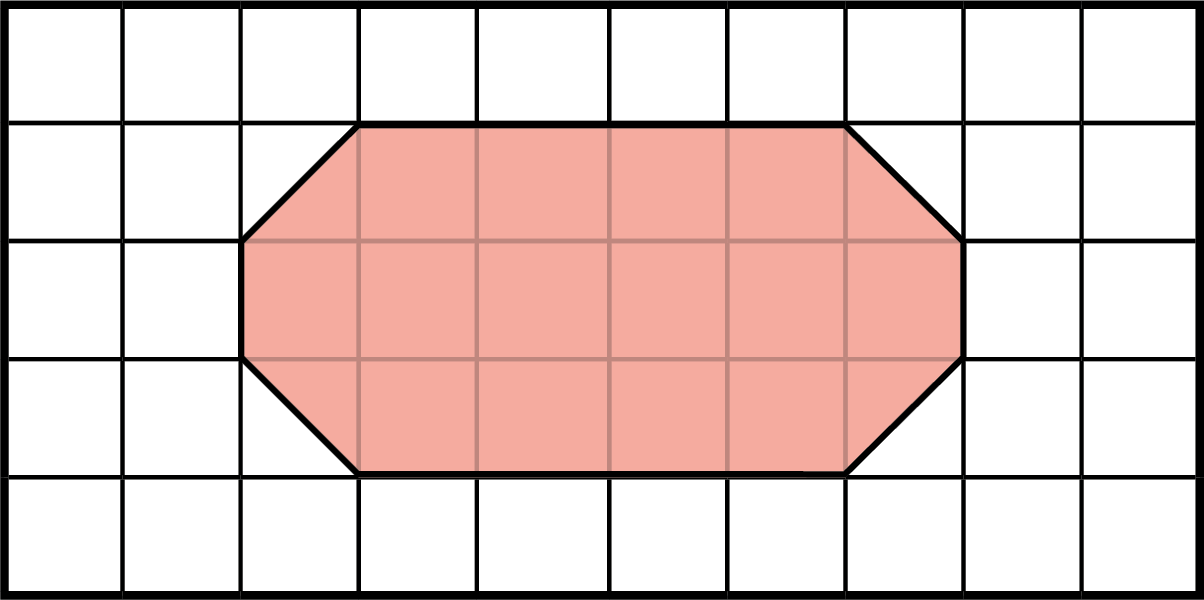
\includegraphics[width=1.58333in,height=1.57292in]{./imgSAEB_6_MAT/media/image33.png}
\end{figure}

\reduline{Leonardo usou no seu quadro $12/16$ avos de tinta azul e $4/16$ avos de
tinta laranja. Como $12/16$ \textgreater{} $4/16$, ele usou mais a tinta
azul.\hfill}

\num{9}  Represente por meio de frações:

\begin{figure}
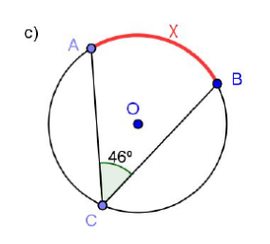
\includegraphics[width=1.61458in,height=4.94792in]{./imgSAEB_6_MAT/media/image34.png}
\end{figure}

\begin{escolha}
\item \reduline{$5/8$.\hfill}
\item \reduline{$6/8$.\hfill}
\item \reduline{$4/6$.\hfill}
\item \reduline{$1/4$.\hfill}
\end{escolha}

% Professor
% Deixar o espaço de $1$ linhas abaixo de cada item para resolução e inserir
% a figura descrita acima, podendo ser uma figura semelhante a essa, porém
% contendo o mesmo conteúdo fracionário.

\num{10} Um prêmio em dinheiro foi dividido entre $4$ amigos em partes
fracionárias. Pedro recebeu $1/6$ do valor, Henrique recebeu $1/2$, Josias
recebeu $1/4$ e Adriano, $1/12$ . Qual dos quatro amigos recebeu a maior
parte do prêmio?

\reduline{Henrique.\hfill}

% Professor
% Com estes exercícios os alunos vão comparar frações por meio da análise
% de seus numeradores e denominadores e desenvolver a ideia de frações
% equivalentes, que será vista a seguir. Destacar que, para comparar as
% frações, é necessário verificar se ambas se referem ao mesmo todo.

\colorsec{Treino}

\num{1}  Em uma padaria, há uma torta que pode ser dividida em $8$ pedaços
iguais. João comeu $3$ desses pedaços, e Maria comeu $2/4$ da torta. Quem
comeu mais torta?

\begin{escolha}
\item João.
\item Maria.
\item João e Maria comeram a mesma quantidade de torta.
\item Não é possível determinar a resposta, pois as frações são diferentes.
\end{escolha}


\paragraph{BNCC: EF06MA09 }
% -- Resolver e elaborar problemas que envolvam o cálculo
% da fração de uma quantidade e cujo resultado seja um número natural, com
% e sem uso de calculadora.
% SAEB: Representar frações menores ou maiores que a unidade por meio de
% representações pictóricas ou associar frações a representações
% pictóricas.

% Gabarito
% Alternativa A: incorreta, pois o aluno provavelmente efetuou a operação
% de maneira incorreta.
% Alternativa B: correta, pois $2/4 = (2 x 2) / (4 x 2) = 4/8$
% $3/8$; logo, Maria comeu mais torta.
% Alternativa C: incorreta, pois a operação demonstra que Maria e João
% comeram porções diferentes.
% Alternativa D: incorreta, pois o aluno deve saber comparar frações
% diferentes.

\num{2}  Um jogo matemático é formado por cartas com frações impressas em uma
de suas faces. Cada jogador recebe quatro cartas e vence aquele que
primeiro conseguir ordená-las crescentemente pelas respectivas frações
impressas. O vencedor foi o aluno que recebeu as cartas com as frações:

$3/5$, $1/4$, $2/3$ e $5/9$. A ordem que esse aluno apresentou foi:

\begin{escolha}
\item $1/4$, $5$/9, $3/5$, $2/3$
\item $1/4$, $2/3$, $3/5$, $5$/9
\item $5$/9, $1/4$, $3/5$, $2/3$
\item $5$/9, $1/4$, $3/5$, $2/3$
\end{escolha}

\paragraph{BNCC: EF06MA09 }
% -- Resolver e elaborar problemas que envolvam o cálculo
% da fração de uma quantidade e cujo resultado seja um número natural, com
% e sem uso de calculadora.
% SAEB: Identificar frações equivalentes.

% Gabarito
% \begin{figure}
% 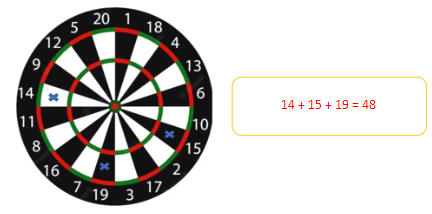
\includegraphics[width=5.01042in,height=1.44792in]{./imgSAEB_6_MAT/media/image36.png}
% \end{figure}

% \noindent Para encontrar as frações equivalentes, dividimos $180$ pelos
% denominadores das frações sorteadas e, multiplicamos o resultado pelos
% numeradores.

% Para $3/5$
% \begin{itemize}
% $180 / 5 = 36$, como $36 x 3 = 108$, a fração equivalente será $108 / 180$.
% \end{itemize}
% Para $1/4$
% \begin{itemize}
% $180/4 = 45$, como $45 x 1 = 45$, a fração equivalente será $45/180$
% \end{itemize}
% Para $2/3$
% \begin{itemize}
% $180/3 = 60$, como $60 x 2 = 120$, a fração equivalente será $120/180$
% \end{itemize}
% Para $5/9$
% \begin{itemize}
% $180/9 = 20$, como $20 x 5 = 100$. A fração equivalente será $100/180$
% \end{itemize}

% Com as frações equivalentes, basta ordenar pelos numeradores em ordem
% crescente e associar com as frações sorteadas. Logo $1/4$, $5$/9, $3/5$, $2/3$.

% Alternativa A: correta, pois: Para comparar frações elas devem possuir os denominadores iguais. Para isso, calculamos o MMC entre $5$, $4$, $3$ e $9$, que são os denominadores das frações sorteadas.
% Alternativa B: incorreta, O aluno pode considerar que quanto maior o
% denominador, maior o valor fracionário, assim $1/4$ seria uma fração maior
% que $2/3$.
% Alternativa C: incorreta, o aluno pode se confundir na forma de calcular
% o M.\,M.\,C. e colocar erroneamente as frações de forma incorreta.
% Alternativa D: incorreta, o aluno pode se confundir e colocar as frações
% em forma decrescente ao invés de crescente.

\num{3}  Elias comprou dois potes de sorvete, ambos com a mesma quantidade do
produto. Um dos potes continha quantidades iguais dos sabores chocolate,
creme e morango; e o outro, quantidades iguais dos sabores chocolate e
baunilha. Então, é CORRETO afirmar que, nessa compra, a fração
correspondente à quantidade de sorvete do sabor chocolate foi:

\begin{escolha}
\item$2/6$ 
\item$3/5$ 
\item$5/12$ 
\item$5/6$
\end{escolha}

\paragraph{BNCC: EF06MA09 }
% -- Resolver e elaborar problemas que envolvam o cálculo
% da fração de uma quantidade e cujo resultado seja um número natural, com
% e sem uso de calculadora.
% SAEB: Representar frações menores ou maiores que a unidade por meio de
% representações pictóricas ou associar frações a representações
% pictóricas

% Gabarito
% Alternativa A: incorreta, pois o aluno pode erroneamente considerar que
% ambos os potes de sorvete foram divididos em $3$ partes.
% Alternativa B: incorreta, pois o aluno erroneamente pode considerar que
% somando as partes de chocolates de ambos os potes sem calcular o M.\,M.\,C.
% pode se tornar uma resposta correta.
% Alternativa C: correta, pois: o primeiro pote continha $3$ sabores em
% iguais quantidades: $1/3$ de chocolate, $1/3$ de baunilha e $1/3$ de morango.
% No segundo pote, havia $1/2$ de chocolate e $1/2$ de baunilha. Considerando
% os dois potes de sorvete, dividimos os dois potes em partes iguais.
% Fazendo então o M.\,M.\,C. de (2,3), obtemos que cada pote foi dividido em $6$
% partes iguais. Portanto nos dois potes temos $12$ partes iguais. Sendo que
% destas, $5$ partes correspondem ao sabor chocolate.
% Alternativa D: incorreta, o aluno pode considerar dividir os potes em $3$
% partes iguais e somar sem calcular o M.\,M.\,C., que chegará a esse
% resultado erroneamente.

\chapter{Porcentagem}
\markboth{Módulo 4}{}

\colorsec{Habilidade do SAEB} 
\begin{itemize}
\item Resolver problemas que envolvam porcentagens,
incluindo os que lidam com acréscimos e decréscimos simples, aplicação
de percentuais sucessivos e determinação de taxas percentuais.
\end{itemize}

\colorsec{Habilidade da BNCC} 
\begin{itemize}
\item EF06MA13
\end{itemize}

\conteudo{
\textbf{Definição}\\

\noindent Porcentagem é uma forma de expressar uma proporção ou uma parte de um
todo em termos de uma base de $100$ unidades. O símbolo ``\%'' é usado
para indicar porcentagem. Por exemplo, se uma empresa tem $100$
funcionários e $50$ deles são mulheres, podemos dizer que $50\%$ dos
funcionários são mulheres. A porcentagem é amplamente utilizada em
finanças, negócios, estatísticas, ciência, entre outras áreas, para
expressar a parte de um todo ou uma taxa de crescimento ou decréscimo em
relação a uma base de $100$.

\textbf{Acréscimo}\\

\noindent Acréscimo é o aumento no valor de um produto ou serviço, que pode ser
expresso em valores absolutos ou em porcentagem. O acréscimo pode
ocorrer por diversos motivos, como a adição de novas funcionalidades ou
recursos a um produto, a valorização de um bem ou serviço ou a variação
dos custos de produção.

Por exemplo, se o preço de um produto é $R\$100,00$ e houve um acréscimo
de $10\%$, o novo preço será $R\$110,00$. O cálculo do preço com acréscimo é
feito multiplicando o preço original pela porcentagem de acréscimo (em
forma decimal), e adicionando o resultado ao preço original:

Preço com acréscimo = Preço original + (Preço original x Porcentagem de
acréscimo)

\textbf{Desconto}\\

\noindent Desconto é uma redução no preço de um produto ou serviço, geralmente
oferecida como uma forma de incentivar as vendas ou recompensar os
clientes. O desconto é expresso em porcentagem e é aplicado ao preço
original do produto ou serviço.

Por exemplo, se um produto tem um preço original de $R\$100,00$ e há um
desconto de $20\%$, o preço com desconto será $R\$80,00$. O cálculo do preço
com desconto é feito multiplicando o preço original pela porcentagem de
desconto (em forma decimal), e subtraindo o resultado do preço original:

Preço com desconto = Preço original \textless{} ($Preço original$ \times $Porcentagem de desconto$)}

\colorsec{Atividades}

\num{1}  Calcule as porcentagens abaixo

\begin{escolha}
\item $1\%$ de $120$ \reduline{$1,2$.\hfill}
\item $50\%$ de $260$ \reduline{$130$.\hfill}
\item $10\%$ de $1300$ \reduline{$130$.\hfill}
\item $25\%$ de $9$ \reduline{$2,25$.\hfill}
\item $30\%$ de $120$ \reduline{$36$.\hfill}
\item $5\%$ de $90$ \reduline{$4,5$.\hfill}
\item $2\%$ de $310$ \reduline{$6,2$.\hfill}
\item $45\%$ de $195$ \reduline{$87,75$.\hfill}
\item $33\%$ de $125$ \reduline{$41,25$.\hfill}
\item $90\%$ de $1700$ \reduline{$1530$.\hfill}
\item $70\%$ de $1745$ \reduline{$1221,5$.\hfill}
\item $0,5\%$ de $205$ \reduline{$1,025$.\hfill}
\item $2,5\%$ de $25$ \reduline{$0,625$.\hfill}
\end{escolha}

\noindent Existem muitos materiais manipuláveis que podem contribuir para o
ensino-aprendizagem deste conteúdo. Um deles é o material dourado, que
pode ser explorado para facilitar o entendimento da relação entre as
frações e as porcentagens. Monte um quadrado com 10 unidades de lado utilizando os cubinhos. Depois divida o quadrado em dois retângulos iguais. 

\begin{itemize}
\item Que fração representa cada retângulo comparado com o quadrado inicial?
\item Cada retângulo representa quantos por cento do quadrado inicial?
\end{itemize}

% Professor
% Provavelmente, os alunos responderão que representa a metade do todo, ou
% seja, $50\%$. Espera-se que os alunos percebam que, para determinar $50\%$
% de um valor, basta dividir esse valor por dois. É interessante fazer
% perguntas como essas para que os alunos percebam que, para determinar
% 25\% de um valor qualquer, basta dividir esse valor por $4$; para
% determinar $20\%$, divide-se por $5$ e, para determinar $10\%$, divide-se por
% 10

\num{2}  Marly tem um salário atual de $R\$1.250,00$. Seu novo patrão irá
aumentar seu salário em $15\%$. Qual o valor do novo salário dela?

\reduline{$R\$1.437,50$.\hfill}

\num{3}  Uma televisão em uma loja de departamentos custa $R\$3.800,00$. Como José adquiriu uma TV e efetuou pagamento à vista, recebeu um
desconto no valor de $15\%$ no produto. Nestas condições, qual foi a
quantia paga por José?

\reduline{$R\$3.230,00$.\hfill}

\num{4}  Uma universidade resolveu iniciar uma pesquisa para saber o perfil
dos seus alunos. Foi descoberto que $46\%$ dos alunos são homens. Sabendo
que a faculdade possui $1.250$ alunos, quantas mulheres estudam nessa
universidade?

\reduline{$675$ Mulheres estudam na universidade.\hfill}

\num{5}  O campeonato brasileiro de futebol possui $38$ rodadas. Para cada
vitória, a equipe ganha $3$ pontos. Sendo assim, a pontuação máxima a ser
alcançada é de $114$ pontos. Sabendo que a equipe vencedora do ano de $2022$
obteve $81$ pontos, qual a porcentagem de pontos alcançada?

\reduline{A equipe campeã alcançou $71,05\%$ dos pontos disputados.\hfill}

\num{6}  Em janeiro, um brinquedo custava $R\$90,00$. Devido à queda nas
vendas, seu preço sofreu uma redução de $20\%$, mantendo-se este valor até
novembro. Com o aquecimento das vendas de Natal, houve um aumento de
10\%. O brinquedo passou a ser vendido por:

\reduline{O brinquedo passou a ser vendido por $R\$79,20$.\hfill}

\num{7}  Uma pesquisa constatou que, no ano de $2021$, uma cidade do interior de
São Paulo possuía $25.000$ habitantes. Considerando que no ano de $2022$
houve um aumento de $6\,\%$ na população, quantos habitantes havia nessa
cidade no ano de $2022$?

\reduline{Em $2022$, a população dessa cidade era de $26.500$ habitantes.\hfill}

\num{8}  Elias foi ao supermercado e constatou que o pacote de arroz de $5$kg
custava $R\$21,50$. No mês seguinte, o mesmo produto custava $R\$23,10$.
Qual foi o acréscimo em \% do arroz?

\reduline{O arroz teve um acréscimo de $6,92\%$.\hfill}

\num{9}  Em uma loja, o preço de um determinado par de calçados era
$R\$120,00$. Durante uma liquidação, ele era vendido por $R\$81,00$. Em
relação ao preço original, o desconto dado corresponde a uma taxa de:

\reduline{O desconto dado foi de $32,5\%$.\hfill}

\num{10}  Uma loja oferece $10\%$ de desconto na compra de $1$ produto, $20\%$ na
compra de $2$ produtos e $30\%$ na compra de $3$ produtos. Adriano quer
comprar camisas com o preço unitário de $R\$80,00$. Quanto Adriano
pagaria\ldots{}

\begin{escolha}
\item na compra de apenas $1$ camisa? \reduline{$R\$72,00$.\hfill}
\item na compra de $2$ camisas? \reduline{$R\$64,00$.\hfill}
\item na compra de $3$ camisas? \reduline{$R\$56,00$.\hfill}
\end{escolha}

\num{11}  Uma pessoa comprou um terreno por $R\$20.000,00$ e o vendeu com o
lucro de $R\$4.000,00$. Qual a porcentagem de lucro?

\reduline{$20\%$ de lucro.\hfill}

\colorsec{Treino}

\num{1}  Em uma determinada cidade, as passagens de ônibus custavam $R\$1,20$. O
novo prefeito reajustou esse valor em $25\%$. Qual será o novo valor das
passagens?

\begin{escolha}
\item $R\$1,45$.
\item $R\$1,23$.
\item $R\$1,25$.
\item $R\$1,50$.
\end{escolha}

\paragraph{BNCC: EF06MA13 }
% -- Resolver e elaborar problemas que envolvam
% porcentagens, com base na ideia de proporcionalidade, sem fazer uso da
% ``regra de três'', utilizando estratégias pessoais, cálculo mental e
% calculadora, em contextos de educação financeira, entre outros.
% SAEB: Resolver problemas que envolvam porcentagens, incluindo os que
% lidam com acréscimos e decréscimos simples, aplicação de percentuais
% sucessivos e determinação de taxas percentuais.

% Gabarito
% Alternativa A: incorreta, pois o aluno pode considerar que aumentar $25\%$
% signifique aumentar $25$ centavos.
% Alternativa B: incorreta, pois o aluno pode calcular erroneamente $1,20$ x
% 0,025, chegando a esse resultado equivocado.
% Alternativa C: incorreta, poiso aluno pode considerar que $25\%$ tenha
% relação com o valor $R\$1,25$, pela semelhança.
% Alternativa D: correta, pois $R\$1,20 x 0,25 = 0,3$, logo somando $R\$1,20$
% + $R\$0,30$ temos $1,50$

\num{2}  Uma livraria realizará uma liquidação e, para isso, o gerente pediu
para Ariane multiplicar todos os preços dos livros por $0,68$. Nessa
liquidação, a loja está oferecendo um desconto de:

\begin{escolha}
\item $68\%$
\item $6,8\%$
\item $3,2\%$
\item $32\%$
\end{escolha}

\paragraph{BNCC: EF06MA13 }
% -- Resolver e elaborar problemas que envolvam
% porcentagens, com base na ideia de proporcionalidade, sem fazer uso da
% ``regra de três'', utilizando estratégias pessoais, cálculo mental e
% calculadora, em contextos de educação financeira, entre outros.
% SAEB: Resolver problemas que envolvam porcentagens, incluindo os que
% lidam com acréscimos e decréscimos simples, aplicação de percentuais
% sucessivos e determinação de taxas percentuais.

% Alternativa A: incorreta, pois aluno pode deduzir que ao multiplicar o
% valor por $0,68$ que o valor logo terá $68\,\%$ de desconto.
% Alternativa B: incorreta, pois o aluno pode deduzir que, ao multiplicar
% o valor por $0,68$, os livros terão $6,8\,\%$ devido à semelhança dos termos.
% Alternativa C: incorreta, pois o cálculo pode ser feito corretamente mas
% a semelhança de $3,2\%$ para $32\%$ pode confundir o aluno na hora de
% decisão de assinalar a resposta correta.
% Alternativa D: correta, pois, ao multiplicar qualquer valor de livro por
% 68\%, obtém-se um desconto de $32\%$.

\num{3}  Em uma loja, uma máquina de lavar roupas custava $R\$1.500,00$ e seu
preço sofreu um aumento de $3\%$. Logo após o aumento, a loja resolveu
fazer uma promoção oferecendo um desconto de $3\%$ no mesmo produto. Qual
o valor do produto após o aumento? E após o desconto, ou seja, após as
duas operações?

\begin{escolha}
\item $R\$1.555,00$ com aumento e $R\$1.498,65$ com desconto.
\item $R\$1.545,00$ com aumento e $R\$1.500,00$ com desconto.
\item $R\$1.545,00$ com aumento e $R\$1.498,65$ com desconto.
\item $R\$1.555,00$ com aumento e $R\$1.500,00$ com desconto.
\end{escolha}

\paragraph{BNCC: EF06MA13 }
% -- Resolver e elaborar problemas que envolvam
% porcentagens, com base na ideia de proporcionalidade, sem fazer uso da
% ``regra de três'', utilizando estratégias pessoais, cálculo mental e
% calculadora, em contextos de educação financeira, entre outros.
% SAEB: Resolver problemas que envolvam porcentagens, incluindo os que
% lidam com acréscimos e decréscimos simples, aplicação de percentuais
% sucessivos e determinação de taxas percentuais.

% Gabarito:
% Alternativa A: incorreta, pois o aluno pode realizar o cálculo
% corretamente, mas confundir os valores próximos de R\$1.555, $00$ com
% R\$1.545, $00$ devido à semelhança.
% Alternativa B: incorreta, pois o aluno, por meio de dedução, pode
% considerar que, somando $3\%$ ao valor inicial e subtraindo $3\%$, o valor
% inicial fique inerte.
% Alternativa C: Correta. Cálculo do acréscimo: $1500\times 0,03 = 45$; $1.550 + 45 = 1.545$. Cálculo do desconto: $1.545\times 0,03 = 46,35$; $1.545 - 46,35 = 1.498,65$.
% Alternativa D: incorreta, pois o aluno, por meio de dedução, pode
% considerar que, somando $3\%$ ao valor inicial e subtraindo $3\%$, o valor
% inicial fique inerte.

\chapter{Equações polinomiais}
\markboth{Módulo 5}{}

\colorsec{Habilidades do SAEB} 
\begin{itemize}
\item Resolver uma equação polinomial de 1º grau.
\item
 Resolver uma equação polinomial de 1º grau.
\item
  Inferir uma equação, inequação polinomial de 1º grau ou um sistema de
  equações de 1º grau com duas incógnitas que modela um problema.
\item
  Associar uma equação polinomial de 1º grau com duas variáveis a uma
  reta no plano cartesiano.
\item
  Resolver problemas que possam ser representados por sistema de
  equações de 1º grau com duas incógnitas.
\end{itemize}

\colorsec{Habilidades da BNCC}
\begin{itemize} 
\item  EF06MA14
\end{itemize}

\conteudo{
\noindent A equação do 1º grau é uma equação que possui uma incógnita com grau 1, ou seja, a incógnita está elevada a potência 1.

$a\times x + b = 0$, em que a e b são números reais, e a é diferente de $0$.

Sistema com equações de 1º grau. Exemplo: $$x + y = 20 3x + 4y = 72$$.

Método da substituição Esse método consiste em escolher uma das duas
equações, isolar uma das incógnitas e substituir na outra equação, veja
como:

Dado o sistema,

$$x + y = 40$$
$$3x + 4y = 144$$

Enumeramos as equações.

\num{1}  $x + y = 40$
\num{2}  $3x + 4y = 144$

Escolhemos a primeira equação e isolamos o $X$:

$$x + y = 40 x = 40 - y$$

Agora, na equação $2$, substituímos o valor de $x = 40 - y$.

$$3x + 4y = 144$$ 
$$3 (40 - y) + 4y = 144 120 - 3y + 4y = 144 y = 24$$

Descobrimos o valor de $Y$. Para descobrir o valor de $X$, basta substituir
o $Y$ na equação:

$$x = 40 - y x = 40 - 24 x = 16$$

Portanto, a solução do sistema é $S = (16, 24)$.
}

\colorsec{Atividades}

\num{1}  Resolva as Equações polinomiais abaixo e descubra o valor de X em
cada uma delas:

\begin{itemize}
\item $x + 5 = 8$ \reduline{$3$.\hfill}
\item $x − 4 = 3$ \reduline{$7$.\hfill}
\item $x + 9 = −1$ \reduline{$-10$.\hfill}
\item $4x − 9 = 23$ \reduline{$8$.\hfill}
\item $7x − 33 = −12$ \reduline{$3$.\hfill}
\item $33+ x = 5 -- 3x$ \reduline{$-7$.\hfill}
\item $3(x + 2) = 2 (x - 7)$ \reduline{$-20$.\hfill}
\item $2x - 10 + 7x + 10 = 180$ \reduline{$20$.\hfill}
\end{itemize}

\num{2}  Responda às sentenças abaixo.

\begin{enumerate}\def\labelenumi{\alph{enumi})}
\item O dobro de um número somado com $5$ é igual a $91$. Qual é esse número? \reduline{$x = 43$.\hfill}
\item O triplo de um número diminuído de $4$ é igual a $23$. Qual é esse número? \reduline{$x = 9$.\hfill}
\item O número somado com o seu dobro é igual a $150$. Qual é esse número? \reduline{$x = 50$.\hfill}
\item Qual é o número que, adicionado a $28$, é igual a $3$ vezes esse número? \reduline{$x = 14$.\hfill}
\item O triplo de um número menos $10$ é igual ao próprio número mais $70$. Qual é esse número? \reduline{$x = 40$.\hfill}
\item Noêmia é $5$ anos mais velha que Ágata. A soma das idades dá $43$ anos. Qual a idade de Ágata? \reduline{Ágata tem $19$ anos..\hfill}
\item Quando Manoel nasceu, Carlos tinha $3$ anos. Atualmente, a soma das idades é $23$ anos. Qual é a idade de Carlos? \reduline{Carlos tem $13$ anos..\hfill}
\end{enumerate}

\num{3}  Os $1.200$ alunos matriculados numa escola estão assim distribuídos: no
período da manhã, há $320$ alunos a mais do que no período da tarde e, à
noite, há $190$ alunos a menos do que no período da manhã. O número de
alunos do período da manhã desta escola é?

\reduline{$570$.\hfill}

\num{4}  Resolva os sistemas formados pelas equações abaixo.

\begin{escolha}
\item $x + y = 1$; $4x + 7y = 10$ \reduline{Solução: $x = -1, y = 2$.\hfill}
\item $3x + y = 13$; $x - 2y = 2$ \reduline{Solução: $x = 4, y = 2$.\hfill}
\item $2x + y = 5$; $x - y = 1$ \reduline{Solução: $x = 1, y = 2$.\hfill}
\item $x + y = 4$; $3x + 2y = 9$ \reduline{Solução: $x = 2, y = 1$.\hfill}
\item $x + y = 10$; $2x - y = 8$ \reduline{Solução: $x = 1, y = 3$.\hfill}
\end{escolha}

% Professor
% Verificar % Tem um exercício a mais! Entender resposta correta.
%\reduline{Solução: $x = 6, y = 4$.\hfill}

\num{5}  Em um determinado mês, duas montadoras produziram, juntas, $77.500$
veículos, sendo que a produção de x foi igual a $2/3$ da produção de y. Nesse mês, a quantidade de veículos produzidos por x foi:

\reduline{$46.500$.\hfill}

\num{6}  Numa cantina, $2$ copos de suco e $3$ pastéis custam $R\$5,70$. O preço de
3 copos de suco e $5$ pastéis é $R\$9,30$. Quanto custa cada pastel e cada
copo de suco?

\reduline{Cada pastel custa $R\$1,50$ e cada suco custa $R\$0,60$.\hfill}

\num{7}  Considerando a equação $5(3x - 8) = -45$, é correto afirmar que a equação equivalente a ela é:

\reduline{$15x + 5 = 0$.\hfill}

\num{8}  Uma região retangular foi totalmente cercada por uma tela. A figura a
seguir mostra as medidas dos lados, em metros, dessa região.

\begin{figure}
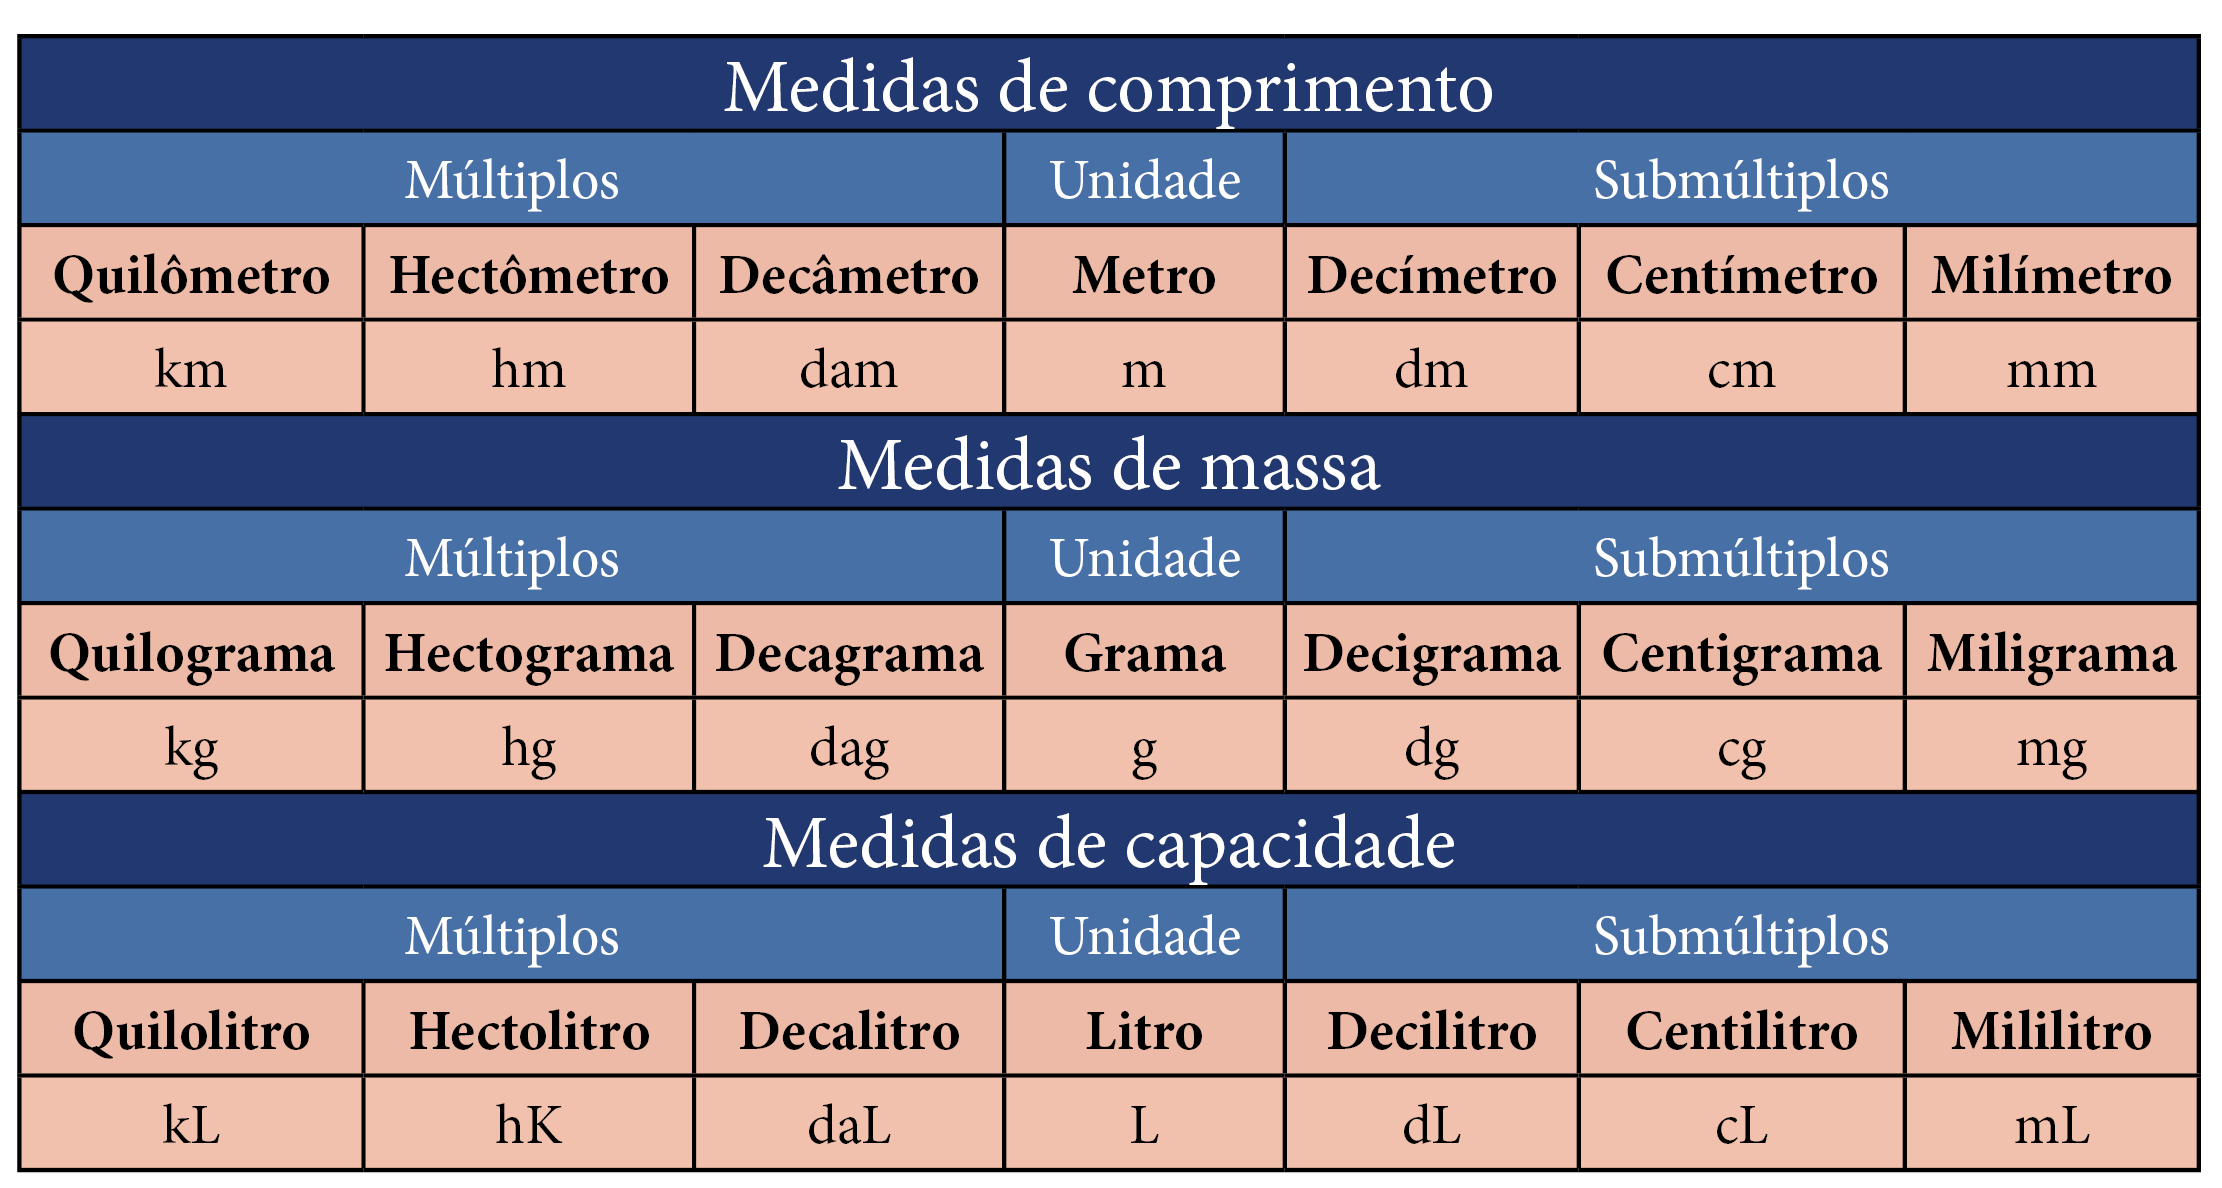
\includegraphics[width=1.65625in,height=1.14583in]{./imgSAEB_6_MAT/media/image38.png}
\end{figure}

Se para cercar totalmente essa região foram utilizados $24$ m de tela, a
medida do lado menor é igual a:

\reduline{$4$.\hfill}

\num{9} Numa loja, algumas camisetas e calças estão em oferta. $3$ calças e $2$
camisetas são vendidas por $R\$56,00$. Por sua vez, $2$ calças e $1$ camiseta
saem por $R\$34,00$. O preço unitário da calça e da camiseta pode ser
determinado a partir da solução do sistema:

\reduline{$3x + 2y = 56$\\
$2x + y = 34$.\hfill}

\colorsec{Treino}

\num{1}  Numa caixa, há bolas Vermelhas e bolas amarelas num total de $360$
esferas. Se o número de bolas vermelhas é o quádruplo do de amarelas, o
número de bolas vermelhas é:

\begin{escolha}
\item $18$
\item $72$
\item $90$
\item $288$
\end{escolha}

\paragraph{BNCC: EF06MA14 }
% -- Reconhecer que a relação de igualdade matemática não
% se altera ao adicionar, subtrair, multiplicar ou dividir os seus dois
% membros por um mesmo número e utilizar essa noção para determinar
% valores desconhecidos na resolução de problemas.
% SAEB: Resolver problemas que possam ser representados por sistema de
% equações de 1º grau com duas incógnitas.

% Gabarito
% Alternativa A: incorreta, pois o aluno pode chegar à conclusão de que o
% número de bolas vermelhas é $72$, dividindo por $4$ ao tentar encontrar o
% número de bolas amarelas.
% Alternativa B: incorreta, pois o aluno pode considerar que o enunciado
% pede o número de bolas amarelas.
% Alternativa C: incorreta, pois o aluno pode realizar a operação $360$:4,
% obtendo um resultado incorreto.
% Alternativa D: correta, pois, realizando o sistema, temos que: $X + Y = 360$; $X = 4y$. Inserindo o valor de X na primeira equação, temos que: $4y + y = 360$; $5y = 360$; $y = 72$. Realizando $360 - 72 = 288$, temos o valor correto de bolas vermelhas.

\num{2}  O tempo t, em segundos, que uma pedra leva para cair de uma altura x,
em metros, é dado aproximadamente pela fórmula $t = 0,05$x. Se o tempo t
da queda é de $8$ segundos, a altura x é:

\begin{escolha}
\item $0,4$ m
\item $0,00625$ m
\item $160$ m
\item $4$ m
\end{escolha}

\paragraph{BNCC: EF06MA14 }
% -- Reconhecer que a relação de igualdade matemática não
% se altera ao adicionar, subtrair, multiplicar ou dividir os seus dois
% membros por um mesmo número e utilizar essa noção para determinar
% valores desconhecidos na resolução de problemas.
% SAEB: Resolver problemas que possam ser representados por sistema de
% equações de 1º grau com duas incógnitas.

% Gabarito
% Alternativa A: incorreta, pois o aluno durante a resolução pode
% confundir e ao invés de dividir $8$ por $0,05$, realizar a multiplicação.
% Alternativa B: incorreta, pois o aluno pode resolver a equação
% erroneamente, calculando $0,05$ : $8$.
% Alternativa C: correta, pois, ao substituir t por $8$, temos: $$8 = 0,05 . x$$; $$8/0,05 = x$$; $$x = 160$$.
% Alternativa D: incorreta, pois o aluno pode erroneamente colocar o valor
% 8 na incógnita x.

\num{3}  Dois produtos químicos A e B são usados em um laboratório. Cada $1$ g
(grama) do produto A custa $R\$0,03$, e cada $1$ g do produto B custa R\$
0,05. Se $100\,g$ de uma mistura dos dois produtos custam $R\$3,60$, a
quantidade do produto A contida nesta mistura é:

\begin{escolha}
\item $70\,g$
\item $100\,g$
\item $360\,g$
\item $140\,g$
\end{escolha}

\paragraph{BNCC: EF06MA14 }
% -- Reconhecer que a relação de igualdade matemática não
% se altera ao adicionar, subtrair, multiplicar ou dividir os seus dois
% membros por um mesmo número e utilizar essa noção para determinar
% valores desconhecidos na resolução de problemas.
% SAEB: Resolver problemas que possam ser representados por sistema de
% equações de 1º grau com duas incógnitas.

% Gabarito
% Alternativa A: Correta. Considerando que x = quantidade do produto A em gramas; y = quantidade do produto B em gramas. $x + y = 100$ (I); $x·A + y·B = 3,60$ (II). De (I), deduzimos: $y = 100 - x$. Que aplicamos em (II): $x·A + (100-x)·B = 3,60$. Substituindo A e B pelos seus custos em reais: $x·0,03 + (100-x)y·0,05 = 3,60$. Multiplicando toda a equação acima por $100$, a fim de tornar inteiros
% seus coeficientes: $x·3 + (100-x)·5 = 360$; $3x + 500 - 5x = 360$; $-2x = 360 - 500$; $-2x = -140$; $x = -140/-2$; $x = 70$ gramas. 
% Alternativa B: incorreta, pois o aluno pode simplesmente retirar a
% quantidade de gramas do enunciado e considerar como resposta correta.
% Alternativa C: incorreta, pois o aluno pode considerar o preço final do
% produto como resposta correta.
% Alternativa D: incorreta, pois o aluno pode esquecer de dividir a
% equação final por $2$, chegando a esse resultado.

\chapter{Proporções}
\markboth{Módulo 6}{}

\colorsec{Habilidade do SAEB} 
\begin{itemize}
\item Resolver problemas que envolvam variação de
proporcionalidade direta ou inversa entre duas ou mais grandezas,
inclusive escalas, divisões proporcionais e taxa de variação.
\end{itemize}

\conteudo{
Neste módulo, falaremos sobre variações direta e inversamente
proporcionais. Comecemos discutindo alguns tipos de razões:

\noindent\textbf{Escala}\\
\noindent A razão de escala é uma relação matemática que indica a proporção
entre as dimensões de duas figuras semelhantes. Ela é dada pela razão
entre as medidas de um mesmo lado (ou altura, ou diagonal, etc.) das
duas figuras.

Por exemplo, se duas figuras são semelhantes e o lado da primeira figura
mede $5\,cm$ e o lado correspondente da segunda figura mede $10\,cm$, a razão
de escala entre as duas figuras é $10/5$ ou $2/1$.

\noindent\textbf{Velocidade Média}\\
Velocidade média é uma grandeza física que representa a
variação de espaço (distância percorrida) em relação ao tempo gasto para
percorrê-lo. Ela é dada pela razão entre a distância percorrida e o
tempo gasto: \textit{$Velocidade média = Distância percorrida / Tempo gasto$}

\noindent\textbf{Densidade}\\
Densidade é uma grandeza física que representa a quantidade de
massa presente em um determinado volume. Ela é calculada pela razão
entre a massa de um objeto e o volume ocupado por ele. A fórmula da densidade é: \textit{$Densidade = \frac{Massa}{Volume}$}

\noindent\textbf{Densidade demográfica}\\

\noindent A densidade demográfica é uma medida que indica a
relação entre a população de uma determinada área e a sua superfície.
Ela é obtida dividindo-se o número de habitantes pela área total da
região.

Por exemplo, se uma cidade tem uma população de $100.000$ habitantes e sua
área total é de $50$ km², sua densidade demográfica é de $2.000$ habitantes
por km².

Todos esses tipos de razão podem seguir uma lógica direta ou
inversamente proporcional.}

\begin{quote}
\begin{itemize}
\item Grandezas \textit{diretamente} proporcionais\quad Duas grandezas são diretamente proporcionais quando ambas aumentam ou
ambas diminuem na mesma proporção.
\item Grandezas \textit{inversamente} proporcionais\quad Duas grandezas são inversamente proporcionais quando uma aumenta e outra
diminui na mesma proporção.
\end{itemize}
\end{quote}

\colorsec{Atividades}

\num{1}  Para se construir uma calçada, é comum, na constituição do concreto,
se utilizar cimento, areia e brita na seguinte proporção: $1$ parte de
cimento, $4$ partes de areia e $2$ partes de brita. Para construir o
calçada, uma construtora encomendou um caminhão betoneira com $14$ m³ de
concreto. Qual é o volume de cimento, em m³, na carga de concreto
trazido pela betoneira?

\reduline{$2$ m³\hfill}

\num{2}  Josué tem ração suficiente para alimentar quatro animais durante $18$
dias. No fim do $6$º dia, ele comprou mais dois animais. Com o restante da
ração, ele poderá alimentar seus animais durante:

\reduline{$8$ dias.\hfill}

\num{3}  Num teste, uma pessoa acertou $12$ de $20$ questões. A razão do número de
questões erradas para o número total de questões é:

\reduline{$2/5$\hfill}

\num{4}  Uma rua tem $800$ m de comprimento e está sendo asfaltada. Em seis
dias, foram asfaltados $200$ m da rua. Supondo-se que o ritmo de trabalho
continue o mesmo, qual o total de dias empreendidos no asfaltamento?

\reduline{$24$ dias.\hfill}

\num{5}  Dez operários constroem uma parede em $10$ horas. Quantos operários
serão necessários para construir a mesma parede em $2$ horas?

\reduline{$50$ operários.\hfill}

\num{6}  Sílvia fará um bolo para a festa da primavera. Para cada pacote de
mistura para bolos, Sílvia deve usar $2$ ovos. Quantos pacotes dessa
mistura serão necessários se ela usar $10$ ovos?

\reduline{$5$ pacotes.\hfill}

\num{7}  Para fazer um determinado serviço, $5$ engenheiros levam $40$ dias. Em
quanto tempo $10$ engenheiros fazem o mesmo serviço?

\reduline{$80$ dias.\hfill}

\num{8}  Para atender todas as ligações telefônicas que recebe, uma empresa
emprega $4$ telefonistas que atendem, cada uma, $120$ ligações por dia. Se a
empresa utilizasse $6$ telefonistas, cada uma atenderia,

\reduline{$120$ ligações.\hfill}

\num{9}  Uma torneira despeja $16$ litros por minuto e enche uma caixa em $5$
horas. Quanto tempo levará para encher a mesma caixa uma torneira que
despeja $20$ litros por minuto?

\reduline{$5$ horas.\hfill}

\num{10}  Podemos transportar uma determinada quantidade de pedras em $20$
caminhões com capacidade de $7$ m³ cada. Caso utilize caminhões com
capacidade para $14$ m³, precisaríamos de:

\reduline{$10$ caminhões.\hfill}

\colorsec{Treino}

\num{1}  Em uma indústria, $20$ máquinas iguais, de mesmo rendimento, produzem
juntas $5.000$ peças iguais, em meia hora de funcionamento simultâneo e
ininterrupto. Desse modo, para produzir $1.000$ unidades das mesmas peças
em uma hora, seria necessário o funcionamento, nas mesmas condições
operacionais, de apenas:

\begin{escolha}
\item $2$ máquinas.
\item $4$ máquinas.
\item $100$ máquinas.
\item $200$ máquinas.
\end{escolha}

% SAEB: Resolver problemas que envolvam variação de proporcionalidade
% direta ou inversa entre duas ou mais grandezas, inclusive escalas,
% divisões proporcionais e taxa de variação.

% Gabarito
% Alternativa A: correta, pois, ao realizar a regra de $3$ simples, obtemos
% o valor de $2$ máquinas.
% Alternativa B: incorreta, pois o aluno pode esquecer de realizar a
% conversão de uma hora para meia hora, chegando a esse resultado
% erroneamente.
% Alternativa C: incorreta, pois o aluno pode, ao invés de realizar o
% cruzamento na regra de três, multiplicar linearmente, chegando a esse
% resultado.
% Alternativa D: O aluno pode realizar a conversão corretamente, mas errar
% o cruzamento no cálculo de regra de três, chegando a esse valor
% erroneamente.

\num{2}  Para imprimir $200$ apostilas com $27$ páginas cada, $5$ impressoras levam
54 minutos. Estas impressoras imprimem um mesmo número de páginas por
minuto e têm um sistema automático de alimentação de folhas, ou seja,
não precisam parar para o reabastecimento. Para a impressão de $1.040$
apostilas com $35$ páginas impressas cada uma em $52$ minutos, seriam
necessárias

\begin{escolha}
\item $2$ impressoras.
\item $35$ impressoras.
\item $27$ impressoras.
\item $33$ impressoras.
\end{escolha}

% SAEB: Resolver problemas que envolvam variação de proporcionalidade
% direta ou inversa entre duas ou mais grandezas, inclusive escalas,
% divisões proporcionais e taxa de variação.

% Gabarito
% Alternativa A: incorreta, pois o aluno pode realizar o cruzamento de
% dados erroneamente na regra de $3$ e chegar a esse valor.
% Alternativa B: correta, pois, realizando a regra de $3$ composta, obtemos
% o valor $35$.
% Alternativa C: incorreta, pois, ao esquecer que as apostilas não tem
% mais $27$ folhas e sim $35$, o aluno chega a esse resultado erroneamente.
% Alternativa D: incorreta, pois, caso o aluno esqueça de ler todo o
% enunciado, ele não compreenderá que os minutos de funcionamento da
% impressora $2$ diminuem, chegando a essa resposta.

\num{3}  Para cobrir $420\,m^2$ de um telhado, $7$ operários que apresentam a mesma
produtividade gastam $3$ horas e $30$ minutos. Para cobrir outros $1.680\,m^2$
do telhado, foram contratados $12$ operários, que também possuem a mesma
produtividade individual dos operários anteriores. A previsão de tempo
que esses $12$ operários gastariam para realizar esse trabalho é de

\begin{escolha}
\item $30$ minutos
\item $52$ horas e $50$ minutos
\item $490$ horas
\item $8$ horas e $10$ minutos.
\end{escolha}

% SAEB: Resolver problemas que envolvam variação de proporcionalidade
% direta ou inversa entre duas ou mais grandezas, inclusive escalas,
% divisões proporcionais e taxa de variação.

% Gabarito
% Alternativa A: incorreta, pois, caso o aluno realize a multiplicação da
% regra de $3$ sem cruzamentos, chegará a esse valor.
% Alternativa B: incorreta, pois, ao calcular o cruzamento da regra de $3$
% erroneamente, o alunochegará a esse valor.
% Alternativa C: incorreta, pois, ao confundir o resultado em horas com
% minutos, o aluno acabará assinalando essa alternativa erroneamente.
% Alternativa D: correta, pois realizando a regra de três composta,
% obtemos esse valor.

\chapter{Introdução a polígonos}
\markboth{Módulo 7}{}

\colorsec{Habilidades do SAEB} 
\begin{itemize}
\item Identificar, no plano cartesiano, figuras obtidas
por uma ou mais transformações geométricas (reflexão, translação,
rotação).
\item
  Relacionar o número de vértices, faces ou arestas de prismas ou
  pirâmides, em função do seu polígono da base.
\item
  Relacionar objetos tridimensionais às suas planificações ou vistas.
\item
  Classificar polígonos em regulares e não regulares.
\item
  Reconhecer polígonos semelhantes ou as relações existentes entre
  ângulos e lados correspondentes nesses tipos de polígonos.
\item
  Reconhecer circunferência/círculo como lugares geométricos, seus
  elementos (centro, raio, diâmetro, corda, arco, ângulo central, ângulo
  inscrito).
\item
  Construir/\,desenhar figuras geométricas planas ou espaciais que
  satisfaçam condições dadas.
\item
  Resolver problemas que envolvam relações entre os elementos de uma
  circunferência/\,círculo (raio, diâmetro, corda, arco, ângulo central,
  ângulo inscrito).
\end{itemize}

\colorsec{Habilidades da BNCC}

\begin{itemize} 
\item  EF06MA16
\item EF06MA17
\item EF06MA18
\item EF06MA20
\end{itemize}

\conteudo{
\noindent O plano cartesiano ortogonal é um plano composto por duas retas
numéricas perpendiculares, ou seja, retas que possuem apenas um ponto em
comum, formando um ângulo de $90$°. Esse ponto comum é conhecido como
origem e é nele que é marcado o número zero de ambas as retas.} 

\noindent Veja a figura:

\begin{figure}
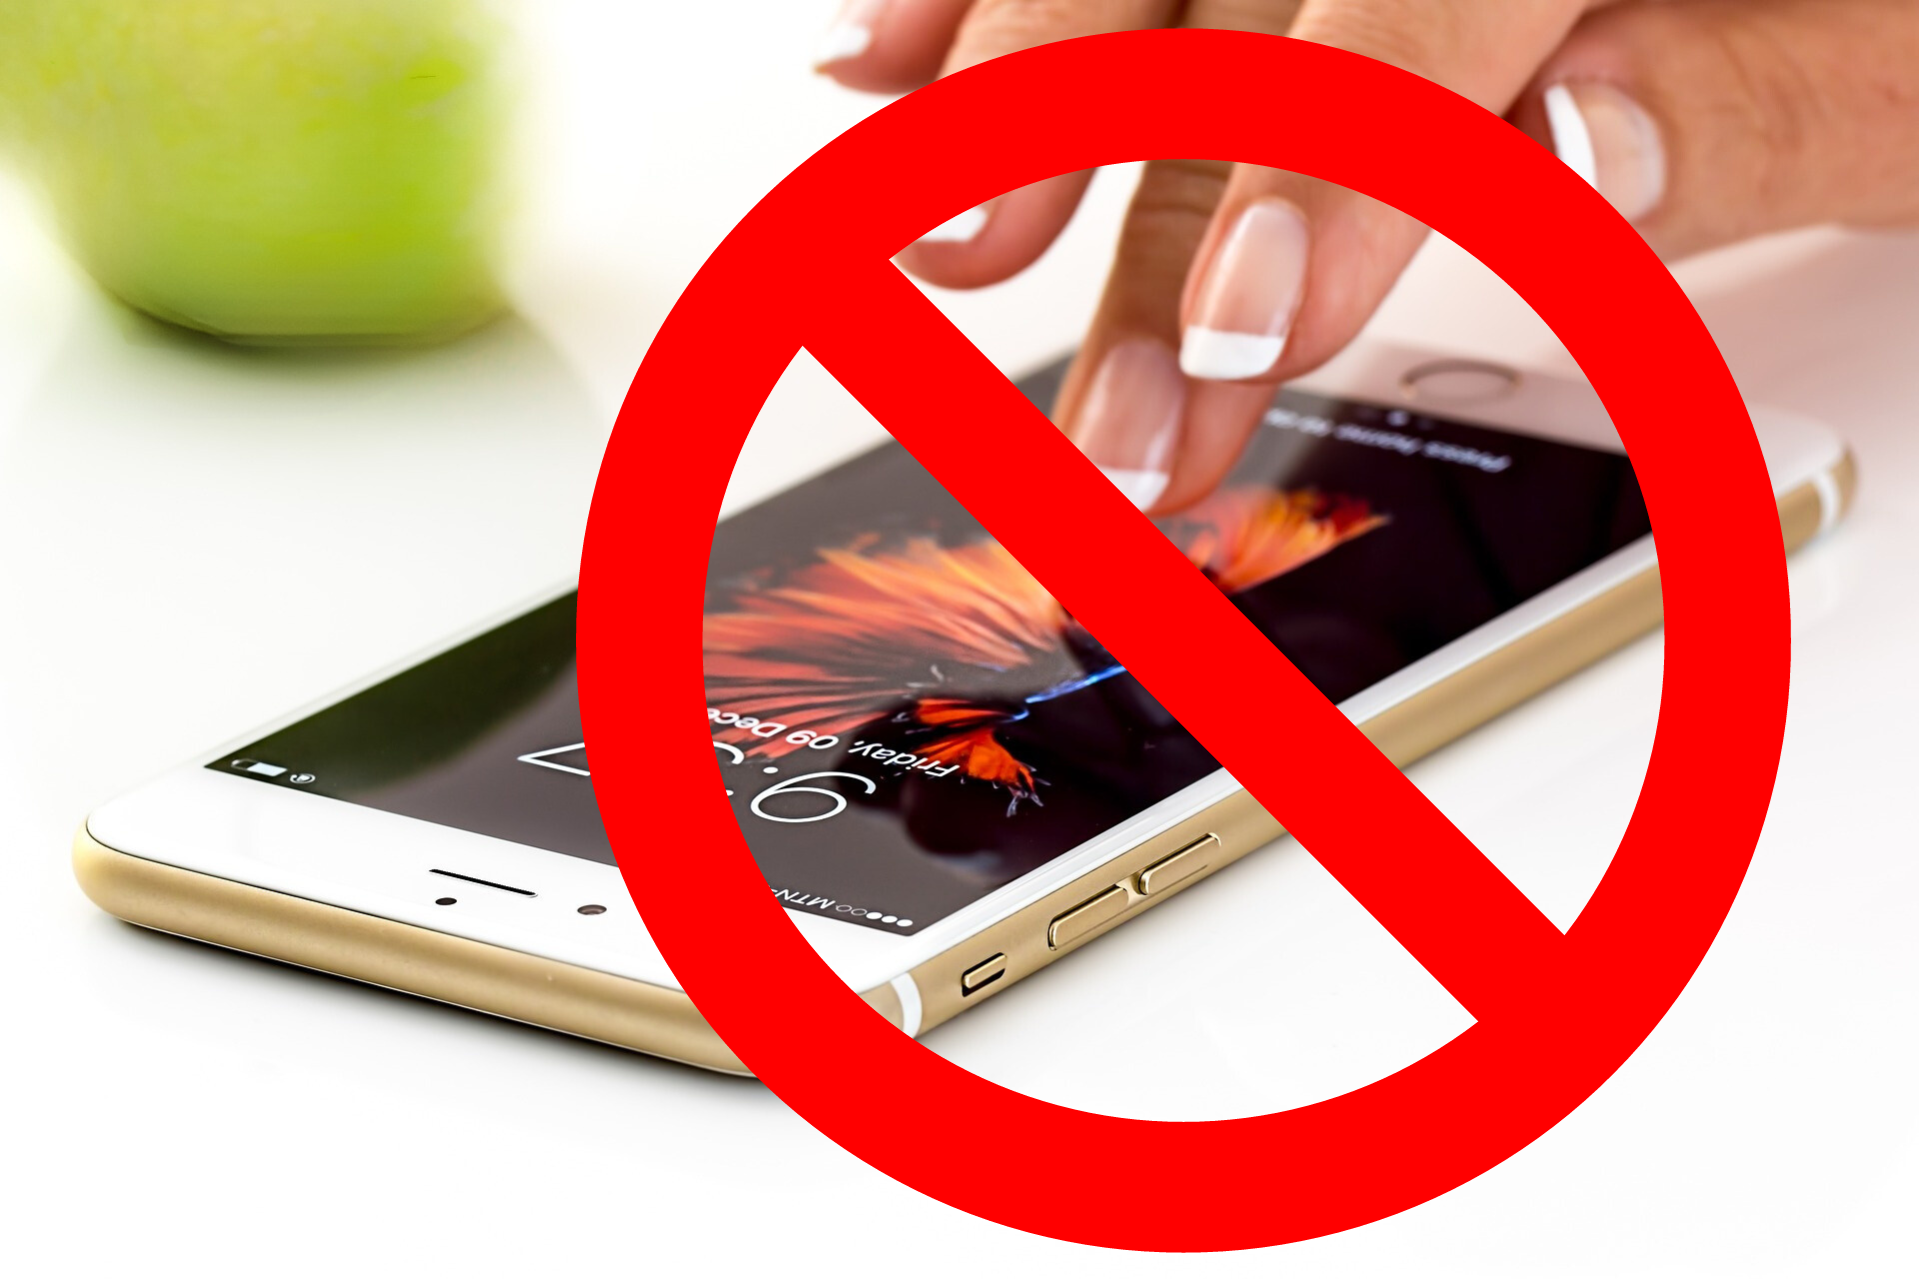
\includegraphics[width=3.42575in,height=3.5in]{./imgSAEB_6_MAT/media/image39.png}
\end{figure}

A reta vertical é orientada para cima e a reta horizontal é orientada
para a direita.

É comum usar as letras $X$ para a primeira e $Y$ para a segunda, e os termos
``coordenada $X$'' e ``coordenada $Y$''. Cada ponto sobre o plano é
representado por uma letra maiúscula, tal como o exemplo, A (valor em $X$, valor em $Y$).

\conteudo{
\noindent Um polígono é uma figura geométrica plana formada por segmentos de reta
que se encontram apenas em suas extremidades. Um polígono é dito convexo
se qualquer segmento de reta que une dois pontos em seu interior estiver
completamente contido em seu interior.

Já um polígono é côncavo se existir pelo menos um segmento de reta que
une dois pontos em seu interior e que não está completamente contido em
seu interior. Em outras palavras, se houver algum ponto no interior do
polígono a partir do qual se possa traçar uma reta que corte uma aresta
do polígono.

%Exemplo de polígono côncavo:

% Tabela
% https://en.wikipedia.org/wiki/Concave\_polygon\#/media/File:Simple\_polygon.svg.
% Acesso em $7$ maio $2023$.

%Exemplo de polígono convexo:

% Tabela
% Disponível em:
% https://en.wikipedia.org/wiki/Convex\_polygon\#/media/File:Pentagon.svg.
% Acesso em $7$ maio $2023$.
}

\conteudo{
\textbf{Fórmula de Euler}\\

\noindent A relação de Euler, quando aplicada a poliedros convexos, estabelece uma
relação fundamental entre o número de vértices, o número de arestas e o
número de faces desses poliedros. Essa relação é conhecida como Fórmula
de Euler para poliedros convexos, e é dada pela seguinte expressão:

$$V - A + F = 2$$

onde, $V$ é o número de vértices do poliedro, $A$ é o número de arestas do
poliedro e $F$ é o número de faces do poliedro.

Essa fórmula estabelece que a soma do número de vértices, o número de
faces e o número de arestas de um poliedro convexo é sempre igual a $2$. É
importante notar que essa fórmula só se aplica a poliedros convexos, ou
seja, aqueles que não possuem nenhuma face côncava ou voltada para
dentro.}

\conteudo{
\noindent \textbf{Elementos de circunferência}\\

\noindent Uma circunferência é uma figura geométrica plana formada por todos os
pontos que estão a uma distância constante, chamada raio, de um ponto
central. Os elementos de uma circunferência são:

\noindent\textit{Centro}\quad é o ponto central da circunferência, que fica equidistante de
todos os pontos da circunferência. O centro é geralmente representado
pela letra O.

\noindent\textit{Raio}\quad é a distância do centro da circunferência até qualquer ponto da
sua circunferência. A letra R é usada para representar o raio.

\noindent\textit{Diâmetro}\quad é uma reta que passa pelo centro da circunferência e que liga
dois pontos opostos da sua circunferência. O diâmetro é igual a duas
vezes o raio. A letra D é usada para representar o diâmetro.

\noindent\textit{Corda}\quad é uma reta que liga dois pontos da circunferência. Uma corda não
necessariamente passa pelo centro da circunferência. Qualquer corda que
passa pelo centro é chamada de diâmetro.

\noindent\textit{Arco}\quad é uma parte da circunferência, limitada por dois pontos. O
comprimento do arco é proporcional ao ângulo central correspondente.

\noindent\textit{Tangente}\quad um ponto em comum com a circunferência.

\noindent\textit{Secante}\quad dois pontos em comum com a circunferência.}

\colorsec{Atividades}

\num{1}  Considere um poliedro convexo. Use a fórmula de Euler para determinar
o número de faces desse poliedro, sabendo que possui $10$ vértices e $20$
arestas.

\reduline{A fórmula de Euler para poliedros convexos é dada por $V - A + F = 2$.
Podemos usar essa fórmula para determinar o número de faces do poliedro
convexo com $V = 10$ e $A = 20$ da seguinte forma: $V - A + F = 2$; $10 - 20 + F = 2$; $F = 12$. Portanto, o número de faces do poliedro convexo é $12$.\hfill}

\num{2}  Uma professora resolver lançar um desafio aos seus alunos, onde deu
aos seus alunos várias coordenadas para colocarem em um plano
cartesiano, qual figura se formou ao ligar todos os pontos
correspondentes?

\begin{escolha}
\item $A (0,5)$
\item $B (-1,2)$
\item $C (-4,2)$
\item $D (-2,0)$
\item $E (-3,-3)$
\item $F (0,1)$
\item $G (3,-3)$
\item $H (2,0)$
\item $I (4,2)$
\item $J (1,2)$
\end{escolha}

\reduline{Ligando os pontos obtém se a figura de uma estrela.\hfill}\linhas{12}

% \begin{figure}
% 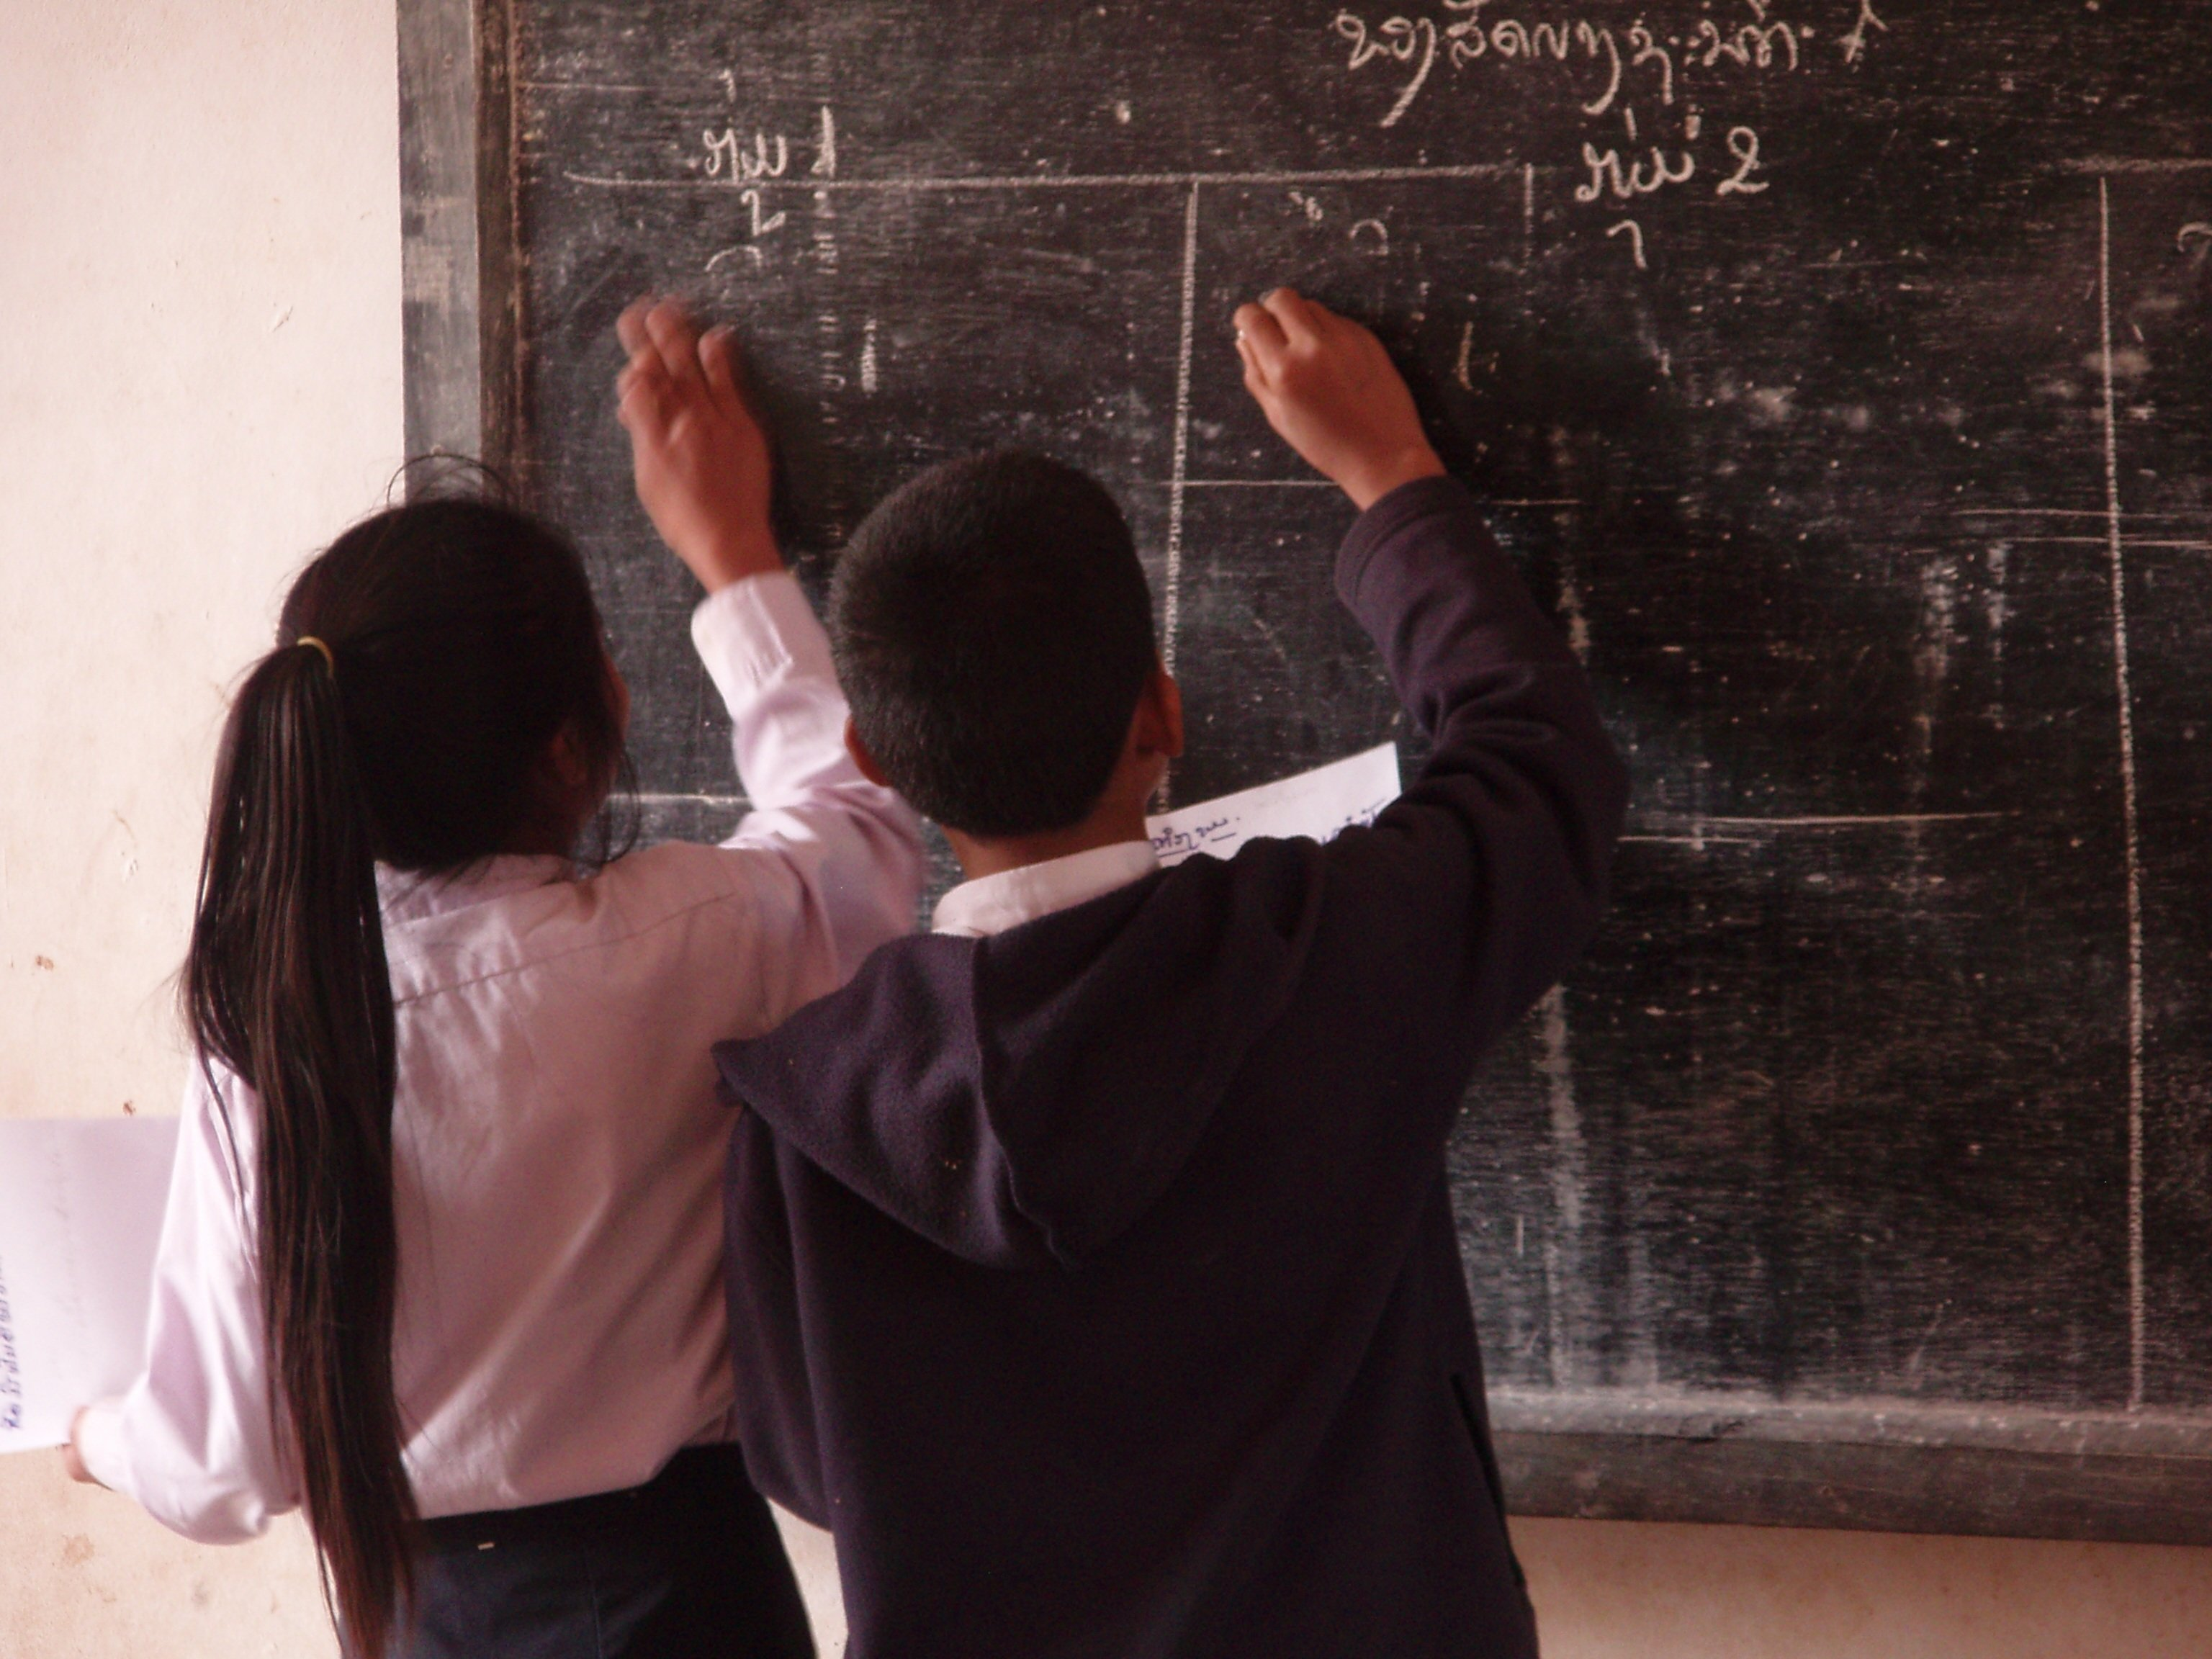
\includegraphics[width=3.85417in,height=3.56597in]{./imgSAEB_6_MAT/media/image45.png}
% \end{figure}

\num{3}  Para realizar o teste físico em determinado concurso da Guarda
municipal, os candidatos devem correr ao redor de uma praça circular
cujo diâmetro mede $90$ m. Uma pessoa que dá $9$ voltas ao redor dessa praça
percorre: (Dado: $π = 3$).

\reduline{$2.430$ m.\hfill}

\num{4}  Quantas arestas tem uma pirâmide quadrangular regular?

\reduline{
Uma pirâmide quadrangular regular tem uma base que é um quadrado, e
quatro faces triangulares congruentes que se encontram em um vértice
comum. Para contar o número de arestas da pirâmide, precisamos contar as
arestas da base (quatro) e as arestas que conectam o vértice da pirâmide
com os vértices da base (quatro). Portanto, a pirâmide quadrangular
regular tem $4 + 4 = 8$ arestas.\hfill}

\num{5}  Na tabela abaixo está transcrito o diâmetro dos planetas do sistema
solar, complete a tabela com os respectivos raios de cada um.

\begin{figure}
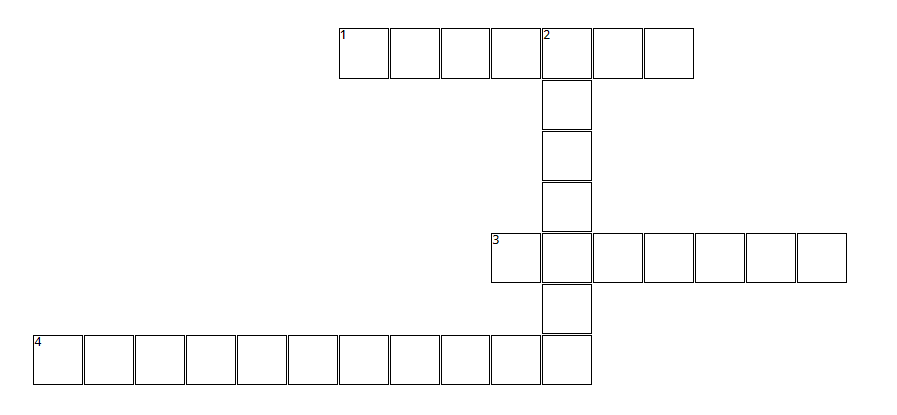
\includegraphics[width=4.05833in,height=4.13212in]{./imgSAEB_6_MAT/media/image48.png}
\end{figure}

\reduline{\hfill}\linhas{4}

% Professor
% Verificar
% 
\includegraphics[width=4.96875in,height=5.22917in]{./imgSAEB_6_MAT/media/image49.png}
% 
\includegraphics[width=1.32083in,height=1.32083in]{./imgSAEB_6_MAT/media/image50.jpeg}

\num{6}  Qual é a medida do maior ângulo formado pelos ponteiros de um relógio
quando ele marca $9$ horas?

\reduline{$270$°.\hfill}

\num{7}  Se os ângulos internos de um polígono regular medem $36$°, então o
número de lados desse polígono é:

\begin{escolha}
\item $10$
\item $17$
\item $12$
\item $13$
\end{escolha}

\reduline{Alternativa A.\hfill}

\num{8}  Lourdes quer Inovar em sua loja de cosméticos e decidiu embalar seus
produtos em caixas de diferentes formatos. Nas imagens abaixo estão as
planificações dessas caixas.

\begin{figure}
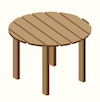
\includegraphics[width=5.90625in,height=2.125in]{./imgSAEB_6_MAT/media/image51.png}
\end{figure}

Quais serão os sólidos geométricos que Lourdes obterá a partir dessas
planificações?

\begin{escolha}
\item Cilindro, prisma de base pentagonal e pirâmide.
\item Cone, prisma de base pentagonal e pirâmide.
\item Cone, tronco de pirâmide e pirâmide.
\item Cilindro, tronco de pirâmide e prisma.
\end{escolha}

\reduline{Alternativa A.\hfill}

%Reproduzir fielmente a imagem descrita acima podendo ser alterado as
%cores, porém não se alterando o conteúdo.

\num{9}  Uma pista de atletismo tem a forma circular e seu diâmetro mede $80$ m.
Um atleta treinando nessa pista deseja correr $10$ km diariamente.
Determine o número mínimo de voltas completas que ele deve dar nessa
pista a cada dia.

\reduline{Ele deve completar no mínimo $40$ voltas completas.\hfill}

\num{10} A Linha poligonal é conhecida por formar os polígonos e são de suma
importância nos estudos da geometria. Para ser identificado como um
polígono, uma figura geométrica plana precisa ser:

\reduline{Fechada e formada por segmentos de retas que não se cruzam.\hfill}

\colorsec{Treino}

\num{1}  Deseja-se pregar uma fita decorativa ao redor da tampa de um pote
redondo. Se o diâmetro da tampa mede $12\,cm$, qual é o comprimento mínimo
que a fita deve ter para dar a volta completa nela?

Considere $π = 3$:

\begin{escolha}
\item $72\,cm$
\item $108\,cm$
\item $35\,cm$
\item $11\,cm$
\end{escolha}

\paragraph{BNCC: EF06MA18 }
% -- Reconhecer, nomear e comparar polígonos, considerando
% lados, vértices e ângulos, e classificá-los em regulares e não
% regulares, tanto em suas representações no plano como em faces de
% poliedros.
% SAEB: Resolver problemas que envolvam relações entre os elementos de uma
% circunferência/círculo (raio, diâmetro, corda, arco, ângulo central,
% ângulo inscrito).

% Gabarito
% Alternativa A: incorreta, pois o aluno pode esquecer que o valor do raio
% é a metade do diâmetro, chegando nesse valor.
% Alternativa B: incorreta, pois ao confundir a fórmula do perímetro da
% circunferência com a fórmula da área da circunferência chegará a esse
% valor.
% Alternativa C: incorreta, pois, ao realizar uma soma ao invés de uma
% multiplicação na fórmula, obterá esse valor.
% Alternativa D: correta, pois ao considerar $\pi = 3$, temos que $2.3.6 = 36\,cm$.

\num{2}  Uma praça possui o formato circular com diâmetro medindo $20$ metros.
Calcule quantos metros quadrados de grama são necessários para preencher
essa área da praça? Considere $π = 3$:

\begin{escolha}
\item $300\,m^2$
\item $60\,m^2$
\item $1200\,m^2$
\item $300\,cm^2$
\end{escolha}

\paragraph{BNCC: EF06MA18 }
% -- Reconhecer, nomear e comparar polígonos, considerando
% lados, vértices e ângulos, e classificá-los em regulares e não
% regulares, tanto em suas representações no plano como em faces de
% poliedros.
% SAEB: Resolver problemas que envolvam relações entre os elementos de uma
% circunferência/círculo (raio, diâmetro, corda, arco, ângulo central,
% ângulo inscrito).

% Gabarito
% Alternativa A: correta, pois, ao calcular a fórmula da área do círculo,
% temos que A= $3\times 10^2 = 300$m²
% Alternativa B: incorreta, pois, ao realizar o cálculo de perímetro da
% circunferência, ao invés do cálculo da área chegaremos a esse valor.
% Alternativa C: incorreta, pois o aluno pode esquecer de trocar o
% diâmetro pelo raio na fórmula e chegará a esse valor.
% Alternativa D: incorreta, pois o aluno pode esquecer de verificar que o
% valor do enunciado se trata de m² e não cm².

\num{3}  Num poliedro convexo, o número de faces é $6$ e o número de vértices é
$8$. Então, o número de arestas desse poliedro é:

(a) $12$

(b) $14$

(c) $2$

(d) $48$

\paragraph{BNCC: EF06MA17 }
% -- Quantificar e estabelecer relações entre o número de
% vértices, faces e arestas de prismas e pirâmides, em função do seu
% polígono da base, para resolver problemas e desenvolver a percepção
% espacial.
% SAEB: Relacionar o número de vértices, faces ou arestas de prismas ou
% pirâmides, em função do seu polígono da base.

% Gabarito
% Alternativa A: correta, pois $V + F = A + 2$; $8 + 6 = A + 2$; $14 = A + 2$; $A = 14 - 2$; $A = 12\,arestas$.
% Alternativa B: incorreta, pois o aluno pode somar todos os números do
% poliedro e chegar a essa conclusão equivocada.
% Alternativa C: incorreta pois o aluno pode realizar uma subtração ao
% invés de utilizar a fórmula.
% Alternativa D: incorreta o aluno pode realizar uma multiplicação ao
% invés de utilizar a fórmula.

\chapter{Triângulos}
\markboth{Módulo 8}{}

\colorsec{Habilidades do SAEB} 
\begin{itemize}
\item Identificar propriedades e relações existentes
entre os elementos de um triângulo (condição de existência, relações de
ordem entre as medidas dos lados e as medidas dos ângulos internos, soma
dos ângulos internos, determinação da medida de um ângulo interno ou
externo).
\item
  Classificar triângulos ou quadriláteros em relação aos lados ou aos
  ângulos internos.
\item
  Identificar retas ou segmentos de retas concorrentes, paralelos ou
  perpendiculares.
\item
  Identificar relações entre ângulos formados por retas paralelas
  cortadas por uma transversal.
\item
  Resolver problemas que envolvam relações entre ângulos formados por
  retas paralelas cortadas por uma transversal, ângulos internos ou
  externos de polígonos ou cevianas (altura, bissetriz, mediana,
  mediatriz) de polígonos.
\item
  Resolver problemas que envolvam relações métricas do triângulo
  retângulo, incluindo o teorema de Pitágoras.
\item
  Resolver problemas que envolvam polígonos semelhantes.
\item
  Resolver problemas que envolvam aplicação das relações de
  proporcionalidade abrangendo retas paralelas cortadas por
  transversais.
\item
  Determinar o ponto médio de um segmento de reta ou a distância entre
  dois pontos quaisquer, dadas as coordenadas desses pontos no plano
  cartesiano.
\end{itemize}

\colorsec{Habilidade da BNCC} 

\begin{itemize}
\item EF06MA19.
\end{itemize}

\conteudo{
\noindent Existem vários tipos de triângulos, e eles podem ser classificados de
acordo com seus lados e ângulos. Abaixo estão os \textbf{principais tipos de
triângulos}:
\begin{itemize}
\item\textit{Triângulo Equilátero}\quad um triângulo equilátero é aquele em que todos os
três lados são iguais. Além disso, todos os ângulos internos desse tipo
de triângulo são iguais a $60$ graus.
\item\textit{Triângulo Isósceles}\quad um triângulo isósceles tem dois lados iguais e um
lado diferente. Os dois ângulos formados pelos lados iguais são iguais
entre si, enquanto o terceiro ângulo é diferente.
\item\textit{Triângulo Escaleno}\quad um triângulo escaleno é aquele em que todos os três
lados são diferentes. Como resultado, os três ângulos internos também
são diferentes.
\item\textit{Triângulo Retângulo}\quad um triângulo retângulo tem um ângulo reto (isto é,
um ângulo de $90$ graus). O lado oposto ao ângulo reto é chamado de
hipotenusa, enquanto os outros dois lados são chamados de catetos. O
teorema de Pitágoras é frequentemente usado para resolver problemas que
envolvem triângulos retângulos.
\item\textit{Triângulo Obtusângulo}\quad um triângulo obtusângulo é aquele em que um dos
ângulos internos é obtuso, ou seja, tem mais de $90$ graus.
\item\textit{Triângulo Acutângulo}\quad um triângulo acutângulo é aquele em que todos os
ângulos internos são agudos, ou seja, têm menos de $90$ graus.
\end{itemize}}

\colorsec{Atividades}

\num{1}  Sabendo que a soma dos ângulos internos de um triângulo
necessariamente é $180$°, complete as figuras abaixo com seus respectivos
ângulos.

\begin{figure}
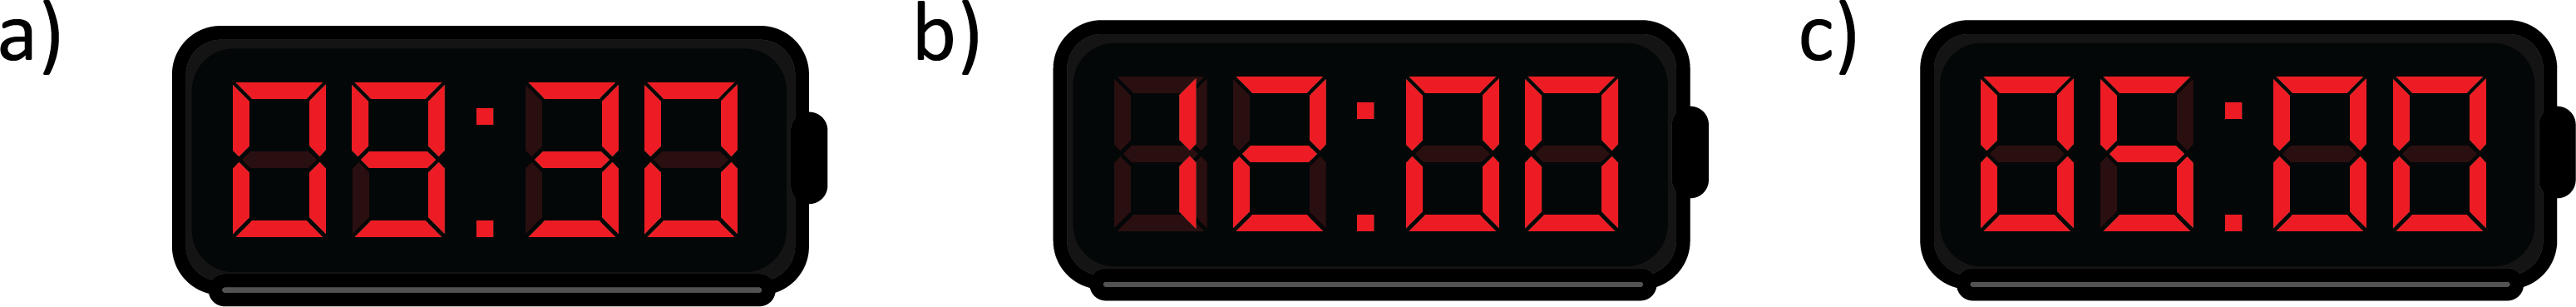
\includegraphics[width=5.90625in,height=3.63542in]{./imgSAEB_6_MAT/media/image52.png}
\end{figure}

\begin{escolha}
\item \reduline{$90$°.\hfill}
\item \reduline{$30$°.\hfill}
\item \reduline{$90$° e $30$°.\hfill}
\item \reduline{$60$°.\hfill}
\item \reduline{$35$°.\hfill}
\item \reduline{$60$°.\hfill}
\end{escolha}

\num{2}  O que é ponto médio?

\reduline{É o ponto central entre dois outros pontos.\hfill}

\num{3}  Com base no mapa abaixo responda com verdadeiro, "V", ou Falso, "F".

\begin{figure}
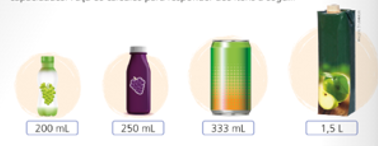
\includegraphics[width=5.47917in,height=2.48958in]{./imgSAEB_6_MAT/media/image53.png}
\end{figure}

\begin{boxlist}
\boxitem[\rosa{V}] As avenidas A e B são paralelas
\boxitem[\rosa{F}] Pode se considerar que a Rua $2$ é paralela a avenida C
\boxitem[\rosa{F}] A avenida C não é paralela a Avenida B
\boxitem[\rosa{V}] a rua $3$ e a rua $2$ são concorrentes
\boxitem[\rosa{V}] A rua $1$ e a rua $3$ não são paralelas
\boxitem[\rosa{F}] A rua $1$ e a Rua $2$ são concorrentes
\end{boxlist}

\num{4}  Angélica decidiu pintar um quadro com as dimensões $100\,cm$ de largura
por $85\,cm$ de altura, com $3$ esferas de cores diferentes. Qual é a área
pintada de cada parte do quadro sabendo que a esfera A tem $60\,cm$ de
diâmetro, a esfera B $20\,cm$ de diâmetro, e a esfera C, $10\,cm$ de diâmetro. Considere π = $3$:

\begin{escolha}
\item Área cinza \reduline{$1200\,cm^2$.\hfill}
\item área azul \reduline{$75\,cm^2$.\hfill}
\item Área rosa \reduline{$2700cm^2$.\hfill}
\item Área verde \reduline{$4525\,cm^2$.\hfill}
\end{escolha}

\begin{figure}
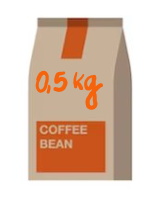
\includegraphics[width=3.70833in,height=3.22917in]{./imgSAEB_6_MAT/media/image54.png}
\end{figure}

\num{5}  Calcule a diagonal de um retângulo de lados $8\,cm$ e $15\,cm$.

\begin{figure}
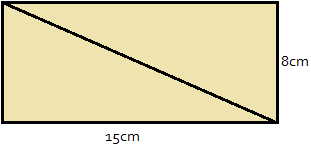
\includegraphics[width=3.24444in,height=1.54653in]{./imgSAEB_6_MAT/media/image55.png}
\end{figure}

\reduline{$A^2= B^2+ C^2$.\hfill}
\reduline{$A^2= 8^2 + 15^2$.\hfill}
\reduline{$A^2= 64 + 225$.\hfill}
\reduline{$A^2= 289$.\hfill}
\reduline{$A = 17$.\hfill}

\num{6}  Um fazendeiro quer construir uma cerca para seu campo, que tem a
forma de um triângulo retângulo. Ele sabe que a distância entre os dois
pontos mais distantes do campo é de $50$ metros e que a distância entre
esses pontos e um terceiro ponto no campo é de $30$ metros. Qual é o
comprimento total da cerca que o fazendeiro precisa comprar?

\reduline{$120\,m$.\hfill}

\num{7}  Um triângulo tem um ângulo interno de $90$ graus, e seus outros dois
ângulos internos são iguais entre si. Além disso, o comprimento de um
dos lados desse triângulo é o dobro do comprimento do outro lado.
Determine os tipos de triângulo possíveis que satisfazem essas
condições.

\reduline{o triângulo pode ser um triângulo retângulo isósceles ou um triângulo
retângulo escaleno.\hfill}

\num{8}  Um triângulo tem dois lados iguais, cada um com $6\,cm$ de comprimento,
e um ângulo diferente, medindo $45$ graus. Classifique esse triângulo de
acordo com seus lados e ângulos.

\reduline{Podemos classificar esse triângulo de duas maneiras: pelos seus lados
e pelos seus ângulos. Pelos lados, esse triângulo tem dois lados iguais, o que significa que é um triângulo isósceles. Pelos ângulos, podemos usar a soma dos ângulos internos de um triângulo,
que é sempre igual a $180$ graus, para encontrar o valor do terceiro
ângulo. Como dois ângulos são iguais a $45$ graus cada, a soma desses
ângulos é $90$ graus. Portanto, o terceiro ângulo é: 180 - $90 = 90$ graus. Esse é um ângulo reto, o que significa que esse triângulo é também um
triângulo retângulo. Assim, podemos concluir que esse triângulo é um triângulo isósceles e
retângulo.\hfill}

\num{9}  Um prédio tem $25$ metros de altura e um poste de luz de $10$ metros de
altura está a uma certa distância da base do prédio. A distância entre a
base do prédio e a base do poste de luz é de $20$ metros. Qual é a
distância entre o topo do poste de luz e o topo do prédio?

\reduline{A distância entre o topo do poste de luz e o topo do prédio é de
aproximadamente $18,72$ m.\hfill}

\num{10}  Um triângulo tem dois lados iguais, com comprimento de $4\,cm$ cada, e
um terceiro lado de $5\,cm$. Qual é o valor do menor ângulo desse
triângulo?

\reduline{O menor ângulo desse triângulo tem um valor de aproximadamente $51,32$
graus.\hfill}

\colorsec{Treino}

\num{1}  Sabendo que (OP) é bissetriz do ângulo AÔB, qual é o valor de x?

\begin{figure}
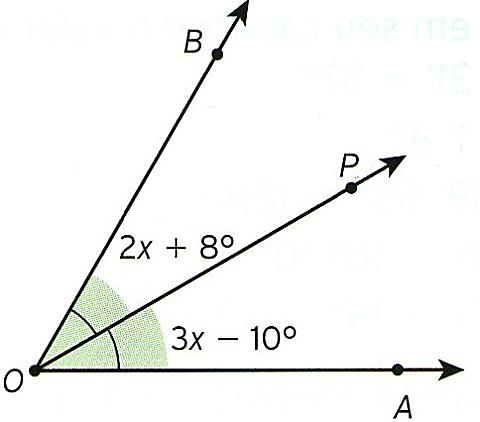
\includegraphics[width=2.17708in,height=1.91619in]{./imgSAEB_6_MAT/media/image62.jpeg}
\end{figure}

\begin{escolha}
\item $-2,5$
\item $13$
\item $18$
\item $45$
\end{escolha}

\paragraph{BNCC: EF06MA19}
%  -- Identificar características dos triângulos e
% classificá-los em relação às medidas dos lados e dos ângulos.
% SAEB: Identificar relações entre ângulos formados por retas paralelas
% cortadas por uma transversal.

% Gabarito
% Alternativa A: incorreta, pois o aluno pode chegar a essa conclusão
% somando os valores literais e dividindo em seguida pelos números
% restantes.
% Alternativa B: incorreta, pois o aluno pode considerar multiplicar os
% valores e dividir após o resultado para chegar a esse valor.
% Alternativa C: correta, pois, Utilizando os conhecimentos sobre
% bissetriz obtemos que as medidas dos Ângulos BÔP e PÔA são iguais, logo $2x+8=3x-10$; $2x-3x= -10 - 8$; $-x = -18$; $x = 18$.
% Alternativa D: incorreta, pois o aluno, pela falta de conhecimento sobre
% bissetriz, pode relembrar que $45$ seja o valor da bissetriz do ângulo
% reto e chegar a essa conclusão mesmo não se tratando de um ângulo reto.

\num{2}  Em um triângulo, se um ângulo mede $90$ graus, quanto mede a soma dos
outros dois ângulos?

\begin{escolha}
\item $60$ graus
\item $90$ graus
\item $100$ graus
\item $180$ graus
\end{escolha}

\paragraph{BNCC: EF06MA19 }
% -- Identificar características dos triângulos e
% classificá-los em relação às medidas dos lados e dos ângulos.
% SAEB: Identificar relações entre ângulos formados por retas paralelas
% cortadas por uma transversal.

% Gabarito
% Alternativa A: incorreta, pois o aluno errou na soma dos ângulos.
% Alternativa B: incorreta, pois o aluno não soube aplicar a soma dos
% ângulos internos.
% Alternativa C: incorreta, pois o aluno não somou $80$º para encontrar o
% resultado correto.
% Alternativa D: correta, pois a soma dos ângulos internos de um triângulo
% é sempre igual a $180$ graus. Se um dos ângulos mede $90$ graus, a soma dos
% outros dois ângulos deve ser igual a $180 - 90 = 90$ graus.

\num{3}  Francisco resolveu fazer um brinquedo de madeira em formato de um
triangulo equilátero para seu filho brincar, sendo assim comprou $3$ peças
de madeira com medidas diferentes, $50\,cm$, $60\,cm$, e $70\,cm$, para que ele
corte apenas $2$ peças, qual a medida que os lados do triangulo
necessariamente devem ter?

\begin{escolha}
\item $70\,cm$
\item $25\,cm$
\item $50\,cm$
\item $55\,cm$
\end{escolha}

\paragraph{BNCC: EF06MA19 }
% -- Identificar características dos triângulos e
% classificá-los em relação às medidas dos lados e dos ângulos.
% SAEB: Identificar relações entre ângulos formados por retas paralelas
% cortadas por uma transversal.

% Gabarito
% Alternativa A: incorreta, pois o aluno pode considerar cortar mais peças
% em relação àquilo que o enunciado recomenda.
% Alternativa B: incorreta, pois o aluno pode considerar cortar mais peças
% em relação àquilo que o enunciado recomenda.
% Alternativa C: correta, pois, para cortar apenas $2$ peças de madeira, o
% brinquedo deverá ser um triangulo de lado $50\,cm$. Como será um triangulo
% equilátero, terá $3$ lados iguais.
% Alternativa D: incorreta, pois o aluno pode considerar cortar mais peças
% em relação àquilo que o enunciado recomenda.

\chapter{A representação do espaço}
\markboth{Módulo 9}{}

\colorsec{Habilidades do SAEB} 
\begin{itemize}
\item Descrever ou esboçar deslocamento de pessoas e/ou
ento de pessoas e/ou de objetos em representações bidimensionais (mapas, croquis etc.),
plantas de ambientes ou vistas, de acordo com condições dadas.
\end{itemize}

\colorsec{Habilidade da BNCC} 
\begin{itemize}
\item EF06MA21
\end{itemize}

\conteudo{
O espaço pode ser representado de diferentes maneiras.

\noindent\textit{Mapa}\quad é uma representação gráfica e simbólica de uma região ou área,
geralmente em escala reduzida, que apresenta informações sobre a
localização, a topografia, a hidrografia, a vegetação, a infraestrutura,
entre outros elementos geográficos e culturais.

\noindent\textit{Planta}\quad é um tipo de mapa que representa a planta baixa ou a vista aérea
de uma construção, edifício, casa, jardim ou terreno, por exemplo. É
utilizada na arquitetura, engenharia civil, urbanismo e paisagismo,
entre outras áreas.

\noindent\textit{Croqui}\quad é um desenho esquemático, geralmente feito à mão livre, que
representa um objeto, uma paisagem, um ambiente ou uma ideia de forma
simplificada e sem escala. É usado em diversos campos, como arquitetura,
design, geografia, artes, entre outros.

\noindent\textit{Escala}\quad é a relação matemática entre as medidas reais e as medidas
representadas em um mapa, planta ou croqui. Ela indica quantas vezes a
distância real é maior do que a distância representada no desenho. Por
exemplo, uma escala de $1$:$1000$ significa que cada $1\,cm$ no mapa representa
$1000$ cm (ou $10$ metros) na realidade. A escala é fundamental para
garantir a precisão e a confiabilidade das informações apresentadas em
um desenho ou mapa.}

\colorsec{Atividades}

\num{1}  Veja abaixo o mapa onde José mora. No mapa, José quer localizar a escola considerando o número e uma letra
qual é a localização da escola?

\begin{figure}
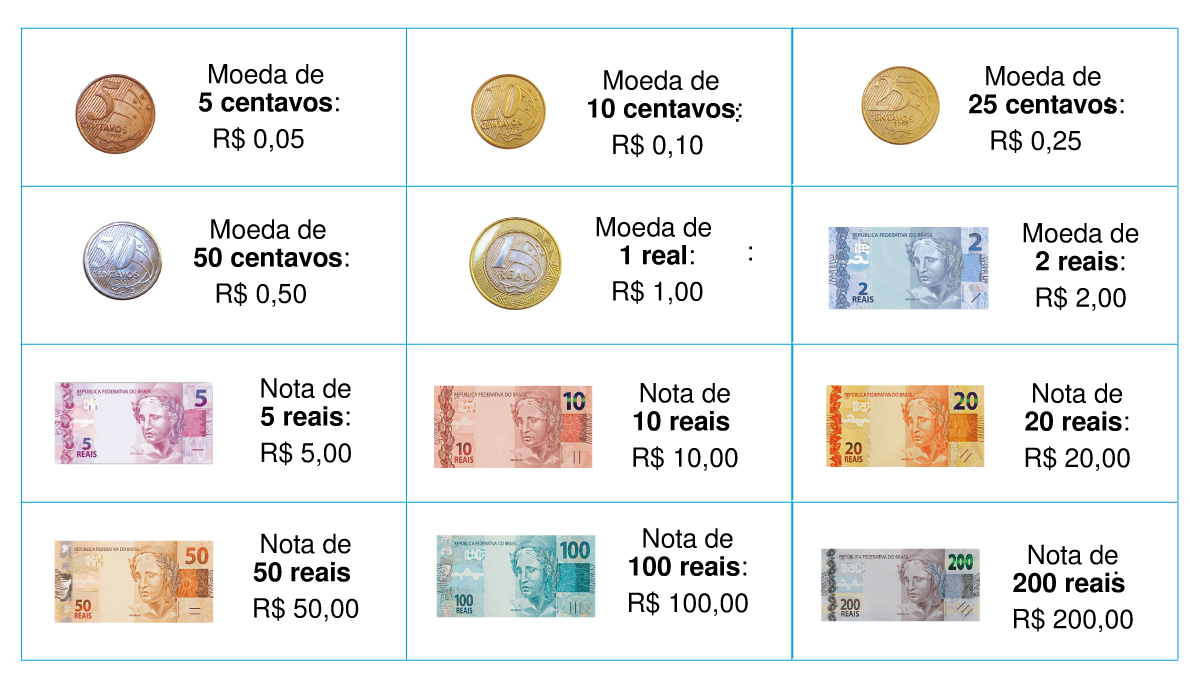
\includegraphics[width=3.86042in,height=3.68611in]{./imgSAEB_6_MAT/media/image64.png}
\end{figure}

\reduline{3, E.\hfill}

\num{2}  Observe abaixo a representação de parte do mapa de uma cidade
planejada. Juca saiu da praça central e orientando se por esse mapa caminhou $3$
quadras na direção leste e depois, $2$ quadras na direção norte diante do
exposto acima, onde Juca parou:

\begin{figure}

\includegraphics[width=3.39535in,height=3.14326in]{./imgSAEB_6_MAT/media/image65.png}
\end{figure}

\reduline{Posto de gasolina.\hfill}

\num{3}  Observe abaixo o mapa do bairro onde Gabriela mora. Gabriela estava na Praça dos Coqueiros e passou na padaria antes de ir
para casa. Qual dos caminhos Gabriela fez para chegar em casa?

\begin{figure}

\includegraphics[width=4.95347in,height=3.13958in]{./imgSAEB_6_MAT/media/image66.png}
\end{figure}

\reduline{Entrou na Rua das Margaridas e virou na Rua dos Cravos.\hfill}

\num{4}  O croqui abaixo mostra um mapa que fornece as indicações para se
chegar à chácara nele indicada. Luna, para chegar à chácara, após fazer o retorno, deve:

\begin{figure}
\includegraphics[width=4.95347in,height=2.04653in]{./imgSAEB_6_MAT/media/image67.png}
\end{figure}

\reduline{Virar à direita, virar à esquerda, entrar na rua $4$.\hfill}

\num{5}  Observe o mapa abaixo. Localizado na Rua Isabel Schimdt, entre a rua Dr.~Antônio Bento e Av.
Adolfo Pinheiro está:

\begin{figure}
\includegraphics[width=5.90625in,height=3.34375in]{./imgSAEB_6_MAT/media/image68.png}
\end{figure}

\reduline{A Santa Casa.\hfill}

\num{6}  A figura abaixo mostra a localização de quatro crianças em relação às
ruas Alegria e Beija-Flor. As demais ruas traçadas são paralelas à Rua
Alegria ou a Rua Beija-flor. A distância entre cada uma das ruas é de
100m.

\begin{figure}
\includegraphics[width=4.19792in,height=2.93056in]{./imgSAEB_6_MAT/media/image69.png}
\end{figure}

\reduline{André está à mesma distância das ruas Alegria e Beija-Flor.\hfill}

\num{7}  Observe o mapa abaixo. Segundo o Mapa, a Praça da Matriz e o Hospital São José se localizam,
respectivamente, nas coordenadas:

\begin{figure}
\includegraphics[width=5.08333in,height=5.71875in]{./imgSAEB_6_MAT/media/image70.png}
\end{figure}

\reduline{(A, $2$) e (A, $4$).\hfill}

\num{8}  Hélio desenhou a planta da casa onde mora. Ela tem dois quartos, uma
sala, uma cozinha e um banheiro. Ao entrar em sua casa pela porta da sala e virar à direita, Hélio está
indo em direção:

\begin{figure}
\includegraphics[width=4.94792in,height=2.46875in]{./imgSAEB_6_MAT/media/image71.png}
\end{figure}

\reduline{Ao quarto $2$.\hfill}

\num{9}  A figura abaixo representa o mapa de um bairro, sendo que cada
quadrado representa um quarteirão, cuja distância entre duas esquinas é
de $100$ m.

\begin{figure}
\includegraphics[width=4.82569in,height=3.77917in]{./imgSAEB_6_MAT/media/image72.png}
\end{figure}

Uma pessoa saiu da esquina indicada pelo ponto P e percorreu o seguinte
percurso:

\begin{itemize}
\item Caminhou $300$ metros na direção Sul;
\item Depois caminhou $200$ metros na direção Leste;
\item E, finalmente, caminhou mais $100$ metros na direção Sul.
\end{itemize}

Ao final desse percurso, essa pessoa chegou na esquina indicada pela
letra: \reduline{Q.\hfill}

\num{10} Bia e Celso estão jogando batalha naval. Em dado momento, só sobrou
um submarino para Bia, na posição descrita na figura abaixo. Para Celso ganhar a partida, é preciso que sua jogada seja:

\begin{figure}
\includegraphics[width=5in,height=3.55208in]{./imgSAEB_6_MAT/media/image73.png}
\end{figure}

\reduline{G2.\hfill}

\colorsec{Treino}

\num{1}  Os retângulos da figura representam cidades. Os números na figura
representam os preços dos bilhetes de comboio entre cidades vizinhas. O
Evandro quer ir da cidade A para a cidade B usando o trajeto mais
barato.

\begin{figure}
\includegraphics[width=5.90625in,height=2.38542in]{./imgSAEB_6_MAT/media/image74.png}
\end{figure}

\noindent Qual é o menor preço que o Pedro tem de pagar para viajar da cidade A
para a cidade B?

\begin{escolha}
\item $80$.
\item $90$
\item $100$.
\item $110$.
\end{escolha}

\paragraph{BNCC: EF06MA21 }
% -- Construir figuras planas semelhantes em situações de
% ampliação e de redução, com o uso de malhas quadriculadas, plano
% cartesiano ou tecnologias digitais.
% SAEB: Descrever ou esboçar deslocamento de pessoas e/ou de objetos em
% representações bidimensionais (mapas, croquis etc.), plantas de
% ambientes ou vistas, de acordo com condições dadas

% Gabarito
% Alternativa A: incorreta, pois o aluno pode esquecer de somar um
% quadrinho e chegar a esse número.
% Alternativa B: correta: pois, é utilizada a rota $20 + 10 + 30 + 20 + 10 = 90$.
% Alternativa C: incorreta, pois o aluno pode considerar seguir por uma
% rota que não seja a mais vantajosa.
% Alternativa D: incorreta, pois o aluno pode considerar seguir por uma
% rota que não seja a mais vantajosa.

\num{2}  No mapa abaixo, encontram-se representadas as ruas do bairro onde
Natasha mora. Natasha informou que mora numa rua entre as avenidas A e B e entre as
ruas do hospital e da locadora. Ela mora na:

\begin{figure}
\includegraphics[width=4.76042in,height=3.42708in]{./imgSAEB_6_MAT/media/image75.png}
\end{figure}

\begin{escolha}
\item Rua $4$
\item Rua $5$.
\item Rua $7$.
\item Rua $9$.
\end{escolha}

\paragraph{BNCC: EF06MA21 }
% -- Construir figuras planas semelhantes em situações de
% ampliação e de redução, com o uso de malhas quadriculadas, plano
% cartesiano ou tecnologias digitais.
% SAEB: Descrever ou esboçar deslocamento de pessoas e/ou de objetos em
% representações bidimensionais (mapas, croquis etc.), plantas de
% ambientes ou vistas, de acordo com condições dadas

% Gabarito
% Alternativa A: correta, pois as coordenadas indicam essa localização.
% Alternativa B: incorreta, pois o aluno pode se perder na condução do
% mapa e chegar a essa conclusão erroneamente.
% Alternativa C: incorreta, pois o aluno pode se perder na condução do
% mapa e chegar a essa conclusão erroneamente.
% Alternativa D: incorreta, pois o aluno pode se perder na condução do
% mapa e chegar a essa conclusão erroneamente.

\num{3}  Qual das seguintes afirmações melhor descreve a diferença entre mapa,
planta e croqui?

\begin{escolha}
\item
  Um mapa é uma representação de uma região ou área, enquanto uma planta
  é um desenho esquemático de uma construção, e um croqui é uma vista
  aérea de uma cidade ou paisagem.
\item
  Um mapa é uma vista aérea de uma cidade ou paisagem, enquanto uma
  planta é uma representação de uma região ou área, e um croqui é um
  desenho esquemático de uma construção.
\item
  Um mapa é um desenho esquemático de uma construção, enquanto uma
  planta é uma representação de uma região ou área, e um croqui é uma
  vista aérea de uma cidade ou paisagem.
\item
  Um mapa, uma planta e um croqui são todos sinônimos e podem ser usados
  de forma intercambiável.
\end{escolha}


\paragraph{BNCC: EF06MA21 }
% -- Construir figuras planas semelhantes em situações de
% ampliação e de redução, com o uso de malhas quadriculadas, plano
% cartesiano ou tecnologias digitais.
% SAEB: Descrever ou esboçar deslocamento de pessoas e/ou de objetos em
% representações bidimensionais (mapas, croquis etc.), plantas de
% ambientes ou vistas, de acordo com condições dadas

% Gabarito
% Alternativa A: correta, pois essa definição está correta.
% Alternativa B: incorreta, pois as primeiras definições estão incorretas.
% Alternativa C: incorreta, pois a definição de planta está incorreta.
% Alternativa D: incorreta, pois há diferenças entre esses conceitos.

\chapter{A leitura de gráficos}
\markboth{Módulo 10}{}

\colorsec{Habilidades do SAEB} 
\begin{itemize}
\item Identificar os indivíduos (universo ou
população-alvo da pesquisa), as variáveis e os tipos de variáveis
(quantitativas ou categóricas) em um conjunto de dados.
\item
  Representar ou associar os dados de uma pesquisa estatística ou de um
  levantamento em listas, tabelas (simples ou de dupla entrada) ou
  gráficos (barras simples ou agrupadas, colunas simples ou agrupadas,
  pictóricos, de linhas, de setores, ou em histograma).
\item
  Inferir a finalidade da realização de uma pesquisa estatística ou de
  um levantamento, dada uma tabela (simples ou de dupla entrada) ou
  gráfico (barras simples ou agrupadas, colunas simples ou agrupadas,
  pictóricos, de linhas, de setores ou em histograma) com os dados dessa
  pesquisa. - Interpretar o significado das medidas de tendência central
  (média aritmética simples, moda e mediana) ou da amplitude.
\item
  Calcular os valores de medidas de tendência central de uma pesquisa
  estatística (média aritmética simples, moda ou mediana).
\item
  Resolver problemas que envolvam dados estatísticos apresentados em
  tabelas (simples ou de dupla entrada) ou gráficos (barras simples ou
  agrupadas, colunas simples ou agrupadas, pictóricos, de linhas, de
  setores ou em histograma).
\item
  Argumentar ou analisar argumentações/conclusões com base nos dados
  apresentados em tabelas (simples ou de dupla entrada) ou gráficos
  (barras simples ou agrupadas, colunas simples ou agrupadas,
  pictóricos, de linhas, de setores ou em histograma).
\item
  Explicar/descrever os passos para a realização de uma pesquisa
  estatística ou de um levantamento.
\end{itemize}

\colorsec{Habilidades da BNCC}
\begin{itemize} 
\item EF06MA31
\item EF06MA32
\end{itemize}

\conteudo{
\noindent\textbf{Tipos de variáveis}\\

\noindent\textit{Variável Quantitativa}\quad São aquelas que podem ser facilmente descritas por números. Exemplos:
\begin{itemize}
\item Quantidade de irmãos, altura, tempo, quantidades de animais de
estimação, etc.
\end{itemize}

\noindent\textit{Variável Qualitativa}\quad são aquelas que não apresentam quantidade, ou seja, não podem ser medidas por números. Exemplos:
\begin{itemize}
\item Tamanhos de roupa (P, M e G), cor dos olhos, nível de
escolaridade, etc...
\end{itemize}
}

\begin{quote}
\noindent\textbf{Tipos de gráficos mais utilizados em estatística}\\

\noindent\textit{Gráfico de colunas ou barras}\\

\begin{figure}
\includegraphics[width=3.71875in,height=2.20833in]{./imgSAEB_6_MAT/media/image77.png}
\end{figure}

\noindent\textit{Gráfico de linhas}\\

% Tabela
%Fazer a figura abaixo nos moldes do projeto.
%Retirar da legenda o nome das emissoras e colocar A, B, C e D.

\begin{figure}
\includegraphics[width=4.1875in,height=2.6875in]{./imgSAEB_6_MAT/media/image79.png}
\end{figure}

\noindent\textit{Gráfico de setores}\\

\begin{figure}
\includegraphics[width=2.88542in,height=2.03125in]{./imgSAEB_6_MAT/media/image80.png}
\end{figure}
\end{quote}

\colorsec{Atividades}

\num{1}  A tabela abaixo mostra o número de passageiros transportados por um
trem em uma certa semana.

% Tabela
\begin{longtable}[]{@{}ll@{}}
\toprule
Dia da Semana & Número de passageiros\tabularnewline
\midrule
\endhead
Segunda & $280$\tabularnewline
Terça & $187$\tabularnewline
Quarta & $211$\tabularnewline
Quinta & $198$\tabularnewline
Sexta & $291$\tabularnewline
Sábado & $110$\tabularnewline
Domingo & $87$\tabularnewline
\bottomrule
\end{longtable}

Em que dia dessa semana o trem transportou mais passageiros?

\reduline{Na sexta-feira.\hfill}

\num{2}  Em uma competição de natação, na prova dos $100$ m livres masculino, os
resultados finais foram os seguintes:

\begin{figure}
\includegraphics[width=3.92708in,height=0.8125in]{./imgSAEB_6_MAT/media/image81.png}
\end{figure}

Qual é a porcentagem de atletas que nadaram em um tempo superior a $46$
segundos?

\reduline{$75\%$ dos nadadores nadam acima dos $46$ segundos.\hfill}

\num{3}  A imagem a seguir mostra um mapa de uma sala de aula representando a
cor favorita de cada aluno. Construa uma tabela indicando a frequência e
o percentual correspondente a cada cor.

\begin{figure}
\includegraphics[width=3.52292in,height=2.45347in]{./imgSAEB_6_MAT/media/image82.png}
\end{figure}

%Paulo: criar tabela com as informações a seguir:

\begin{longtable}[]{@{}lll@{}}
\toprule
Cores & Frequência & Porcentagem\tabularnewline
\midrule
\endhead
Vermelho & $4$ & $13,3$\tabularnewline
Azul & $5$ & $16,7$\tabularnewline
Amarelo & $7$ & $23,3$\tabularnewline
Rosa & $5$ & $16,7$\tabularnewline
Laranja & $9$ & $30,0$\tabularnewline
\bottomrule
\end{longtable}

\reduline{\hfill}\linhas{1}

\num{4}  Um zoológico famoso contém em seu interior o total de $3.200$ animais
que estão separados por classes.

% Tabela
\begin{longtable}[]{@{}ll@{}}
\toprule
Animais no Zoológico &\tabularnewline
\midrule
\endhead
Classes & Quantidade de animais\tabularnewline
Mamíferos & $479$\tabularnewline
Aves & $1620$\tabularnewline
Répteis & $640$\tabularnewline
Anfíbios & $340$\tabularnewline
Invertebrados & $121$\tabularnewline
\bottomrule
\end{longtable}

Observando os dados, calcule:

\begin{escolha}
\item A Porcentagem de mamíferos \reduline{$14,96875\%$.\hfill}
\item A porcentagem de Aves \reduline{$50,625\%$.\hfill}
\item A porcentagem de Répteis \reduline{$20\%$.\hfill}
\item A porcentagem Anfíbios \reduline{$10,625\%$.\hfill}
\item A porcentagem Invertebrados \reduline{$3,78125\%$.\hfill}
\end{escolha}

\num{5}  Leandro decidiu reorganizar suas atividades diárias semanais em uma
tabela, contendo a quantidade de horas de cada atividade.

\begin{figure}
\includegraphics[width=5.90556in,height=2.41638in]{./imgSAEB_6_MAT/media/image83.png}
\end{figure}

Após a reorganização, quantas horas por semana serão destinadas para
atividades escolares?

\reduline{$5·5 + 1·2 = 27$ horas semanais para atividades escolares.\hfill}

\num{6}  O gráfico a seguir mostra a evolução mensal das vendas de certo
produto de julho a novembro de $2021$.

\begin{figure}
\includegraphics[width=3.36458in,height=2.73558in]{./imgSAEB_6_MAT/media/image84.png}
\end{figure}

Sobre as vendas, pode se afirmar que:

\reduline{O mês de outubro foi o mês com mais vendas.\hfill}

\num{7}  Abaixo temos um gráfico de barras. Cada barra se refere a um mês. Os
meses estão marcados no eixo horizontal. O eixo vertical fornece o
número de bicicletas produzidas pela indústria em cada mês.

\begin{figure}
\includegraphics[width=3.875in,height=3.57292in]{./imgSAEB_6_MAT/media/image85.png}
\end{figure}

Observe o gráfico e responda:

\begin{escolha}
\item Qual é o título do gráfico? \reduline{Produção de bicicletas superbike $1$° semestre de $2021$..\hfill}
\item Quantas bicicletas foram produzidas em janeiro? \reduline{$150$.\hfill}
\item E em maio? \reduline{$250$.\hfill}
\item Em que mês a produção de bicicletas foi maior? \reduline{Junho.\hfill}
\end{escolha}

\num{8}  Dona Cleuza é uma grande cozinheira. Ela sabe fazer vários tipos de
doces e salgados. Para organizar sua produção, ela fez uma tabela com as
encomendas da semana.

\begin{figure}
\includegraphics[width=4.88403in,height=2.27917in]{./imgSAEB_6_MAT/media/image86.png}
\end{figure}

Após completar a tabela, responda:

\begin{escolha}
\item Em que dia da semana houve a maior encomenda? \reduline{Terça-feira.\hfill}
\item Em que dia da semana houve a menor encomenda? \reduline{Segunda-feira.\hfill}
\item Na segunda-feira, quantos doces foram encomendados a mais que salgados? \reduline{$12$ doces a mais.\hfill}
\item Na quarta-feira, quantos salgados foram encomendados a mais que doces? \reduline{$111$ Salgados a mais.\hfill}
\end{escolha}

\num{9}  Observe no gráfico abaixo as vendas de uma sorveteria.

\begin{figure}
\includegraphics[width=3.7in,height=2.1in]{./imgSAEB_6_MAT/media/image87.png}
\end{figure}

a) Quantos sorvetes foram vendidos? \reduline{Segunda-feira: $400$; Terça-feira: $300$; Quarta-feira: $200$; Quinta-feira: $300$; Sexta-feira: $500$.\hfill}

b) Quantos sorvetes foram vendidos na sexta-feira a mais que na
quarta-feira? \reduline{$300$.\hfill}

c) Quantos sorvetes foram vendidos na terça-feira e quinta-feira? \reduline{$300$.\hfill}

d) Se na quarta-feira fosse vendido o dobro de sorvete, esse valor seria
maior ou menor que sexta-feira? \reduline{Menor.\hfill}

\begin{figure}
\includegraphics[width=2.51181in,height=2.47708in]{./imgSAEB_6_MAT/media/image88.png}
\end{figure}

\num{10} Uma empresa de cosméticos lançou no mercado $5$ produtos diferentes:
A, B, C, D e E. O gráfico ao lado mostra o resultado de uma pesquisa feita para
verificar a preferência dos consumidores em relação a esses produtos. Se foram entrevistados $2400$ consumidores, podemos afirmar que preferem o
produto A:

\reduline{$600$ consumidores.\hfill}

\colorsec{Treino}

\num{1}  O trenzinho em que $25\%$ dos vagões estão coloridos é:

\begin{figure}
\includegraphics[width=3.46528in,height=2.38403in]{./imgSAEB_6_MAT/media/image89.png}
\end{figure}

\begin{escolha}
\item $1$
\item $2$
\item $3$
\item $4$
\end{escolha}

\paragraph{BNCC: EF06MA31 }
% -- Identificar as variáveis e suas frequências e os
% elementos constitutivos (título, eixos, legendas, fontes e datas) em
% diferentes tipos de gráfico.
% SAEB: Representar ou associar os dados de uma pesquisa estatística ou de
% um levantamento em listas, tabelas (simples ou de dupla entrada) ou
% gráficos (barras simples ou agrupadas, colunas simples ou agrupadas,
% pictóricos, de linhas, de setores, ou em histograma).

% Gabarito
% Alternativa A: correta, pois $25\,\%$ de $8$ é igual a $2$.
% Alternativa B: incorreta, pois o aluno pode contar vagões a mais que não
% estão coloridos e chegar a essa conclusão.
% Alternativa C: incorreta, pois o aluno pode considerar realizar a conta
% sobre o represente de vagões que não estão coloridos.
% Alternativa D: incorreta, pois o aluno pode não compreender o conceito e
% frações e porcentagem e chegar a esse valor erroneamente.

\num{2}  Em um consultório médico, havia $4$ pessoas na sala de espera. O
atendimento da primeira pessoa durou $18$ minutos; o da segunda, $16$
minutos; o da terceira, $14$ minutos; o da quarta, $20$ minutos.

Qual foi o tempo médio de atendimento, por paciente, nesse consultório?

\begin{boxlist}
\boxitem[] $15$ minutos
\boxitem[] $16$ minutos
\boxitem[] $17$ minutos
\boxitem[] $68$ minutos
\end{boxlist}

\paragraph{BNCC: EF06MA32 }
% -- Interpretar e resolver situações que envolvam dados de
% pesquisas sobre contextos ambientais, sustentabilidade, trânsito,
% consumo responsável, entre outros, apresentadas pela mídia em tabelas e
% em diferentes tipos de gráficos e redigir textos escritos com o objetivo
% de sintetizar conclusões.
% SAEB: Interpretar o significado das medidas de tendência central (média
% aritmética simples, moda e mediana) ou da amplitude.

% Gabarito
% Alternativa A: incorreta, pois o aluno pode realizar o cálculo da
% mediana ao invés da media aritmética e chegar a essa conclusão.
% Alternativa b: incorreta, pois o aluno pode conspirar que o tempo esteja
% sendo modificado por uma P.A, de constante de mesmo valor subindo e
% descendo o tempo.
% Alternativa C: correta, pois utilizando a média aritmética $18 + 16 + 14$
% + $20 = 68$; 68/4 = $17$.
% Alternativa D: incorreta, pois o aluno pode somar todos os termos e
% esquecer de dividir chegando a esse valor.

\num{3}  Cada aluno de uma turma com $60$ alunos obteve nota $5$ ou nota $10$ em uma
lista de atividades. Se a média das notas foi $6$, quantos alunos
obtiveram nota $5$?

\begin{escolha}
\item $46$
\item $48$
\item $50$
\item $52$
\end{escolha}

\paragraph{BNCC: EF06MA32 }
% -- Interpretar e resolver situações que envolvam dados de
% pesquisas sobre contextos ambientais, sustentabilidade, trânsito,
% consumo responsável, entre outros, apresentadas pela mídia em tabelas e
% em diferentes tipos de gráficos e redigir textos escritos com o objetivo
% de sintetizar conclusões.
% SAEB: Interpretar o significado das medidas de tendência central (média
% aritmética simples, moda e mediana) ou da amplitude.

% Gabarito
% Alternativa A: incorreta, pois o aluno que não compreender corretamente
% o enunciado pode calcular $2$ notas a menos e chegar a esse resultado.
% Alternativa b: correta, pois o resultado final da média é $48$ alunos.
% Alternativa c: incorreta, pois o aluno que não compreender corretamente
% o enunciado pode calcular $2$ notas a mais e chegar a esse valor.
% Alternativa d: incorreta, pois o aluno que não compreender corretamente
% o enunciado pode calcular $4$ notas a mais e chegar a esse valor.
% erroneamente

\chapter{Grandezas e medidas}
\markboth{Módulo 11}{}

\colorsec{Habilidades do SAEB}

\begin{itemize}
\item
  Resolver problemas que envolvam medidas de grandezas (comprimento,
  massa, tempo, temperatura, capacidade ou volume) em que haja
  conversões entre unidades mais usuais.
\item
  Resolver problemas que envolvam perímetro de figuras planas.
\item
  Resolver problemas que envolvam área de figuras planas.
\item
  Resolver problemas que envolvam volume de prismas retos ou cilindros
  retos.
\end{itemize}

\colorsec{Habilidade da BNCC} 

\begin{itemize}
\item EF06MA24.
\end{itemize}

\conteudo{
\noindent As unidades de medidas de comprimento surgem para padronizar as medidas
de distância. Existem várias unidades de medidas de comprimento. A
utilizada no sistema internacional de unidades é o metro, e seus
múltiplos (quilômetro, hectômetro e decâmetro) e submúltiplos
(decímetro, centímetro milímetro).

Além dessas unidades, existem outras como as que utilizam o corpo como
parâmetro: o palmo, o pé, a polegada. Ainda, há aquelas que não são do
sistema internacional, mas são utilizadas a depender da região ou de
medidas astronômicas, como a légua, a jarda, a milha e o ano-luz.}

\conteudo{
\noindent\textbf{Perímetro}\\

\noindent O perímetro é uma medida que representa a soma das medidas de todos os
lados de uma figura plana. Em outras palavras, é a distância total ao
redor da figura.

O perímetro é uma medida importante para determinar a quantidade de
material necessário para cercar ou contornar uma figura, como no caso da
construção de cercas, muros, jardins, entre outros. Também é útil em
diversas áreas, como em geometria, construção civil, engenharia,
arquitetura, artes, entre outras.

O cálculo do perímetro varia de acordo com a figura geométrica. Para um
triângulo, basta somar as medidas dos três lados; para um quadrado,
basta multiplicar a medida de um dos lados por $4$; para um círculo, o
perímetro é chamado de circunferência e é calculado por meio da fórmula
2πr (sendo r o raio do círculo).}

\conteudo{
\noindent\textbf{Área}\\

\noindent Área é uma medida que quantifica o tamanho de uma superfície plana ou de
uma região delimitada por uma figura geométrica. A área é expressa em
unidades de medida quadradas, como metros quadrados (m²), centímetros
quadrados (cm²), entre outras.

O cálculo da área varia de acordo com a figura geométrica em questão.
Por exemplo, para um retângulo, a área é calculada multiplicando a
medida da base pela medida da altura; para um círculo, a área é
calculada por meio da fórmula πr², sendo r o raio do círculo; para um
triângulo, a área é calculada pela metade do produto da base pela
altura; e assim por diante.}

\conteudo{
\noindent\textbf{Volume}\\

\noindent O volume de um prisma reto pode ser calculado multiplicando a área da
base do prisma pela sua altura.

A área da base é a área da figura geométrica que forma a base do prisma.
Por exemplo, se a base do prisma for um retângulo, a área da base será
calculada multiplicando a medida da base pela medida da altura do
retângulo.

A altura do prisma é a distância entre as bases paralelas do prisma.
Essa medida deve ser perpendicular às bases.}

\begin{quote}
Portanto, a fórmula para calcular o volume de um prisma reto é:

\begin{itemize}
\item V = Ab x h
\end{itemize}

Já o volume de um cilindro reto pode ser calculado multiplicando a área
da base do cilindro pela sua altura. A área da base do cilindro é igual
à área de um círculo, que é dada pela fórmula πr², onde π é a constante
de Pi, e r é o raio do círculo.

Portanto, a fórmula para calcular o volume de um cilindro reto é:
\begin{itemize}
\item V = πr²h
\end{itemize}

Onde: V = volume do cilindro r = raio da base do cilindro h = altura do
cilindro

\noindent\textbf{Importante}\\
\begin{itemize}
\item 1 m³ = $1.000$ Litros
\item 1 cm³ = $1$ mL
\item 1 dm³ = $1$ Litro
\end{itemize}
\end{quote}

\colorsec{Atividades}

\num{1}  Uma lata de tinta, com a forma de um paralelepípedo retangular reto,
tem as dimensões, em centímetros, mostradas na figura abaixo:

\begin{figure}
\includegraphics[width=1.69792in,height=1.88115in]{./imgSAEB_6_MAT/media/image95.png}
\end{figure}

Calcule o volume máximo de tinta que a lata comporta:

\reduline{$23040\,cm$³ de tinta é a capacidade máxima.\hfill}

\num{2}  Um condomínio contém uma cisterna de formato cilíndrico, com $3$ m de
altura e2 m de diâmetro qual o volume de agua máximo que a cisterna
comporta? Utilize $3,0$ como aproximação para pi.

\reduline{O volume máximo que a cisterna comporta é $9$m³.\hfill}\linhas{3}

\num{3}  Em uma empresa, os setores alfa e beta fazem acordos diferentes
relativos à carga horária semanal de trabalho. O setor alfa trabalha $38$
horas por semana, enquanto o setor beta trabalha $44$ horas semanais.
Quantos minutos o setor beta trabalha a mais por semana do que o setor
Alfa? 

\reduline{$360$ minutos.\hfill}\linhas{1}

\num{4} Calcule:

\begin{escolha}
\item A Área de um quadrado de lado $13\,cm$. \reduline{$169\,cm^2$.\hfill}\linhas{2}
\item Perímetro de um quadrado de lado $9\,cm$. \reduline{$36\,cm$.\hfill}\linhas{2}
\item Área de um retângulo de lados $4\,cm$ e $5\,cm$. \reduline{$20\,cm^2$.\hfill}\linhas{2}
\item Perímetro de um retângulo de lados $6\,cm$ e $4\,cm$. \reduline{$20\,cm$.\hfill}\linhas{2}
\item Área de círculo de raio $4\,cm$, considere (π = $3$). \reduline{$48\,cm^2$.\hfill}\linhas{2}
\item Perímetro de um círculo de diâmetro $8\,cm$ (considere π = $3$). \reduline{$24\,cm$.\hfill}\linhas{2}
\end{escolha}

\num{5}  Marina tem um terreno retangular de $3$ m por $6$ m e pretende cercá-lo
com $3$ voltas de arame farpado. Assinale a alternativa que apresenta a
quantidade em metros de arame farpado que ela precisa comprar para fazer
o que pretende.

\reduline{$54$ m.\hfill}\linhas{1}

\num{6}  Observe a temperatura registrada em um mesmo dia e horário em $4$
cidades do mundo.

\begin{figure}
\includegraphics[width=5.03125in,height=1.1875in]{./imgSAEB_6_MAT/media/image96.png}
\end{figure}

Considerando apenas essas $4$ cidades, a diferença entre a maior e a menor
temperatura, em ºC, nesse dia, foi de

\reduline{$50$ ºC.\hfill}\linhas{1}

\num{7}  Orlando resolveu concretar seu quintal de forma que ainda sobrasse
espaço para futuramente a construção de um jardim, fez então um esboço
de como seria a área concretada. Seguindo as medidas do esboço acima qual é a área em m² a ser
concretada?

\begin{figure}
\includegraphics[width=2.66667in,height=1.6914in]{./imgSAEB_6_MAT/media/image97.png}
\end{figure}

\reduline{$164$m².\hfill}\linhas{2}

\num{8}  Uma placa avisa: é proibido som alto entre $22$ horas e $6$ horas.
Durante quantos minutos essa proibição deve ser respeitada?

\reduline{$360$ minutos.\hfill}\linhas{2}

\num{9}  Pretende-se encher completamente um copo com um liquido. O copo tem
formato cilíndrico, e suas medidas são $10\,cm$ de altura e $4\,cm$ de
diâmetro. A quantidade de liquido que cabe no copo é cerca de

(π = $3$).

\reduline{$120$ mL.\hfill}\linhas{2}

\num{10}  A altura de uma vela mede $28\,cm$ e, conforme ela é consumida, a
medida de sua altura diminui $1$ mm a cada minuto.

Quanto tempo levará até a vela ser completamente consumida?

\reduline{$4$ h $40$ min.\hfill}\linhas{2}

\num{11}  Observe as figuras apresentadas a seguir:

\begin{figure}
\includegraphics[width=5.90625in,height=2.51042in]{./imgSAEB_6_MAT/media/image98.png}
\end{figure}

Complete o quadro abaixo contendo o perímetro e área de cada figura.

%Paulo: Criar uma tabela com as informações abaixo:

\begin{longtable}[]{@{}lll@{}}
\toprule
Figura & Área (cm²) & Perímetro (cm)\tabularnewline
\midrule
\endhead
A & ~ & ~\tabularnewline
B & ~ & ~\tabularnewline
C & ~ & ~\tabularnewline
D & ~ & ~\tabularnewline
E & ~ & ~\tabularnewline
\bottomrule
\end{longtable}

% Verificar. % Não tem resposta.

\begin{figure}
\includegraphics[width=3.44792in,height=1.58333in]{./imgSAEB_6_MAT/media/image99.png}
\end{figure}

\colorsec{Treino}

\num{1}  Uma cooperativa agrícola produziu $36$ toneladas de feijão. Toda essa
produção será embalada em sacos de $120\,kg$ antes de ser transportada para
os distribuidores. Quantos sacos de feijão serão obtidos depois de
embalada toda a produção?

\begin{escolha}
\item $300$ sacos
\item $30$ sacos
\item $3$ sacos
\item $3.000$ sacos
\end{escolha}

\paragraph{BNCC: EF06MA24 }
% -- Resolver e elaborar problemas que envolvam as
% grandezas comprimento, massa, tempo, temperatura, área (triângulos e
% retângulos), capacidade e volume (sólidos formados por blocos
% retangulares), sem uso de fórmulas, inseridos, sempre que possível, em
% contextos oriundos de situações reais e/ou relacionadas às outras áreas
% do conhecimento.
% SAEB: Resolver problemas que envolvam medidas de grandezas (comprimento,
% massa, tempo, temperatura, capacidade ou volume) em que haja conversões
% entre unidades mais usuais.

% Gabarito
% Alternativa A: correta, pois realizamos o cálculo de $36.000$ : $120 = 300$
% Alternativa B: incorreta, pois o aluno pode converter erroneamente
% toneladas para\,kg e chegar a esse valor.
% Alternativa C: incorreta, pois o aluno pode converter erroneamente
% toneladas para\,kg e chegar a esse valor.
% Alternativa D: incorreta, pois o aluno pode converter erroneamente
% toneladas para\,kg e chegar a esse valor.

\num{2}  Um copo cheio de água pesa $325\,g$. Se jogarmos metade da água fora, seu
peso cai para $180\,g$. O peso do copo vazio é

\begin{figure}
\includegraphics[width=2.98958in,height=1.38542in]{./imgSAEB_6_MAT/media/image100.png}
\end{figure}

\begin{escolha}
\item $145\,g$
\item $162,5\,g$
\item $35\,g$
\item $180\,g$
\end{escolha}

\paragraph{BNCC: EF06MA24 }
% -- Resolver e elaborar problemas que envolvam as
% grandezas comprimento, massa, tempo, temperatura, área (triângulos e
% retângulos), capacidade e volume (sólidos formados por blocos
% retangulares), sem uso de fórmulas, inseridos, sempre que possível, em
% contextos oriundos de situações reais e/ou relacionadas às outras áreas
% do conhecimento.
% SAEB: Resolver problemas que envolvam medidas de grandezas (comprimento, a)
% massa, tempo, temperatura, capacidade ou volume)
% entre unidades mais usuais.

% Gabarito
% Alternativa A: incorreta, pois o aluno pode realizar a subtração entre
% valores e chegar a esse valor.
% Alternativa B: incorreta, pois o aluno pode simplesmente dividir o valor
% 325 por $2$ e chegar a essa conclusão.
% Alternativa C: correta, pois a operação chega ao valor $35\,g$.
% Alternativa D: incorreta, pois o aluno pode simplesmente ler o enunciado
% e colocar esse valor como correto.

\num{3}  Oito quadrados iguais são colocados lado a lado, formando um
retângulo cujo perímetro é $72\,cm$. A área de cada quadrado que forma o
retângulo é?

\begin{escolha}
\item $16\,cm^2$
\item $72\,cm^2$
\item $64\,cm^2$
\item $128\,cm^2$
\end{escolha}

\paragraph{BNCC: EF06MA24 }
% -- Resolver e elaborar problemas que envolvam as
% grandezas comprimento, massa, tempo, temperatura, área (triângulos e
% retângulos), capacidade e volume (sólidos formados por blocos
% retangulares), sem uso de fórmulas, inseridos, sempre que possível, em
% contextos oriundos de situações reais e/ou relacionadas às outras áreas
% do conhecimento.
% SAEB: Resolver problemas que envolvam medidas de grandezas (comprimento,
% massa, tempo, temperatura, capacidade ou volume) em que haja conversões
% entre unidades mais usuais.

% Gabarito
% Alternativa A: correta, pois a operação matemática a partir da fórmula
% da área chega ao valor $16cm^2$.
% Alternativa B: incorreta, pois o aluno pode considerar que o perímetro e
% a área sejam iguais e chegar a essa conclusão.
% Alternativa C: incorreta, pois o aluno pode erroneamente dividir o
% retângulo em $2$, descobrindo essa área incorretamente.
% Alternativa D: incorreta, pois o aluno pode considerar a área final do
% retângulo ao invés da área de cada quadrado.

\chapter{ Probabilidade}
\markboth{Módulo 12}{}

\colorsec{Habilidade do SAEB}
\begin{itemize}
\item Resolver problemas que envolvam a probabilidade de
ocorrência de um resultado em eventos aleatórios equiprováveis
independentes ou dependentes.
\end{itemize}

\colorsec{Habilidade da BNCC} 
\begin{itemize}
\item EF06MA30
\end{itemize}

\conteudo{
\noindent A probabilidade é uma medida numérica que expressa a chance de um evento
ocorrer. É uma forma de quantificar a incerteza em uma situação. A
probabilidade é expressa como um número entre $0$ e $1$, sendo $0$ a
probabilidade de um evento impossível e $1$ a probabilidade de um evento
certo.

Por exemplo, se lançarmos uma moeda, a probabilidade de que ela caia com
a face ``cara'' para cima é de $0,5$ (ou $50\%$). Isso significa que, em uma
série de lançamentos de moedas, espera-se que a face ``cara'' apareça em
cerca de metade das vezes.

A probabilidade pode ser calculada através da razão entre o número de
eventos favoráveis e o número total de eventos possíveis. Por exemplo,
se lançarmos um dado de seis faces, a probabilidade de que ele caia com
a face $3$ para cima é de $1/6$, pois há apenas uma face com o número $3$ e
seis faces no total.

A probabilidade também pode ser calculada a partir da frequência com que
um evento ocorre em uma série de experimentos. Por exemplo, se jogarmos
um dado várias vezes e o número $3$ aparecer em $20\%$ dos lançamentos,
podemos estimar que a probabilidade de obter o número $3$ em um lançamento
único é de aproximadamente $0,2$.}

\colorsec{Atividades}

\num{1}  Uma moeda é lançada $3$ vezes. Qual a probabilidade de:

\begin{escolha}
\item sair exatamente $1$ cara \reduline{$3/8$.\hfill}
\item sair pelo menos $1$ cara \reduline{$7/8$.\hfill}
\end{escolha}

\num{2}  Dois dados foram lançados. Qual é a probabilidade de a soma dos
pontos obtidos ser:

\begin{escolha}
\item S=8 \reduline{a) $5/36$.\hfill}
\item S\textgreater8 \reduline{b) $5/18$.\hfill}
\end{escolha}

\num{3}  Ronaldo tem $4$ camisetas e $3$ bermudas. De quantas maneiras diferentes
Ronaldo pode se vestir usando sempre uma bermuda e uma camiseta?

\reduline{$12$ maneiras.\hfill}\linhas{1}

\num{4}  Uma urna contém $100$ bolinhas numeradas de $1$ a $100$. Uma bolinha é
escolhida e é observado seu número. Admitindo probabilidades iguais a
1/100 para todos os eventos elementares, qual a probabilidade de:

%Imagem
%https://unsplash.com/pt-br/fotografias/y7kVrSjm7Vw. Acesso em $08$ maio
%2023.
\begin{escolha}
\item Observarmos um múltiplo de $6$ e de $8$ simultaneamente? \reduline{$1/25$.\hfill}
\item Observarmos um múltiplo de $6$ ou de $8$? \reduline{$6/25$.\hfill}
\item Observarmos um número não múltiplo de $5$? \reduline{$4/5$.\hfill}
\end{escolha}

\num{5}  Uma urna contém $6$ bolas pretas, $2$ brancas e $10$ amarelas. Uma bola é
escolhida ao acaso na urna. Qual a probabilidade de:

\begin{escolha}
\item A bola não ser amarela. \reduline{$4$/9.\hfill}
\item A bola ser branca ou preta. \reduline{$4$/9.\hfill}
\item A bola não ser branca, nem amarela. \reduline{$1/3$.\hfill}
\end{escolha}

\num{6}  Num grupo de $500$ estudantes, $80$ estudam Engenharia, $150$ estudam
Economia e $10$ estudam Engenharia e Economia. Se um aluno é escolhido ao
acaso, qual é a probabilidade de que:

\begin{escolha}
\item ele estude somente Engenharia? \reduline{$7/50$.\hfill}
\item ele estude somente Economia? \reduline{$7/25$.\hfill}
\item ele não estude Engenharia nem Economia? \reduline{$14/25$.\hfill}
\item Ele estude Engenharia ou Economia? \reduline{$11/25$.\hfill}
\end{escolha}

%a) $1/50$: não há pergunta para a resposta "A".

\num{7}  De um grupo de $200$ pessoas, $160$ têm fator Rh positivo, $100$ têm sangue
tipo O e $80$ têm fator Rh positivo e sangue tipo O. Se uma dessas pessoas
for selecionada ao acaso, qual a probabilidade de:

\begin{escolha}
\item Seu sangue ter fator Rh positivo? \reduline{$4/5$.\hfill}
\item Seu sangue não ser tipo O? \reduline{$1/2$.\hfill}
\item Seu sangue ter fator Rh positivo ou ser tipo O? \reduline{$9/10$.\hfill}
\end{escolha}

\num{8}  Na loteria são sorteadas $5$ dezenas distintas dentre as dezenas $00$,
01, $02$, $03$, ..., $99$. Um apostador escolhe $10$ dezenas. Determine a
probabilidade dele fazer:

\begin{escolha}
\item Um terno. \reduline{$0,638353\%$.\hfill}
\item Uma quadra. \reduline{$0,025104\%$.\hfill}
\item A quina. \reduline{$0,000335\%$.\hfill}
\end{escolha}

\num{9}  Com os dígitos $1$, $2$, $3$, $4$, $5$ são formados números de $4$ algarismos
distintos. Um deles é escolhido ao acaso. Qual é a probabilidade de ele
ser:

\begin{escolha}
\item Par. \reduline{$2/5$.\hfill}
\item Ímpar. \reduline{$3/5$.\hfill}
\end{escolha}

\num{10} Oito pessoas (entre elas Pedro e Silvia) são dispostas ao acaso numa
fila. Qual a probabilidade de:

\begin{escolha}
\item Pedro e Silvia ficarem juntos? \reduline{$1/4$.\hfill}
\item Pedro e Silvia ficarem separados? \reduline{$3/4$.\hfill}
\end{escolha}

\num{11} Uma urna contém $5$ bolas vermelhas e $3$ brancas. Duas bolas são
extraídas ao acaso, com reposição. Qual é a probabilidade de:

\begin{escolha}
\item Ambas serem vermelhas? \reduline{$25/64$.\hfill}
\item Ambas serem brancas? \reduline{$9/64$.\hfill}
\end{escolha}

\colorsec{Treino}

\num{1}  Na lanchonete, você pode escolher entre $4$ tipos de pães para seu
sanduíche: pão de forma, pão francês, pão sírio e pão preto. Você pode
escolher também $5$ tipos de recheios: mortadela, queijo, presunto, peito
de peru ou peito de frango. De quantas maneiras diferentes você pode
pedir seu sanduíche com apenas um recheio?

\begin{escolha}
\item $20$ maneiras.
\item $9$ maneiras.
\item $1.024$ maneiras.
\item $1$ maneira.
\end{escolha}

\paragraph{BNCC: EF06MA30 }
% -- Calcular a probabilidade de um evento aleatório,
% expressando-a por número racional (forma fracionária, decimal e
% percentual) e comparar esse número com a probabilidade obtida por meio
% de experimentos sucessivos.
% SAEB: Resolver problemas que envolvam a probabilidade de ocorrência de
% um resultado em eventos aleatórios equiprováveis independentes ou
% dependentes.

% Gabarito
% Alternativa A: correta, pois $4 x 5 = 20$ maneiras.
% Alternativa B: incorreta pois, o aluno pode realizar a soma ao invés da
% multiplicação.
% Alternativa C: incorreta, pois o aluno pode realizar a potenciação ao
% invés da multiplicação.
% Alternativa D: incorreta, pois o aluno pode realizar a subtração ao
% invés da multiplicação.

\num{2}  Dona Josefa vende bolas de sorvete em sua casa. Ela oferece $6$ sabores
aos seus clientes: chocolate, uva, morango, creme, limão e flocos.
Geralmente, seus clientes pedem duas bolas. Quantas combinações de duas
bolas são possíveis com esses sabores de sorvete?

\begin{escolha}
\item $1$ combinação
\item $46.656$ combinações
\item $36$ combinações
\item $12$ combinações
\end{escolha}

\paragraph{BNCC: EF06MA30 }
% -- Calcular a probabilidade de um evento aleatório,
% expressando-a por número racional (forma fracionária, decimal e
% percentual) e comparar esse número com a probabilidade obtida por meio
% de experimentos sucessivos.
% SAEB: Resolver problemas que envolvam a probabilidade de ocorrência de
% um resultado em eventos aleatórios equiprováveis independentes ou
% dependentes.

% Gabarito
% Alternativa A: incorreta, pois o aluno pode realizar a soma ao invés da
% multiplicação e chegar a esse resultado.
% Alternativa b: incorreta, pois o aluno pode realizar uma potenciação ao
% invés da multiplicação. 
% Alternativa C: correta, pois são possíveis $36$ combinações.
% Alternativa D: incorreta, pois o aluno pode realizar uma soma ao invés
% da multiplicação.

\num{3}  Suponha que em uma urna haja $10$ bolas numeradas de $1$ a $10$. Qual é a
probabilidade de se retirar uma bola com número par?

\begin{escolha}
\item $0,2$
\item $0,5$
\item $0,6$
\item $0,8$
\end{escolha}

\paragraph{BNCC: EF06MA30 }
% -- Calcular a probabilidade de um evento aleatório,
% expressando-a por número racional (forma fracionária, decimal e
% percentual) e comparar esse número com a probabilidade obtida por meio
% de experimentos sucessivos.
% SAEB: Resolver problemas que envolvam a probabilidade de ocorrência de
% um resultado em eventos aleatórios equiprováveis independentes ou
% dependentes.

% Gabarito
% Alternativa A: incorreta, pois o aluno pode ter considerado apenas dois
% números.
% Alternativa B: correta, pois há cinco números pares entre um total de
% 10.
% Alternativa C: incorreta, incorreta, pois o aluno pode ter considerado
% seis números.
% alternativa D: incorreta, pois incorreta, pois o aluno pode ter
% considerado oito números.

\chapter{Simulado $1$}

\num{1}  O maior cometa já descoberto é o Holmes, que possui $2.251$ km de
diâmetro. Quantas classes possui o número que representa o diâmetro do cometa?

\begin{escolha}
\item $3$
\item $2$
\item $2.251$
\item $4$
\end{escolha}

\paragraph{BNCC: EF06MA01 }
% -- Utilizar números naturais, inteiros, racionais e
% reais, inclusive raiz quadrada, para resolver problemas com valores
% aproximados, utilizando calculadora, mentalmente ou por meio de
% estimativas, com ou sem o uso de tecnologias digitais.
% SAEB: Compor ou decompor números racionais positivos (representação
% decimal finita) na forma aditiva, ou em suas ordens, ou em adições e
% multiplicações.

% Gabarito
% Alternativa A: incorreta, pois, caso o aluno resolva transformar km em
% m, esse seria o valor, mas não é isso que o enunciado pede.
% Alternativa B: correta, pois O número $2.251$ possui $2$ classes e $4$ ordens.
% Alternativa C: incorreta, pois o aluno pode considerar que o numeral
% signifique o valor da classe, o que está incorreto.
% Alternativa D: incorreta, pois o aluno pode confundir classes com
% ordens.

\num{2}  Vilma possui um tabuleiro quadriculado com $12$ quadradinhos de largura
por $12$ quadradinhos de comprimento. Quantos quadradinhos possui o
tabuleiro de Vilma?

\begin{escolha}
\item $1$
\item $24$
\item $124$
\item $144$
\end{escolha}

\paragraph{BNCC: EF06MA06}
% : Resolver e elaborar problemas que envolvam as ideias de
% múltiplo e de divisor.
% SAEB: Calcular o resultado de adições, subtrações, multiplicações ou
% divisões envolvendo número reais.

% Gabarito
% Alternativa A: incorreta, pois o aluno pode realizar uma divisão ao
% invés da multiplicação.
% Alternativa B: incorreta, pois o aluno pode realizar uma soma ao invés
% da multiplicação.
% Alternativa C: incorreta, pois o aluno pode assinalar essa erroneamente
% por conta da semelhança em relação ao resultado correto.
% Alternativa D: correta, pois número de quadradinhos é $12$ ·12 = $144$.

\num{3}  Em um residencial serão plantadas ao lado da rua de comprimento AB.
Elas serão plantadas igualmente espaçadas como se fosse uma reta
numérica conforme a figura:

% Produzir uma figura semelhante a abaixo. Os espaços entre as árvores
% devem ser os mesmos e a quantidade de espaços não pode ser alterada.

\begin{figure}
\includegraphics[width=5in,height=1.19792in]{./imgSAEB_6_MAT/media/image109.png}
\end{figure}

Qual a fração que a distância entre a primeira e a terceira árvores
representa com relação ao tamanho total?

\begin{escolha}
\item 1/4
\item 2/5
\item 1/3
\item 1/5
\end{escolha}

\paragraph{BNCC: EF06MA09}
% -- Resolver e elaborar problemas que envolvam o cálculo da
% fração de uma quantidade e cujo resultado seja um número natural, com e
% sem uso de calculadora.
% SAEB:Representar frações menores ou maiores que a unidade por meio de
% representações pictóricas ou associar frações a representações
% pictóricas.

% Gabarito
% Alternativa A: incorreta, pois o aluno pode visualizar erroneamente o
% número de arvores na figura acima e chegar a essa conclusão
% precipitadamente.
% Alternativa B: correta, pois,como o tamanho total está dividido em $5$
% partes iguais, a fração será $2/5$.
% Alternativa C: incorreta, pois o aluno pode simplesmente considerar
% todas as àrvores e chegar nesse valor.
% Alternativa D: incorreta, pois, ao contar uma árvore a menos, o aluno
% chegaria a esse valor incorretamente.

\num{4}  Um produtor vendeu sua produção no valor de $$R\$1.000,00$$ a um
feirante com $20\%$ de lucro, e este revendeu essas mercadorias com $20\,\%$
de lucro. Sendo assim o valor final da mercadoria foi de:

\begin{escolha}
\item $R\$1.020,00$
\item $R\$1.200,00$
\item $R\$1.400,00$
\item $R\$1.440,00$
\end{escolha}

\paragraph{BNCC: EF06MA13 }
% -- Resolver e elaborar problemas que envolvam
% porcentagens, com base na ideia de proporcionalidade, sem fazer uso da
% ``regra de três'', utilizando estratégias pessoais, cálculo mental e
% calculadora, em contextos de educação financeira, entre outros.
% SAEB: Resolver problemas que envolvam porcentagens, incluindo os que
% lidam com acréscimos e decréscimos simples, aplicação de percentuais
% sucessivos e determinação de taxas percentuais.

% Gabarito
% Alternativa A: incorreta, pois o aluno pode realizar uma soma ao invés
% de calcular a porcentagem e chegar a esse valor.
% Alternativa b: incorreta, pois o aluno pode realizar o cálculo de apenas
% uma parte do enunciado esquecendo o restante.
% Alternativa C: pois, o aluno pode considerar que o mesmo valor dado de
% 20\% para a primeira parte do enunciado seria o mesmo para a segunda, o
% que está equivocado.
% Alternativa D: correta, pois $1.000 x 1,2 x 1,2$ = $$R\$1.440,00$$

\num{5}  Jean foi ao supermercado e gastou $R\$19,00$ comprando seu chocolate
favorito. Se cada unidade do chocolate custa $R\$4,75$, quantos
chocolates Jean comprou?

\begin{escolha}
\item14,25
\item4
\item $23$, $75$
\item90,25
\end{escolha}

\paragraph{BNCC: EF06MA11 }
% -- Resolver e elaborar problemas com números racionais
% positivos na representação decimal, envolvendo as quatro operações
% fundamentais e a potenciação, por meio de estratégias diversas,
% utilizando estimativas e arredondamentos para verificar a razoabilidade
% de respostas, com e sem uso de calculadora.
% SAEB: Resolver problemas de adição, subtração, multiplicação, divisão,
% potenciação ou radiciação envolvendo número reais, inclusive notação
% científica.

% Gabarito
% Alternativa A: incorreta, pois o aluno pode realizar a subtração ao
% invés da divisão.
% Alternativa B: correta, pois 4,75· x = $19$; x = $4$ chocolates.
% Alternativa C: incorreta, pois o aluno pode realizar a soma ao invés da
% divisão.
% Alternativa D: incorreta, pois o aluno pode realizar a multiplicação ao
% invés da divisão.

\num{6}  Fred foi comemorar a promoção que recebeu de seu chefe em uma
pizzaria. Inicialmente resolveram pedir $3$ pizzas e perceberam que o
valor total seria de $R\$135,00$. Se após alguns cálculos resolvessem
comprar $8$ pizzas, o valor que seria pago é de:

\begin{escolha}
\item $R\$45,00$
\item $R\$135,00$
\item $R\$180,00$
\item $R\$360,00$
\end{escolha}

\paragraph{BNCC: EF06MA07 }
% -- Resolver problemas que envolvam expressões numéricas
% com números naturais e com o uso das propriedades das operações.
% SAEB: Resolver problemas de contagem cuja resolução envolva a aplicação
% do princípio multiplicativo.

% Gabarito
% Alternativa A: incorreta, pois esse seria o valor de apenas $1$ pizza.
% Alternativa B: incorreta, pois esse seria o valor de apenas $3$ pizzas.
% Alternativa C: incorreta, pois esse seria o valor de apenas $4$ pizzas.
% Alternativa D: correta, pois Valor de cada pizza: $R\$135,00/3 = R\$
% 45,00$, Valor de $8$ pizzas: $8 x 45,00 = R\$380,00$.

\num{7}  Pelas regras de um processo seletivo, o candidato que será aprovado
será aquele que tirar todas as notas acima de $30$ além disso obtiver o
maior número de notas iguais. As notas de $4$ candidatos foram colocadas
na tabela abaixo:

% %Paulo: Criar uma tabela com as informações abaixo: Candidato Português
% Matemática Direito Informática ----------- ----------- ------------
% --------- ------------- A $33$ $33$ $33$ $34$ B $32$ $39$ $32$ $40$ C $24$ $37$ $40$ $42$ D $36$
% 16 $26$ $40$

Segundo as regras do concurso, o candidato que será aprovado é a
candidato:

\begin{escolha}
\item A
\item B
\item C
\item D
\end{escolha}

\paragraph{BNCC: EF06MA19 }
% -- Resolver problemas que envolvam informações
% apresentadas em gráficos ou tabelas.
% SAEB: Inferir a finalidade da realização de uma pesquisa estatística ou
% de um levantamento, dada uma tabela (simples ou de dupla entrada) ou
% gráfico (barras simples ou agrupadas, colunas simples ou agrupadas,
% pictóricos, de linhas, de setores ou em histograma) com os dados dessa
% pesquisa.

% Gabarito
% Alternativa A: correta, pois, pela análise da tabela percebe-se que o
% candidato A teve todas as notas acima de $30$ e é o que teve mais notas
% iguais. Portanto, o candidato A deverá ser aprovado.
% Alternativa B: incorreta, pois o aluno pode observar erroneamente os
% dados da tabela e chegar a essa conclusão sem fundamentos.
% Alternativa C: incorreta, pois o aluno pode observar erroneamente os
% dados da tabela e chegar a essa conclusão sem fundamentos.
% Alternativa d: incorreta, pois o aluno pode observar erroneamente os
% dados da tabela e chegar a essa conclusão sem fundamentos.

\num{8} Uma escola fez um levantamento sobre a quantidade de alunos em dois
anos do ensino fundamental. Os dados foram apresentados no gráfico
abaixo:

\begin{figure}
\includegraphics[width=3.78125in,height=1.94792in]{./imgSAEB_6_MAT/media/image110.png}
\end{figure}

Após analisar o gráfico, calcule e assinale a alternativa que traz o
número total de alunos do $4$º ano.

\begin{escolha}
\item $60$
\item $86$
\item $62$
\item $55$
\end{escolha}

\paragraph{BNCC: EF06MA19 }
% -- Resolver problemas que envolvam informações
% apresentadas em gráficos ou tabelas.
% SAEB: Representar ou associar os dados de uma pesquisa estatística ou de
% um levantamento em listas, tabelas (simples ou de dupla entrada) ou
% gráficos (barras simples ou agrupadas, colunas simples ou agrupadas,
% pictóricos, de linhas, de setores, ou em histograma).

% Gabarito
% Alternativa A: incorreta, pois o aluno pode considerar o valor da turma
% a como resposta.
% Alternativa B: correta, pois número de alunos do $4$º ano: $32 + 29 + 25 = 86$.
% Alternativa C: incorreta, pois o aluno pode considerar o valor da turma
% a como resposta.
% Alternativa D: incorreta, pois o aluno pode considerar o valor da turma
% a como resposta.

\num{9}  Mateus precisa ir ao dentista essa semana. Escolhendo ao acaso um dia
da semana para ir ao dentista, qual a probabilidade de Mateus escolher
uma segunda-feira ou uma quinta-feira?

\begin{escolha}
\item
  $1/7$
\item
  $2/7$
\item
  $1/5$
\item
  $2/5$
\end{escolha}


\paragraph{BNCC: EF06MA30 }
% -- Calcular a probabilidade de um evento aleatório,
% expressando-a por número racional (forma fracionária, decimal e
% percentual) e comparar esse número com a probabilidade obtida por meio
% de experimentos sucessivos.
% SAEB: Resolver problemas que envolvam a probabilidade de ocorrência de
% um resultado em eventos aleatórios equiprováveis independentes ou
% dependentes.

% Gabarito
% Alternativa A: incorreta, pois o aluno pode considerar um dia ao invés
% das duas incógnitas.
% Alternativa B: pois Dias da semana: $7$; Escolha: $2$; Probabilidade: $2/7$.
% Alternativa C: incorreta, pois o aluno pode considerar um dia do meio da
% semana encontrar erroneamente esse valor.
% Alternativa D: incorreta, pois o aluno pode considerar dois dias do meio
% da semana apenas e encontrar erroneamente esse valor.

\num{10} Uma máquina leva $6$ horas para fazer uma peça. Quantas horas ela
levará para fazer $3$ peças?

\begin{escolha}
\item $9$ horas
\item $2$ horas
\item $18$ horas
\item $216$ horas
\end{escolha}

% SAEB:Resolver problemas que envolvam variação de proporcionalidade
% direta ou inversa entre duas ou mais grandezas, inclusive escalas,
% divisões proporcionais e taxa de variação.

% Gabarito
% Alternativa A: incorreta, poic o aluno pode realizar uma soma ao invés
% de uma razão.
% Alternativa B: incorreta, pois o aluno pode realizar uma divisão ao
% invés de uma razão.
% Alternativa C: correta, pois, como cada máquina faz uma peça a cada $6$
% horas, ao triplicar a quantidade de peças iremos triplicar o tempo.
% Alternativa D: incorreta, pois o aluno pode realizar uma potenciação ao
% invés de uma razão.

\num{11} Um carro percorre $240$ km em $4$ horas. Qual é a velocidade média do
carro?

\begin{escolha}
\item $236\,km/h$
\item $60\,km/h$
\item $244\,km/h$
\item $960\,km/h$
\end{escolha}

% SAEB: Resolver problemas que envolvam variação de proporcionalidade
% direta ou inversa entre duas ou mais grandezas, inclusive escalas,
% divisões proporcionais e taxa de variação.

% Gabarito
% Alternativa A: incorreta, pois o aluno pode realizar uma subtração ao
% invés de uma razão.
% Alternativa B: correta, pois pela razão entre a distância e tempo
% teremos a velocidade.
% Alternativa C: incorreta, pois o aluno pode realizar uma soma ao invés
% de uma razão.
% Alternativa D: incorreta, pois o aluno pode realizar uma potência ao
% invés de uma razão.

\num{12} Escreva o número romano correspondente ao número decimal $1985$.

\begin{escolha}
\item MCMLXXXIII
\item MCMLXXXIV
\item MCMLXXXV
\item MCMLXXXVI
\end{escolha}

\paragraph{BNCC: EF06MA01 }
% -- Comparar, ordenar, ler e escrever números naturais e
% números racionais cuja representação decimal é finita, fazendo uso da
% reta numérica.
% SAEB: Converter uma representação de um número racional positivo para
% outra representação.

Alternativa A: incorreta, pois o aluno pode compreender erroneamente a
numeração romana e seu sistema consequentemente não tendo um fundamento
básico qualquer valor descrito nas alternativas será um valor possível
para que o aluno seja induzido a qualquer resposta.
Alternativa B: incorreta, pois o aluno pode compreender erroneamente a
numeração romana e seu sistema consequentemente não tendo um fundamento
básico qualquer valor descrito nas alternativas será um valor possível
para que o aluno seja induzido a qualquer resposta.
Alternativa C: correta, pois M = $1000$; CM = $900$; LXXX = $80$; V = $5$.
Alternativa D: incorreta, pois o aluno pode compreender erroneamente a
numeração romana e seu sistema consequentemente não tendo um fundamento
básico qualquer valor descrito nas alternativas será um valor possível
para que o aluno seja induzido a qualquer resposta.

\num{13} Uma folha de papel tem $25$ mm de largura. Qual é a medida equivalente
em centímetros?

\begin{escolha}
\item $0,0025\,cm$
\item $0,25\,cm$
\item $2,5\,cm$
\item $25\,cm$
\end{escolha}

\paragraph{BNCC: EF06MA30 }
% -- Utilizar unidades de medida padronizadas para resolver
% problemas que envolvam medidas de comprimento.
% SAEB: Resolver problemas que envolvam medidas de grandezas (comprimento,
% massa, tempo, temperatura, capacidade ou volume) em que haja conversões
% entre unidades mais usuais.

% Gabarito
% Alternativa A: incorreta, pois o aluno pode colocar erroneamente o valor
% de ``zeros'' na expressão obtendo um resultado equivocado.
% Alternativa b: incorreta, pois o aluno pode colocar erroneamente o valor
% de ``zeros'' na expressão obtendo um resultado equivocado.
% Alternativa C: correta, pois 1 cm = $10$ mm, então $25$ mm = $25 / 10 = 2,5\,cm$.
% Alternativa d: incorreta, pois o aluno pode colocar erroneamente o valor
% de ``zeros'' na expressão obtendo um resultado equivocado.

\num{14} Observe a fração $1/2$. Ela pode ser representada pela figura:

\begin{figure}
\includegraphics[width=3.57531in,height=4.10869in]{./imgSAEB_6_MAT/media/image111.png}
\end{figure}

\paragraph{BNCC: EF06MA09 }
% -- Resolver e elaborar problemas que envolvam o cálculo
% da fração de uma quantidade e cujo resultado seja um número natural, com
% e sem uso de calculadora.
% SAEB: Identificar frações equivalentes.

% Gabarito
% Alternativa A: incorreta, pois o aluno não compreendeu o conceito
% correto de $1/2$ (meio ou metade), logo, qualquer alternativa passa a ser
% válida como reposta.
% Alternativa B: incorreta, pois o aluno não compreendeu o conceito
% correto de $1/2$ (meio ou metade), logo, qualquer alternativa passa a ser
% válida como reposta.
% Alternativa C: incorreta, pois o aluno não compreendeu o conceito
% correto de $1/2$ (meio ou metade), logo, qualquer alternativa passa a ser
% válida como reposta.
% Alternativa D: correta, pois a figura representa a fração $1/2$.

\num{15} Observe a figura:

\begin{figure}
\includegraphics[width=3.01693in,height=2.38354in]{./imgSAEB_6_MAT/media/image112.png}
\end{figure}

A vista $3$ pode ser representada por:

\begin{figure}
\includegraphics[width=3.59198in,height=2.82524in]{./imgSAEB_6_MAT/media/image113.png}
\end{figure}

\paragraph{BNCC: EF06MA09 }
% -- Resolver e elaborar problemas que envolvam o cálculo
% da fração de uma quantidade e cujo resultado seja um número natural, com
% e sem uso de calculadora.
% SAEB: Representar frações menores ou maiores que a unidade por meio de
% representações pictóricas ou associar frações a representações
% pictóricas.

% Gabarito
% Alternativa A: incorreta, pois a falta de adaptação a planificações e
% vistas aéreas pode levar ao aluno confusão de figuras chegando a
% assinalar essa alternativa sem compreender realmente o que a figura
% representa.
% Alternativa B: incorreta, pois a falta de adaptação a planificações e
% vistas aéreas pode levar ao aluno confusão de figuras chegando a
% assinalar essa alternativa sem compreender realmente o que a figura
% representa.
% Alternativa C: correta, pois a vista $1$ está representada na alternativa
% A, vista $2$ na alternativa B, vista $3$ na alternativa C e a alternativa D
% não representa nenhuma vista, pois tem uma sequência de $4$ blocos.
% Alternativa D: incorreta, pois a falta de adaptação a planificações e
% vistas aéreas pode levar ao aluno confusão de figuras chegando a
% assinalar essa alternativa sem compreender realmente o que a figura
% representa.

\chapter{Simulado $2$}

\num{1}  Marcos tem três filhos cujas idades foram representadas em números
romanos:

\begin{itemize}
\item
  José tem IX anos de idade
\item
  André, o mais velho, tem XXIII anos
\item
  Joaquim, o mais novo possui VII anos de idade.
\end{itemize}

Sabendo-se que a idade de Marcos é igual a soma das idades de seus
filhos, podemos afirmar que Marcos possui:

\begin{escolha}
\item $30$ anos de idade
\item $35$ anos de idade
\item $40$ anos de idade
\item $45$ anos de idade
\end{escolha}

\paragraph{BNCC: EF06MA01 }
% -- Comparar, ordenar, ler e escrever números naturais e
% números racionais cuja representação decimal é finita, fazendo uso da
% reta numérica.
% SAEB: Escrever números racionais (representação fracionária ou decimal
% finita) em sua representação por algarismos ou em língua materna ou
% associar o registro numérico ao registro em língua materna.

% Alternativa A: incorreta, pois a conversão entre os dois sistemas
% numéricos não foi realizada corretamente
% Alternativa B: incorreta, pois a conversão entre os dois sistemas
% numéricos não foi realizada corretamente.
% Alternativa C: correta, pois X = $10$; XXIII = $23$; VII = $7$; Idade de Marcos: $10 + 23 + 7 = 40$ anos.
% Alternativa D: incorreta, pois a conversão entre os dois sistemas
% numéricos não foi realizada corretamente.

\num{2}  Entre algumas famílias foram distribuídas $240$ cadernos, $576$ lápis, e
1.080 borrachas. A distribuição foi feita de tal modo que o maior número
de famílias fosse contemplado e que cada família recebesse o mesmo
número de lápis, o mesmo número de cadernos e o mesmo número de
borrachas. Nessas condições o número de famílias que recebeu um kit
contendo lápis, borrachas e cadernos foi de:

\begin{escolha}
\item $24$
\item $28$
\item $30$
\item $42$
\end{escolha}

\paragraph{BNCC: EF06MA10 }
% -- Resolver e elaborar problemas que envolvam adição ou
% subtração com números racionais positivos na representação fracionária.
% SAEB: Resolver problemas que envolvam as ideias de múltiplo, divisor,
% máximo divisor comum ou mínimo múltiplo comum.

% Alternativa A: incorreta, pois, ao não ter um conhecimento prévio sobre
% a realização do M.\,D.\,C. como forma de resposta, qualquer alternativa
% passa a ser um resposta viável ao aluno.
% Alternativa B: incorreta, pois, ao não ter um conhecimento prévio sobre
% a realização do M.\,D.\,C. como forma de resposta, qualquer alternativa
% passa a ser um resposta viável ao aluno.
% Alternativa C: correta , pois MDC $(240; 576; 1 080) = 30$ famílias.
% Alternativa D: incorreta, pois, ao não ter um conhecimento prévio sobre
% a realização do M.\,D.\,C. como forma de resposta, qualquer alternativa
% passa a ser um resposta viável ao aluno.

\num{3} Qual é a fração geratriz da dízima periódica $0,666$\ldots?

\begin{escolha}
\item $2/3$
\item $6$/9
\item $7/10$
\item $3/4$
\end{escolha}

%SAEB: Determinar uma fração geratriz para uma dízima periódica.

% Alternativa A: correta, pois a dízima periódica em questão corresponde a
% essa fração.
% Alternativa B: incorreta, pois $6$/9: essa fração pode ser simplificada
% dividindo o numerador e o denominador por $3$, resultando em $2/3$.
% Portanto, essa é uma resposta equivocada.
% Alternativa C: incorreta, pois $7/10$: essa fração não é equivalente a
% 0,666\ldots, que é maior do que $0,7$. Portanto, essa é uma resposta
% incorreta.
% Alternativa D: incorreta, pois $3/4$: essa fração não é equivalente a
% 0,666\ldots, que é menor do que $0,75$. Portanto, essa é uma resposta
% incorreta.

\num{4}  Um círculo tem diâmetro de $8\,cm$. Qual é a medida do ângulo central
correspondente a um arco que mede $4\,cm$?

\begin{escolha}
\item $45$º
\item $60$º
\item $90$º
\item $120$º
\end{escolha}

% SAEB: Resolver problemas que envolvam relações entre os elementos de uma
% circunferência/círculo (raio, diâmetro, corda, arco, ângulo central,
% ângulo inscrito).

% Alternativa A: incorreta, pois $45$º: essa medida é obtida dividindo a
% medida do arco por metade do diâmetro, ou seja, $4$/(8/2) = $1$. Logo, o
% ângulo central correspondente seria de $1 x 180º = 180$º.
% Alternativa B: correta, pois esse é o resultado da operação.
% Alternativa C: incorreta, pois $90$º: essa medida é obtida dividindo a
% medida do arco pelo raio, ou seja, $4/4 = 1$. Logo, o ângulo central
% correspondente seria de $1 x 180º = 180$º.
% Alternativa D: incorreta, pois $120$º: essa medida é obtida dividindo a
% medida do arco por dois terços do diâmetro, ou seja, $4/((2/3) x $8$) =
% 1,5$. Logo, o ângulo central correspondente seria de $1,5 x 180º = 270$º.

\num{5}  Dois produtos químicos A e B são usados em um laboratório. Cada $1\,g$ do
produto A custa $R\$0,06$ e cada $1\,g$ do produto B custa
$R\$0,10$. Se $100\,g$ de uma mistura dos dois produtos custam $R\$7,20$, a
quantidade do produto A contida nesta mistura é:

\begin{escolha}
\item $70\,g$
\item $7,20\,g$
\item $0,60\,g$
\item $0,10\,g$
\end{escolha}

\paragraph{BNCC: EF06MA14 }
% -- Reconhecer que a relação de igualdade matemática não
% se altera ao adicionar, subtrair, multiplicar ou dividir os seus dois
% membros por um mesmo número e utilizar essa noção para determinar
% valores desconhecidos na resolução de problemas.
% SAEB: Resolver problemas que possam ser representados por sistema de
% equações de 1º grau com duas incógnitas.

% Alternativa A: correta, pois X = quantidade do produto A em gramas y = quantidade do produto B em
% gramas; A = Custo do produto A B = Custo do produto B; x + y = $100$\ldots{} (I) x·A + y·B = $7,20$\ldots{} (II); De (I), deduzimos: y = $100$ \textless{} x; Que aplicamos em (II): x·A + (100-x)·B = $7,20$; Substituindo A e B pelos seus custos em reais: x·0,06 +(100-x)·0,10 = 7,20; Multiplicando toda a equação acima por $100$, a fim de tornar inteiros seus coeficientes: $x·6 + (100-x)·10 = 720$; $6x + 1 000 - 10x = 720 -4x =$; $720 - 1000 -4x = -280 x = 70\,gramas$
% Alternativa B: incorreta, pois esse valor não corresponde aos números
% encontrados na solução da expressão.
% Alternativa C: incorreta, pois esse valor não corresponde aos números
% encontrados na solução da expressão.
% Alternativa D: incorreta, pois esse valor não corresponde aos números
% encontrados na solução da expressão.

\num{6}  Para cobrir $840\,m^2$ de um telhado, $14$ operários, que apresentam a
mesma produtividade, gastam $7$ horas. Para cobrir outros $3.360\,m^2$ do
telhado, foram contratados outros $14$ operários, que também possuem a
mesma produtividade individual dos operários anteriores. A previsão de
tempo que esses $12$ operários gastariam para realizar esse trabalho É de

\begin{escolha}
\item $3$ horas e $30$ minutos.
\item $7$ horas.
\item $14$ horas.
\item $18$ horas e $10$ minutos.
\end{escolha}

\paragraph{BNCC: EF06MA14 }
% -- Reconhecer que a relação de igualdade matemática não
% se altera ao adicionar, subtrair, multiplicar ou dividir os seus dois
% membros por um mesmo número e utilizar essa noção para determinar
% valores desconhecidos na resolução de problemas.
% SAEB: Inferir uma equação, inequação polinomial de 1º grau ou um sistema
% de equações de 1º grau com duas incógnitas que modela um problema.

% Alternativa A: incorreta, pois ,ao realizar incorretamente a montagem da
% regra de $3$, o aluno chegará a esse valor incorreto.
% Alternativa B: incorreta, pois, ao realizar incorretamente a
% multiplicação do resultado final por $2$, o aluno chegará a esse resultado
% equivocadamente.
% Alternativa C: correta.
% Alternativa D: incorreta, pois, ao realizar incorretamente a montagem da
% regra de $3$, o aluno chegará a esse valor incorreto.

% \begin{figure}
% \includegraphics[width=2.76042in,height=1.20833in]{./imgSAEB_6_MAT/media/image116.png}
% \end{figure}

\num{7}  As notas de Geografia de $20$ alunos foram colocadas na tabela abaixo:

%Paulo: Criar uma tabela com as informações a seguir:

\begin{longtable}[]{@{}llllllllll@{}}
\toprule
$7,0$ & $5,0$ & $9,0$ & $5,0$ & $8,0$ & $5,0$ & $8,0$ & $9,0$ & $10,0$ &
$8,0$\tabularnewline
\midrule
\endhead
$6,0$ & $6,0$ & $7,0$ & $7,0$ & $7,0$ & $5,0$ & $5,0$ & $5,0$ & $6,0$ & $6,0$\tabularnewline
\bottomrule
\end{longtable}

Quantos alunos obtiveram nota maior ou igual a $7,0$?

\begin{escolha}
\item $8$
\item $10$
\item $9$
\item $11$
\end{escolha}

\paragraph{BNCC: EF06MA19}
% : Resolver problemas que envolvam informações apresentadas
% em gráficos ou tabelas.~
% SAEB: Argumentar ou analisar argumentações/conclusões com base nos dados
% apresentados em tabelas (simples ou de dupla entrada) ou gráficos
% (barras simples ou agrupadas, colunas simples ou agrupadas, pictóricos,
% de linhas, de setores ou em histograma).

% Alternativa A: incorreta, pois, ao visualizar $2$ valores a menos do que
% realmente está na tabela, o aluno chegará a essa conclusão erroneamente.
% Alternativa B: correta, pois entre as notas fornecidas, temos $10$ notas
% maiores ou iguais a $7,0$.
% Alternativa C: incorreta, pois, ao visualizar $1$ valor a menos do que
% realmente está na tabela, o aluno chegará a essa conclusão erroneamente.
% Alternativa D: incorreta, pois, ao visualizar $1$ valor a mais do que
% realmente está na tabela, o aluno chegará a essa conclusão erroneamente.

\num{8}  A biblioteca municipal de uma cidade do interior de São Paulo fez uma
pesquisa sobre a quantidade de livros retiradas pelas pessoas em alguns
determinados meses. Veja o resultado:

Construir um gráfico como esse, mas nos padrões do projeto.

\begin{figure}
\includegraphics[width=5in,height=1.71875in]{./imgSAEB_6_MAT/media/image117.png}
\end{figure}

Pela análise dos dados a razão entre o número de livros retirados em
abril e o número de livros retirados em junho é de:

\begin{escolha}
\item $1/2$
\item $52/51$
\item $51/52$
\item $1$
\end{escolha}

\paragraph{BNCC: EF06MA19}
% SAEB: Inferir a finalidade da realização de uma pesquisa estatística ou
% de um levantamento, dada uma tabela (simples ou de dupla entrada) ou
% gráfico (barras simples ou agrupadas, colunas simples ou agrupadas,
% pictóricos, de linhas, de setores ou em histograma) com os dados dessa
% pesquisa.
%  -- Resolver problemas que envolvam informações
% apresentadas em gráficos ou tabelas.~

% Alternativa A: incorreta, pois o aluno pode considerar $2$ meses e uma
% razão e chegar nessa conclusão.
% Alternativa B: incorreta, pois o aluno pode inverter as razões e chegar
% nessa conclusão.
% Alternativa C: correta, pois $205/210 = 51/52$.
% Alternativa D: incorreta, pois o aluno pode dividir as razões e
% aproximar os valores para $1$ como resposta.

\num{9}  Qual das alternativas abaixo representa a condição de existência de
um triângulo?

\begin{escolha}
\item A soma dos ângulos internos é maior que $360$ graus. 
\item A medida de um
dos ângulos internos é igual a $90$ graus. 
\item A medida do maior lado é
igual a soma das medidas dos outros dois lados. 
\item A medida do menor
lado é igual a metade da medida da hipotenusa.
\end{escolha}

\paragraph{BNCC: EF06MA19 }
% SAEB: Identificar propriedades e relações existentes entre os elementos
% de um triângulo (condição de existência, relações de ordem entre as
% medidas dos lados e as medidas dos ângulos internos, soma dos ângulos
% internos, determinação da medida de um ângulo interno ou externo).
% -- Identificar características dos triângulos e
% classificá-los em relação às medidas dos lados e dos ângulos.

% Alternativa A: incorreta, pois a soma dos ângulos internos de um
% triângulo é igual a $180$ graus.
% Alternativa B: incorreta, pois, embora seja possível ter triângulos com
% um ângulo interno igual a $90$ graus (triângulo retângulo), essa não é uma
% condição necessária para a existência de um triângulo.
% Alternativa C: correta, pois essa é uma regra aplicada aos triângulos.
% Alternativa D: incorreta, pois essa alternativa apresenta uma informação
% contraditória, pois a hipotenusa é o maior lado em um triângulo
% retângulo, portanto não pode ser menor que um dos outros lados. Além
% disso, não há relação definida entre a medida do menor lado e a da
% hipotenusa.

\num{10} Considere um polígono com $7$ lados. É correto afirmar que:

\begin{escolha}
\item É um polígono regular.
\item É um polígono não regular.
\item É um polígono regular ou não regular, dependendo da medida dos seus
lados.
\item É um polígono regular ou não regular, dependendo da medida de seus
ângulos internos.
\end{escolha}

\paragraph{BNCC: EF06MA18}
%  -- Reconhecer, nomear e comparar polígonos, considerando
% lados, vértices e ângulos, e classificá-los em regulares e não
% regulares, tanto em suas representações no plano como em faces de
% poliedros.
% SAEB: Classificar polígonos em regulares e não regulares.

% Alternativa A: é incorreta, pois o polígono não possui lados e ângulos
% congruentes. Alternativa B: correta, pois essa é uma das características
% do polígono. Alternativa C: é incorreta, pois a medida dos lados não
% influencia na classificação do polígono como regular ou não regular.
% Alternativa D: é incorreta, pois mesmo que os ângulos internos do
% polígono sejam congruentes, ainda assim é impossível que seus lados
% sejam congruentes.

\num{11} Considere três retas paralelas cortadas por uma transversal,
formando oito ângulos. Quantos pares de ângulos são correspondentes?

\begin{escolha}
\item $2$
\item $4$
\item $6$
\item $8$
\end{escolha}

\paragraph{BNCC: EF06MA19}
% SAEB: Identificar relações entre ângulos formados por retas paralelas
% cortadas por uma transversal.
%  -- Identificar características dos triângulos e
% classificá-los em relação às medidas dos lados e dos ângulos.

% Alternativa A: incorreta, pois a alternativa afirma que existem apenas
% dois pares de ângulos correspondentes, o que está errado. Alternativa B:
% incorreta, pois a alternativa afirma que existem quatro pares de ângulos
% correspondentes, o que corresponde ao número de pares de ângulos
% correspondentes formados por duas retas paralelas cortadas por uma
% transversal, não por três retas paralelas. Alternativa C: correta, pois,
% quando uma transversal corta duas retas paralelas, cada par de ângulos
% correspondentes possui medidas iguais. Nesse caso, existem quatro pares
% de ângulos correspondentes (ângulos $1$ e $5$, $2$ e $6$, $3$ e $7$, $4$ e $8$). A
% alternativa D: incorreta, pois a alternativa afirma que existem oito
% pares de ângulos correspondentes, o que está errado.

\num{12} Qual a forma correta de escrever o número $49$ em numeração romana?

\begin{escolha}
\item XLVIX
\item LIXV
\item XLIX
\item XLIVIX
\end{escolha}

\paragraph{BNCC: EF06MA01 }
% SAEB: Comparar ou ordenar números reais, com ou sem suporte da reta
% numérica, ou aproximar número reais para múltiplos de potência de $10$
% mais próxima.
% -- Comparar, ordenar, ler e escrever números naturais e
% números racionais cuja representação decimal é finita, fazendo uso da
% reta numérica.

% Alternativa A: incorreta, o aluno pode chegar a essa conclusão
% esquecendo que que no sistema romano são apenas em casos específicos de
% impossibilidade de colocar mais de $3$ símbolos iguais para representar o
% mesmo número para inserir um número antes de outro representando uma
% subtração momentânea.
% Alternativa B: incorreta, o aluno pode chegar a essa conclusão
% esquecendo que que no sistema romano são apenas em casos específicos de
% impossibilidade de colocar mais de $3$ símbolos iguais para representar o
% mesmo número para inserir um número antes de outro representando uma
% subtração momentânea.
% Alternativa C: correta, pois 40 = XL; 9 = IX; XLIX = $40 + 9 = 49$
% Alternativa D: incorreta, pois o aluno pode chegar a essa conclusão
% esquecendo que que no sistema romano são apenas em casos específicos de
% impossibilidade de colocar mais de $3$ símbolos iguais para representar o
% mesmo número para inserir um número antes de outro representando uma
% subtração momentânea.

\num{13} Um prisma reto tem base quadrada com lado medindo $5\,cm$ e altura
medindo $8\,cm$. Qual é o seu volume?

\begin{escolha}
\item $20\,cm$³
\item $40\,cm$³
\item $100\,cm$³
\item $200\,cm$³
\end{escolha}

\paragraph{BNCC: EF06MA24 }
% SAEB: Resolver problemas que envolvam volume de prismas retos ou
% cilindros retos.
% -- Resolver e elaborar problemas que envolvam as
% grandezas comprimento, massa, tempo, temperatura, área (triângulos e
% retângulos), capacidade e volume (sólidos formados por blocos
% retangulares), sem uso de fórmulas, inseridos, sempre que possível, em
% contextos oriundos de situações reais e/ou relacionadas às outras áreas
% do conhecimento.

% Alternativa A: incorreta, pois esta alternativa corresponde ao cálculo
% do volume de um cubo cujo lado mede $2,5\,cm$, que não é o caso do prisma
% em questão.
% Alternativa B: incorreta, esta alternativa corresponde ao cálculo do
% volume de um prisma retangular com base de $5\,cm$ x $4\,cm$ e altura de $2\,cm$,
% que não é o caso do prisma em questão.
% Alternativa C: incorreta, pois esta alternativa corresponde ao cálculo
% do volume de um prisma triangular com base de $10\,cm^2$ e altura de $10\,cm$,
% que não é o caso do prisma em questão.
% Alternativa D: correta, pois a fórmula para o cálculo do volume de um
% prisma reto é dada por V = Ab x h, em que Ab é a área da base e h é a
% altura. No caso deste prisma, a base é um quadrado, cuja área é dada por
% Ab = lado². Portanto, Ab = $5^2 = 25\,cm^2$. Substituindo os valores na
% fórmula, temos: V = $25\,cm^2$ x $8\,cm$ = $200\,cm$³.

\num{14} Em uma pesquisa sobre a altura de $10$ estudantes de uma turma, os
dados obtidos foram: $1,45\,m$; $1,50\,m$; $1,60\,m$; $1,70\,m$; $1,75\,m$; $1,80\,m$;
1,85 m; $1,90\,m$; $1,95\,m$; $2,00$ m. Qual é a média aritmética simples das
alturas dos estudantes?

\begin{escolha}
\item $1,50\,m$
\item $1,75\,m$
\item $1,85\,m$
\item $1,90\,m$
\end{escolha}

\paragraph{BNCC: EF06MA32 }
% SAEB: Calcular os valores de medidas de tendência central de uma
% pesquisa estatística (média aritmética simples, moda ou mediana).
% -- Interpretar e resolver situações que envolvam dados de
% pesquisas sobre contextos ambientais, sustentabilidade, trânsito,
% consumo responsável, entre outros, apresentadas pela mídia em tabelas e
% em diferentes tipos de gráficos e redigir textos escritos com o objetivo
% de sintetizar conclusões.

% Alternativa A: incorreta, pois a média aritmética simples não é a menor
% altura nem a média entre a menor e a maior altura.
% Alternativa B: incorreta, pois a soma das alturas é maior que $17,5$ (10 x
% 1,75), portanto a média aritmética simples não pode ser menor que $1,75$.
% Alternativa C: correta, pois A média aritmética simples é obtida pela
% soma de todos os valores e divisão pelo número total de elementos.
% Portanto, somando as alturas dos $10$ estudantes, temos: $1,45 + 1,50$ +
% 1,60 + $1,70 + 1,75 + 1,80 + 1,85 + 1,90 + 1,95 + 2,00 = 18,50$ Dividindo
% esse valor por $10$, temos a média aritmética simples: $18,50 / 10 = 1,85$.
% Alternativa D: incorreta, pois A média aritmética simples é menor que a
% maior altura (2,00 m) e maior que a menor altura (1,45 m), portanto a
% alternativa d) é uma possibilidade, mas não é a resposta correta, pois a
% média aritmética simples não é a média entre a menor e a maior altura.

\num{15} Qual é a área de um retângulo de base $5\,cm$ e altura $8\,cm$?

\begin{escolha}
\item
  $13cm^2$
\item
  $35cm^2$
\item
  $40cm^2$
\item
  $56cm^2$
\end{escolha}

\paragraph{BNCC: EF06MA24 }
% SAEB: Resolver problemas que envolvam área de figuras planas.
% -- Resolver e elaborar problemas que envolvam as
% grandezas comprimento, massa, tempo, temperatura, área (triângulos e
% retângulos), capacidade e volume (sólidos formados por blocos
% retangulares), sem uso de fórmulas, inseridos, sempre que possível, em
% contextos oriundos de situações reais e/ou relacionadas às outras áreas
% do conhecimento.

% Alternativa A: incorreta, pois provavelmente houve uma confusão com os
% valores da base e da altura.
% Alternativa B: incorreta, pois o valor encontrado é menor que o produto
% dos valores da base e altura.
% Alternativa C: correta, pois a área de um retângulo é dada pelo produto
% da base pela altura, ou seja: Área = Base x Altura; Substituindo os valores dados na questão, temos: Área = $5\,cm$ x $8\,cm$ Área = $40cm^2$.
% Alternativa D: incorreta, pois o valor encontrado é maior que o produto
% dos valores da base e altura.

\chapter{Simulado $3$}

\num{1}  Qual dos seguintes números é irracional?

\begin{escolha}
\item $0.5$
\item $2/3$
\item raiz quadrada de $25$
\item pi (π)
\end{escolha}

\paragraph{BNCC: EF06MA01 }
% -- Comparar, ordenar, ler e escrever números naturais e
% números racionais cuja representação decimal é finita, fazendo uso da
% reta numérica.
% SAEB: Identificar números racionais ou irracionais.

% Alternativa A: incorreta, pois $0.5$ é um número racional, podendo ser
% expresso como a fração $1/2$. Alternativa B: incorreta, pois $2/3$ é um
% número racional, já que é uma fração. Alternativa C: incorreta, pois a
% raiz quadrada de $25$ é um número inteiro. Alternativa D: correta, pois pi
% (π) é um número irracional, já que não pode ser expresso como uma fração
% finita ou decimal exata. Ele tem uma representação decimal infinita e
% não periódica, o que significa que não há um padrão repetido na
% sequência de seus dígitos.

\num{2}  Amanda abastece seu veículo a cada $5$ dias, Carlos a cada $2$ dias.
Paulo vai abastecer seu veículo sempre aos sábados e em nenhum outro
dia. Se no dia $28$ de outubro os três abasteceram seus veículos, daqui a
quantos dias eles abastecerão, novamente, no mesmo dia?

\begin{escolha}
\item $31$ dias
\item $25$ dias
\item $70$ dias
\item esse evento nunca mais acontecerá.
\end{escolha}

\paragraph{BNCC: EF06MA05 }
% SAEB: Identificar um número natural como primo, composto,
% ``múltiplo/fator de'' ou ``divisor de'' ou identificar a decomposição de
% um número natural em fatores primos ou relacionar as propriedades
% aritméticas (primo, composto, ``múltiplo/fator de'' ou ``divisor de'')
% de um número natural à sua decomposição em fatores primos.

% -- Classificar números naturais em primos e compostos,
% estabelecer relações entre números, expressas pelos termos ``é múltiplo
% de'', ``é divisor de'', ``é fator de'', e estabelecer, por meio de
% investigações, critérios de divisibilidade por $2$, $3$, $4$, $5$, $6$, $8$, $9$, $10$,
% 100 e $1000$.

% Alternativa A: incorreta, pois, por questão de semelhança, o aluno pode
% considerar que as $3$ pessoas citadas no enunciado abastecerão sempre no
% mesmo dia $28$ de todo mês.
% Alternativa B: incorreta, pois o aluno pode realizar uma soma dos dias
% ao invés de realizar o M.\,M.\,C.
% Alternativa C: correta, pois MMC(5;7,2) = $70$. 
% Alternativa D: incorreta, pois o aluno pode confundir M.\,M.\,C. por M.\,D.\,C.

\num{3} Calcule o valor da expressão: $3^2$ + raiz quadrada de $16$.

\begin{escolha}
\item $13$
\item $11$
\item $7$
\item $10$
\end{escolha}

\paragraph{BNCC: EF06MA11 }
% SAEB: Calcular o resultado de potenciação ou radiciação envolvendo
% números reais.
% -- Resolver e elaborar problemas com números racionais
% positivos na representação decimal, envolvendo as quatro operações
% fundamentais e a potenciação, por meio de estratégias diversas,
% utilizando estimativas e arredondamentos para verificar a razoabilidade
% de respostas, com e sem uso de calculadora.

% Alternativa A: incorreta, pois a resolução da expressão não corresponde
% a esse resultado.
% Alternativa B: incorreta, pois a resolução da expressão não corresponde
% a esse resultado.
% Alternativa C: incorreta, pois a resolução da expressão não corresponde
% a esse resultado.
% Alternativa D: correta pois $3^2$ significa $3$ elevado ao quadrado, ou seja,
% 3 x $3 = 9$. A raiz quadrada de $16$ é $4$. Assim, a expressão pode ser
% reescrita como $9 + 4 = 13$.

\num{4}  O número $17$ é classificado como\ldots{}

\begin{escolha}
\item
  Primo.
\item
  Composto.
\item
  Múltiplo de $3$.
\item
  Divisor de $64$.
\end{escolha}

\paragraph{BNCC: EF06MA05 }
% SAEB:Identificar um número natural como primo, composto,
% ``múltiplo/fator de'' ou ``divisor de'' ou identificar a decomposição de
% um número natural em fatores primos ou relacionar as propriedades
% aritméticas (primo, composto, ``múltiplo/fator de'' ou ``divisor de'')
% de um número natural à sua decomposição em fatores primos.
% -- Classificar números naturais em primos e compostos,
% estabelecer relações entre números, expressas pelos termos ``é múltiplo
% de'', ``é divisor de'', ``é fator de'', e estabelecer, por meio de
% investigações, critérios de divisibilidade por $2$, $3$, $4$, $5$, $6$, $8$, $9$, $10$,
% 100 e $1000$.
% EF06MA14: Resolver problemas envolvendo o cálculo de porcentagens de um
% número natural.

% Alternativa A: correta, pois m número primo é aquele que possui apenas
% dois divisores distintos: $1$ e ele mesmo. O número $17$ atende a essa
% definição, já que é divisível apenas por $1$ e por $17$.
% Alternativa B: incorreta, pois um número composto é aquele que possui
% mais de dois divisores distintos.
% Alternativa C: incorreta, pois o número $17$ não é múltiplo de $3$, já que
% não é divisível por $3$.
% Alternativa D: incorreta, pois o número $17$ não é um divisor de $64$, já
% que $64$ não é divisível por $17$.


\num{5}  Uma cerca retangular tem $10$ metros de comprimento e $6$ metros de
largura. Qual é o perímetro da cerca?

\begin{escolha}
\item $16$ m
\item $22$ m
\item $32$ m
\item $60$ m
\end{escolha}

\paragraph{BNCC: EF06MA24 }
% SAEB: Resolver problemas que envolvam perímetro de figuras planas.
% -- Resolver e elaborar problemas que envolvam as
% grandezas comprimento, massa, tempo, temperatura, área (triângulos e
% retângulos), capacidade e volume (sólidos formados por blocos
% retangulares), sem uso de fórmulas, inseridos, sempre que possível, em
% contextos oriundos de situações reais e/ou relacionadas às outras áreas
% do conhecimento.

% Alternativa A, incorreta, pois, ao aplicar a fórmula do perímetro,
% chegamos a um resultado diferente.
% Alternativa B: incorreta, pois, ao aplicar a fórmula do perímetro,
% chegamos a um resultado diferente.
% Alternativa C: correta, pois, no caso da cerca retangular descrita na
% questão, temos que ``a'' = $10$ metros e ``b'' = $6$ metros. Então, podemos
% calcular o perímetro da seguinte maneira: P = $2$a + $2$b P = $2$(10) + $2$(6) P = $20 + 12$ P = $32$.
% Alternativa D: incorreta, pois, ao aplicar a fórmula do perímetro,
% chegamos a um resultado diferente.

\num{6}  Em uma prova de matemática, $5$ alunos tiveram as seguintes notas: 5, $7$, $9$, $9$ e $10$. Qual é a média aritmética simples das notas dos alunos?

\begin{escolha}
\item $7$
\item $8$
\item $9$
\item $10$
\end{escolha}

% SAEB: Interpretar o significado das medidas de tendência central (média
% aritmética simples, moda e mediana) ou da amplitude.

% Alternativa A: incorreta, pois o cálculo da média não chega a esse
% valor.
% Alternativa B: correta, pois a média aritmética simples é a soma de
% todos os valores dividida pelo número total de valores. No caso das
% notas dos alunos, temos:
% Alternativa C: incorreta, pois o cálculo da média não chega a esse
% valor.
% Alternativa D: incorreta, pois o cálculo da média não chega a esse
% valor.

\num{7}  Quais são os passos para a realização de uma pesquisa estatística?

\begin{escolha}
\item Definição do problema, seleção da amostra, coleta de dados, análise
dos dados, conclusões e recomendações.
\item Seleção da amostra, definição do problema, coleta de dados, análise
dos dados, conclusões e recomendações.
\item Coleta de dados, definição do problema, análise dos dados, seleção da
amostra, conclusões e recomendações.
\item Análise dos dados, coleta de dados, definição do problema, seleção da
amostra, conclusões e recomendações.
\end{escolha}

%SAEB: Explicar/descrever os passos para a realização de uma pesquisa
%estatística ou de um levantamento.

% Alternativa A: correta, pois essa é a ordem correta de uma pesquisa
% estatística.
% Alternativa B: incorreta, pois o primeiro passo está na posição $2$.
% Alternativa C: incorreta, pois o primeiro passo está na posição $2$.
% Alternativa D: incorreta, pois o primeiro passo está na posição $3$.

\num{8}  Qual das alternativas abaixo associa corretamente uma equação
polinomial de 1º grau com duas variáveis a uma reta no plano cartesiano?

\begin{escolha}
\item y = $2$x - $3$ corresponde a uma reta com inclinação $2$ e intercepto no
eixo y de -3.
\item y = -3x + $2$ corresponde a uma reta com inclinação -3 e intercepto no
eixo x de $2$.
\item y = $4$x + $1$ corresponde a uma reta com inclinação $1/4$ e intercepto no
eixo y de $1$.
\item y = -x - $5$ corresponde a uma reta com inclinação -1 e intercepto no
eixo y de -5.
\end{escolha}

\paragraph{BNCC: EF06MA14}
% SAEB: Associar uma equação polinomial de 1º grau com duas variáveis a
% uma reta no plano cartesiano.
%  -- Reconhecer que a relação de igualdade matemática não
% se altera ao adicionar, subtrair, multiplicar ou dividir os seus dois
% membros por um mesmo número e utilizar essa noção para determinar
% valores desconhecidos na resolução de problemas.

% Alternativa A: correta, pois uma equação polinomial de 1º grau com duas
% variáveis, na forma y = ax + b, representa uma reta no plano cartesiano.
% O coeficiente a é a inclinação da reta e o coeficiente b é o intercepto
% no eixo y. Assim, podemos associar a equação y = $2$x - $3$ com a reta que
% passa pelo ponto (0, -3) e tem inclinação $2$. A inclinação positiva
% indica que a reta sobe da esquerda para a direita no plano cartesiano. O
% intercepto no eixo y indica que a reta cruza o eixo y no ponto (0, -3
% Alternativa B: incorreta, pois alternativa apresenta uma equação com
% inclinação negativa.
% Alternativa C: incorreta, pois a alternativa apresenta uma equação com
% inclinação diferente de $1$.
% Alternativa D: incorreta, pois a alternativa apresenta uma equação com
% inclinação diferente de $1$.

\num{9}  Qual das alternativas abaixo é a solução correta para a equação
polinomial de 1º grau $2$x + $5 = 11$?

\begin{escolha}
\item $x = 6$
\item $x = 2$
\item $x = 1,5$
\item $x = 3$
\end{escolha}

\paragraph{BNCC: EF06MA14 }
% SAEB: Resolver uma equação polinomial de 1º grau.
% -- Reconhecer que a relação de igualdade matemática não
% se altera ao adicionar, subtrair, multiplicar ou dividir os seus dois
% membros por um mesmo número e utilizar essa noção para determinar
% valores desconhecidos na resolução de problemas.

% Alternativa A: incorreta, pois a solução da expressão traz outro
% resultado.
% Alternativa B: incorreta, pois a solução da expressão traz outro
% resultado.
% Alternativa C: incorreta, pois a solução da expressão traz outro
% resultado.
% Alternativa D: correta, pois $2$x + $5 - 5 = 11 - 5$ $2$x = $6$ $2$x/2 = $6/2$ x = $3$

\num{10} Qual é a relação entre o número de vértices, faces e arestas de uma
pirâmide cuja base é um pentágono?

\begin{escolha}
\item Tem $10$ vértices, $6$ faces e $10$ arestas.
\item Tem $6$ vértices, $5$ faces e $10$ arestas.
\item Tem $6$ vértices, $6$ faces e $10$ arestas.
\item Tem $5$ vértices, $6$ faces e $10$ arestas.
\end{escolha}

\paragraph{BNCC: EF06MA17 }
% SAEB: Relacionar o número de vértices, faces ou arestas de prismas ou
% pirâmides, em função do seu polígono da base.
% -- Quantificar e estabelecer relações entre o número de
% vértices, faces e arestas de prismas e pirâmides, em função do seu
% polígono da base, para resolver problemas e desenvolver a percepção
% espacial.

% Alternativa A: incorreta, pois o número de faces está errado.
% Alternativa B: correta, pois, no caso de uma pirâmide com base
% pentagonal, o polígono da base tem $5$ lados. Cada face da pirâmide é um
% triângulo, portanto há $5$ faces triangulares. Há um vértice comum a todas
% as faces, mais $5$ vértices correspondentes aos vértices do pentágono da
% base, totalizando $6$ vértices. E como cada face tem $3$ arestas e a base
% tem $5$, há um total de $10$ arestas na pirâmide.
% Alternativa C: incorreta, pois os números de vértices e faces estão
% errados.
% Alternativa D: incorreta, pois os números de vértices e faces estão
% errados.

\num{11} Qual alternativa abaixo apresenta corretamente os elementos da
circunferência/círculo?

\begin{escolha}
\item Centro, raio, diâmetro, secante, tangente, ângulo inscrito.
\item Centro, raio, diâmetro, corda, arco, ângulo central, ângulo inscrito.
\item Centro, raio, diâmetro, corda, arco, ângulo central, ângulo externo.
\item Centro, raio, diâmetro, corda, arco, ângulo central, ângulo oposto ao
central.
\end{escolha}

\paragraph{BNCC: EF06MA18 }
% SAEB: Relacionar o número de vértices, faces ou arestas de prismas ou
% pirâmides, em função do seu polígono da base.
% -- Reconhecer, nomear e comparar polígonos, considerando
% lados, vértices e ângulos, e classificá-los em regulares e não
% regulares, tanto em suas representações no plano como em faces de
% poliedros.

% Alternativa A: incorreta, pois a alternativa menciona secante e
% tangente.
% Alternativa B: correta, pois foram mencionados todos os elementos de uma
% circunferência.
% Alternativa C: incorreta, pois a alternativa menciona ângulo externo.
% Alternativa D: incorreta, pois a alternativa menciona ângulo oposto ao
% central.

\num{12} Qual das seguintes afirmações é verdadeira sobre polígonos
semelhantes?

\begin{escolha}
\item Dois polígonos são semelhantes se têm o mesmo número de lados.
\item Dois polígonos são semelhantes se têm ângulos correspondentes
congruentes e lados correspondentes proporcionais.
\item Dois polígonos são semelhantes se têm a mesma medida de área.
\item Dois polígonos são semelhantes se têm os mesmos comprimentos de lado.
\end{escolha}

\paragraph{BNCC: EF06MA18}
% SAEB: Reconhecer polígonos semelhantes ou as relações existentes entre
% ângulos e lados correspondentes nesses tipos de polígonos.
%  -- Reconhecer, nomear e comparar polígonos, considerando
% lados, vértices e ângulos, e classificá-los em regulares e não
% regulares, tanto em suas representações no plano como em faces de
% poliedros.

% Alternativa A: incorreta, pois o número de lados não é suficiente para
% determinar se dois polígonos são semelhantes.
% Alternativa B: correta, pois dois polígonos são semelhantes se, ao
% sobrepor um sobre o outro, as medidas de seus lados correspondentes são
% multiplicadas por uma mesma constante de proporcionalidade.
% Alternativa C: incorreta, pois mesmo que dois polígonos tenham áreas
% iguais, eles não necessariamente são semelhantes.
% Alternativa D: incorreta, pois dois polígonos podem ter os mesmos
% comprimentos de lado, mas não serem semelhantes.

\num{13} Considere a figura A no plano cartesiano dada por A(2,3). Após a
aplicação da seguinte transformação geométrica, a figura A se transforma
na figura B:

Reflexão em relação ao eixo y, seguida de uma translação de $4$ unidades
para a esquerda e $2$ unidades para baixo. Qual é a coordenada da figura B no plano cartesiano?

\begin{escolha}
\item B(-6,1)
\item B(2,-5)
\item B(-2,1)
\item B(6,-1)
\end{escolha}

\paragraph{BNCC: EF06MA16 }
% SAEB: Identificar, no plano cartesiano, figuras obtidas por uma ou mais
% transformações geométricas (reflexão, translação, rotação).
% -- Associar pares ordenados de números a pontos do plano
% cartesiano do 1º quadrante, em situações como a localização dos vértices
% de um polígono.

% Alternativa A: correta, pois a reflexão em relação ao eixo y faz com que
% o ponto A(2,3) se transforme no ponto A'(-2,3). Em seguida, a translação
% de $4$ unidades para a esquerda e $2$ unidades para baixo transforma o ponto
% A'(-2,3) no ponto B(-6,1).
% Alternativa B: incorreta, pois não leva em consideração a reflexão em
% relação ao eixo y.
% Alternativa C: incorreta, pois não leva em consideração a reflexão em
% relação ao eixo y.
% Alternativa D: incorreta, pois não leva em consideração a translação de
% 4 unidades para a esquerda e $2$ unidades para baixo.

\num{14} Qual figura geométrica plana deve ser construída a partir das
seguintes condições?

Construa um triângulo equilátero com um dos lados medindo $6\,cm$.

\begin{escolha}
\item Triângulo com lados medindo $2\,cm$, $4\,cm$ e $6\,cm$. 
\item Triângulo com lados
medindo $6\,cm$, $6\,cm$ e $6\,cm$. 
\item Triângulo com lados medindo $3\,cm$, $4\,cm$ e $3\,cm$.
\item Triângulo com lados medindo $5\,cm$, $6\,cm$ e $7\,cm$.
\end{escolha}

%SAEB: Construir/desenhar figuras geométricas planas ou espaciais que
%satisfaçam condições dadas.

% Alternativa A: incorreta, pois é apresentado um triângulo com lados
% diferentes.
% Alternativa B: correta, pois Um triângulo equilátero possui os três
% lados com a mesma medida. Logo, se um dos lados mede $6\,cm$, os outros dois
% também medem $6\,cm$.
% Alternativa C: incorreta, pois é apresentado um triângulo com lados
% diferentes.
% Alternativa D: incorreta, pois é apresentado um triângulo com lados
% diferentes.

\num{15} Qual das alternativas abaixo classifica corretamente um triângulo em
relação aos seus lados?

\begin{escolha}
\item Escaleno: possui todos os lados congruentes.
\item Isósceles: possui exatamente um par de lados congruentes.
\item Equilátero: possui exatamente dois lados congruentes.
\item Retângulo: não possui um ângulo interno reto.
\end{escolha}

\paragraph{BNCC: EF06MA19 }
% SAEB: Classificar triângulos ou quadriláteros em relação aos lados ou
% aos ângulos internos.
% -- Identificar características dos triângulos e
% classificá-los em relação às medidas dos lados e dos ângulos.

% Alternativa A: incorreta, pois um triângulo escaleno não possui lados
% congruentes.
% Alternativa B: correta, pois essa é a definição de um triângulo
% isósceles.
% Alternativa C: incorreta, pois um triângulo equilátero possui todos os
% lados congruentes.
% Alternativa D: incorreta, pois triângulo retângulo possui um ângulo
% interno reto.

\chapter{Simulado $4$}

\num{1}  Qual das seguintes opções corretamente identifica as relações entre
as retas e segmentos de reta no plano cartesiano?

\begin{escolha}
\item Duas retas são paralelas se possuem a mesma inclinação e intercepto y
diferente. Duas retas são perpendiculares se suas inclinações são
negativas inversas uma da outra.
\item Duas retas são concorrentes se possuem a mesma inclinação e
intercepto y diferente. Duas retas são paralelas se suas inclinações são
negativas inversas uma da outra.
\item Duas retas são perpendiculares se possuem inclinações iguais a zero e
interceptos y diferentes. Duas retas são paralelas se possuem
inclinações iguais e interceptos y diferentes.
\item Duas retas são paralelas se possuem inclinações iguais e interceptos
y diferentes. Duas retas são perpendiculares se suas inclinações são
negativas inversas uma da outra.
\end{escolha}

\paragraph{BNCC: EF06MA19 }
% SAEB: Identificar retas ou segmentos de retas concorrentes, paralelos ou
% perpendiculares.
% -- Identificar características dos triângulos e
% classificá-los em relação às medidas dos lados e dos ângulos.

% Alternativa A: incorreta, pois duas retas são paralelas se possuem a
% mesma inclinação e intercepto y iguais.
% Alternativa B: incorreta, pois duas retas são concorrentes se possuem
% inclinações diferentes, e duas retas são paralelas se possuem a mesma
% inclinação.
% Alternativa C: incorreta, pois duas retas podem ser paralelas sem ter
% inclinação igual a zero.
% Alternativa D: correta, duas retas são perpendiculares se a inclinação
% de uma é a negativa inversa da outra (isto é, seus coeficientes
% angulares multiplicados resultam em -1).

\num{2}  João precisa se deslocar do ponto A até o ponto B em um mapa, que
possui uma escala de $1\,cm$ para $5$ km. A distância entre A e B no mapa é
de $7\,cm$. Qual é a distância real que João precisa percorrer?

\begin{escolha}
\item $5$ km
\item $10$ km
\item $15$ km
\item $35$ km
\end{escolha}

\paragraph{BNCC: EF06MA21 }
% SAEB: Descrever ou esboçar deslocamento de pessoas e/ou de objetos em
% representações bidimensionais (mapas, croquis etc.), plantas de
% ambientes ou vistas, de acordo com condições dadas.
% -- Construir figuras planas semelhantes em situações de
% ampliação e de redução, com o uso de malhas quadriculadas, plano
% cartesiano ou tecnologias digitais.

% Alternativa incorreta, pois a escala indica outra relação entre as
% unidades no mapa e a distância no mundo real.
% Alternativa B: incorreta, pois a escala indica outra relação entre as
% unidades no mapa e a distância no mundo real.
% Alternativa C: incorreta, pois a escala indica outra relação entre as
% unidades no mapa e a distância no mundo real.
% Alternativa D: correta, pois a escala do mapa indica que $1\,cm$ no mapa
% representa $5$ km na realidade. 

%Portanto, se a distância entre A e B no
%mapa é de $7\,cm$, a distância real entre A e B será de:

\num{3}  Qual das seguintes opções descreve corretamente o tipo de gráfico que
deve ser utilizado para representar os dados de uma pesquisa estatística
com uma variável nominal?

\begin{escolha}
\item Gráfico de linhas
\item Gráfico de setores
\item Gráfico de barras
\item Histograma
\end{escolha}

\paragraph{BNCC: EF06MA32}
% SAEB: Representar ou associar os dados de uma pesquisa estatística ou de
% um levantamento em listas, tabelas (simples ou de dupla entrada) ou
% gráficos (barras simples ou agrupadas, colunas simples ou agrupadas,
% pictóricos, de linhas, de setores, ou em histograma).

%  -- Interpretar e resolver situações que envolvam dados de
% pesquisas sobre contextos ambientais, sustentabilidade, trânsito,
% consumo responsável, entre outros, apresentadas pela mídia em tabelas e
% em diferentes tipos de gráficos e redigir textos escritos com o objetivo
% de sintetizar conclusões.

% Alternativa A: incorreta, pois os gráficos de linhas são utilizados para
% representar dados de variáveis contínuas e quantitativas.
% Alternativa B: correta, pois o gráfico de setores (também conhecido como
% gráfico de pizza) é utilizado para representar dados de uma variável
% nominal, ou seja, dados que não têm ordem ou sequência lógica. Este tipo
% de gráfico é circular e é dividido em fatias que representam as
% diferentes categorias da variável.
% Alternativa C: incorreta, pois os gráficos de barras são usados para
% representar dados de variáveis discretas ou contínuas.
% Alternativa D: incorreta, pois o histograma é utilizado para representar
% dados de variáveis quantitativas contínuas, mas não é adequado para
% variáveis nominais.

\num{4}  Qual das alternativas abaixo melhor descreve os conceitos de
universo, variáveis e tipos de variáveis em um conjunto de dados?

\begin{escolha}
\item Universo são as amostras coletadas para uma pesquisa, variáveis são
as características das amostras coletadas e tipos de variáveis são as
formas de classificar as amostras coletadas.
\item Universo são os indivíduos ou objetos que são objetos da pesquisa,
variáveis são as características que se pretende estudar e tipos de
variáveis são a forma como essas características se manifestam.
\item Universo são as informações coletadas, variáveis são as categorias em
que essas informações são classificadas e tipos de variáveis são as
formas de visualizar essas categorias.
\item Universo são as variáveis coletadas, variáveis são as formas como
essas variáveis se relacionam e tipos de variáveis são as informações
que se pretende coletar.
\end{escolha}

\paragraph{BNCC: EF06MA31}
% SAEB: Identificar os indivíduos (universo ou população-alvo da
% pesquisa), as variáveis e os tipos de variáveis (quantitativas ou
% categóricas) em um conjunto de dados.
%  -- Identificar as variáveis e suas frequências e os
% elementos constitutivos (título, eixos, legendas, fontes e datas) em
% diferentes tipos de gráfico.

% Alternativa A: incorreta, pois o texto da alternativa apresenta
% definições erradas.
% Alternativa B: correta, pois essa alternativa apresenta a definição
% precisa dos conceitos.
% Alternativa C: incorreta, pois o texto da alternativa apresenta
% definições erradas.
% Alternativa D: incorreta, pois o texto da alternativa apresenta
% definições erradas.

\num{5}  Qual é o ponto médio do segmento de reta que tem as extremidades nos
pontos A(1, $2$) e B(5, $6$)?

\begin{escolha}
\item (2, $4$)
\item (3, $4$)
\item (4, $5$)
\item (5, $6$)
\end{escolha}

% SAEB: Determinar o ponto médio de um segmento de reta ou a distância
% entre dois pontos quaisquer, dadas as coordenadas desses pontos no plano
% cartesiano.

% Alternativa A: incorreta, pois os valores obtidos após as operações não
% correspondem à alternativa.
% Alternativa B: correta, pois o ponto médio de um segmento de reta $AB$,
% cujas coordenadas dos pontos extremos são: 
% $A(x1, y1)$ e $B(x2, y2)$, é dado pelas coordenadas do ponto $M(xm, ym)$, em que 
% $xm = (x1 + x2)/2$ e $ym = (y1 + y2)/2$. Substituindo os valores dados na questão, temos: $xm = (1 + $5$)/2 = 3$ e $ym = (2 + $6$)/2 = 4$. Portanto, o ponto médio do segmento de reta AB é $M(3, 4)$. As demais alternativas não correspondem às coordenadas do ponto médio.
% Alternativa C: incorreta, pois os valores obtidos após as operações não
% correspondem à alternativa.
% Alternativa D: incorreta, pois os valores obtidos após as operações não
% correspondem à alternativa.

\num{6}  Qual das alternativas abaixo apresenta corretamente a relação de
proporcionalidade envolvendo retas paralelas cortadas por uma
transversal?

\begin{escolha}
\item Se duas retas paralelas são cortadas por uma transversal, então as
medidas dos ângulos formados são diretamente proporcionais à distância
da transversal em relação a cada uma das retas paralelas.
\item Se duas retas paralelas são cortadas por uma transversal, então a
medida dos ângulos formados é diretamente proporcional à medida da
transversal.
\item Se duas retas paralelas são cortadas por uma transversal, então a
medida dos ângulos formados é inversamente proporcional à distância da
transversal em relação a cada uma das retas paralelas.
\item Se duas retas paralelas são cortadas por uma transversal, então a
medida dos ângulos formados é inversamente proporcional à medida da
transversal.
\end{escolha}

%SAEB: Resolver problemas que envolvam aplicação das relações de
%proporcionalidade abrangendo retas paralelas cortadas por transversais.

% Alternativa A: incorreta, pois a definição dessa relação foi descrita
% erroneamente.
% Alternativa B: incorreta, pois a definição dessa relação foi descrita
% erroneamente.
% Alternativa C: correta, pois As retas paralelas cortadas por uma
% transversal formam oito ângulos, sendo quatro pares de ângulos alternos
% internos, quatro pares de ângulos alternos externos e dois pares de
% ângulos correspondentes. Quando a transversal corta duas retas
% paralelas, a distância da transversal em relação a cada uma das retas
% paralelas é constante, portanto a relação entre as medidas dos ângulos
% formados é inversamente proporcional à distância da transversal em
% relação a cada uma das retas paralelas.
% Alternativa D: incorreta, pois a definição dessa relação foi descrita
% erroneamente.

\num{7}  Um terreno tem formato retangular e sua largura mede $20$m. Um outro
terreno, que é uma ampliação do primeiro, tem formato retangular também
e sua largura mede $30$m. Se o comprimento do primeiro terreno é de $40$m,
qual é o comprimento do segundo terreno?

\begin{escolha}
\item $60$ m
\item $80$ m
\item $120$ m
\item $150$ m
\end{escolha}

%SAEB: Resolver problemas que envolvam polígonos semelhantes.

% Alternativa A: incorreta, pois essa é a metade do comprimento do
% primeiro terreno, o que não condiz com a proporção estabelecida entre os
% terrenos.
% Alternativa B: incorreta, pois essa é uma opção que poderia ser
% confundida com a resposta correta, já que é um múltiplo do comprimento
% do primeiro terreno. No entanto, não corresponde à proporção
% estabelecida entre os terrenos.
% Alternativa C: correta, pois sabemos que os terrenos são semelhantes,
% logo, os lados correspondentes são proporcionais. Como a largura do
% segundo terreno é $1,5$ vezes maior do que a largura do primeiro (30 m/20
% m), podemos afirmar que o comprimento do segundo terreno é $1,5$ vezes
% maior do que o comprimento do primeiro terreno.
% Alternativa D: incorreta, pois essa é uma opção que poderia ser
% confundida com a resposta correta, já que é um múltiplo da largura do
% segundo terreno. No entanto, não corresponde à proporção estabelecida
% entre os terrenos.

\num{8}  Considere um triângulo ABC, onde AB = $8\,cm$, AC = $6\,cm$ e BC = $10\,cm$.
Qual é a medida da altura relativa ao lado AB?

\begin{escolha}
\item $2\,cm$
\item $3\,cm$
\item $4\,cm$
\item $5\,cm$
\end{escolha}

\paragraph{BNCC: EF06MA19}
% SAEB: Resolver problemas que envolvam relações entre ângulos formados
% por retas paralelas cortadas por uma transversal, ângulos internos ou
% externos de polígonos ou cevianas (altura, bissetriz, mediana,
% mediatriz) de polígonos.
%  -- Identificar características dos triângulos e
% classificá-los em relação às medidas dos lados e dos ângulos.

% Alternativa A: incorreta, pois $2\,cm$ é a medida da altura relativa ao
% lado BC.
% Alternativa B: incorreta, pois $3\,cm$ é a medida da altura relativa ao
% lado AC.
% Alternativa C: correta, pois a altura relativa ao lado AB divide o
% triângulo ABC em dois triângulos retângulos, onde a altura é a
% hipotenusa e os catetos são os segmentos AH e BH. Podemos utilizar o
% teorema de Pitágoras para calcular a medida da altura e chegar ao
% resultado.
% Alternativa D: incorreta, pois $5\,cm$ é a medida da mediana relativa ao
% lado AB.

\num{9}  Qual é a medida da hipotenusa de um triângulo retângulo com catetos
medindo $3\,cm$ e $4\,cm$?

\begin{escolha}
\item $5\,cm$
\item $6\,cm$
\item $7\,cm$
\item $8\,cm$
\end{escolha}

\paragraph{BNCC: EF06MA19 }
% SAEB: Resolver problemas que envolvam relações métricas do triângulo
% retângulo, incluindo o teorema de Pitágoras.
% -- Identificar características dos triângulos e
% classificá-los em relação às medidas dos lados e dos ângulos.

% Alternativa A: correta, pois pelo Teorema de Pitágoras, a soma dos
% quadrados das medidas dos catetos é igual ao quadrado da medida da
% hipotenusa. Assim, temos: $hipotenusa^2 = cateto1^2 + cateto2^2 hipotenusa^2$; $= 3^2 + 4^2 hipotenusa^2 = 9 + 16 hipotenusa^2 =$; $25 hipotenusa = 5$.
% Alternativa B: incorreta, pois esta alternativa apresenta uma medida que
% não é condizente com a aplicação do Teorema de Pitágoras.
% Alternativa C: incorreta, pois esta alternativa apresenta uma medida que
% é maior do que a hipotenusa de um triângulo retângulo formado por
% catetos medindo $3\,cm$ e $4\,cm$.
% Alternativa D: incorreta, pois esta alternativa apresenta uma medida que
% é maior do que a hipotenusa de um triângulo retângulo formado por
% catetos medindo $3\,cm$ e $4\,cm$.

\num{10} Qual é o número romano correspondente ao número $39$?

\begin{escolha}
\item XXXIX 
\item XXIX 
\item XLIX 
\item XXXVIII
\end{escolha}

\paragraph{BNCC: EF06MA01 }
% SAEB: Escrever números racionais (representação fracionária ou decimal
% finita) em sua representação por algarismos ou em língua materna ou
% associar o registro numérico ao registro em língua materna.
% -- Comparar, ordenar, ler e escrever números naturais e
% números racionais cuja representação decimal é finita, fazendo uso da
% reta numérica.

% Alternativa A: correta, pois essa é a representação correta do número.
% Alternativa B: incorreta, pois esse é o número $24$.
% Alternativa C: incorreta, pois esse é o número $49$.
% Alternativa D: incorreta, pois esse é o número $38$.

\num{11} Um campo de futebol tem $105$ m de comprimento. A medida desse campo em centímetros é igual a:

\begin{escolha}
\item $105.000\,cm$.
\item $105.000\,cm$.
\item $10.500\,cm$.
\item $1.050\,cm$.
\end{escolha}

\paragraph{BNCC: EF06MA30}
% SAEB: Resolver problemas que envolvam medidas de grandezas (comprimento,
% massa, tempo, temperatura, capacidade ou volume) em que haja conversões
% entre unidades mais usuais.
% : Utilizar unidades de medida padronizadas para resolver
% problemas que envolvam medidas de comprimento.

% Alternativa A: incorreta, pois, ao compreender erroneamente a quantidade
% de zeros a ser colocada na expressão, o aluno chegará a esse resultado.
% Alternativa B: incorreta, pois, ao compreender erroneamente a quantidade
% de zeros a ser colocada na expressão, o aluno chegará a esse resultado.
% Alternativa C: correta, pois cada metro tem $100\,cm$, desta forma $105$
% metros representam $105$·100 cm = $10.500\,cm$.
% Alternativa D: incorreta, pois, ao compreender erroneamente a quantidade
% de zeros a ser colocada na expressão, o aluno chegará a esse resultado.

\num{12} Qual é o resultado da seguinte operação: (4,5 x $10^2$) ÷ (1,5 x $10^2$)?

\begin{escolha}
\item $3$
\item $30$
\item $300$
\item $3000$
\end{escolha}

\paragraph{BNCC: EF06MA11}
% SAEB: Resolver problemas de adição, subtração, multiplicação, divisão,
% potenciação ou radiciação envolvendo número reais, inclusive notação
% científica.
%  -- Resolver e elaborar problemas com números racionais
% positivos na representação decimal, envolvendo as quatro operações
% fundamentais e a potenciação, por meio de estratégias diversas,
% utilizando estimativas e arredondamentos para verificar a razoabilidade
% de respostas, com e sem uso de calculadora.~

% Alterntiva A: incorreta, pois pois é igual ao resultado da divisão dos
% coeficientes, sem levar em conta a divisão dos expoentes.
% Alternativa B: correta, pois, para resolver a operação, é necessário
% multiplicar os números antes da divisão e depois dividir os resultados,
% obtendo: $(4,5 x 10^2) ÷ (1,5 x 10^2) = (4,5 ÷ 1,5) x (10² ÷ 10^2) = 3 x 1 = 3$.
% Alternativa C: incorreta, pois é igual à multiplicação dos coeficientes
% e dos expoentes, sem levar em conta a divisão dos coeficientes.
% Alternativa D: incorreta, pois é igual à multiplicação dos coeficientes
% e dos expoentes, sem levar em conta a divisão dos expoentes.

\num{13} Em uma fábrica de bolachas, a quantidade de bolachas produzidas é
diretamente proporcional ao número de funcionários trabalhando na linha
de produção. Se $6$ funcionários produzem $1200$ bolachas em $4$ horas,
quantas bolachas serão produzidas por $8$ funcionários em $6$ horas?

\begin{escolha}
\item $1.600$ 
\item $1.800$ 
\item $2.000$ 
\item $2.400$
\end{escolha}

% SAEB: Resolver problemas que envolvam variação de proporcionalidade
% direta ou inversa entre duas ou mais grandezas, inclusive escalas,
% divisões proporcionais e taxa de variação.

% Alternativa A: incorreta, pois não leva em conta a relação de
% proporcionalidade direta entre a quantidade de bolachas produzidas e o
% número de funcionários trabalhando na linha de produção.
% Alternativa B: incorreta, pois não leva em conta a relação de
% proporcionalidade direta entre a quantidade de bolachas produzidas e o
% número de funcionários trabalhando na linha de produção.
% Alternativa C: incorreta, pois não leva em conta a relação de
% proporcionalidade direta entre a quantidade de bolachas produzidas e o
% número de funcionários trabalhando na linha de produção.
% Alternativa D: correta, pois para $8$ funcionários em $6$ horas, temos: $8$
% funcionários x $6$ horas x $50$ bolachas por funcionário por hora = $2.400$
% bolachas.

\num{14} Em uma loja de informática, um cliente comprou $2$ teclados e $3$ mouses
por $R\$160,00$, e outro cliente comprou $3$ teclados e $2$ mouses por R\$
170,00. Qual o valor de $1$ teclado e de $1$ mouse?

\begin{escolha}
\item Teclado: $R\$50,00$ e Mouse: $R\$20,00$
\item Teclado: $R\$30,00$ e Mouse: $R\$40,00$
\item Teclado: $R\$38,00$ e Mouse: $R\$48,00$
\item Teclado: $R\$20,00$ e Mouse: $R\$50,00$
\end{escolha}

\paragraph{BNCC: EF06MA14}
% SAEB: Resolver problemas que possam ser representados por sistema de
% equações de 1º grau com duas incógnitas.
%  -- Reconhecer que a relação de igualdade matemática não
% se altera ao adicionar, subtrair, multiplicar ou dividir os seus dois
% membros por um mesmo número e utilizar essa noção para determinar
% valores desconhecidos na resolução de problemas.

% Alternativa A: incorreta, pois ao resolvermos o sistema, encontramos
% resultados diferentes.
% Alternativa B: incorreta, pois ao resolvermos o sistema, encontramos
% resultados diferentes.
% Alternativa C: correta, pois, para resolver esse problema, podemos
% utilizar um sistema de equações de 1º grau com duas incógnitas. Seja x o
% valor de um teclado e y o valor de um mouse, temos: $2x + 3y = 160$ (equação $1$) e $3x + 2y = 170$ (equação $2$). Subtraindo a equação $1$ da equação $2$, obtemos: $5x = 190$, $x = 38$. Substituindo o valor de x na equação $1$ ou na equação $2$, obtemos: $2.38 + 3y = 160$, $76 + 3y = 160$, $3y = 84, y = 28$. 
% Alternativa D: incorreta, pois ao resolvermos o sistema, encontramos
% resultados diferentes.

\num{15} Em um saco há $4$ bolas azuis, $3$ bolas vermelhas e $5$ bolas amarelas.
Se uma bola é escolhida ao acaso, qual a probabilidade de ser uma bola
azul?

\begin{escolha}
\item
  $1/4$
\item
  $1/3$
\item
  $4/12$
\item
  $6/12$
\end{escolha}

\paragraph{BNCC: EF06MA30 }
% SAEB: Resolver problemas que envolvam a probabilidade de ocorrência de
% um resultado em eventos aleatórios equiprováveis independentes ou
% dependentes.
% -- Calcular a probabilidade de um evento aleatório,
% expressando-a por número racional (forma fracionária, decimal e
% percentual) e comparar esse número com a probabilidade obtida por meio
% de experimentos sucessivos.

% Alternativa A: incorreta, pois essa fração representa a probabilidade de
% uma bola ser vermelha (3/12), não azul.
% Alternativa B: correta, pois Para calcular a probabilidade de uma bola
% ser azul, precisamos dividir o número de bolas azuis pelo número total
% de bolas no saco: Probabilidade = número de bolas azuis / número total
% de bolas Número total de bolas = $4 + 3 + 5 = 12$ Número de bolas azuis =
% 4 Probabilidade = $4/12 = 1/3$
% Alternativa C: incorreta, pois essa fração representa o número de bolas
% azuis, não a probabilidade.
% Alternativa D: incorreta, pois essa fração não é encontrada a partir do
% sistema.

%\end{comment}

\vspace*{-3.4cm}
\hspace*{-3.7cm}\includegraphics[scale=1]{../watermarks/1simulado5ano.pdf}
%%!TEX root=./LIVRO.tex
\setcounter{chapter}{0}
\chapter[Simulado 1]{Simulado}

\num{1} Observe o cartaz abaixo para responder à questão.


\includegraphics[width=5.90551in,height=2.125in]{./imgSAEB_7_POR/media/image16.png}

\fonte{Secretaria do Meio Ambiente do Estado do Amazonas. Campanha Floresta faz a diferença. 
Disponível em: https://meioambiente.am.gov.br/campanha-floresta-faz-a-diferenca/.
Acesso em: 22 mai. 23}

\noindent Acima, pode-se observar um cartaz de conscientização sobre o desmatamento da
Amazônia. O uso e repetição de determinadas palavras e imagens tem como
finalidade sensibilizar os leitores para o problema do desmatamento.
Sobre o uso da palavra ``floresta'', no cartaz, assinale a alternativa
correta.

\begin{escolha}

  \item Destacada à esquerda em letras grandes, uma parte da palavra ``floresta'' compõe um jogo com 
  palavras do texto no centro do cartaz.   

  \item A parte destacada da palavra ``floresta'', à esquerda, remete aos malefícios das queimadas e desmatamento que o cartaz pretende combater. 

  \item O destaque da palavra ``floresta'' não dialoga com ``diferença'' e ``diferente'', que se articulam para convidar a uma mudança de atitude.

  \item O uso da palavra ``floresta'', em destaque, à esquerda, dialoga com as imagens à direita sem remeter ao texto central do cartaz da campanha. 

\end{escolha}

\num{2} Leia o texto abaixo para responder à questão. 

\begin{myquote}
\textbf{Fumaça de queimadas chega a São Paulo}

\textit{Segundo especialistas, a grossa nuvem de fumaça começou com incêndios nos estados das regiões
Norte e Centro-Oeste.}

No dia 9 de sexta-feira, moradores da cidade de São Paulo relataram sentir
um forte cheiro de fumaça. Esse fenômeno estava relacionado com uma nuvem
de fumaça proveniente de queimadas que haviam ocorrido nos estados do
Amazonas, Acre e Mato Grosso. Especialistas já haviam alertado sobre a
propagação dessa nuvem sobre o Brasil, prevendo que atingiria também grande
parte do Centro-Oeste, do Paraná e até mesmo parte do estado de São Paulo.

Diante dessa situação, a Companhia Ambiental do Estado de São Paulo (CETESB)
iniciou uma investigação para analisar as condições do ar na região
metropolitana de São Paulo. A divisão de Qualidade do Ar da agência está
detalhando os dados provenientes das estações de monitoramento e se
comprometeu a fornecer informações mais consolidadas assim que concluírem sua
apuração.

\fonte{Fonte de pesquisa: Ingrid Oliveira e Carolina Figueiredo. Fumaça de queimadas do Amazonas chega a São Paulo; 
moradores relatam ``cheiro forte''. Disponível em:
https://www.cnnbrasil.com.br/nacional/fumaca-de-queimadas-do-amazonas-chega-a-sao-paulo-moradores-relatam-cheiro-forte/.
Acesso em: 22 mai. 2023.}

\end{myquote}

Assinale a alternativa que contém a parte da notícia denominada linha fina.

\begin{escolha}

\item ``moradores da cidade de São Paulo relataram sentir um forte cheiro de fumaça''.

\item ``Especialistas já haviam alertado sobre a propagação dessa nuvem sobre o Brasil''.

\item ``a Companhia Ambiental do Estado de São Paulo (CETESB)
iniciou uma investigação para analisar as condições do ar''.

\item ``Segundo especialistas, a grossa nuvem de fumaça começou com incêndios nos estados das regiões
Norte e Centro-Oeste''.

\end{escolha}

\num{3} Leia o texto abaixo para responder à questão.

\begin{myquote}
Uma parceria entre a Universidade Federal do Rio de Janeiro e a
Universidade Federal do Estado do Rio de Janeiro (Unirio) vem estudando
o vírus-T linfotrópico humano do tipo 1, o HTLV-1, retrovírus da mesma
família do HIV, associado a casos de leucemia e doenças
neurodegenerativas. A pesquisa recebeu investimento da Organização
Pan-Americana de Saúde (Opas/OMS) junto com outros estudos
latino-americanos e caribenhos que investigam doenças negligenciadas.
Embora descrito, na década de 1980, como um vírus associado ao câncer, o
HTLV ainda é pouco estudado e bastante desconhecido do público em geral.

\fonte{Carol Correia e Luana Reis.Conexão UFRJ. 
Pesquisa investiga vírus que pode levar à leucemia e neurodegeneração.
Disponível em: https://conexao.ufrj.br/2023/04/pesquisa-investiga-virus-negligenciado-que-pode-levar-a-doencas-neurodegenerativas-e-leucemia/.
Acesso em: 22 mai. 2023.}

\end{myquote}

O texto acima pertence ao gênero de divulgação científica, pois:

\begin{escolha}
  
  \item traz informações técnicas e de difícil compreensão.
  
  \item é escrito de maneira formal e dirigido a cientistas e estudiosos.
  
  \item traz informações sobre fatos do cotidiano.
  
  \item traz informações científicas em linguagem clara e acessível ao público.

\end{escolha}

\pagebreak

\num{4} Leia o texto abaixo para responder à questão.

\begin{myquote}

Ilma. Sra. Diretora da Escola Estadual Ulysses Guimarães:

Mariana Amaral Santos, aluna regularmente matriculada no sétimo ano do
Ensino Fundamental desta escola, vem respeitosamente solicitar à V.S.\textsuperscript{a} a
expedição dos documentos necessários à sua transferência para outro
estabelecimento de ensino.

Nestes termos, pede deferimento.

Curitiba, 24 de setembro de 2022.

\fonte{Texto adaptado para este material.}

\end{myquote}

O texto acima é um modelo de requerimento, pois tem como objetivo:

\begin{escolha} 

\item convencer o destinatário a realizar uma ação importante.

\item solicitar formalmente ao destinatário a realização de uma ação.

\item mudar o comportamento do destinatário a partir da realização de ações.

\item informar formalmente o destinatário acerca da solicitação de ações.

\end{escolha}

\num{5} Leia o texto abaixo para responder à questão.

\begin{myquote}

\textbf{ATO I}

\textbf{Cena I}

\textit{Veneza. Uma rua. Entram Antônio, Salarino e Salânio.}

ANTÔNIO -- Não sei, realmente, porque estou tão triste. Isso me enfara; e
a vós também, dissestes. Mas como começou essa tristeza, de que modo a
adquiri, como me veio, onde nasceu, de que matéria é feita, ainda estou
por saber. E de tal modo obtuso ela me deixa, que mui dificilmente me
conheço.

SALARINO -- Vosso espírito voga em pleno oceano, onde vossos galeões de
altivas velas -- como burgueses ricos e senhores das ondas, ou qual vista
aparatosa distendida no mar -- olham por cima da multidão de humildes
traficantes que os saúdam, modestos, inclinando-se, quando perpassam com
tecidas asas.

\fonte{William Shakespeare. O Mercador de Venza. 
Disponível em: http://www.dominiopublico.gov.br/download/texto/cv000094.pdf.
Acesso em: 22 mai. 2023.}

\end{myquote}

O trecho acima apresenta certas características, como discurso direto,
indicações de falas de personagens e rubricas, que são características 

\begin{escolha}

  \item das peças de teatro, textos escritos para encenação.

  \item dos poemas, compostos por versos e estrofes.

  \item dos contos, narrações curtas e de alto impacto.

  \item dos romances, narrativa longas e complexas.

\end{escolha}

\num{6} Leia o texto abaixo para responder à questão. 

\begin{myquote}

Os sites de fofoca são frequentemente alvo de críticas, mas eu sou
um firme defensor de sua existência. É um prazer de acompanhar a vida de celebridades
e figuras públicas, muitas vezes revelando verdades incômodas que a mídia tradicional 
ignora. Além disso, eles oferecem uma fonte interminável de diversão para milhões de
pessoas, servindo como uma fuga bem-vinda da monotonia da vida cotidiana. A
fofoca é sinal de uma cultura vibrante.

\fonte{Texto formulado para este material, escrito a partir de comentários 
em sites de fofoca e páginas de celebridades nas redes sociais.}

\end{myquote}

O texto acima contém muitas opiniões e poucos fatos. Há um fato
expresso no texto em:

\begin{escolha}

  \item ``Os sites de fofoca são frequentemente alvo de críticas''.
  
  \item ``É um prazer de acompanhar a vida de celebridades''.
  
  \item ``eles oferecem uma fonte interminável de diversão''.
  
  \item ``A fofoca é sinal de uma cultura vibrante''.

\end{escolha}

\num{7} Leia o texto abaixo para responder à questão.

%Alterei a questão. Rogério, 24/5/23, 10h13
%\includegraphics[width=4.16667in,height=1.57292in]{./imgSAEB_7_POR/media/image17.png}
%\fonte{http://www.arionaurocartuns.com.br/search?q=moradia}{\uline{http://www.arionaurocartuns.com.br/search?q=moradia}}.
%Acesso em 20 de Abr de 2023.

\begin{myquote}

É inútil descrever o quarto de um estudante: aí nada se
encontra de novo. Ao muito acharão uma estante, onde ele guarda
os seus livros, um cabide, onde pendura a casaca, o moringue, o
castiçal, a cama, uma até duas canastras de roupa, o chapéu, a
bengala e a bacia, a mesa, onde escreve e que só apresenta de
recomendável a gaveta cheia de papéis, de cartas de família, de
flores e fitinhas misteriosas: é pouco mais ou menos assim o
quarto de Augusto.

Agora ele está só. Às sete horas, desse quarto saíram três
amigos: Filipe, Leopoldo e Fabrício. Trataram da viagem no dia 
seguinte e retiraram-se descontentes.

\fonte{Joaquim Manuel de Macedo. \textit{A moreninha}.} 

\end{myquote}

% \fonte{Joaquim Manuel de Macedo. A moreninha. 
% Disponível em: http://objdigital.bn.br/Acervo_Digital/Livros_eletronicos/a_moreninha.pdf.
% Acesso em: 24 mai. 2023.}

Assinale a alternativa correta quanto aos trechos do texto.

\begin{escolha}
    
    \item ``\textbf{aí} nada se encontra de novo'': o termo destacado se refere a ``um estudante''.
    
    \item ``onde escreve'': o sentido da frase equivale a ``onde eles escrevem''.  
    
    \item ``o quarto de Augusto'': Augusto é o estudante cujo quarto é citado no início do parágrafo.  
    
    \item ``Agora \textbf{ele} está só'': o termo destacado refere-se a ``o quarto de Augusto''.   

\end{escolha}

\pagebreak

\num{8} Leia o texto abaixo para responder à questão. 

%Tirei a imangem abaixo e alterei a questão (Rogério, 24/5/23, 9h52)
%\includegraphics[width=5.90551in,height=1.72222in]{./imgSAEB_7_POR/media/image18.png}
%\fonte{https://tirasarmandinho.tumblr.com/search/amor}{\uline{https://tirasarmandinho.tumblr.com/search/amor}}.
%Acesso em 21 de Abr.

\begin{myquote}

--- Não diga isso, Camilo. Se você soubesse como eu tenho andado, por sua
causa. Você sabe; já lhe disse. Não ria de mim, não ria \ldots{}

Camilo pegou-lhe nas mãos, e olhou para ela sério e fixo. Jurou que lhe
queria muito, que os seus sustos pareciam de criança; em todo o caso,
quando tivesse algum receio, a melhor cartomante era ele mesmo. Depois,
repreendeu-a; disse-lhe que era imprudente andar por essas casas.

\end{myquote}

% \fonte{Machado de Assis. A cartomante. Disponível em: 
% http://www.dominiopublico.gov.br/download/texto/bv000257.pdf.
% Acesso em: 23 mai. 2023.}
\fonte{Machado de Assis. \textit{A cartomante}.}

O diálogo acima pertence ao conto ``A cartomante'', de Machado de Assis.
No primeiro parágrafo, Rita lamenta ao amante Camilo o que vem 
sofrendo por ele. Assinale a alternativa correta quanto aos 
referentes dos pronomes destacados.  

\begin{escolha}

  \item ``\textbf{Você} sabe; já \textbf{lhe} disse'': os pronomes se referem a Rita.
  
  \item ``Camilo pegou-\textbf{lhe} nas mãos'': o pronome se refere às mãos de Camilo.
  
  \item ``Jurou que \textbf{lhe} queria muito'': o pronome se refere a Camilo.
  
  \item ``disse-\textbf{lhe} que era imprudente'': o pronome se refere a Rita.

\end{escolha}

\num{9} Leia o texto abaixo para responder à questão.

\begin{myquote}

Para nós, indígenas, uma montanha não é apenas uma formação geológica, mas sim
uma pessoa sagrada. Ela é parte essencial da nossa vida e cultura, e a
respeitamos como tal. A montanha não é vista como um mero recurso econômico,
mas como um ser vivo que desempenha um papel vital em nossa história e
espiritualidade. 

\fonte{Texto fomulado para este material. Fonte de pesquisa: Ailton Krenak. \textit{Ideias para adiar o fim do mundo}. 2ª Ed. São Paulo:
Companhia da Letras, 2020.}

\end{myquote}

No texto acima, o autor

\begin{escolha}

  \item contou narrativas tradicionais da cultura indígena.

  \item comparou pontos de vista de indígenas e não indígenas.

  \item apresentou a língua falada pelo seu povo indígena.

  \item conciliou a cosmovisão de indígenas e não indígenas.

\end{escolha}

\num{10} Leia o texto abaixo para responder à questão.

\begin{myquote}

\textbf{Limpeza adequada evita crise alérgica e problemas
respiratórios}

Desde a infância, Maria Fulânima da Silva, aposentada de 53 anos, sofre com alergias, e
seus problemas respiratórios pioraram consideravelmente após o diagnóstico de
Lúpus, devido à sua baixa imunidade associada à doença. \textbf{Por causa disso}, ela
teve que intensificar os cuidados na organização de sua casa. Especialistas
advertem que pessoas alérgicas devem evitar acumular certos objetos,
especialmente no quarto, e, em vez de usar vassoura para a limpeza do chão,
recomendam o uso de um pano úmido. Eles também compartilham dicas sobre como
manter a residência limpa sem comprometer a saúde.

\fonte{Fonte de pesquisa: Jornal da Paraíba. Disponível em: https://jornaldaparaiba.com.br/bichos/faxina-correta-da-casa-evita-crise-alergica-e-possiveis-problemas-respiratorios/.
Acesso em: 2 out. 2023.}

\end{myquote}

No texto acima, a expressão destacada se refere:

\begin{escolha}
  
  \item à limpeza redobrada do ambiente.
  
  \item ao agravamento dos problemas respiratórios.
  
  \item à orientação médica sobre os cuidados com as crianças.
  
  \item à idade da paciente que precisa de cuidados.

\end{escolha}

\num{11} Leia o texto a seguir para responder à questão.

\begin{myquote}

O uso excessivo de celulares ocupa tempo precioso. As notificações constantes
e a busca por conteúdo online podem nos afastar do mundo real,
prejudicando nossa capacidade de conexão genuína com as pessoas ao nosso
redor. Além disso, o vício em smartphones é uma âncora que nos impede de
explorar as experiências e oportunidades que a vida tem a oferecer. Isso pode
levar a problemas de saúde mental, como ansiedade e depressão, bem como a uma
diminuição da produtividade e da qualidade de vida. É fundamental equilibrar
nosso uso de celulares para não nos perdermos no mundo virtual e manter um
vínculo sólido com a realidade que nos cerca.

\fonte{Texto formulado para este material.}

\end{myquote}

% \textbf{Sedentários e grudados a uma tela. O
% que mostra o maior estudo mundial sobre atividade física de
% jovens}

% Os especialistas já há algum tempo vêm alertando que os jovens não fazem todo o exercício físico que deveriam. Agora temos a confirmação: 80\% dos adolescentes (11 a 17 anos) em todo o mundo não fazem a atividade diária mínima para estarem saudáveis. E os especialistas não falam só de praticar esportes, e sim de ações básicas como caminhar até a escola ou jogar bola com os amigos no parque. Os padrões da Organização Mundial da Saúde (OMS) falam de uma hora diária de movimento. Estes dados ganham agora uma nova relevância se levarmos em conta a epidemia de obesidade que alcançou praticamente todos os países do mundo.

% \fonte{Patrícia Peiró. El País Brasil. Disponível em: https://brasil.elpais.com/brasil/2019/11/18/actualidad/1574086350_697117.html.
% Acesso em: 23 mai. 2023.}
%\fonte{Patrícia Peiró. El País Brasil.}

A frase que contém uso de figura de linguagem é:

\begin{escolha}
    
    \item ``O uso excessivo de celulares ocupa tempo precioso''.
    
    \item ``As notificações constantes e a busca por conteúdo online podem nos afastar do mundo real''.
    
    \item ``o vício em smartphones é uma âncora que nos impede de explorar as experiências''.
    
    \item ``pode levar a problemas de saúde mental, como ansiedade e depressão''.

\end{escolha}

\num{12} Leia o texto abaixo para responder á questão.

\begin{myquote}

Lisboa, situada em uma área geologicamente ativa, está sujeita à possibilidade
de ocorrer um grande terremoto nos próximos anos. A cidade já experimentou
eventos sísmicos significativos ao longo de sua história, como o terremoto de
1755, que causou devastação considerável. A região é parte da Zona de
Convergência da Eurásia e da África, onde as placas tectônicas se encontram,
aumentando o risco de atividade sísmica. Embora seja impossível prever com
precisão quando um novo evento pode ocorrer, as autoridades em Lisboa têm
tomado medidas de preparação e conscientização para minimizar os potenciais
danos e garantir a segurança da população.

\fonte{Texto formulado para este material.}

\end{myquote}

% \fonte{Oriol Güell. El País Brasil. Agência de saúde pública da UE avisa
% que a ômicron se propaga pelo continente mais rápido do que é detectada.
% Disponível em: https://brasil.elpais.com/internacional/2021-12-13/agencia-de-saude-publica-da-ue-avisa-que-a-omicron-se-propaga-pelo-continente-mais-rapido-do-que-e-detectada.html.
% Acesso em: 23 mai. 2023.}
%\fonte{Oriol Güell. El País Brasil.}

A expressão ``um novo evento'' se refere a:

\begin{escolha}
  
  \item ``um grande terremoto nos próximos anos''.
  
  \item ``o terremoto de 1755''.
  
  \item ``risco de atividade sísmica''.
  
  \item ``potenciais danos''.

\end{escolha}

\pagebreak

\num{13} Leia o texto abaixo para responder à questão. 

\begin{myquote}

A defesa da prática da leitura nas escolas brasileiras é respaldada por
estatísticas que evidenciam seus benefícios. De acordo com o último
levantamento do Instituto Pró-Livro, realizado em 2019, apenas 52\% da
população brasileira afirma ter lido ao menos um livro nos últimos três meses.
Esse número ressalta a necessidade de incentivar a leitura desde cedo, nas
escolas, como uma ferramenta poderosa para o desenvolvimento cognitivo e
educacional dos alunos. Além disso, dados do Programa Internacional de
Avaliação de Estudantes (PISA) demonstram que estudantes que têm o hábito de
leitura apresentam desempenho superior em todas as disciplinas, incluindo
matemática e ciências. Promover a leitura nas escolas não apenas
contribui para o crescimento intelectual dos estudantes, mas também pode ser
um meio eficaz de melhorar a qualidade da educação no Brasil.

\end{myquote}

% \fonte{Ana Cássia Maturano. G1. Opinião: como fazer de seu filho um leitor. 
% Disponível em: https://g1.globo.com/Noticias/Vestibular/0,,MUL723077-5604,00-OPINIAO+COMO+FAZER+DE+SEU+FILHO+UM+LEITOR.html.
% Acesso em: 22 mai. 2023.}
%\fonte{Ana Cássia Maturano. G1. Opinião: como fazer de seu filho um leitor.}

Para defender a prática da leitura nas escolas brasileiras, o autor do texto 
acima usou 

\begin{escolha}

    \item opiniões de especialistas, alunos e professores.

    \item exemplos de sucesso em escolas brasileiras. 

    \item dados estatísticos de fontes confiáveis.

    \item afirmações genéricas que não podem ser refutadas. 

\end{escolha}

\pagebreak

\num{14} Observe a imagem a seguir para responder à questão.

\begin{figure}[H]
\includegraphics[width=5.90551in,height=5.90278in]{./imgSAEB_7_POR/media/image19.png}
\end{figure}

\fonte{Ulysses Gusmão de Oliveira e Luiz Carlos Pereira Borges.
Prefeitura de Jatái. Separe seu lixo de forma adequada. 
Disponível em: https://www.jatai.go.gov.br/separe-seu-lixo-de-forma-adequada/.
Acesso em: 2 out. 2023.}

Na imagem acima, são usados diversos recursos para que a mensagem
seja transmitida de maneira eficiente. No caso da escolha dos
verbos utilizados, é correto afirmar que:

\begin{escolha}

    \item as formas verbais no imperativo afirmativo sugerem ações.

    \item as formas verbais no infinitivo expressam instruções.

    \item as formas verbais no subjuntivo representam advertências.

    \item as formas verbais no infinitivo indicam ordens.

\end{escolha}

\num{15} Observe a imagem a seguir para responder à questão.

\includegraphics[width=5.90551in,height=3.15278in]{./imgSAEB_7_POR/media/image20.png}

% \fonte{Tribunal Regional Eleitoral de São Paulo. 
% Tuitaço #RolêdasEleições alcança trending topics no Twitter.
% Disponível em: https://www.tre-sp.jus.br/comunicacao/noticias/2022/Marco/tuitaco-roledaseleicoes-alcanca-trending-topics-no-twitter.
% Acesso em: 22 mai. 2023.}
\fonte{Tribunal Regional Eleitoral de São Paulo. 
Tuitaço \#RolêdasEleições alcança trending topics no Twitter.}

Pode-se afirmar que o público-alvo da campanha acima é

\begin{escolha}

    \item o público em geral, devido ao uso da linguagem formal combinada com imagens vivazes.
    
    \item o público adulto, daí a neutralidade sóbria do texto e a austeridade das imagens. 
    
    \item o público jovem, que se identificará com a imagem e que usa redes sociais.  
    
    \item a público infantil, pelo chamado lúdico do texto e das imagens à participação política. 

\end{escolha}


\chapter[Simulado 2]{Simulado}

\num{1} Leia o texto abaixo para responder à questão.

\begin{myquote}

% No período entre julho e setembro, a ocorrência de queimadas se torna
% mais frequente, por conta da estiagem e da baixa umidade relativa do ar.
% A Especialista CNN em agronegócio Carmen Perez falou sobre as técnicas
% empregadas nas fazendas para evitar que o fogo se alastre e cause
% destruição.

% Ela explicou que a seca traz dois principais alertas para produtores
% rurais: a necessidade de garantir alimento aos animais e a atenção ao
% risco de queimadas.``Cada fazenda tem diversas estratégias para coibir e
% enfrentar incêndios'', explicou. Dentre elas, estão os aceiros, áreas
% livres em que circulam parte da plantação para interromper a propagação do
% fogo, reservatórios de água estratégicos e equipamentos específicos.

% ``Estamos no início da seca, mas já estamos alertas para evitar
% possíveis riscos para a natureza, plantações e animais'', disse Perez.

Durante o período compreendido entre julho e setembro, as ocorrências de
incêndios florestais aumentam significativamente, devido à combinação da
estiagem e da reduzida umidade do ar. Carmen Perez, especialista em
agronegócio da CNN, discutiu as técnicas empregadas nas propriedades rurais
para prevenir a propagação do fogo e os danos resultantes.

Ela elucidou que a seca apresenta dois principais desafios para os
agricultores: a necessidade de assegurar o fornecimento de alimentos para o
gado e a vigilância constante quanto ao perigo dos incêndios. Ela explicou,
ainda, que cada fazenda desenvolve estratégias para conter e combater
os incêndios. Entre essas estratégias, incluem-se a criação de aceiros, áreas
desprovidas de vegetação que atuam como barreiras para impedir a disseminação
do fogo, a disponibilidade de reservatórios de água estratégicos e o uso de
equipamentos especializados.

Perez afirmou também que, apesar de estarmos no início da estação seca, é preciso atenção
para evitar potenciais ameaças à natureza, às colheitas e à vida animal.

\fonte{Fonte de pesquisa: Fernanda Pinotti. CNN Brasil. Carmen Perez: Fazendas têm diversas 
estratégias para coibir incêndios. Disponível em:
https://www.cnnbrasil.com.br/economia/carmen-perez-fazendas-tem-diversas-estrategias-para-coibir-incendios/
Acesso em: 2 out. 2023.}

\end{myquote}

% \fonte{Fernanda Pinotti. CNN Brasil. Carmen Perez: Fazendas têm diversas 
% estratégias para coibir incêndios.}

Segundo a especialista em agronegócio, qual fator requer maior atenção
dos produtores rurais no que diz respeito ao risco de queimadas?

\begin{escolha}
    
    \item A intensidade dos ventos.
    
    \item O período de estiagem.
    
    \item A alimentação dos animais.
    
    \item O descaso com questões ambientais.

\end{escolha}
  
\num{2} Leia o artigo 5 da Constituição Federal, de 1988, da República
Federativa do Brasil.

\begin{myquote}

Art. 5º Todos são iguais perante a lei, sem distinção de qualquer
natureza, garantindo-se aos brasileiros e aos estrangeiros residentes no
País, a inviolabilidade do direito à vida, à liberdade, à igualdade, à
segurança e à propriedade.

\fonte{Presidência da República. Constituição da República Federativa do Brasil 
de 1988.}

\end{myquote}

% \fonte{Presidência da República. Constituição da República Federativa do Brasil 
% de 1988. Disponível em: http://www.planalto.gov.br/ccivil_03/constituicao/constituicao.htm.
% Acesso em: 23 mai. 2023.}

A divisão em artigos caracteriza o trecho como:

\begin{escolha}

    \item o texto de uma lei.

    \item uma carta de solicitação.

    \item uma reivindicação.

    \item uma petição.

\end{escolha}

\pagebreak

\num{3} Poucos personagens, em espaço
delimitado e poucos conflitos e ações de personagens. Um texto que se
compõe de uma situação inicial, um conflito, clímax e desfecho. Estas
características estão presentes em:

\begin{escolha}

    \item romance.

    \item contos.

    \item cartas pessoais.

    \item crônicas. 

\end{escolha}

\num{4} Leia o texto abaixo para responder à questão.

\begin{myquote}

Uma pesquisa realizada pelo Instituto de Estudos em Saúde Coletiva
(Iesc) e pela Faculdade de Medicina (FM), atualmente em revisão na
revista Scientific Reports, indicou que os programas sociais de
transferência de renda foram essenciais durante o período crítico da
covid-19. A investigação também ressaltou que a população negra teve um
maior índice de mortalidade no mesmo recorte temporal.

O estudo, que analisou dados de contágio da doença colhidos entre março
de 2020 e setembro de 2021 em todo o Brasil, detectou uma relação
inversa entre as taxas de mortalidade e infecção e o número de pessoas
de uma mesma família que eram beneficiárias de algum dos programas
governamentais.

\fonte{Carol Correia. Conexão UFRJ. Programas sociais foram fundamentais durante fase crítica da covid-19.
https://conexao.ufrj.br/2023/03/programas-sociais-foram-fundamentais-durante-fase-critica-da-covid-19/.
Acesso em: 24 mai 2023.}

\end{myquote}

No texto acima, a linguagem objetiva e a apresentação de dados de pesquisa são traços do 
gênero:

\begin{escolha}

    \item artístico-literário.

    \item de divulgação científica.

    \item jornalístico midiático.

    \item jurídico.

\end{escolha}

\num{5} Leia o texto abaixo para responder à questão. 

\begin{myquote}

O livro \textit{A queda do Céu}, de Davi Kopenawa e Bruce Albert, é um modelo
inovador de produção textual, que combina a auto-etnografia de uma
cultura, o manifesto político das culturas tradicionais, os relatos de
vidas não ocidentais e uma visão cosmológica e espiritual do mundo,
quase extinta na sociedade moderna.

A obra retrata a vida do narrador (Kopenawa), desde sua iniciação
religiosa até alcançar o ápice como líder Yanomami.

Segundo sua cultura e tradições, os Yanomamis são os responsáveis por
assegurar que o céu não caia. Kopenawa, xamã da tribo, cita diversos
momentos em sua vida que exemplificam essas situações, onde ele ou os
antigos xamãs mobilizaram os espíritos para que a Floresta permanecesse
em equilíbrio.

\fonte{Akil Alexandre Costa Silvério da Silva. Resenha do texto: \textit{A queda do Céu}: Davi Kopenawa e
Bruce Albert.}

\end{myquote}

% \fonte{Akil Alexandre Costa Silvério da Silva. Resenha do texto: \textit{A queda do Céu}: Davi Kopenawa e
% Bruce Albert. Disponível em: https://edisciplinas.usp.br/pluginfile.php/3395103/mod_resource/content/1/T6\%20aperfei\%C3\%A7oado.pdf.
% Acesso em: 24 mai. 2023.}

No texto acima, notam-se características da

\begin{escolha}

    \item crônica (temas do cotidiano de forma crítica e bem humorada).

    \item resenha crítica (características e explicações de outra obra).

    \item notícia (informações ao leitor sobre fatos ocorridos).

    \item peça de teatro (texto escrito para ser encenado). 

\end{escolha}

\num{6} Leia o texto abaixo para responder à questão. 

\begin{myquote}

Na última década, o diabetes cresceu 54\% nos homens e 28,5\% nas
mulheres. Outra doença que tem crescido entre os brasileiros e que está
relacionada com o alto consumo de açúcar é a obesidade, que atinge
mais de 25\% da população adulta do país.

\fonte{Ministério da Saúde. Saúde promove conscientização sobre o consumo de açúcar em webinário.}

\end{myquote}

% \fonte{Ministério da Saúde. Saúde promove conscientização sobre o consumo de açúcar em webinário. 
% Disponível em: https://aps.saude.gov.br/noticia/15359\#:~:text=Os\%20brasileiros\%20consomem\%2050\%25\%20a,adulto\%20\%C3\%A9\%20de\%2012\%20colheres.
% Acesso em: 24 mai. 2023.}

De acordo com as informações acima, o consumo de açúcar pode ser
responsável pelos altos índices de obesidade. Além da obesidade, qual
outra doença pode estar relacionada ao consumo de açúcar? Assinale a
alternativa correta:

\begin{escolha}

  \item diabetes.
  
  \item doenças crônicas não transmissíveis.
  
  \item doenças comuns em homens.
  
  \item doenças crônicas em mulheres. 

\end{escolha}

\num{7} Observe o meme abaixo para responder à questão.

\includegraphics[width=4.16667in,height=3.03125in]{imgSAEB_7_POR/media/image21.png}

O efeito de sentido produzido pela imagem é bem claro. Assinale
alternativa que apresenta tais efeitos de sentido:

\begin{escolha}

    \item crítica ao desmatamento por meio de oposição.

    \item divulgação de informações por meio de imagem.

    \item persuasão por meio de frases injuntivas. 

    \item sensibilização por meio de frases motivacionais. 

\end{escolha}

\num{8} Leia o texto abaixo para responder à questão. 

\begin{myquote}

A teórica Kirin Narayan questiona esse dualismo e foca na qualidade das
relações que mantemos com as pessoas que buscamos representar em nossos
textos. Nesse sentido, a autora propõe desconstruir a ideia de que os
interlocutores poderiam ser classificados como meros indivíduos para
declarações acerca de um \textbf{``outro generalizado}'', impulsionando
assim um entendimento desses sujeitos como portadores de
\textbf{``vozes, perspectivas e dilemas''}.

\fonte{Leonardo Bomfim. Desafios e potencialidades do ``pesquisador nativo'':
perspectivas etnográficas em um festival musical.}

\end{myquote}

% \fonte{Leonardo Bomfim. Desafios e potencialidades do ``pesquisador nativo'':
% perspectivas etnográficas em um festival musical.
% Disponível em: https://econtents.bc.unicamp.br/inpec/index.php/muspop/article/view/17627/12474.
% Acesso em: 24 mai. 2023.}

Os termos destacados que aparecem entre aspas representam:

\begin{escolha}

    \item as falas do autor sobre o tema.

    \item ideias que devem ser reforçadas.

    \item partes principais do argumento.

    \item citação das palavras de Kirin Naryan.

\end{escolha}

\num{9} Leia o texto abaixo para responder à questão. 

\begin{myquote}

Abordando com linguagem empolgante o universo do jogo Minecraft, Pedro Rezende
conquistou a posição de principal criador de conteúdo de games do Brasil.
``Tudo começou quando eu estava enfrentando dificuldades em uma fase de um
jogo e decidi buscar ajuda na internet'', compartilhou um dos mais renomados
YouTubers do Brasil na atualidade. Pedro, jovem paranaense de 19 anos, mudou
sua vida da água para o vinho quando trocou a carreira como goleiro em um time
de futebol na Itália pela empreitada de se tornar um YouTuber de games de
sucesso em seu país de origem.

\fonte{Fonte de pesquisa: Jadson Falcão. A União. Geração de youtubers faz sucesso entre o público jovem. 
Disponível em: https://auniao.pb.gov.br/noticias/caderno_diversidade/geracao-de-youtubers-faz-sucesso-entre-os-jovens-do-pais.
Acesso em: 24 mai. 2023.}
% Falando sobre o jogo Minecraft, Pedro Rezende se consolidou como o
% maior YouTuber de games do Brasil. ``A ideia inicial começou quando eu
% precisava de ajuda para passar de uma fase em um jogo e procurei na
% internet''. A fala é de um dos maiores youtubers da atualidade no Brasil. O jovem
% paranaense Pedro Rezende (19) mudou sua vida da água para o vinho depois
% que abandonou a profissão de goleiro em um time de futebol na Itália
% para seguir a carreira de youtuber de games por aqui.

\end{myquote}

%\fonte{Jadson Falcão. A União. Geração de youtubers faz sucesso entre o público jovem.}

No contexto em que se insere, a expressão ``mudou sua vida da água para o vinho''
significa que 

\begin{escolha}

    \item a vida do garoto era miserável.

    \item o garoto trocou água por vinho.

    \item a vida do garoto continua a mesma.

    \item a vida do garoto mudou drasticamente.

\end{escolha}

\num{10} Leia o texto abaixo para responder à questão.

\begin{myquote}

O inglês William Shakespeare viveu de 1564 a 1616 e gostava de retratar, em suas peças, conflitos
familiares que poderiam causar impactos na vida pública. ``Rei Lear'', uma das
tragédias mais famosas do dramaturgo inglês, narra a história de Lear, um rei
idoso que decide dividir seu reino entre as três filhas, com base em sua
demonstração de amor por ele. No entanto, essa divisão resulta em intriga,
traição e tragédia. ``Hamlet'', outra das obras-primas do autor, é uma
tragédia que gira em torno do príncipe Hamlet da Dinamarca, que busca vingar a
morte de seu pai e desvendar os segredos por trás dela. A peça explora temas
como vingança, corrupção, loucura e a complexidade da natureza humana,
enquanto Hamlet enfrenta dilemas morais e psicológicos profundos ao longo da
trama.

\fonte{Texto escrito para este material.}

\end{myquote}

% \fonte{Folha de Pernambuco. 
% Disponível em:
% https://www.folhape.com.br/cultura/ariel-a-pequena-sereia-e-opcao-de-teatro-para-as-criancas-neste/267280/.
% Acesso em: 24 mai. 2023}
%\fonte{Folha de Pernambuco.}

A primeira frase do texto acima serve para  

\begin{escolha}
    
    \item convencer o leitor de que as peças de Shakespeare perderam a atualidade em nosso tempo.  
    
    \item apresentar o autor e uma característica de suas peças que será exemplificada a seguir.
    
    \item argumentar que os temas das peças de Shakespeare seguem atuais até os dias de hoje. 
    
    \item preparar o leitor para a argumentação de caráter político que virá a seguir. 

\end{escolha}
\end{multicols}

\num{11} Leia os textos 1 e 2 para responder à questão. 

\begin{myquote}

\textbf{Texto 1}

Precisamente às 14h, ocorreu o incidente. Um desabamento interno desencadeou a
queda de uma imensa rocha da montanha, obstruindo integralmente o túnel e
isolando a conexão com a superfície. Dentro da mina, encontravam-se 33
mineiros, sendo 32 chilenos e um boliviano.

% Às 14h, ocorreu o acidente. Um desmoronamento interno fez com que uma
% enorme rocha se desprendesse da montanha e caísse sobre o túnel,
% fechando completamente a ligação com a superfície. Dentro da mina,
% ficaram 33 mineiros -- 32 chilenos e 1 boliviano.

\end{myquote}

% \fonte{Rogério Simões. BBC News Brasil. 
% Mineiros do Chile: a incrível e dramática saga acompanhada pelo mundo ao vivo na TV.
% Disponível em: https://www.bbc.com/portuguese/internacional-55926799.
% Acesso em: 24 mai. 2023.}
% \fonte{Rogério Simões. BBC News Brasil. 
% Mineiros do Chile: a incrível e dramática saga acompanhada pelo mundo ao vivo na TV.}

\begin{myquote}

\textbf{Texto 2}

Em 5 de agosto, um desabamento soterrou 33 trabalhadores na mina de San José,
localizada no deserto do Atacama, no Chile. Eles ficaram isolados, a uma
profundidade de 700 metros, por um período de 17 dias, até serem finalmente
encontrados pelas equipes de resgate.

% No dia 5 de agosto, um desmoronamento deixou 33 operários presos na mina
% de San José, situada no deserto do Atacama, no Chile. Eles ficaram
% incomunicáveis, a 700 metros de profundidade, durante 17 dias, até serem
% descobertos pelas equipes de sondagem.

\end{myquote}

% \fonte{José Renato Salatiel. Mineiros do Chile: O resgate que emocionou o mundo.
% Disponível em: https://vestibular.uol.com.br/resumo-das-disciplinas/atualidades/mineiros-do-chile-o-resgate-que-emocionou-o-mundo.htm.
% Acesso em: 24 mai. 2023.}
%\fonte{José Renato Salatiel. Mineiros do Chile: O resgate que emocionou o mundo.}

\renewcommand{\fonte}[1]{}

Apesar de referirem exatamente ao mesmo evento, os textos 1 e 2 contêm  
relatos diferentes do acidente ocorrido no Chile. Assinale a única afirmação
comum aos dois textos. 

\begin{escolha}

    \item O acidente ocorreu às 14 horas.

    \item O acidente deixou 33 operários presos.

    \item Os mineiros ficaram presos por 17 dias.

    \item O acidente atingiu 32 chilenos e 1 boliviano.

\end{escolha}

\num{12} Leia o texto abaixo para responder à questão. 

\begin{myquote}

\textbf{Nordeste poderia crescer mais que o Brasil até 2030}

Combinar aumento da produtividade com redução das desigualdades seria a
melhor alternativa para elevar o PIB per capita na região.

\fonte{Instituto de Pesquisa Econômica Aplicada. Nordeste poderia crescer mais
 que o Brasil até 2030. Disponível em:
 https://www.ipea.gov.br/portal/categorias/45-todas-as-noticias/noticia 9506-nordeste-poderia-crescer-mais-que-o-brasil-ate-2030?highlight=WyJub3JkZXN0ZSIsIm5vcmRlc3RlJy4iXQ==.
 Acesso em: 24 mai. 2023.}

\end{myquote}

De acordo com o texto, o Nordeste

\begin{escolha}
    
    \item vai crescer mais que o Brasil até 2030 e aumentar a produtividade para diminuir a desigualdade.
    
    \item só crescerá mais que o Brasil se combinar aumento da produtividade e redução da desigualdade. 
    
    \item já reduziu a desigualdade social e tem alcançado elevação proporcional do PIB.
    
    \item cresceu sensivelmente em relação ao Brasil, de modo que já conseguiu elevar o PIB.

\end{escolha}

\pagebreak

\num{13} Leia o texto abaixo para responder à questão. 

\begin{myquote}

Sua história tem pouca coisa de notável. Fora Leonardo
algibebe em Lisboa, sua pátria; aborrecera-se porém do negócio,
e viera ao Brasil. Aqui chegando, não se sabe por proteção de
quem, alcançou o emprego de que o vemos empossado, e que
exercia, como dissemos, desde tempos remotos. Mas viera com
ele no mesmo navio, não sei fazer o quê, uma certa Maria da
Hortaliça, quitandeira das praças de Lisboa, saloia rechonchuda e
bonitota. O Leonardo, fazendo-se-lhe justiça, não era nesse tempo
de sua mocidade mal apessoado, e sobretudo era maganão. Ao
sair do Tejo, estando a Maria encostada à borda do navio, o
Leonardo fingiu que passava distraído por junto dela, e com o
ferrado sapatão assentou-lhe uma valente pisadela no pé direito.
A Maria, como se já esperasse por aquilo, sorriu-se como
envergonhada do gracejo, e deu-lhe também em ar de disfarce um
tremendo beliscão nas costas da mão esquerda. Era isto uma
declaração em forma, segundo os usos da terra: levaram o resto
do dia de namoro cerrado; ao anoitecer passou-se a mesma cena
de pisadela e beliscão, com a diferença de serem desta vez um
pouco mais fortes; e no dia seguinte estavam os dois amantes tão
eXtremosos e familiares, que pareciam sê-lo de muitos anos.

\fonte{Manuel Antônio de Almeida. Memórias de um sargento de milícias.
 Disponível em: https://digital.bbm.usp.br/handle/bbm/1601. Acesso em: 24
 mai. 2023.} 

\end{myquote}

Assinale a alternativa correta no que se refere à coesão e à coerência 
do texto. 

\begin{escolha}

\item
  Em ``\textbf{Sua história} tem pouca coisa de notável'', o termo destacado
  se refere à história de Maria da Hortaliça.
\item
  Em ``assentou-\textbf{lhe} uma valente pisadela no pé direito'', o termo destacado
  se refere ao pé de Maria da Hortaliça.
\item
  Em ``deu-\textbf{lhe} também em ar de disfarce um tremendo beliscão'', o termo 
  destacado se refere ao pé de Maria da Hortaliça.
\item
  A expressão ``um pouco mais fortes'' refere-se à condição física de Leonardo e 
  Maria da Hortaliça.

\end{escolha}

\num{14} Leia o texto abaixo para responder à questão. 

\begin{myquote}

A vacina salva vidas. Doenças que causavam milhares de vítimas no
passado, como varíola e poliomielite, foram erradicadas. Outras doenças
transmissíveis também deixaram de ser problema de saúde pública porque
foram eliminadas no Brasil e nas Américas, como o sarampo, rubéola e
rubéola congênita.

\fonte{Ministério da Saúde. Programa Nacional de Imunizações -- Vacinação.
 Disponível em:
 https://www.gov.br/saude/pt-br/acesso-a-informacao/acoes-e-programas/programa-nacional-de-imunizacoes-vacinacao. Acesso em: 24 mai. 2023.}

\end{myquote}

Qual das seguintes opções melhor descreve a estratégia argumentativa
utilizada para enfatizar a importância da vacinação?

\begin{escolha}

    \item Emoção.
    
    \item Generalização.
    
    \item Lógica.
    
    \item Autoridade.

\end{escolha}

\num{15} Observe a imagem abaixo para responder à questão. 

\begin{myquote}

\includegraphics[width=5.90551in,height=3.18056in]{imgSAEB_7_POR/media/image22.png}

\fonte{https://www.tre-sp.jus.br/comunicacao/noticias/2022/Junho/campanha-201ctamo-junto201d-do-tre-sp-quer-incentivar-voto-consciente-dos-jovens.
 Acesso em: 24 mai. 2023.}

A imagem acima faz parte de uma campanha incentivando a votação. Ao analisar
as escolhas de linguagem utilizadas podemos afirmar que a campanha se dirige: 

\end{myquote}

\begin{escolha}

    \item ao público idoso.

    \item ao público infantil.

    \item a mulheres.

    \item ao público jovem.

\end{escolha}

% \begin{figure}
% \vspace*{-3cm}
% \hspace*{-3.7cm}\includegraphics[scale=1]{../watermarks/3simulado9ano.pdf}
% \end{figure}

\chapter[Simulado 3]{Simulado}

\num{1} Leia o texto abaixo para responder à questão. 

\begin{myquote}

\textbf{Alimentos que prejudicam o meio ambiente são também os piores à
saúde}

\textit{Comer cereais, frutas, verduras, batatas e azeite de oliva protege o
planeta e previne doenças}

Aproximadamente 60\% dos fatores de risco responsáveis por todas as
doenças são o resultado de uma dieta de má qualidade. Esse fato está
ligado à saúde do planeta. Um estudo publicado na revista PNAS demonstra
que os alimentos mais prejudiciais ao ser humano também o são para a
Terra.

Os pesquisadores analisaram 15 alimentos que fazem parte da dieta diária
ocidental. Ligaram a maneira como são produzidos (a água que se gasta, a
superfície implicada e os produtos químicos utilizados, entre outros)
aos resultados de estudos anteriores sobre o impacto desses mesmos
alimentos sobre a saúde. E tudo se encaixava. As frutas, verduras, a
batata, o azeite de oliva, os legumes, as frutas secas e os cereais são
os alimentos mais saudáveis e que, além disso, têm impacto mínimo sobre
o planeta.

A carne vermelha processada e não processada, por outro lado, é um
produto que deveria sair da lista de compras.

O peixe é um dilema. É uma opção saudável, como a maioria das pessoas
sabe, mas tem uma pegada ambiental maior, ao lado do frango e dos
laticínios, do que as dietas baseadas em vegetais, de acordo com os
resultados do estudo. Basulto afirma que um produto é benéfico quando
impede o consumidor de comer alimentos mais prejudiciais para sua saúde.
``Se o cliente come peixe e não consome carne vermelha, portanto, é bom
para ele e para o planeta'', acrescenta.

\fonte{Agathe Cortes. El País Brasil. 
Disponível em: https://brasil.elpais.com/brasil/2019/10/29/ciencia/1572344750_688431.html.
Acesso em: 22 mai. 2023.}

\end{myquote}

Segundo a reportagem, assinale a alternativa que contém os alimentos
mais saudáveis e que menos impactam o planeta:

\begin{escolha}
  
    \item cereais, ovos, legumes.
  
    \item frutas, verduras, cereais.
  
    \item frutas, verduras, frango.
  
    \item frutas secas, azeite, carnes.

\end{escolha}

\num{2} Leia o texto abaixo para responder à questão. 

\begin{myquote}

No caso, a quantidade de comida industrializada ingerida parece
influenciar no aparecimento de doenças e na quantidade de mortes
prematuras. Esses estudos, no entanto, não conseguem demonstrar qual
seria o mecanismo por trás dessa aparente correlação.

A geriatra Claudia Suemoto, da Faculdade de Medicina da USP, que
coordenou o estudo do Elsa sobre ultraprocessados e desempenho
cognitivo, espera superar essa limitação em breve. Serão feitas imagens
do cérebro de voluntários para ver se o alto consumo de ultraprocessados
pode causar eventos isquêmicos ou pequenos derrames cerebrais, que, ao
longo do tempo, poderiam comprometer as funções cognitivas. ``Dessa
forma, poderemos investigar possíveis mecanismos que expliquem a
associação do ponto de vista estrutural'', conta Suemoto.

\end{myquote}

\pagebreak

Segundo o texto, a limitação a ser superada pela pesquisa é:

\begin{escolha}

    \item diminuir a quantidade de ingestão de ultraprocessados para evitar derrames e melhorar o desempenho cognitivo.

    \item impossibilidade de demonstrar o mecanismo por trás da relação entre o consumo de ultraprocessados e as mortes prematuras.
  
    \item conseguir imagens do cérebro de voluntários que sofreram derrame cerebral causado pelo consumo excessivo de ultraprocessados.
  
    \item estudar as funções cognitivas e os eventos isquêmicos de quem sofreu derrame cerebral causado pelo consumo excessivo de ultraprocessados.

\end{escolha}

\num{3} Leia o texto abaixo para responder à questão. 

\begin{myquote}

\textbf{Título I}

Das Disposições Preliminares

Art. 1º Esta Lei dispõe sobre a proteção integral à criança e ao
adolescente.

Art. 2º Considera-se criança, para os efeitos desta Lei, a pessoa até
doze anos de idade incompletos, e adolescente aquela entre doze e
dezoito anos de idade.

Parágrafo único. Nos casos expressos em lei, aplica-se excepcionalmente
este Estatuto às pessoas entre dezoito e vinte e um anos de idade.

\end{myquote}

\fonte{Presidência da República. 
Disponível em: https://www.planalto.gov.br/ccivil_03/leis/l8069.htm.
Acesso em: 24 mai. 2023.}

Estão presentes no texto acima e são características de textos legais ou
jurídicos

\begin{escolha}

\item linguagem impessoal e organização em títulos, capítulos e sessões.
\item uso de linguagem informal e organização em parágrafos e estrofes.
\item linguagem rebuscada e organização em títulos e subtítulos.
\item uso da primeira pessoa e organização em livre.
\end{escolha}

\num{4} Leia o texto abaixo para responder à questão. 

\begin{myquote}

\textbf{Faciap promove encontros para jovens empreendedores em Curitiba}

Entre quinta (25) e sexta-feira (26) acontecem dois eventos promovidos
pelos integrantes da ala jovem da Federação das Associações Comerciais e
Empresariais do Paraná (Faciap).

A Assembleia Geral Ordinária (AGO) da Confederação Nacional de Jovens
Empresários (Conaje), que começa nesta quinta-feira (25) é um evento
nacional e vai reunir jovens empreendedores de todo o Brasil. Já na
sexta-feira (26) acontece o Encontro Paranaense de Jovens
Empreendedores.

\end{myquote}

\fonte{CBN Curitiba. Faciap promove encontros para jovens empreendedores em Curitiba.
Disponível em: https://cbncuritiba.com.br/materias/faciap-promove-encontros-para-jovens-empreendedores-em-curitiba/.
Acesso em: 24 mai. 2023.}

Considerando os elementos constitutivos dos textos jornalísticos, a
informação sobre a cidade onde ocorre o evento está localizada:

\begin{multicols}{2}
\begin{escolha}
  
  \item no corpo da notícia.
  
  \item na lide.
  
  \item no título auxiliar.
  
  \item na manchete.

\end{escolha}
\end{multicols}

\num{5} Leia o poema abaixo para responder à questão. 

\begin{myquote}
\begin{verse}

Mas a minha tristeza é sossego \\
Porque é natural e justa \\
E é o que deve estar na alma \\
Quando já pensa que existe \\
E as mãos colhem flores sem ela dar por isso.

\end{verse}
\end{myquote}

\fonte{Alberto Caeiro (heterônimo de Fernando Pessoa. O Guardador de Rebanhos. 
Disponível em: http://www.dominiopublico.gov.br/download/texto/pe000001.pdf.
Acesso em: 24 mai. 2023.}

Pode-se inferir que, para o eu lírico do poema, sua tristeza

\begin{escolha}

    \item causa confusão ao colher as flores.

    \item impede que a justiça natural ocorra.

    \item repousa distante dele mesmo. 

    \item traz quietude por ser natual e justa. 

\end{escolha}

\num{6} Leia o texto abaixo para responder à questão. 

%Excluí essa imagem
%\includegraphics[width=5.90551in,height=1.70833in]{imgSAEB_7_POR/media/image3.png}
%\fonte{https://tirasarmandinho.tumblr.com/}{{https://tirasarmandinho.tumblr.com/}}.
%Acesso em 26 de Abr de 2023

\begin{myquote}

Dito isto, expirei às duas horas da tarde de uma
sexta-feira do mês de agosto de 1869, na minha bela
chácara de Catumbi. Tinha uns sessenta e quatro anos,
rijos e prósperos, era solteiro, possuía cerca de trezentos
contos e fui acompanhado ao cemitério por onze amigos.
Onze amigos! Verdade é que não houve cartas nem
anúncios. Acresce que chovia -- peneirava uma chuvinha
miúda, triste e constante, tão constante e tão triste \ldots{}

\end{myquote}

\fonte{Machado de Assis. Memórias Póstumas de Brás Cubas. 
Disponível em: https://digital.bbm.usp.br/handle/bbm/4826.
Acesso em: 24 mai. 2023.}

Nos dois últimos períodos do parágrafo, o narrador pretende 

\begin{escolha}

    \item justificar o pequeno número de presentes a seu enterro. 

    \item lamentar a injustiça de ter morrido cedo e com saúde.

    \item exaltar a popularidade que tinha entre os amigos.

    \item agradecer sinceramente aos amigos que o acompanharam.

\end{escolha}

\num{7} Leia o texto. 


\begin{myquote}

\textit{Câncer de mama}
É o tipo de câncer mais frequente na mulher brasileira. Nesta doença,
ocorre um desenvolvimento anormal das células da mama, que
multiplicam-se repetidamente até formarem um tumor maligno.

\textit{Como descobrir a doença mais cedo?}
Toda mulher com 40 anos ou mais de idade deve procurar um ambulatório,
centro ou posto de saúde para realizar o exame clínico das mamas
anualmente, além disso, toda mulher, entre 50 e 69 anos deve fazer pelo
menos uma mamografia a cada dois anos. O serviço de saúde deve ser
procurado mesmo que não tenha sintomas!

\textit{O que é o exame clínico das mamas?}
É o exame das mamas realizado por médico ou enfermeiro treinado para
essa atividade. Neste exame poderão ser identificadas alterações nas
mesmas. Se for necessário, será indicado um exame mais específico, como
a mamografia.

\textit{O auto-exame previne a doença?}
O exame das mamas realizado pela própria mulher, apalpando os seios,
ajuda no conhecimento do próprio corpo, entretanto, esse exame não
substitui o exame clínico das mamas realizado por um profissional de
saúde treinado. Caso a mulher observe alguma alteração deve procurar
imediatamente o serviço de saúde mais próximo de sua residência. Mesmo
que não encontre nenhuma alteração no auto-exame, as mamas devem ser
examinadas uma vez por ano por um profissional de saúde!

\end{myquote}

\fonte{Biblioteca Virtual em Saúde. Câncer de mama. Disponível em:
https://bvsms.saude.gov.br/cancer-de-mama/.
Acesso em: 24 mai. 2023.}

O que faz com que as
informações sejam confiáveis é a presença de

\begin{escolha}
    
    \item textos explicativos.
    
    \item imagens e textos.
    
    \item citação de fontes oficiais.
    
    \item linguagem clara.

\end{escolha}

\num{8} Leia o texto abaixo para responder à questão. 

\begin{myquote}

\textbf{O que a ciência diz sobre os remédios naturais para dormir}

\textit{Se você tomar um chazinho à base de ervas ou borrifar o quarto com
aromas agradáveis... será que vai conseguir dormir como um bebê?}

O sono raramente é mais desejado do que quando não conseguimos dormir.

E há uma grande variedade de remédios caseiros que prometem nos ajudar a
pegar no sono sem recorrer a produtos farmacêuticos.

\end{myquote}

\fonte{G1. Disponível em: https://g1.globo.com/saude/noticia/2023/04/26/o-que-a-ciencia-diz-sobre-os-remedios-naturais-para-dormir.ghtml. 
Acesso em: 24 mai. 2023.}

A expressão ``raramente'', para se referir ao desejo de dormir, expressa:

\begin{escolha}
  
  \item que o sono é mais desejado quando não se consegue dormir.
  
  \item que na maioria das vezes o sono é desejado em qualquer ocasião.
  
  \item que sempre sentimos sono quando precisamos dormir.
  
  \item que só sentimos sono quando não desejamos dormir. 

\end{escolha}

\num{9} Leia o texto abaixo para responder à questão. 

\begin{myquote}

\textbf{-- Por que não ser também um chato?}

\begin{verse}

Mas de repente percebi \\
Sem ser doutor \\
Que a chatice é a única doença \\
que não dói no portador \\
E resolvi ser chato. 

\end{verse}
\end{myquote}

\fonte{Millor Fernandes. Poeminha Maçante, no livro Circo de palavras: histórias, poemas, pensamentos.
São Paulo: Ática, 2007. p. 63.}

Segundo o poema, o eu lírico escolheur ser chato porque 

\begin{escolha}

  \item a chatice é uma doença.
  
  \item ser chato não dói.
  
  \item ele queria ser doutor.
  
  \item se percebeu chato de repente.

\end{escolha}

\num{10} Leia o texto abaixo para responder à questão. 

\begin{myquote}

O casamento fez-se onze meses depois, e foi a mais bela festa das
relações dos noivos. Amigas de Clara, menos por amizade que por
inveja, tentaram arredá-la do passo que ia dar. Não negavam a gentileza
do noivo, nem o amor que lhe tinha, nem ainda algumas virtudes; diziam
que era dado em demasia a patuscadas.

\end{myquote}

\fonte{Machado de Assis. Pai contra mãe. 
Disponível em: http://www.dominiopublico.gov.br/download/texto/bv000245.pdf.
Acesso em: 24 mai. 2023.}

De acordo com o texto, as amigas de Clara

\begin{escolha}

    \item tentaram impedir o casamento dela porque lhe nutriam amizade honesta.

    \item persuadiram-na a desistir por causa da falsidade dos sentimentos do noivo.  

    \item desaprovavam o casamento porque não lhe nutriam amizade verdadeira.

    \item tentaram convencê-la a desistir do casamento por inveja, apesar da amizade.

\end{escolha}

\num{11} Observe os períodos a seguir.

\begin{itemize}

    \item \textbf{Já que} o vento soprava muito forte, decidiram não sair
naquela noite.

    \item Eu não consegui ir ao escritório \textbf{porque} estava muito doente

    \item Os jovens terão suas necessidades ouvidas, \textbf{exceto} se se
afastarem dos responsáveis.

    \item \textbf{Embora} estivesse triste, não chorou.

\end{itemize}

Assinale a alternativa que indica corretamente as relações de sentido
expressas pelos conectivos em destaque.

\begin{escolha}

    \item causa, causa, condição, concessão.

    \item comparação, condição, finalidade, oposição.

    \item causa, oposição, condição, finalidade

    \item finalidade, comparação, tempo, causa.

\end{escolha}

\num{12} Leia o texto abaixo para responder à questão. 

\begin{myquote}

Em relação ao consumo de agrotóxicos no Brasil, hoje paira uma grande
incerteza sobre os números exatos. No ano de 2015, só foram divulgados
os valores em dólares dos ganhos da indústria. Neste sentido, houve uma
forte queda, de 21\%, em relação a 2014. No entanto, se considerarmos a
variação do câmbio, vemos que na verdade o faturamento em reais subiu de
R\$28 para R\$32 bilhões. Como uma boa parte do custo dos agrotóxicos é
importada, não é possível saber se aumentou ou diminuiu a quantidade de
agrotóxicos em 2015.

\end{myquote}

\fonte{Alan Tygel. Agrotóxicos no Brasil: O veneno ainda está na mesa.  
Disponível em:
https://www.brasildefato.com.br/2016/11/23/agrotoxicos-no-brasil-o-veneno-ainda-esta-na-mesa.
Acesso em: 24 mai. 2023.}

Assinale a alternativa que contém a figura de linguagem correta e o
trecho em que essa figura aparece.

\begin{escolha}

    \item Hipérbole em ``Agrotóxicos do Brasil''. 

    \item Metáfora em ``hoje paira uma grande incerteza sobre os números exatos''. 

    \item Metonímia em ``O veneno ainda está na mesa''. 

    \item Hipérbole em ``Neste sentido, houve uma forte queda, de 21\%''. 

\end{escolha}

\num{13} Leia o texto abaixo para responder à questão. 

\begin{myquote}

Uma noite destas, vindo da cidade para o Engenho
Novo, encontrei no trem da Central um rapaz aqui do
bairro, que eu conheço de vista e de chapéu. 
Cumprimentou-me, sentou-se ao pé de mim, falou da lua
e dos ministros, e acabou recitando-me versos. A viagem 
era curta, e os versos \textbf{pode ser que não fossem} 
inteiramente maus. Sucedeu, porém, que, como eu estava 
cansado, fechei os olhos três ou quatro vezes; tanto 
bastou para que ele interrompesse a leitura e metesse 
os versos no bolso.

\end{myquote}

\fonte{Machado de Assis. Dom Casmurro. 
Disponível em: https://www.ic.unicamp.br/~stolfi/misc/2012-02-13-domine-casmurrus.pdf.
Acesso em: 24 mai. 2023.}

A escolha dos verbos no trecho em destaque dá a entender que o narrador

\begin{escolha}

  \item julga ruins os versos do rapaz e interrompe-lhe a leitura.

  \item considera bons os versos do rapaz, apesar de cansativos.

  \item não tolera a falta de qualidade da poesia do rapaz.

  \item avalia que os versos não eram ruins, sem considerá-los bons.

\end{escolha}

\num{14} Leia o texto abaixo para responder à questão. 

\begin{myquote}

\textbf{Os cosplays mais irados de 2021}

Apesar da pandemia, a criatividade na cultura pop não parou,
por isso vamos ver os cosplays que mais se destacaram em 2021 até
agora!

\end{myquote}

\fonte{Terra. Os cosplays mais irados de 2021. 
Disponível em: https://www.terra.com.br/gameon/geek/os-cosplays-mais-irados-de-2021,b409f1697bb7db34500d0614340e6423966k7p1p.html.
Acesso em: 24 mai. 2023.}

No exemplo acima, observam-se algumas variações linguísticas. Assinale a
alternativa que contém a correta descrição de termos do texto.

\begin{escolha}
  
  \item cosplays: estrangeirismo.
  
  \item cultura pop: regionalismo.
  
  \item irados: norma-padrão.
  
  \item criatividade: gíria.

\end{escolha}

\num{15} Leia o texto abaixo para responder à questão. 

\begin{myquote}

\textbf{Os ``causos'' de Joseli Dias}

O ofício de jornalista de Joseli Dias deu-lhe a agilidade de lidar com
as palavras. As narrativas das lendas e dos ``causos'' desta região,
reunidas no livro \textit{Mitos e Lendas do Amapá}, se constituem em um trabalho
de suma importância para todos nós, que valorizamos os elementos mais
puros e autênticos da nossa cultura popular.

\fonte{Joseli Dias. Mitos e lendas no Amapá. 
Disponível em: https://www2.senado.leg.br/bdsf/bitstream/handle/id/576836/Mitos_lendas_Amapa.pdf.
Acesso em: 24 mai. 2023.}

\end{myquote}

O uso do termo ``causos'' se justifica, pois, nos textos de Joseli Dias,

\begin{escolha}
    
    \item era necessário o uso da linguagem formal para retratar os mitos da região do Amapá..
    
    \item o ofício do jornalismo impunha a seu estilo a objetividade breve dos cronistas.
    
    \item as gírias da juventude de sua época ganham expressão literária significativa.
    
    \item a pureza e a autenticidade da cultura popular se manifestam por meio do vocabulário.

\end{escolha}

% \begin{figure}
% \vspace*{-3cm}
% \hspace*{-3.7cm}\includegraphics[scale=1]{../watermarks/4simulado9ano.pdf}
% \end{figure}

\chapter[Simulado 4]{Simulado}

\num{1} Leia o texto a seguir para responder à questão. 

\begin{myquote}

\textbf{França limitará o aumento do preço da eletricidade até 2025}

\textit{Recuperação da atividade econômica após a pandemia do coronavírus
provocou uma alta nos preços da energia na Europa}

A França vai prolongar até 2025 os subsídios adotados em outubro de 2021
para limitar o aumento do preço da eletricidade, em um contexto de
preocupação com a perda de poder de compra, anunciou o governo nesta
sexta-feira (21).

Le Maire alertou, por outro lado, que encerrará este ano o programa para
limitar o aumento dos preços do gás, já que estes ``voltaram ao nível
anterior à crise, de 50 euros por megawatt-hora''.

A recuperação da atividade econômica após a pandemia do coronavírus
provocou uma alta nos preços da energia na Europa no final de 2021, que
disparou meses depois com o início da invasão russa à Ucrânia.

\end{myquote}

\fonte{Folha de Pernambuco. França limitará o aumento do preço da eletricidade 
até 2025
Disponível em:
https://www.folhape.com.br/noticias/franca-limitara-o-aumento-do-preco-da-eletricidade-ate-2025/267267/.
Acesso em: 24 mai. 2023.}

Segundo a matéria os aumentos do preço da energia se devem:

\begin{escolha}
    
    \item à recuperação econômica pós pandemia e falta economia dos franceses.
    
    \item ao programa do governo que se encerra.
    
    \item à recuperação da atividade econômica e à guerra na Ucrânia.
    
    \item à preocupação com o poder de compra dos franceses.

\end{escolha}

\pagebreak

\num{2} Leia o texto abaixo para responder à questão. 


\begin{figure}[H]
\centering\includegraphics[width=.5\textwidth]{imgSAEB_7_POR/media/image24.png}
%\fonte{Prefeitura Municipal de Eunápolis. Vacinação: Covid-19 para crianças de 5 a 11 anos. 
%Disponível em: https://www.eunapolis.ba.gov.br/site/Noticias/noticia-060220221925071633-Vacina-o-Covid-19-para-crian-as-de-5-a-11-anos.
%Acesso em: 24 mai. 2023.}
\end{figure}



A força expressiva da campanha acima advém sobretudo 

\begin{escolha}
    
    \item da imagem inesperada que ilustra o cartaz.
    
    \item do contraste entre as cores de fundo. 
    
    \item do destaque da lista de locais de vacinação. 
    
    \item do jogo de palavras em ``não vacile, vacine''.

\end{escolha}

\num{3} Leia o texto abaixo para responder à questão. 

\begin{myquote}

CAPÍTULO I

DISPOSIÇÕES GERAIS

Art. 1º É instituída a Lei Brasileira de Inclusão da Pessoa com
Deficiência (Estatuto da Pessoa com Deficiência), destinada a assegurar
e a promover, em condições de igualdade, o exercício dos direitos e das
liberdades fundamentais por pessoa com deficiência, visando à sua
inclusão social e cidadania.

Parágrafo único. Esta Lei tem como base a Convenção sobre os Direitos
das Pessoas com Deficiência e seu Protocolo Facultativo, ratificados
pelo Congresso Nacional por meio do Decreto Legislativo nº 186, de 9 de
julho de 2008 , em conformidade com o procedimento previsto no § 3º do
art. 5º da Constituição da República Federativa do Brasil , em vigor
para o Brasil, no plano jurídico externo, desde 31 de agosto de 2008, e
promulgados pelo Decreto nº 6.949, de 25 de agosto de 2009 , data de
início de sua vigência no plano interno.

\end{myquote}

\fonte{Presidência da República. 
Lei Brasileira de Inclusão da Pessoa com Deficiência (Estatuto da Pessoa com Deficiência).
Disponível em: https://www.planalto.gov.br/ccivil_03/_ato2015-2018/2015/lei/l13146.htm.
Acesso em: 24 mai. 2023.}

O texto acima pertence ao domínio dos textos normativos e tem como
objetivo assegurar os direitos das pessoas com deficiência. Esta
afirmação pode ser comprovada pelo

\begin{escolha}
    
    \item artigo primeiro das disposições gerais.
    
    \item artigo quinto da Constituição Federal.
    
    \item capítulo I.
    
    \item parágrafo único.

\end{escolha}

\num{4} Leia o texto abaixo para responder à questão. 

\begin{myquote}

Aqui em Manaus faço uma parte desse grande projeto que é desenvolvido
por diversas instituições japonesas e conta com financiamento da GHIT
Funding, tendo à frente o doutor Shigeto Yoshida, da Universidade de
Kanazawa, no Japão, que é o desenvolvedor dessa formulação vacinal.
Essa vacina atua contra o parasita no hospedeiro humano e, também,
tentando evitar a infecção do hospedeiro que é o vetor, que transmite a
doença de uma pessoa para outra. Ela tem na sua forma a proteína CSP,
presente na vacina que já está em uso em diversos países da África e na
vacina desenvolvida pela Universidade de Oxford, no Reino Unido. Então
ela tem esse pedaço do parasita, essa proteína, que é um alvo estudado
já há muitos anos e com poder de proteção para as infecções nos humanos.
Essa proteína tem um papel importante para impedir que o parasita chegue
ao fígado, que é o primeiro local em que ele se instala, e, por causa
disso, os anticorpos e a resposta celular produzidos por uma vacina
poderiam impedir a entrada do parasita e seu desenvolvimento nos
humanos.

\end{myquote}

\fonte{Ciça Guedes. Ciência Hoje. Malária: uma vacina contra um desafio amazônico.
Disponível em: https://cienciahoje.org.br/artigo/malaria-uma-vacina-contra-um-desafio-amazonico/
Acesso em: 24 mai. 2023.}

Neste texto, podemos ver a explicação de como devem funcionar as vacinas
contra a malária e como estão sendo desenvolvidas. Assinale a alternativa
cuja expressão destacada seja marcador discursivos de causa.

\begin{escolha}

    \item \ldots ``conta com financiamento da GHIT Funding, \textbf{tendo à frente} o doutor Shigeto Yoshida''.

    \item ``\textbf{e, também}, tentando evitar a infecção do hospedeiro''.

    \item ``\textbf{Então} ela tem esse pedaço do parasita''.

    \item ``e, \textbf{por causa disso}, os anticorpos e a resposta celular''.

\end{escolha}

\num{5} Leia os textos abaixo para responder à questão. 

\begin{myquote}

\textbf{Exemplo 1}

A relação do ser humano com os animais de estimação existe há mais de 10
mil anos. Os animais domésticos preenchem várias necessidades emocionais
dos homens e dessa forma esses bichinhos, principalmente cães e gatos,
se tornam cada vez mais parte da nossa casa e de nossa família.

Mas infelizmente, muita gente ainda possui animais de estimação, mas não
possui a menor condição de criá-los. E quando falamos em condição de
criar, refiro-me principalmente a condições psicológicas.

Tanto é verdade que os maus-tratos aos ``pets'' são evidentes em todas as
cidades do país: animais famintos, torturados, feridos covardemente,
confinados em espaços minúsculos ou abandonados nas ruas ou estradas
Brasil afora.

E se quisermos mudar essa situação, precisamos perder o medo e o receio
de nos envolver e denunciar os maus-tratos, que só cessarão
quando aqueles que cometem esses crimes começarem a ser exemplarmente
punidos.

\end{myquote}

\fonte{Hugo Xavier. Jornal Cidade. Os maus tratos e o abandono de animais. 
Disponível em: https://www.jornalcidademg.com.br/artigo-os-maus-tratos-e-o-abandono-de-animais/. 
Acesso em: 24 mai. 2023.}

\textbf{Exemplo 2}

\begin{myquote}

\textbf{Polícia resgata 10 cachorros em situação de maus-tratos em dois
imóveis de Curitiba}

Resgate aconteceu no bairro Abranches e no Barreirinha. Polícia chegou
aos casos após denúncias de vizinhos.

A Polícia Civil e a Rede de Proteção Animal de Curitiba resgataram 10
cachorros que estavam em situação de maus-tratos na capital paranaense,
na quinta-feira (23).

O resgate aconteceu em dois imóveis, um no bairro Abranches e outro no
Barreirinha.

O proprietário do imóvel do Abranches foi multado em R\$ 12 mil, por
criação e venda irregulares e maus-tratos aos animais. A suspeita é que
no local existia um criadouro ilegal.

\end{myquote}

\fonte{G1. Polícia resgata 10 cachorros em situação de maus-tratos em dois imóveis de Curitiba.
Disponível em: https://g1.globo.com/pr/parana/noticia/2023/02/24/policia-resgata-10-cachorros-em-situacao-de-maus-tratos-em-dois-imoveis-de-curitiba.ghtml
Acesso em: 24 mai. 2023.}

Os dois exemplos foram extraídos de meios de comunicação e representam
diferentes gêneros do campo jornalístico. Com base nas diferenças entre
os dois textos é correto afirmar que:

\begin{escolha}
    
    \item O Exemplo 1 é uma entrevista e o Exemplo 2 é uma notícia.
    
    \item O Exemplo 1 é um artigo de opinião e o Exemplo 2 uma notícia.
    
    \item O Exemplo 1 é uma reportagem e o Exemplo 2 um artigo de opinião.
    
    \item O Exemplo 1 é uma carta de leitor e o Exemplo 2 é um artigo de opinião.

\end{escolha}

\num{6} Leia o soneto abaixo para responder à questão. 

\begin{myquote}
\begin{verse}

Apartava-se Nise de Montano, \\
em cuja alma partindo se ficava; \\
que o pastor na memória a debuxava, \\
por poder sustentar-se deste engano.

Pelas praias do Índico Oceano \\
sobre o curvo cajado se encostava, \\
e os olhos pelas águas alongava, \\
que pouco se doíam de seu dano.

Pois com tamanha mágoa e saudade \\
(dizia) quis deixar me a que eu adoro, \\
por testemunhas tomo Céu e estrelas.

Mas se em vós, ondas, mora piedade, \\
levai também as lágrimas que choro, \\
pois assim me levais a causa delas!

\end{verse}
\end{myquote}

\fonte{Luís de Camões. Sonetos.  
Disponível em: http://www.dominiopublico.gov.br/download/texto/bv000164.pdf.
Acesso em: 24 mai. 2023.}

Considerando os elementos que caracterizam os textos literários, o texto
acima pode ser considerado

\begin{escolha}

    \item conto, com personagens de ações restritas a espaço limitado.
    
    \item texto dramático, com falas de personagens e rubricas.  
    
    \item poema, baseado na sonoridade de versos divididos em estrofes.  
    
    \item romance, extensa narração de ações de diversos conflitos. 

\end{escolha}

\num{7} Leia o texto abaixo para responder à questão. 

\begin{myquote}

\textbf{Falta de iluminação em rua completa 1 ano e tem ``festa de
aniversário'' como protesto em Ourinhos}

Manifestação foi na Rua Narciso Nicolosi, no Jardim Paulista. Prefeitura
informou na manhã seguinte ao ato que fez a troca de lâmpada queimada.

Moradores de Ourinhos (SP) protestaram contra a falta de iluminação
pública na Rua Narciso Nicolosi, no Jardim Paulista, na noite desta
quarta-feira (26) com uma ``festa de aniversário'' para marcar um ano de
espera pela troca de lâmpadas em um poste.

A ``comemoração'' teve bolo com vela, refrigerante, bexigas, cartazes e
parabéns para você em coro e palmas em meio a críticas pela escuridão.

\end{myquote}

\fonte{G1. Falta de iluminação em rua completa 1 ano e tem 'festa de 
aniversário' como protesto em Ourinhos. 
Disponível em: https://g1.globo.com/sp/bauru-marilia/noticia/2023/04/27/falta-de-iluminacao-em-rua-completa-1-ano-e-tem-festa-de-aniversario-como-protesto-em-ourinhos.ghtml.
Acesso em: 24 mai. 2023.}

Os termos entre aspas na notícia expressam

\begin{escolha}
    
    \item ironia. 
    
    \item citação de falas de autoridades da cidade.
    
    \item citação de argumentos de especialistas.
    
    \item enfase nas palavras e termos destacados.

\end{escolha}

\num{8} Leia o texto abaixo para responder à questão. 

\begin{myquote}

\textbf{Telegram diz que Justiça ordenou entrega de dados ``impossíveis''
de serem obtidos; PF afirma que lentidão permitiu exclusão de
informações}

\textit{Cofundador do aplicativo afirmou que empresa está recorrendo da
suspensão do serviço, que começou a valer na noite da última quarta
(26).}

O cofundador do Telegram Pavel Durov afirmou nesta quinta-feira (27) que
a Justiça brasileira ordenou a entrega de dados ``impossíveis'' de serem
coletados. Em seu canal no aplicativo, ele afirmou que a empresa vai
recorrer da decisão.

\end{myquote}

\fonte{G1. Telegram diz que Justiça ordenou entrega de dados impossíveis 
de serem obtidos; PF afirma que lentidão permitiu exclusão de informações. 
Disponível em: https://g1.globo.com/tecnologia/noticia/2023/04/27/telegram-diz-que-justica-ordenou-coleta-de-dados-impossiveis-de-serem-obtidos-pf-afirma-que-lentidao-permitiu-exclusao-de-informacoes.ghtml.
Acesso em: 24 mai. 2023.}

Considerando a notícia acima, pode-se afirmar que o título da notícia expressa

\begin{escolha}

    \item concordância do autor com a justificativa da empresa. 

    \item simpatia do autor pela decisão da Polícia Federal.  

    \item intenção de influenciar a opinião do leitor.  

    \item tentativa de apresentar dois pontos de vista opostos. 

\end{escolha}

\num{9} Leia o texto abaixo para responder à questão. 

\begin{myquote}

\textbf{O rato do mato e o rato da cidade}

Um ratinho da cidade foi uma vez convidado para ir à casa
de um rato do campo. Vendo que seu companheiro vivia pobremente de
raízes e ervas, o rato da cidade convidou-o a ir morar com ele:

-- Tenho muita pena da pobreza em que você vive --
disse. -- Venha morar comigo na cidade e você verá como lá a
vida é mais fácil.

Lá se foram os dois para a cidade, onde se acomodaram
numa casa rica e bonita.

Foram logo à despensa e estavam muito bem, se
empanturrando de comidas fartas e gostosas, quando entrou uma
pessoa com dois gatos, que pareceram enormes ao ratinho do
campo.

Os dois ratos correram espavoridos para se esconder.

-- Eu vou para o meu campo -- disse o rato do campo
quando o perigo passou. -- Prefiro minhas raízes e ervas na
calma, às suas comidas gostosas com todo esse susto.

\textit{Mais vale magro no mato que gordo na boca do gato.} 

\end{myquote}

\fonte{Ana Rosa Abreu e outros autores. Alfabetização: livro do aluno. Vol.2: 
contos tradicionais, fábulas, lendas e mitos. Disponível em: 
http://www.dominiopublico.gov.br/download/texto/me001614.pdf.
Acesso em: 24 mai. 2023.}

A frase final, destacada em itálico, tem a finalidade de 

\begin{escolha}
    
    \item adicionar elementos à fábula, explicando-lhe o sentido. 
    
    \item resumir de forma expressiva o sentido da fábula. 
    
    \item propor ao leitor uma pergunta sobre o sentido da fábula.
    
    \item remeter a conclusão da fábula a um outro texto.  

\end{escolha}

\num{10} Leia o texto abaixo para responder à questão. 

\begin{myquote}

Os recifes de coral são ambientes extremamente diversos, abrigando cerca
de 25\% de toda a biodiversidade marinha. Suas estruturas rígidas são
constituídas por organismos marinhos de esqueleto calcário, os corais.
Mas há outros tipos de organismos que vivem nos recifes, como algas,
moluscos e peixes.

Além de sua importância biológica, recifes também são valiosos do ponto
de vista socioeconômico. A elevada biodiversidade produz bastante
pescado, de modo que, hoje, cerca de 10\% da proteína animal consumida
no planeta provem de recifes de coral. Outro fator a considerar é que a
beleza natural estimula o turismo, e, consequentemente, o
estabelecimento de operadoras de mergulho, pousadas e restaurantes.

\end{myquote}

\fonte{Tássia Biazon. Ciência Hoje. Recifes sob estresse. 
Disponível em: https://cienciahoje.org.br/artigo/recifes-sob-estresse/. 
Acesso em: 24 mai. 2023. com adaptações.}

A importância biológica dos recifes de coral pode ser comprovada por:

\begin{escolha}
    
    \item conterem beleza natural que estimula o turismo e o comércio de
  pousadas e restaurantes.
    
    \item serem estruturas rígidas constituídas por organismos marinhos de
  esqueleto calcário, chamadas de corais.
    
    \item serem ambientes extremamente diversos, abrigando cerca de 25\% de
  toda a biodiversidade marinha.
    
    \item contribuírem com a presença de peixes favorecendo a produção de
  pescado.

\end{escolha}

\num{11} Leia o texto abaixo para responder à questão. 

\begin{myquote}

Algumas atitudes da sociedade têm colaborado para que as crianças
desenvolvam hábitos alimentares saudáveis. É o caso de escolas que
procuram controlar o tipo de comida consumida pelos seus alunos. Na
cantina ou lancheira são proibidos doces e frituras. Caso a criança os
traga de casa, esses alimentos são mandados de volta e uma outra solução
é dada para a refeição daquele dia.

Mesmo assim, alguns pais acabam infringindo as regras e mandando como
lanche para seus filhos alguns alimentos proibidos. Muitos justificam
que, se não for aquilo, a criança não come, sendo melhor que coma algo
sem qualidade que ficar de estômago vazio.

\end{myquote}

\fonte{Ana Cássia Maturano. G1. Alimentação saudável na mira das escolas e dos pais.
Disponível em: https://g1.globo.com/educacao/noticia/2010/04/opiniao-alimentacao-saudavel-na-mira-das-escolas-e-dos-pais.html.
Acesso em: 24 mai. 2023.}

No último parágrafo do texto o autor deixa claro que

\begin{escolha}
    
    \item as escolas não se empenham em promover uma alimentação saudável para os
  estudantes.
    
    \item os pais se empenham em promover uma alimentação saudável para os
  filhos.
    
    \item pais e escolas estão empenhados em oferecer uma alimentação saudável para
  os estudantes.
    
    \item alguns pais não se empenham em oferecer uma alimentação saudável para os filhos.

\end{escolha}

\num{12} Leia o texto abaixo para responder à questão. 

\begin{myquote}

\textbf{Direito da criança de brincar na rua é negligenciado}

\emph{Carimba, cabra-cega, passa anel, boca-de forno, batata-quente:
crianças desconhecem muitas brincadeiras}

Simplesmente brincar. Na rua, nas praças, quadras, parquinho, com
amigos, com vizinhos. É direito constitucional, está nos estatutos,
declarações e lei. Mas, efetivamente, a brincadeira está bem longe de
ser uma prioridade, tanto para muitas crianças, quanto para os pais.

\end{myquote}

\fonte{Diário do Nordeste. Direito da criança de brincar na rua é 
negligenciado. Disponível em: https://diariodonordeste.verdesmares.com.br/metro/direito-da-crianca-de-brincar-na-rua-e-negligenciado-1.621061.
Acesso em: 24 mai. 2023.}

A leitura atenta da reportagem permite afirmar que há marca de parcialidade
no trecho:

\begin{escolha}
  
    \item Simplesmente brincar.
  
    \item Direito da criança de brincar na rua é negligenciado.
  
    \item Na rua, nas praças, quadras, parquinho, com amigos, com vizinhos.
  
    \item É direito constitucional, está nos estatutos, declarações e lei.

\end{escolha}

\num{13} Leia o texto abaixo para responder à questão. 

\begin{myquote}

\textbf{Strava mostra aumento do número de ciclistas, pós pandemia, em
seis capitais}

A pandemia trouxe algumas mudanças positivas que têm tudo para se tornar
permanentes para muitas pessoas. Uma delas foi o maior número de
ciclistas pelas cidades, que começaram a utilizar o meio de locomoção
com o receio de compartilhar viagens em carros e transportes urbanos.

\end{myquote}

\fonte{Daniel Ottoni. Strava mostra aumento do número de ciclistas, pós pandemia, em seis capitais. 
Disponível em: https://www.otempo.com.br/opiniao/esportivamente/strava-mostra-aumento-do-numero-de-ciclistas-pos-pandemia-em-seis-capitais-1.2571161.
Acesso em: 24 mai. 2023.}

Na primeira parte do texto o uso da expressão ``têm tudo para se
tornar'' representa:

\begin{escolha}

    \item otimismo do autor em relação manuntenção das mudanças positivas
  impostas pela pandemia.

    \item pessimismo do autor em relação à continuidade das atitudes
  positivas impulsionadas pela pandemia.

    \item posição neutra em relação às mudanças positivas que chegaram com a
  pandemia.

    \item condição para que as mudanças positivas impostas pela pandemia se
  perpetuem.

\end{escolha}

\num{14} Leia o texto abaixo para responder à questão. 

\begin{myquote}

A Academia Americana de Medicina do Sono recomenda que crianças e
adolescentes entre 6 e 12 anos durmam ao menos nove horas por dia, mas
muitos não seguem a recomendação e os pesquisadores queriam entender
melhor o impacto de menos horas de descanso no desenvolvimento desses
jovens.

Os cientistas analisaram os dados de 8.323 crianças de 9 e 10 anos. Eles
dividiram esse conjunto em dois grupos das crianças que dormiam menos de
nove horas (4.181 participantes) e daquelas que dormiam pelo menos nove
horas (4.142 participantes) -- e avaliaram seus dados neurais e
comportamentais no início da pesquisa e após dois anos.

Os cientistas notaram também uma diferença significativa no volume de
massa cinzenta em 12 das 184 regiões avaliadas, padrão que se repetiu
depois de dois anos, sugerindo que algumas medidas estruturais são
suscetíveis a períodos insuficientes de sono.

\end{myquote}

\fonte{O Tempo. Dormir menos de nove horas afeta cérebro e comportamento das crianças.
Disponível em:
https://www.otempo.com.br/mundo/dormir-menos-de-nove-horas-afeta-cerebro-e-comportamento-das-criancas-1.2707918
Acesso em: 24 mai. 2023.}

No texto acima a principal estratégia de argumentação se dá por meio de:

\begin{escolha}

    \item falas de especialistas e opiniões de pais.

    \item discurso de autoridade.

    \item exemplos históricos.

    \item dados de pesquisas.

\end{escolha}

\pagebreak

\num{15} Leia o texto abaixo para responder à questão. 

%\includegraphics[width=2.84494in,height=2.84494in]{imgSAEB_7_POR/media/image6.png}

\begin{myquote}

Desgostoso com a existência medíocre na sua pequena cidade natal, 
um belo dia, aí pelos seus vinte e dois anos, aceitara o convite de um
engenheiro inglês que, por aquelas bandas, andava a explorar
terras e terrenos diamantíferos. Todos julgavam que o ``seu'' mister 
andasse fazendo isso; a verdade, porém, é que o sábio inglês fazia estudos
desinteressados. Fazia puras e platônicas pesquisas geológicas e mineralógicas.
O diamante não era o fim dos seus trabalhos; mas o povo, que teimava em ver,
pelos arredores da cidade, o ventre da terra cheio de diamantes, não podia 
supor que um inglês que levava a catar pedras, pela manhã e até à noite,
tomando notas e com uns instrumentos rebarbativos, não estivesse com tais 
gatimonhas a caçar diamantes. Não havia meio do mister convencer à simplória 
gente do lugar que ele não queria saber de diamantes. 

\end{myquote}

\fonte{Lima Barreto. Clara dos Anjos. 
Disponível em: http://www.dominiopublico.gov.br/download/texto/bn000048.pdf.
Acesso em: 25 mai. 2023.}

Levando em consideração o conjunto do parágrafo, a expressão que melhor 
sintetiza o respeito do povo para com o estrangeiro sonhador é

\begin{escolha}

    \item engenheiro inglês.

    \item ``seu'' mister.

    \item o sábio inglês. 

    \item um inglês que levava a catar pedras

\end{escolha}

%\begin{figure}[htpb!]
%\vspace*{-3cm}
%\hspace*{-2.5cm}\includegraphics[scale=1]{../watermarks/2simulado5ano.pdf}
%\end{figure}
%\pagebreak
\addcontentsline{toc}{chapter}{Simulado 2}
\markboth{Simulado 2}{}

\num{1} Leia o trecho de um texto.

\begin{quote}
{[}...{]}

D. CARLOTA – Não sei nada; sou uma tagarela, que o senhor obrigou a
dar por paus e por pedras; mas, como é a última vez que nos vemos, não
importa. Agora, passe bem.

CAVALCANTE: Adeus, D. Carlota!

D. CARLOTA: Adeus, doutor!

CAVALCANTE: Adeus. (Dá um passo para a porta do fundo.) Talvez eu vá a
Atenas; não fuja se me vir vestido de frade.

{[}...{]}.

\fonte{Joaquim Maria Machado de Assis. \emph{Não consultes médico}.
Disponível em:
\emph{https://machado.mec.gov.br/obra-completa-lista/item/download/66\_390921fb4791464b4885563dc04a042c}.
Acesso em: 26 fev. 2023.}
\end{quote}

Nesse trecho de texto dramático, a ação a ser desempenhada pelo ator é descrita
no trecho

\begin{minipage}{.5\textwidth}
\begin{escolha}
\item “Adeus, doutor!”

\item “Talvez eu vá a Atenas;”

\item “(Dá um passo para a porta do fundo.)”

\item “Agora, passe bem.”
\end{escolha}
\end{minipage}
\sidetext{SAEB: Identificar as marcas de organização de textos dramáticos. BNCC:
EF35LP24 – Identificar funções do texto dramático (escrito para ser
encenado) e sua organização por meio de diálogos entre personagens e
marcadores das falas das personagens e de cena.}

\num{2} Leia o trecho de um texto.

\begin{quote}
{[}...{]} Em casa, ficaram querendo bem a Escobar; a mesma prima
Justina achou que era um moço muito apreciável, apesar...

– Apesar de quê? perguntou-lhe José Dias, vendo que ela não acabava a frase.

Não teve resposta, nem podia tê-la; prima Justina provavelmente não viu
defeito claro ou importante no nosso hóspede; {[}...{]}.

\fonte{Joaquim Maria Machado de Assis. \emph{Dom Casmurro.}
Disponível em:
\emph{https://machado.mec.gov.br/obra-completa-lista/item/download/13\_7101e1a36cda79f6c97341757dcc4d04}.
Acesso em: 26 fev. 2023.}
\end{quote}

O trecho reproduzido acima apresenta o verbo de enunciação

\begin{minipage}{.5\textwidth}
\begin{escolha}
\item “perguntar”.

\item “ficar”.

\item “ver”.

\item “poder”.
\end{escolha}
\end{minipage}
\sidetext{SAEB: Analisar os efeitos de sentido de verbos de enunciação. BNCC:
EF05LP10 – Ler e compreender, com autonomia, anedotas, piadas e cartuns,
dentre outros gêneros do campo da vida cotidiana, de acordo com as
convenções do gênero e considerando a situação comunicativa e a
finalidade do texto.}

\pagebreak
\num{3} Leia o texto.

\begin{quote}
A enfermeira diz ao médico:
– Tem um homem invisível na sala de espera.
O médico responde:
– Diga a ele que não posso vê-lo agora.

\fonte{Domínio público.}
\end{quote}

Os verbos de enunciação presentes nesse texto relacionam-se de modo que o segundo indica que

\begin{escolha}
\item a enfermeira havia feito uma pergunta.

\item a enfermeira ficou sem resposta.

\item o médico ficou nervoso com a fala da enfermeira.

\item o médico referia-se ao que lhe foi dito.
\end{escolha}

\coment{SAEB: Analisar os efeitos de sentido de verbos de enunciação. BNCC:
EF05LP10 – Ler e compreender, com autonomia, anedotas, piadas e cartuns,
dentre outros gêneros do campo da vida cotidiana, de acordo com as
convenções do gênero e considerando a situação comunicativa e a
finalidade do texto.}

\num{4} Leia os trechos.

\begin{quote}
{[}...{]} Quis tapar-lhe a boca. José Dias viu no meu rosto algum
sinal diferente da expressão habitual, e perguntou-me com interesse:

– Que é, Bentinho?

{[}...{]}

\fonte{Joaquim Maria Machado de Assis. \emph{Dom Casmurro.}
Disponível em:
\emph{https://machado.mec.gov.br/obra-completa-lista/item/download/13\_7101e1a36cda79f6c97341757dcc4d04}.
Acesso em: 26 fev. 2023.}
\end{quote}


\begin{quote}
José Dias (olhando com interesse): Que é, Bentinho?

\fonte{Texto adaptado para este material.}
\end{quote}

A partir da comparação entre os dois trechos, pode-se dizer que a
principal diferença entre o texto narrativo e o texto dramático reside

\begin{minipage}{.5\textwidth}
\begin{escolha}
\item no uso de personagens.

\item na temática explorada.

\item na presença de um narrador.

\item no tipo de linguagem explorado.
\end{escolha}
\end{minipage}
\sidetext{SAEB: Reconhecer diferentes gêneros textuais. BNCC: EF35LP29 -
Identificar, em narrativas, cenário, personagem central, conflito
gerador, resolução e o ponto de vista com base no qual histórias são
narradas, diferenciando narrativas em primeira e terceira pessoas.}

\pagebreak
\num{5} Leia o texto.

\begin{quote}
\textbf{Superlaboratório Sirius atrai atenção de cientistas da
Argentina, Grã-Bretanha, Alemanha e EUA}

Acelerador de partículas em Campinas (SP) recebeu propostas de
pesquisa de diversas instituições brasileiras e internacionais.
Trabalhos selecionados serão agendados a partir de março.

{[}...{]} o Sirius surge como uma alternativa, já que a máquina é
mundialmente \textbf{competitiva}, possibilita diferentes tipos de
análise com qualidade e com rapidez” {[}...{]}.

\fonte{Fernando Evans. G1. Superlaboratório Sirius atrai atenção de cientistas da Argentina, Grã-Bretanha, Alemanha e EUA. Disponível em:
\emph{https://g1.globo.com/sp/campinas-regiao/noticia/2023/02/17/superlaboratorio-sirius-atrai-atencao-de-cientistas-da-argentina-gra-bretanha-alemanha-e-eua.ghtml}.
Acesso em: 26 fev. 2023.}
\end{quote}

O adjetivo destacado revela, acerca do laboratório, uma visão

\begin{minipage}{.5\textwidth}
\begin{escolha}
\item duvidosa.

\item neutra.

\item positiva.

\item negativa.
\end{escolha}
\end{minipage}
\sidetext{SAEB: Analisar os efeitos de sentido decorrentes do uso dos adjetivos.
Não há correspondência com a BNCC do quinto ano.}

\num{6} Analise esta tabela.\bigskip


\begin{tabular}{|ll|}
\hline
\multicolumn{2}{|c|}{\begin{tabular}[c]{@{}c@{}}Número de alunos matriculados nos Anos Iniciais\\ Município de Fortaleza (CE)\end{tabular}} \\ \hline
\multicolumn{1}{|l|}{1º ano} & 18.221 \\ \hline
\multicolumn{1}{|l|}{2º ano} & 17.850 \\ \hline
\multicolumn{1}{|l|}{3º ano} & 18.435 \\ \hline
\multicolumn{1}{|l|}{4º ano} & 19.513 \\ \hline
\multicolumn{1}{|l|}{5º ano} & 20.103 \\ \hline
\end{tabular}

\fonte{Fonte de pesquisa: QEdu, 2021. Disponível em: \emph{https://qedu.org.br/municipio/2304400-fortaleza/censo-escolar}. Acesso em: 28 mar. 2023.}\bigskip

Segundo a tabela, o ano escolar, entre os dos Anos Iniciais, com menos matriculados é o

\begin{minipage}{.5\textwidth}
\begin{escolha}
\item 1º ano.

\item 2º ano.

\item 3º ano.

\item 4º ano.
\end{escolha}
\end{minipage}
\sidetext{SAEB: Analisar informações apresentadas em gráficos, infográficos ou
tabelas. BNCC: EF05LP23 – Comparar informações apresentadas em gráficos
ou tabelas.}

\pagebreak
\num{7} Leia o texto a seguir e responda à pergunta:

\begin{quote}
O mini-helicóptero Ingenuity, da Nasa, entrou para o “Guinness World
Records” com o voo mais longo realizado na superfície marciana.

{[}...{]}

O Ingenuity, que se assemelha a um drone, pesa 1,8kg e chegou a Marte
dobrado e acoplado à parte inferior do Perseverance, robô da Nasa que
pousou no planeta em fevereiro de 2021.

{[}...{]}

“Temos confiança de que podemos contar com o Perseverance para trazer
as amostras de volta e adicionamos os helicópteros como uma espécie de
plano B”, disse Gramling.

{[}...{]}.

\fonte{G1. Helicóptero da Nasa entra para o “Guinness World Records” com o voo mais longo em Marte. Disponível em: \emph{https://g1.globo.com/ciencia/noticia/2023/02/14/helicoptero-da-nasa-entra-para-o-guinness-world-records-com-o-voo-mais-longo-em-marte.ghtml}. Acesso em: 26 fev. 2023.}
\end{quote}

No texto, é uma opinião que

\begin{escolha}
\item o Perseverance vai trazer para a Terra amostras de Marte.

\item o Ingenuity realizou o voo mais longo na superfície de Marte.

\item o Ingenuity é um mini-helicóptero da Nasa.

\item o robô Perseverance pousou em Marte no ano de 2021.
\end{escolha}

\coment{SAEB: Distinguir fatos de opiniões em textos. BNCC: EF05LP16 – Comparar
informações sobre um mesmo fato veiculadas em diferentes mídias e
concluir sobre qual é mais confiável e por quê.}

\num{8}  Leia o texto.

O instrumento musical afoxé é composto de uma cabaça coberta por uma
rede formada por sementes, miçangas ou contas.

O som desse instrumento é
produzido quando se gira a rede em um sentido e a base do instrumento (a
cabaça) no sentido oposto.

\begin{figure}[htpb!]
\includegraphics[width=\textwidth]{./imgs/art33.png}
\end{figure}

Assinale a alternativa que corresponde à forma como o som do afoxé é
produzido.

\begin{escolha}
\item
  Produz som pela vibração do instrumento.
\item
  Produz som pela vibração de cordas.
\item
  Produz som pela vibração de uma membrana esticada em algum suporte.
\item
  Produz som pela vibração do ar no seu interior.
\end{escolha}

\coment{SAEB: Identificar as características de instrumentos musicais
variados, bem como o potencial musical do corpo humano.}

\num{9}  Leia o texto.

Arte afro-brasileira é uma manifestação que retoma a estética e religiosidade africanas tradicionais, além dos contextos socioculturais do negro no Brasil.

Assinale a alternativa que contém um exemplo de arte afro-brasileira.

\begin{figure}[htpb!]
\acima{\hspace*{-2cm} a) \hspace{4cm} b)}
\includegraphics[width=.7\textwidth]{./imgs/art34ab.png}
\caption{Máscara dos yakas, grupo étnico de Angola. Museu Afro Brasil e cortejo de maracatu. Recife, Brasil.}
\end{figure}

\begin{figure}[htpb!]
\acima{\hspace*{-2cm} c) \hspace{4cm} d)}
\includegraphics[width=.7\textwidth]{./imgs/art34cd.png}
\caption{Painel de porta (1910-1914), povo iorubá, Nigéria, África e escultura yumbe, da República Democrática do Congo, África.}
\end{figure}

\coment{SAEB: Reconhecer a influência de distintas matrizes estéticas e
culturais nas manifestações das artes visuais, dança, música e teatro na
cultura brasileira.
BNCC: EF15AR03 – Reconhecer e analisar a influência de distintas
matrizes estéticas e culturais das artes visuais nas manifestações
artísticas das culturas locais, regionais e nacionais.}

\num{10} Assinale a alternativa que apresenta movimento corporal próprio das danças do hip-hop.

\begin{figure}[htpb!]
\acima{\hspace*{-2cm} a) \hspace{4cm} b)}
\includegraphics[width=.7\textwidth]{./imgs/art35ab.png}
\end{figure}

\begin{figure}[htpb!]
\acima{\hspace*{-2cm} c) \hspace{4cm} d)}
\includegraphics[width=.7\textwidth]{./imgs/art35cd.png}
\end{figure}

\coment{SAEB: Analisar relações entre as partes corporais e seu todo na
estética da dança.}


%\begin{figure}[htpb!]
%\vspace*{-3cm}
%\hspace*{-2.5cm}\includegraphics[scale=1]{../watermarks/2simulado5ano.pdf}
%\end{figure}
%
%\newwatermark[pagex={61,63}]{\vspace{2.5cm}\hspace*{8cm}\includegraphics[scale=1]{../watermarks/%bgsim5anoimpar.pdf}}
%\newwatermark[pagex={62}]{\vspace{2.5cm}\hspace*{7.8cm}\includegraphics[scale=1]{../watermarks/%bgsim5anopar.pdf}}
%
%\pagebreak
%\movetooddpage
%\markboth{Simulado 2}{}

\num{11} A Cetesb iniciou nesta quinta-feira, dia 16/04, a operação da nova
estação de monitoramento da qualidade do ar, instalada na escola de
educação infantil Prof. Zeferino Vaz, em Campinas. A unidade foi
adquirida com recursos de compensação ambiental do Aeroporto
Internacional de Viracopos, em função das obras de ampliação. {[}\ldots{}{]} A estação
vai avaliar a qualidade do ar da cidade, levando em consideração os
possíveis impactos de Viracopos, das rodovias Anhanguera, Bandeirantes e
Santos Dumont, bem como o conhecimento dos processos de transporte de
poluentes oriundos de outras regiões. {[}\ldots{}{]}

\fonte{Governo do estado de São Paulo. Secretaria de Meio Ambiente, Infraestrutura e Logística. Disponível em:
\emph{https://www.infraestruturameioambiente.sp.gov.br/2015/04/cetesb-inicia-hoje-operacao-da-nova-estacao-de-monitoramento-do-ar-de-campinas/}.
Acesso em: 23 fev. 2023.}

A medida no município de Campinas, em São Paulo, é
importante para

\begin{escolha}
\item entender o impacto dos transportes na cidade.

\item diminuir a circulação de produtos na região.

\item avaliar os resultados de políticas ambientais.

\item melhorar a qualidade da educação nas escolas.
\end{escolha}

\coment{BNCC: EF05GE12 - Identificar órgãos do poder público e canais de participação
social responsáveis por buscar soluções para a melhoria da qualidade de
vida (em áreas como meio ambiente, mobilidade, moradia e direito à
cidade) e discutir as propostas implementadas por esses órgãos que
afetam a comunidade em que vive.}

\num{12} O Brasil é dividido em cinco regiões. Identifique cada uma conforme sua numeração no mapa abaixo:

\begin{minipage}{.5\textwidth}
\includegraphics[width=\textwidth]{../ilustracoes/CHU5/SAEB_5ANO_CHU_FIGURA1.png}
\end{minipage}
\begin{minipage}{.5\textwidth}
\rosa{BNCC: EF05HI02 - Identificar os mecanismos de organização do
poder político com vistas à compreensão da ideia de Estado e/ou de
outras formas de ordenação social.}
\end{minipage}

\begin{escolha}
\item 1 - Nordeste, 2 - Centro-Oeste, 3 - Sudeste, 4 - Sul, 5 - Norte.

\item 1 - Norte, 2 - Centro-Oeste, 3 - Sul, 4 - Sudeste, 5 - Nordeste.

\item 1 - Nordeste, 2 - Sul, 3 - Norte, 4 - Centro-Oeste, 5 - Sudeste.

\item 1 - Norte, 2 - Sul, 3 - Centro-Oeste, 4 Sudeste, 5 - Nordeste.
\end{escolha}

\pagebreak
\num{13}

\begin{quote}
Entre 2003 e 2013 diversas cidades brasileiras viram protestos sobre a
gratuidade do transporte coletivo. {[}\ldots{}{]} Em 2013 o aumento da passagem em São
Paulo levou milhares de manifestantes às ruas. O Movimento Passe Livre
foi um dos grupos responsáveis pela divulgação e pela extensão que os
protestos ganharam. {[}\ldots{}{]} Atualmente, no Brasil, diversas cidades adotam algum
tipo de isenção ou redução da tarifa principalmente para idosos,
deficientes ou estudantes. Algumas até aderiram à gratuidade integral,
sendo Volta Redonda (RJ), com 257.803 habitantes, e Maricá (RJ) 143.111
habitantes, as representantes mais populosas. {[}\ldots{}{]}

\fonte{Estadão. Passe Livre: conheça a história do movimento. Disponível em:
\emph{https://summitmobilidade.estadao.com.br/compartilhando-o-caminho/passe-livre-conheca-a-historia-do-movimento/}.
Acesso em: 23 fev. 2023.}
\end{quote}

\noindent{}O Movimento Passe Livre, segundo o trecho, reivindicava

\begin{escolha}
\item ajudas do governo na compra de carros particulares.

\item melhorias das condições de trabalho dos motoristas.

\item utilização do transporte público de maneira gratuita.

\item reformas dos asfaltos das grandes metrópoles do país.
\end{escolha}

\coment{BNCC: EF05HI05 - Associar o conceito de cidadania à conquista
de direitos dos povos e das sociedades, compreendendo-o como conquista
histórica.}

\num{14}

\begin{quote}
Campo Grande é, historicamente, a região do Rio de Janeiro com maior
potencial de crescimento, por várias razões. Como está situado em região de limite do município, o lugar teve sua planície atravessada desde muito tempo. Além disso, lá há muitas reservas de água e muitas pessoas com interesses empreendedores. Atualmente, a economia local é composta por cerca de 3.700 estabelecimentos. 
\end{quote}

Segundo o texto, o bairro Campo Grande, no Rio de Janeiro, tem potencial
de crescimento por causa de sua

\begin{escolha}
\item boa localização e interesse econômico.

\item qualidade educacional e beleza natural.

\item atração turística e importância histórica.

\item riqueza mineral e produção gastronômica.
\end{escolha}

\coment{BNCC: EF05HI0 - Identificar os processos de
formação das culturas e dos povos, relacionando-os com o espaço
geográfico ocupado.}

\pagebreak
\num{15}

\begin{quote}
\textbf{Ingredientes para receita de Hambúrguer:}\\
200 gramas de carne moída\\
1 tomate\\
100 gramas de alface\\
1 cebola\\
1 pão
\end{quote}

\noindent{}De quais setores de trabalho precisamos para conseguir os ingredientes
para preparar uma receita de hambúrguer em casa?

\begin{minipage}{0.5\textwidth}
\begin{escolha}
\item agricultura e pecuária.

\item agricultura e turismo.

\item pecuária e mineração.

\item pecuária e turismo.
\end{escolha}
\end{minipage}
\sidetext{BNCC: EF05GE05 - Identificar e comparar as mudanças dos tipos de trabalho
e desenvolvimento tecnológico na agropecuária, na indústria, no comércio
e nos serviços.}
%
%\begin{figure}[htpb!]
%\vspace*{-3cm}
%\hspace*{-2.5cm}\includegraphics[scale=1]{../watermarks/3simulado5ano.pdf}
%\end{figure}
%\addcontentsline{toc}{chapter}{SIMULADO 3}
\markboth{Simulado 3}{}

\num{1} O número $\sqrt{8} + \sqrt{18}$ pode ser escrito como:

\begin{escolha}

  \item $\sqrt{26}$
  \item $2\sqrt{13}$
  \item $5\sqrt{2}$
  \item $\sqrt{10}$

\end{escolha}

\num{2} Em uma distribuidora de material para escritório, existem 100 
pilhas de resmas de papel A4, com cada pilha tendo 1 metro de altura. Cada 
resma contém 500 folhas de papel. O fornecedor informa na embalagem que a 
espessura de uma única folha é de 0,4 milímetros.

Quantas resmas existem na distribuidora?

\begin{escolha}

\item 2500

\item 2000

\item 1000

\item 500

\end{escolha}

\num{3} As operações entre dízimas periódicas podem ser realizadas 
por meio de frações que as representam. Se $x = 0,272727\ldots{}$ e 
$y = 0,5555\ldots{}$, qual o valor de x + y?

\begin{escolha}

\item $\frac{27}{99}$

\item $\frac{5}{9}$

\item $\frac{82}{99}$

\item $\frac{32}{108}$

\end{escolha}

\pagebreak
\num{4} Foi anunciada em uma loja de móveis usados a seguinte mesa de
escritório.

\begin{figure}[htpb!]
\centering
\includegraphics[width=.5\textwidth]{./ilustras-mat/Simulado_3-atividade_4.png}
\end{figure}


Qual será o valor da mesa pagamento à vista?

\begin{escolha}

\item R\$500,00

\item R\$350,00

\item R\$300,00

\item R\$100,00

\end{escolha}

\num{5} Observe a pesagem na balança abaixo, que está em equilíbrio. As
caixas de mesmo tamanho tem a mesma massa.

\begin{figure}[htpb!]
\centering
\includegraphics[width=.5\textwidth]{./ilustras-mat/Simulado_3-atividade_5.png}
\end{figure}

A massa da caixa pequena é

\begin{escolha}

  \item 50 g. 

  \item 100 g. 

  \item 150 g. 

  \item 300 g.

\end{escolha}

\pagebreak
\num{6} As variáveis x e y assumem valores conforme o quadro abaixo.

\begin{longtable}[]{@{}lllllll@{}}
\toprule
x & 5 & 6 & 7 & 8 & 9 & 10\tabularnewline
\midrule
\endhead
y & 17 & 21 & 25 & 29 & 33 & 37\tabularnewline
\bottomrule
\end{longtable}

A relação entre y e x é dada pela expressão:

\begin{escolha}
  
  \item $y = 4x + 1$. 
  
  \item $y = 2x + 2$ 
  
  \item $y = 4x - 3$ 
  
  \item $y = 3x + 2$

\end{escolha}

\num{7} Os valores referentes às duas raízes da equação $x² + 2x - 24
= 0$ estão no intervalo

\begin{escolha}

  \item de 4 até 6. 

  \item de --7 até 5. 

  \item de --5 até 7. 

  \item de --6 até 2.

\end{escolha}

\num{8} Josias é zelador em um condomínio, por isso contratou um jardineiro
para cortar o gramado. Para fazer o serviço em uma área de 
40 m\textsuperscript{2}, foram necessários 80 minutos. O gramado está
representado pela figura, indicando os espaços onde o trabalho já foi
realizado e onde o gramado ainda deve ser aparado.

\begin{figure}[htpb!]
\centering
\includegraphics[width=.9\textwidth]{./ilustras-mat/Simulado_3-atividade_8.png}
\end{figure}

\pagebreak
Considerando que o jardineiro mantenha o mesmo ritmo de trabalho no
restante do gramado, qual o tempo, em minutos, previsto para que o
jardineiro conclua o serviço de corte do gramado?

\begin{escolha}

  \item 320

  \item 200

  \item 120

  \item 100

\end{escolha}

\num{9} Jorge fez um estudo em laboratório acompanhando a população de um
determinado vírus. Ele montou a tabela a seguir.

\begin{longtable}[]{@{}ll@{}}
\toprule
Tempo em minutos & Quantidade\tabularnewline
\midrule
\endhead
1 & 1\tabularnewline
2 & 5\tabularnewline
3 & 9\tabularnewline
4 & 13\tabularnewline
5 & 17\tabularnewline
\bottomrule
\end{longtable}

Supondo-se que o ritmo de crescimento dessa população tenha continuado a
obedecer a essa mesma lei, o número de vírus, ao final de 30 minutos,
era:

\begin{escolha}

  \item 102

  \item 117

  \item 197

  \item 200

\end{escolha}

\pagebreak
\num{10} Na figura abaixo, temos um quadrado AEDF, $\bar{AC} = 8$ e $\bar{AB} = 12$.

\begin{figure}[htpb!]
\centering
\includegraphics[width=.5\textwidth]{./ilustras-mat/Simulado_3-atividade_10_resposta.png}
\end{figure}

Qual é área do quadrado?

\begin{escolha}

  \item 5,76

  \item 4,8

  \item 20

  \item 23,04

\end{escolha}


\num{11} Em um triângulo retângulo, a hipotenusa mede 13 cm e um
dos catetos tem 5 cm.

Qual a medida do outro cateto?

\begin{escolha}

  \item 12

  \item 11

  \item 10

  \item 8

\end{escolha}

\pagebreak
\num{12} Os gráficos a seguir mostram, em milhões de reais, o total do
valor das vendas que uma empresa realizou em cada mês, nos anos de 2021
e 2022.

\begin{figure}[htpb!]
\centering
\includegraphics[width=\textwidth]{./ilustras-mat/Simulado_3-atividade_12.png}
\end{figure}

As vendas em 2022 foram bem melhores que as de 2021, mas observando o
gráfico pode-se afirmar que:

\begin{escolha}

  \item em 2021 houve oscilações bruscas nas vendas mensais.

  \item houve queda brusca das vendas de julho para agosto de 2022.

  \item houve queda nas vendas do mês de setembro para outubro em 2022.

  \item o maior aumento ocorreu entre novembro para dezembro de 2022.

\end{escolha}

\num{13} Um dado foi lançado 100 vezes. A tabela a seguir mostra os seis
resultados possíveis e as suas respectivas frequências de ocorrências:

\begin{center}
\begin{tabular}{|c|c|c|c|c|c|c|}
  \hline \textbf{Resultado} & 1 & 2 & 3 & 4 & 5 & 6 \\ \hline
\textbf{Frequência} & 14 & 21 & 15 & 12 & 18 & 20 \\ \hline
\end{tabular}
\end{center}

Qual a moda dos resultados?

\begin{escolha}

  \item 2

  \item 3

  \item 4

  \item 5

\end{escolha}

\pagebreak
\num{14} Marcos comprou uma TV no valor de R\$ 4.500,00. Ele optou por dar
30\% de entrada e o restante foi negociado em 5 parcelas sem juros.

Qual o valor da parcela?

\begin{escolha}
  \item R\$ 135,00

  \item R\$ 315,00

  \item R\$ 530,00

  \item R\$ 630,00
\end{escolha}

\num{15} Considere o lançamento simultâneo de dois dados
distinguíveis e não viciados, isto é, em cada dado, a chance de se obter
qualquer um dos resultados $(1, 2, 3, 4, 5, 6)$ é a mesma. A probabilidade
de que a soma dos resultados seja 7 é:

\begin{escolha}

  \item $\frac{5}{36}$

  \item $\frac{1}{2}$

  \item $\frac{1}{3}$

  \item $\frac{1}{6}$

\end{escolha}

\num{16}  Leia o texto a seguir:

\begin{quote}
Na condição de cultura urbana, o hip hop surgiu na periferia de Nova
York, entre as comunidades caribenhas, afro-americanas e
latino-americanas na década de 1970. O contexto social era de violência
e criminalidade nesses bairros, e a única forma de lazer possível para
os jovens era nas ruas. Encontraram na música, poesia, dança e na
pintura uma forma de manifestação de sua realidade e contestação.

\fonte{Governo do Estado do Ceará. Iniciação ao Hip hop desperta
interesse dos adolescentes no Projeto ``Danças Urbanas''. Disponível em:
https://www.seas.ce.gov.br/2021/08/05/iniciacao-ao-hip-hop-desperta-interesse-dos-adolescentes-no-projeto-dancas-urbanas/\#:\textasciitilde{}:text=Origem\%20do\%20Hip\%20Hop,os\%20jovens\%20era\%20nas\%20ruas.
Acesso em: 22 fev. 2023.}
\end{quote}

Considerando as informações da reportagem, é possível afirmar que o
hip hop surgiu com o objetivo de

\begin{escolha}
\item incentivar a prática esportiva em espaços abertos.

\item estimular o empreendedorismo social.

\item reduzir a violência na cidade por meio da arte.

\item contestar a realidade social de maneira pacifica.
\end{escolha}

\pagebreak
\num{17}  Leia o texto a seguir.

\begin{quote}
Segundo o Blog da Saúde, a vigorexia é um tipo de transtorno dismorfóbico
-- de distorção da autoimagem {[}...{]}

Desse modo, a vigorexia é uma doença psicológica caracterizada pela
insatisfação constante com o corpo {[}...{]}

\fonte{Ministério da Saúde. Precisamos falar do excesso de atividade física: você sabe o que é
vigorexia? Disponível em:
https://www.gov.br/saude/pt-br/assuntos/saude-brasil/eu-quero-me-exercitar/noticias/2021/precisamos-falar-do-excesso-de-atividade-fisica-voce-sabe-o-que-e-vigorexia.
Acesso em: 12 abr. 2023.}
\end{quote}

A prática mais comum da pessoa acometida pela vigorexia é a

\begin{escolha}
\item obsessão pela alimentação saudável.

\item prática de exercícios físicos em excesso.

\item indução do vômito após uma refeição.

\item ingestão de pequenas quantidades de alimentos.
\end{escolha}

\num{18}  Leia o texto a seguir

\begin{quote}
\textit{Doping} refere-se ao uso de substâncias naturais ou sintéticas
visando a melhora do desempenho dos atletas em competições. Este objetivo 
é ilícito e por isso são feitos testes de \textit{doping} durante competições.

\fonte{Secretaria da Educação. Doping. Disponível em:
http://www.ciencias.seed.pr.gov.br/modules/galeria/detalhe.php?foto=1845\&evento=1.
Acesso em: 22 fev. 2023.}
\end{quote}

Considerando a definição proposta no texto, pode-se inferir que os atletas
que praticam \textit{doping} são aqueles que

\begin{escolha}
\item evitam o uso de substâncias ilegais.

\item usam medicamentos proibidos para ganhar as competições.

\item pretendem recuperar-se de lesões.

\item aplicam os anabolizantes para cuidar da saúde.
\end{escolha}

\num{19}
\begin{quote}
  O nome, que vem do grego~\emph{atomos}, significa algo como "indivisível". Os
  físicos, porém, tempos depois, já entendem que os átomos não são sólidos como pequenas
  esferas, mas uma espécie de sistema planetário em miniatura. São constituídos por três partes principais: prótons, nêutrons e
  elétrons -- prótons e nêutrons unidos no centro, como um ``sol'' (núcleo). Elétrons, por sua vez, orbitando esse núcleo, assim como os planetas. 

\fonte{Fonte de pesquisa: BBC News Brasil.  21/01/2016. Disponível em:
https://www.bbc.com/portuguese/noticias/2016/01/160113\_vert\_earth\_como\_sabemos\_que\_atomos\_existem\_rw.
Acesso em: 24 fev. 2023.}
\end{quote}

\pagebreak
Sabendo que os elétrons podem se movimentar independentemente de seus
átomos, escolha a alternativa que justifica um possível experimento para
provar essa movimentação dos elétrons.

\begin{escolha}
\item
  Submeter os elétrons a um processo de liofilização para observar se havia uma repulsão de cargas.
\item
  Colocar os elétrons sobre feixes de luz superpotentes para que fosse
  possível observar sua movimentação.
\item
  Ionizar os átomos, doando cargas negativas para repelirem os elétrons e
  observar sua movimentação.
\item
  Centrifugar os elétrons, já que nesse processo seriam doadas cargas
  positivas, e observar se há movimentação.
\end{escolha}

\num{20}
\begin{quote}
Com o objetivo de preservar a biodiversidade e garantir o menor
impacto ambiental possível em projetos de infraestrutura de
transportes, Ministério dos Transportes e Instituto Brasileiro do Meio
Ambiente e dos Recursos Naturais Renováveis (Ibama) decidiram
fortalecer a parceria entre os dois órgãos do Governo Federal. 
Nesta
quinta-feira (23), o ministro dos Transportes, Renan Filho, e o
presidente do Instituto Brasileiro do Meio Ambiente e dos Recursos
Naturais Renováveis (Ibama), Rodrigo Agostinho, reuniram-se para
tratar de projetos em rodovias onde há grande riqueza de fauna e
flora, incluindo espécies ameaçadas de extinção, os quais necessitam
da junção de esforços visando à preservação ambiental. [...]

\fonte{Governo Federal do Brasil. Parceria vai fortalecer preservação de fauna e flora nas imediações de rodovias. Disponível em:
https://www.gov.br/infraestrutura/pt-br/assuntos/noticias/2023/02/parceria-vai-fortalecer-preservacao-de-fauna-e-flora-nas-imediacoes-de-rodovias.
Acesso em: 25 fev. 2023.}
\end{quote}

Uma possível medida que visa a conciliar o avanço da infraestrutura do país com a proteção ambiental é

\begin{escolha}
\item
  Construir corredores ecológicos entre as vias para que os animais
  possam atravessar entre os ambientes em segurança.
\item
  Investir na locomoção por vias aquáticas e aéreas para evitar a
  construção de pistas e a degradação ambiental.
\item
  Isolar cidades e comunidades que vivem em regiões de alta
  biodiversidade, evitando a degradação ambiental.
\item
  Cobrar taxas de circulação para quem for circular por vias que se
  localizem em regiões onde há presença de animais silvestres.
\end{escolha}

\num{21}
  Na antiguidade o eclipse solar era considerado algo místico. Na Grécia
  antiga, por exemplo, o eclipse solar era sinônimo da ira dos Deuses.
  Com o avanço da ciência foi possível identificar o que de fato é um
  eclipse solar e como ele acontece.

\fonte{Texto autoral.}

Identifique, a partir das alternativas a seguir, aquela que explica
corretamente como ocorre um eclipse solar.

\begin{escolha}
\item
  Um eclipse solar ocorre quando o Sol se posiciona entra a Terra e a Lua.
\item
  Um eclipse solar ocorre quando a Lua se posiciona entra a Terra e o Sol.
\item
  Um eclipse solar ocorre quando Marte e a Lua passam entre o Sol e a Terra.
\item
  Um eclipse solar ocorre quando a Terra fica entre o Sol e a Lua.
\end{escolha}


%
%\begin{figure}[htpb!]
%\vspace*{-3cm}
%\hspace*{-2.5cm}\includegraphics[scale=1]{../watermarks/4simulado5ano.pdf}
%\end{figure}
%\pagebreak

\mbox{}

\begin{figure}
\vspace*{-3cm}
\hspace*{-3.7cm}\includegraphics[scale=1]{../watermarks/4simulado9ano.pdf}
\end{figure}


\pagebreak

\section*{Simulado 4}

\num{1} Leia o texto.

\begin{quote}
\textbf{Campus Party: reciclagem de lixo eletrônico dá origem a projetos
sociais}

A cada dia surgem novos modelos de computadores, smartphones, câmeras
digitais e outros diversos produtos eletrônicos. A velocidade dos
lançamentos e atualizações faz com que esses equipamentos se tornem
obsoletos rapidamente, e assim cresce a demanda por uma destinação
correta para o lixo eletrônico. Projetos que atuam na reutilização
desses objetos estão sendo apresentados na Campus Party Brasília, que é
realizada até este sábado (17).

\fonte{Disponível em:\url{https://agenciabrasil.ebc.com.br/pesquisa-e-inovacao/noticia/2017-06/campus-party-reciclagem-de-lixo-eletronico-da-origem-projetos}.
Acesso em: 08 mar. 2023 (fragmento).}
\end{quote}

Da leitura do texto, depreende-se que a grande quantidade gerada de lixo
eletrônico tem como causa

\begin{escolha}
\item a obsolescência dos eletrônicos em razão das rápidas inovações
tecnológicas.

\item o descarte dos equipamentos eletrônicos de forma incorreta no meio
ambiente.

\item a qualidade baixa dos equipamentos eletrônicos que leva a uma curta
vida útil.

\item a falta de projetos sociais que possam dar uma destinação adequada
aos eletrônicos.
\end{escolha}

\num{2} Leia o texto.

\begin{quote}
\textbf{Obesidade infantil é tema do programa Salto para o Futuro}

Um dos problemas de saúde pública mais preocupantes atualmente, a
obesidade infantil, será o tema da próxima edição do
programa~\emph{Salto para o Futuro}, nesta quarta-feira, 18, às 20h, na
TV Escola. A escolha da matéria não acontece por acaso, uma vez que a
Organização Mundial de Saúde (OMS), em seu estudo mais recente de
outubro de 2017, apontou um total de 124 milhões de crianças e
adolescentes obesos em todo o mundo.

{[}...{]}

As causas da doença e as medidas para evitar que crianças, adolescentes
e jovens se tornem obesos são o foco desta edição do programa da TV
Escola.

\fonte{Disponível em:
\url{http://portal.mec.gov.br/ultimas-noticias/33491-tv-escola/63021-obesidade-infantil-e-tema-do-programa-salto-para-o-futuro}.
Acesso em: 08 mar. 2023 (fragmento adaptado).}
\end{quote}

No último parágrafo, o termo ``doença'', além de retomar ``obesidade
infantil'', adiciona-lhe um valor semântico. Nesse sentido, o termo
retoma a expressão ``obesidade infantil'' e, ao mesmo tempo,

\begin{escolha}
\item situa-a no horizonte de preocupação da medicina como um problema de
saúde.

\item atenua a gravidade com que se deve observar a obesidade na juventude.

\item relaciona-a aos dados estatísticos da Organização Mundial de Saúde.

\item chama o espectador a acompanhar a edição do programa divulgado.
\end{escolha}

\num{3} Leia os textos.

\textbf{TEXTO I}

\begin{quote}
\textbf{Organização e segurança são destaques no carnaval de rua de São
Paulo}

\emph{Prévia de pesquisa entre os foliões de ruas aponta que a
organização teve aprovação de 96,3\% com nota de 8,8, em escala de zero
a dez. Já para o público que esteve no sambódromo, a nota final foi 9
(mais de 50\% deram 10)}

\fonte{SECRETARIA ESPECIAL DE COMUNICAÇÃO, 23 fev. 2023. Disponível em:
capital.sp.gov.br/noticia/organizacao-e-seguranca-sao-destaques-no-carnaval-de-rua-de-sao-paulo.
Acesso em: 04 mar. 2023.}
\end{quote}


\textbf{TEXTO II}

\begin{quote}
\textbf{Mais de 3 mil celulares foram furtados durante o carnaval em SP}

\emph{Número é quase 40\% inferior aos registrados de 2020}

Durante o período de carnaval foram registrados 3.486 roubos e furtos de
celulares no estado de São Paulo, segundo balanço divulgado hoje (22)
pela Secretaria de Segurança Pública de São Paulo.

O número é quase 40\% inferior à quantidade de registros de roubos e
furtos ocorridos no carnaval de 2020, quando foram feitos 5.450 boletins
de ocorrência. O número também é inferior ao que foi registrado no
carnaval de 2019, quando foram lavrados 5.471 boletins.

\fonte{AGÊNCIA BRASIL, 22 fev. 2023. Disponível em:
\url{https://agenciabrasil.ebc.com.br/geral/noticia/2023-02/mais-de-3-mil-celulares-foram-furtados-durante-o-carnaval-em-sp}.
Acesso em: 04 mar. 2023.}
\end{quote}

A aparente divergência entre as informações apresentadas nessas notícias
é afastada

\begin{escolha}
\item pelo conhecimento prévio do leitor.

\item pela presença de dados estatísticos.

\item pela credibilidade dos veículos.

\item pelo meio de circulação.
\end{escolha}

Texto para as questões 4 e 5.

\begin{figure}[H]
\centering
\includegraphics[width=2.12879in,height=2.83333in]{./imgSAEB_8_POR/media/image39.jpeg}
%\caption{Disponível em: \url{https://bvsms.saude.gov.br/bvs/folder/10006001944.pdf}}
\end{figure}


\num{4} A campanha, na linguagem verbal e na não verbal, busca ganhar a adesão do
público por meio da ênfase

\begin{escolha}
\item na data da vacinação.

\item no motivo da vacinação.

\item no método de vacinação.

\item no público da vacinação.
\end{escolha}


\num{5} Textos publicitários utilizam diferentes recursos na construção da
mensagem. Na campanha apresentada, o recurso utilizado é

\begin{escolha}
\item
a imparcialidade, para evitar influenciar a adesão do público.
\item
o efeito humorístico, gerado pela pose da criança na fotografia.
\item
a duplicidade de sentidos, como na expressão ``mostre a língua''.
\item
a linguagem literal, privilegiando o sentido denotativo das palavras.
\end{escolha}

\num{6} Leia o texto.

\begin{quote}
Passava das 11 horas da noite quando Bento deixou a fazendo do compadre
Chico em sua velha caminhonete vermelha. Estava a pouco menos de vinte
quilômetros de sua casa. Conhecia o caminho como a palma da mão. Os
primeiros cinco quilômetros eram asfaltados. O resto parecia uma
montanha-russa de terra batida, repleta de pedregulhos. Ao passar pela
última porteira, ligou o rádio. Acordara às 6 da manhã e não queria
dormir ao volante. Perdera o melhor amigo em um acidente naquele mesmo
trajeto.
\end{quote}

\fonte{FARAH, F.T. \emph{O enigma das estrelas.} São Paulo: Geração Editorial,
2013 (fragmento).}

Há sentido figurado em

\begin{escolha}
\item ``Os primeiros cinco quilômetros eram asfaltados''.

\item ``O resto parecia uma montanha-russa de terra batida''.

\item ``Estava a pouco menos de vinte quilômetros de sua casa''.

\item ``Perdera o melhor amigo em um acidente naquele mesmo trajeto''.
\end{escolha}


\num{7} Leia o texto.

\begin{quote}
Era uma O ônibus Greyhound fez sua parada regular em Meade, Ohio, uma
insignificante cidade produtora de papel a uma hora ao sul de Columbus
que cheirava a ovo podre. Forasteiros

reclamavam do fedor, mas os moradores gostavam de se vangloriar de que
aquele era o doce aroma do dinheiro. O motorista, um homem simplório e
atarracado que usava sapatos com salto e uma gravata borboleta frouxa,
parou no beco ao lado da estação e anunciou uma parada de quarenta
minutos. Desejava poder tomar uma xícara de café, porém sua úlcera
estava atacando novamente. Bocejou e deu um gole numa garrafa de um
remédio rosa que deixava no painel. A chaminé do outro lado da cidade,
de longe a estrutura mais alta naquela parte do estado, arrotava mais
uma nuvem marrom e suja. Era possível vê-la por quilômetros, soprando
como um vulcão prestes a estourar seu topo estreito.
{[}...{]}
\end{quote}

\fonte{POLLOCK, Donald Ray. \emph{O mal nosso de cada dia}. Tradução de Paulo
Raviere. Rio de Janeiro: DarkSide Books, 2020.}

Pelo conteúdo do texto, e sabendo que se trata de uma narrativa, pode-se
reconhecer que esse parágrafo apresenta

\begin{escolha}
\item o desfecho, que introduz a resolução do problema surgido na história.

\item o conflito, que introduz o problema que precisa ser resolvido na
história.

\item a situação inicial, que introduz o tempo, o espaço e os personagens
da história.

\item o clímax, que introduz as tensões entre os personagens e reviravoltas
na história.
\end{escolha}

Texto para as questões 8 e 9.

\begin{quote}
Uma noite destas, vindo da cidade para o Engenho Novo, encontrei no trem
da Central um rapaz aqui do bairro, que eu conheço de vista e de chapéu.
Cumprimentou-me, sentou-se ao pé de mim, falou da Lua e dos ministros, e
acabou recitando-me versos. A viagem era curta, e os versos pode ser que
não fossem inteiramente maus. Sucedeu, porém, que, como eu estava
cansado, fechei os olhos três ou quatro vezes; tanto bastou para que ele
interrompesse a leitura e metesse os versos no bolso.

--- Continue, disse eu acordando.

--- Já acabei, murmurou ele.

--- São muito bonitos.

Vi-lhe fazer um gesto para tirá-los outra vez do bolso, mas não passou
do gesto; estava amuado. No dia seguinte entrou a dizer de mim nomes
feios, e acabou alcunhando-me Dom Casmurro. Os vizinhos, que não gostam
dos meus hábitos reclusos e calados, deram curso à alcunha, que afinal
pegou. Nem por isso me zanguei. Contei a anedota aos amigos da cidade, e
eles, por graça, chamam-me assim, alguns em bilhetes: ``Dom Casmurro,
domingo vou jantar com você''. {[}...{]}
\end{quote}

\fonte{Machado de Assis. \emph{Dom Casmurro}. Rio de Janeiro: Nova Aguilar,
1994 (fragmento).}

\num{8} O narrador considera ser uma anedota a situação que vivenciou com um
rapaz no trem. A situação pode ser considerada engraçada porque

\begin{escolha}
\item a conversa entre o narrador e o rapaz abordou diferentes assuntos.

\item o rapaz interrompeu a leitura e guardou os versos do poema no bolso.

\item o narrador evitou dar atenção ao rapaz por conhecê-lo apenas de
vista.

\item o cansaço do narrador foi confundido com falta de interesse no poema.
\end{escolha}

\num{9} De acordo com o contexto, o uso da expressão ``fechei os olhos três ou
quatro vezes'' teve o objetivo de

\begin{escolha}
\item diminuir a importância do motivo causador da indignação do rapaz.

\item concordar com o motivo de o rapaz ter desistido da leitura dos
versos.

\item indicar a quantidade de vezes que dormiu ao longo da conversa.

\item justificar sua indiferença em relação ao poema lido pelo rapaz.
\end{escolha}

\num{10} Leia o texto.

\begin{quote}
\textbf{O goleiro}

Também chamado de porteiro, guarda-metas, arqueiro, guardião, golquíper
ou guarda-valas, mas poderia muito bem ser chamado de mártir, vítima,
saco de pancadas, eterno penitente ou favorito das bofetadas. Dizem que
onde ele pisa, nunca mais cresce a grama. {[}...{]}

Os outros jogadores podem errar feio uma vez, muitas vezes, mas se
redimem com um drible espetacular, um passe magistral, um tiro certeiro.
Ele, não. A multidão não perdoa o goleiro. Saiu em falso? Catando
borboleta? Deixou a bola escapar? Os dedos de aço se fizeram de seda?
Com uma só falha, o goleiro arruína uma partida ou perde um campeonato,
e então o público esquece subitamente todas as suas façanhas e o condena
à desgraça eterna. Até o fim de seus dias, será perseguido pela
maldição.

\fonte{GALEANO, Eduardo. \emph{Futebol ao sol e à sombra}. Tradução de Eric
Nepomuceno e Maria do Carmo Brito. Porto Alegre: L\&PM Pocket, 2014
(fragmento).}
\end{quote}

O texto aborda a profissão de goleiro com tom humorístico. O efeito de
humor se manifesta por meio de

\begin{escolha}
\item caracterização pejorativa e exagero.

\item uso de termos e expressões ofensivos.

\item desqualificação das habilidades do goleiro.

\item exaltação dos jogadores de linha.
\end{escolha}

\num{11} Leia o texto.

\begin{quote}
\textbf{Manutenção}

Aumente a vida útil do aparelho: limpe-o regularmente!

Antes de iniciar a limpeza do equipamento, desligue-o da tomada.


\textbf{Limpando a tela}

I. Molhe um pano macio em uma mistura de água morna com um pouco de
detergente. Esprema bem o pano até que ele fique quase seco e então
utilize-o em sua tela.

II. Para garantir que não exista resíduos líquidos na tela, deixe-a
secar por alguns minutos e só depois ligue o aparelho na tomada.

\fonte{Disponível em:
\url{https://www.lg.com/br/products/documents/MFL59166617\_BBTV\_SERIES\_REV00.pdf}.
Acesso em: 10 mar. 2023 (fragmento).}
\end{quote}

Devido ao gênero a que pertence, o texto apresenta, em sua composição,
verbos no imperativo que expressam o sentido de

\begin{escolha}
\item comando, para que o usuário se sinta obrigado a limpar o equipamento.

\item recomendação, para que o usuário faça a correta limpeza do
equipamento.

\item apelo, para que o usuário reconheça a necessidade de limpar o
equipamento.

\item convite, para que o leitor seja convencido a realizar a limpeza do
equipamento.
\end{escolha}

\num{12} Leia os textos.

\textbf{TEXTO I}

\begin{quote}

\textbf{Isto}

Dizem que finjo ou minto

Tudo que escrevo. Não.

Eu simplesmente sinto

Com a imaginação.

Não uso o coração.

Tudo o que sonho ou passo,

O que me falha ou finda,

É como que um terraço

Sobre outra coisa ainda.

Essa coisa é que é linda.

Por isso escrevo em meio

Do que não está ao pé,

Livre do meu enleio,

Sério do que não é.

Sentir? Sinta quem lê!
\end{quote}

\fonte{Fernando Pessoa. Disponível em:
\url{http://arquivopessoa.net/typographia/textos/arquivopessoa-4250.pdf}.
Acesso em: 10 mar. 2023.}


\textbf{TEXTO II}

\begin{quote}
\textbf{Autopsicografia}

O poeta é um fingidor

Finge tão completamente

Que chega a fingir que é dor

A dor que deveras sente.

E os que leem o que escreve,

Na dor lida sentem bem,

Não as duas que ele teve,

Mas só a que eles não têm.

E assim nas calhas de roda

Gira, a entreter a razão,

Esse comboio de corda

Que se chama coração.
\end{quote}

\fonte{Fernando Pessoa. Disponível em: \url{http://arquivopessoa.net/textos/4234}. Acesso em: 10 mar. 2023.}

Os dois poemas se relacionam intertextualmente por

\begin{escolha}
\item pertencerem ao mesmo autor.

\item concordarem no mesmo ponto de vista.

\item abordarem o mesmo tema: o fazer poético.

\item apresentarem a mesma estrutura de estrofes.
\end{escolha}

\num{13} Leia o texto.

\begin{quote}
\textbf{Como nuvens pelo céu}

Como nuvens pelo céu

Passam os sonhos por mim.

Nenhum dos sonhos é meu

Embora eu os sonhe assim.

São coisas no alto que são

Enquanto a vista as conhece,

Depois são sombras que vão

Pelo campo que arrefece.

Símbolos? Sonhos? Quem torna

Meu coração ao que foi?

Que dor de mim me transtorna?

Que coisa inútil me dói?
\end{quote}

\fonte{Fernando Pessoa. Disponível em: \url{http://arquivopessoa.net/textos/1063}.
Acesso em: 13 mar. 2023.}

O eu lírico utiliza, em sua reflexão, uma comparação com as nuvens por
sua característica de serem

\begin{escolha}
\item lúdicas.

\item uniformes.

\item transitórias.

\item reconhecíveis.
\end{escolha}

\num{14} Leia o texto.

\begin{quote}
Assim como acontece em várias famílias brasileiras, na minha há uma
prática comum: quem ascende socialmente numa capital (no caso, Salvador)
acaba ``puxando'' os parentes do interior. No meu lado paterno, quem
cumpriu esse papel foi Dindinha, tia-avó de meu pai. Ela, aliás, levou
esse costume ao extremo: recebemos nada menos que dezenove sobrinhos na
sua casa, no bairro da Federação.

\fonte{Lázaro Raomos. \emph{Na minha pele}. 1.ed. Rio de Janeiro: Objetiva,
2017 (fragmento).}
\end{quote}

Os termos ``esse papel'' e ``esse costume'' contribuem para a progressão
textual ao evitarem repetição de palavras e

\begin{escolha}
\item provocarem mudança de assunto.

\item fazerem referência externa ao texto.

\item anteciparem o que ainda vai ser dito.

\item retomarem o mesmo trecho antecedente.
\end{escolha}

\num{15} Leia o texto.

\begin{quote}
Se eu pudesse trincar a terra toda

E sentir-lhe um paladar,

Seria mais feliz um momento...

Mas eu nem sempre quero ser feliz.

É preciso ser de vez em quando infeliz

Para se poder ser natural...

Nem tudo é dias de sol,

E a chuva, quando falta muito, pede-se.

Por isso tomo a infelicidade com a felicidade

Naturalmente, como quem não estranha

Que haja montanhas e planícies

E que haja rochedos e erva...

O que é preciso é ser-se natural e calmo

Na felicidade ou na infelicidade,

Sentir como quem olha,

Pensar como quem anda,

E quando se vai morrer, lembrar-se de que o dia morre,

E que o poente é belo e é bela a noite que fica...

Assim é e assim seja...

\fonte{Fernando Pessoa. Disponível em: \url{http://arquivopessoa.net/textos/613}.
Acesso em: 19 mar. 2023.}
\end{quote}

O verso final do poema, ``Assim é e assim seja...'', confirma a visão de
mundo exposta ao longo do texto. O eu poético, nesse verso, assume, em
relação aos infortúnios da vida, uma postura de

\begin{escolha}
\item conformismo

\item negação.

\item pessimismo.

\item indignação.
\end{escolha}

\chapter{Respostas}
\pagestyle{plain}
\footnotesize

\pagecolor{gray!40}

\section*{Língua Portuguesa – Módulo 1 – Treino}

\begin{enumerate}
\item a) Incorreta. O texto apenas menciona a Lua para comparar a distância
entre nosso planeta e esse satélite e a rota do asteroide.
b) Incorreta. O texto afirma que não há motivo para alarde na Terra.
c) Correta. De acordo com o texto, o asteroide não representa nenhuma
ameaça para os habitantes do planeta Terra.
d) Incorreta. Segundo o texto, o asteroide apresenta cerca de 1,2 km de
extensão.

\item
a) Correta. O fato de o texto salientar a preservação da múmia implica
que, normalmente, os achados não apresentam as mesmas características.
b) Incorreta. As informações encontradas no texto implicam exatamente o
contrário.
c) Incorreta. O texto menciona outros achados arqueológicos.
d) Incorreta. O texto destaca a relevância da descoberta.


\item
a) Incorreta. O texto não menciona danos causados pelo entrada do
asteroide na atmosfera da Terra.
b) Incorreta. O texto faz referência a apenas um asteroide.
c) Incorreta. O texto apenas menciona o fato de o fato ter sido
noticiado pela agência.
d) Correta. O primeiro parágrafo do texto já explica seu tema.
\end{enumerate}

\section*{Língua Portuguesa – Módulo 2 – Treino}

\begin{enumerate}
\item 
a) Incorreta. Em alguns casos, as aspas indicam falas em textos narrativos, mas não é o que ocorre com o texto em análise.
b) Correta. Os travessões são usados para introduzir as falas dos
personagens.
c) Incorreta. Vírgulas são usadas para separar frases.
d) Incorreta. Pontos finais são usados para finalizar frases.

\item
a) Correta. O verbo “dizer” demarca uma neutralidade na forma de pronunciar a fala.
b) Incorreta. Não há indicação de que o personagem gritou.
c) Incorreta. Não há indicação de que o personagem sussurrou.
d) Incorreta. Não há indicação no texto da posição do personagem que fala ou da posição de seu interlocutor.


\item
a) Incorreta. Trata-se de um texto dramático; portanto não há narrador.
b) Incorreta. A informação não se relaciona com o cenário da peça.
c) Incorreta. A indicação entre parênteses, apesar de aparecer antes da fala, após a nomeação do personagem, não abre uma fala.
d) Correta. A indicação marca que o personagem fala enquanto caminha em direção à outra personagem.
\end{enumerate}

\section*{Língua Portuguesa – Módulo 3 – Treino}

\begin{enumerate}
\item
a) Correta. É comum, em notícias, o uso do presente do indicativo para noticiar fatos já ocorridos, o que aproxima o fato do leitor.
b) Incorreta. Pelo contrário, cria-se uma aproximação temporal.
c) Incorreta. O presente do indicativo, nesses casos, substitui a forma no pretérito.
d) Incorreta. O fato ocorreu antes do momento da publicação da notícia.

\item
a) Correta. A marca “nesta quinta-feira (19)” demonstra que se trata de um fato que, na época de publicação da notícia, era recente.
b) Incorreta. Demonstra-se, no texto, que o acontecimento é recente.
c) Incorreta. Não há um juízo de valor quanto ao fato.
d) Incorreta. Está claro no texto que o fato é passado.

\item
a) Correta. O ponto de interrogação é usado para indicar uma pergunta.
b) Incorreta. O ponto de exclamação é que é usado para destacar uma
informação.
c) Incorreta. A vírgula é usada para dividir duas frases.
d) Incorreta. O final de um texto é indicado por um ponto final.
\end{enumerate}

\section*{Língua Portuguesa – Módulo 4 – Treino}

\begin{enumerate}
\item
a) Incorreta. O texto não faz menção ao processo de fabricação das
vacinas.
b) Incorreta. O texto desenvolve justamente o argumento oposto.
c) Incorreta. O texto não cita uma doença específica.
d) Correta. O texto salienta a importância da vacinação.

\item
a) Correta. O texto menciona os testes pelos quais uma vacina deve
passar.
b) Incorreta. O texto menciona doenças, mas não cria uma relação quanto ao surgimento de doenças em determinado espaço de tempo.
c) Incorreta. Na reaidade, é dito exatamente o contrário no texto.
d) Incorreta. O texto menciona a possibilidade de uma criança ficar
doente caso não seja vacinada.

\item
a) Incorreta. A imagem não faz referência à vacinação.
b) Incorreta. Embora a imagem apresente a imagem de duas mãos, não há
referência a cumprimentos.
c) Correta. A imagem apresenta a imagem de duas mãos sendo higienizadas.
d) Incorreta. A imagem não faz referência a aglomerações.
\end{enumerate}

\section*{Língua Portuguesa – Módulo 5 – Treino}
\begin{enumerate}
\item
a) Correta. Cada estrofe apresenta oito versos.
b) Incorreta. O trecho acima apresenta duas estrofes, e não dois versos.
c) Incorreta. O poema apresenta rimas.
d) Incorreta. Há expressão de sentimentos nesse trecho do poema.

\item
a) Incorreta. A sonoridade das palavras não é semelhante.
b) Incorreta. Embora os dois trechos apresentem palavras iguais, não é
estabelecida uma rima.
c) Correta. Os dois verbos são utilizados ao final de dois versos
diferentes, criando uma rima.
d) Incorreta. As duas palavras aparecem uma após a outra na estrofe.

\item
a) Incorreta. A presença de termos negativos impede que o sentimento de
alegria seja identificado.
b) Correta. O uso de um termo como “pavor” expõe o sentimento de
desespero.
c) Incorreta. A voz que fala no poema não aparenta aceitar os sentimentos negativos que
a acometem.
d) Incorreta. Menciona-se “Este frio que anda em mim”,
o que demonstra sofrimento.
\end{enumerate}

\section*{Língua Portuguesa – Módulo 6 – Treino}

\begin{enumerate}
\item
a) Incorreta. O termo mais apropriado para o significado descrito seria
“mesinha”.
b) Correta. O termo “mezinha” refere-se a uma medicação natural.
c) Incorreta. O termo mais apropriado para o significado descrito seria “mezena”.
d) Incorreta. O termo mais apropriado para o significado descrito seria
“mezanino”.

\item
a) Correta. A expressão “numa relancina” equivale ao advérbio “rapidamente”.
b) Incorreta. O termo seria antônimo de “numa relancina”.
c) Incorreta. Como “fazer algo numa relancina” refere-se a realizar algo rapidamente,
não há o sentido de dificuldade.
d) Incorreta. A expressão “numa relancina” tem o sentido de velocidade e prontidão;
então não há sentido de pausa.

\item
a) Incorreta. Sendo discurso direto, o narrador reproduz exatamente a
fala do personagem.
b) Correta. Como é discurso direto, o personagem falou exatamente dessa
forma.
c) Incorreta. A definição de discurso direto se relaciona com a fala
exata do personagem, e não o contrário.
d) Incorreta. Sendo discurso direto, sua definição pressupõe a fala
exata do personagem.
\end{enumerate}

\section*{Língua Portuguesa – Módulo 7 – Treino}

\begin{enumerate}
\item
a) Incorreta. Pela adjetivação, fica clara a ideia de que a avó está bastante fragilizada.
b) Correta. Todos os adjetivos empregados constroem a ideia de que a avó descrita não se encontra mais no viço da idade.
c) Incorreta. Pelo contrário, ela aparece no poema muito mais frácil que uma jovem.
d) Incorreta. Nas duas primeiras estrofes do poema, não estão explicitados os sentimentos da própria avó.

\item
a) Incorreta. Pelo contrário, a avó, que estava dormindo, acorda alegre ao veros netos invadindo a sala.
b) Incorreta. O fato de seu rosto ficar mais lindo mostra que ela se importa positivamente com os netos ao vê-los chegar.
c) Correta. Com a chegada dos netos à sala, a avó se transforma, e o adjetivo “lindo” marca essa transformação.
d) Incorreta. Apesar de cansada e debilitada, a avó ainda reage ao mundo ao seu redor.

\item
a) Incorreta. Na realidade, os advérbios reforçam a ideia contrária.
b) Correta. Em mais um momento do poema, fica claro que a idade da avó a debilita, o que a faz ter movimentos trêmulos e lentos.
c) Incorreta. Os advérbios não apontam para sentimentos de saudosismo e alegria, apesar de a avó estar contente na cena.
d) Incorreta. A avó não está nem infeliz nem raivosa; peo contrário, alegra-se com a presença dos netos.
\end{enumerate}

\section*{Língua Portuguesa – Módulo 8 – Treino}

\begin{enumerate}
\item
a) Incorreta. Essa afirmação não é sustentada pelo texto, pois não há
nenhuma menção às empresas farmacêuticas.
b) Incorreta. A disseminação da notícia errada sobre a vacina contra novo coronavírus se deve principalmente à rede antivacina que usa táticas
específicas para promover conteúdo desinformativo.
c) Correta. A notícia falsa foi compartilhada por uma rede de ativistas
antivacina, ou seja, foi algo intencional.
d) Incorreta. Não há nenhuma menção, no texto, a políticos que se opõem à vacinação
contra a covid-19.

\item
a) Incorreta. As vacinas são descritas como sendo seguras, por terem
sido desenvolvidas segundo normas científicas.
b) Correta. O artigo se concentra em explicar como uma notícia errada
foi compartilhada no Facebook e se tornou viral devido a uma rede
comprometida de ativistas antivacina.
c) Incorreta. O texto mostra que as informações sobre a insegurança das
vacinas são falsas; portanto as pessoas podem confiar na ciência.
d) Incorreta. O texto mostra que, pelo contrário, foram os ativistas
anti-vacina que divulgaram notícias falsas.

\item
a) Incorreta. O Centro defende a eficácia das vacinas e, por isso, incentiva
que as pessoas se vacinem.
b) Incorreta. O Centro busca divulgar notícias baseadas em fatos para
evitar a disseminção de notícias falsas.
c) Correto. O Centro busca encorajar o conhecimento e a propagação das
vacinas, já que são comprovadamente eficazes.
d) Incorreta. O Centro baseia-se em pesquisas científicas organizadas em
dados para defender as vacinas – entre as pesquisas, as com dados populacionais.
\end{enumerate}

\section*{Língua Portuguesa – Módulo 9 – Treino}

\begin{enumerate}
\item
a) Incorreto. A taxa se refere ao estado do Piauí.
b) Incorreto. A taxa se refere ao estado do Maranhão.
c) Correto. A taxa se refere ao estado de São Paulo (68,4\%).
d) Incorreto. A taxa se refere aos estados do Pará e do Maranhão.

\item
a) Incorreta. A diferença é de 13,6 pontos percentuais, que é maior que a menor diferença (2 pontos percentuais).
b) Incorreta. A diferença é de 4,1 pontos percentuais, que é maior que a menor diferença (2 pontos percentuais).
c) Correta. A diferença de 2 pontos percentuais é a menor que aparece entre os dados do gráfico.
d) Incorreta. A diferença é de 18,7 pontos percentuais, que é maior que a menor diferença (2 pontos percentuais).

\item
a) Incorreta. O Pará teve taxa de 82,6\%, menor que a do Maranhão, com
96,2\%.
b) Incorreta. Roraima teve taxa de 60,2\%, menor que a do Maranhão, com
96,2\%.
c) Incorreta. São Paulo teve taxa de 68,4\%, menor que a do Maranhão, com
96,2\%.
d) Correta. A taxa do Maranhão (maior faixa do gráfico) foi de 96,2\%. Também é facilmente verificável, visualmente, que a barra atribuída ao estado do Maranhão é a maior entre as apresentadas no gráfico.
\end{enumerate}

\section*{Língua Portuguesa – Módulo 10 – Treino}

\begin{enumerate}
\item
a) Correta. A mentira do pai da jovem a obrigou a sustentar a mentira
diante do rei, fingindo saber transformar palha em ouro.
b) Incorreta. O rei decidiu se casar em consequência do ouro fabricado
pelo duende.
c) Incorreta. O duende apareceu buscando o que a moça lhe daria em troca
do favor de salvar sua vida.
d) Incorreta. O acordo de entregar o primeiro filho veio em consequência
de a moça não ter mais nada de valor para dar em troca do favor do
duende.

\item
a) Incorreta. A preposição “sem”, nesse caso, introduz uma oração reduzida de infinitivo que cria uma circunstância de causa.
b) Correta. A locução conjuntiva “em que” estabelece uma circunstância de tempo.
c) Incorreta. A preposição “para” introduz uma oração reduzida de infinitivo que cria uma circunstância e finalidade.
d) Incorreta. A conjunção “e” estabelece uma adição (relação de coordenação).

\item
a) Incorreta. O “o” que antecede “duende” é um artigo.
b) Correta. O pronome mencionado retoma e substitui o filho da moça e aparece no feminino porque concorda com o substantivo “criança”.
c) Incorreta. O pronome “sua”, ligado a “liberdade”, refere-se à moça.
d) Incorreta. O pronome “seu”, ligado a “nome”, refere-se ao duende.
\end{enumerate}

\section*{Arte – Módulo 1 –  Treino}

\begin{enumerate}
\item
a) Incorreta. Em geral, as instalações são obras passageiras, com
duração determinada.
b) Incorreta. No espaço dimensional, a obra possui duas dimensões: altura
e largura.
c) Correta. É uma obra com três dimensões: altura, largura e
profundidade.
d) Incorreta. A legenda informa o tamanho da obra: 15 m x 15 m x 4,5 m, ou
seja, é uma obra de grandes dimensões.

\item
a)  Incorreta. O educador é o responsável por dar informações sobre o que
  está exposto no museu.
b) Incorreta. O restaurador é o profissional responsável pela conservação
  e pela restauração dos objetos.
c) Incorreta. O historiador é o responsável pela pesquisa, pela classificação
  e pela análise de documentos e objetos do passado.
d) Correta. O orientador de público é o responsável por supervisionar as
  áreas expositivas, garantido que as regras de comportamento do museu
  sejam seguidas.

\item
a)  Incorreta. O hip-hop surgiu nas comunidades afro-americanas na década
  de 1970. Além da música, esse movimento encontra-se representado na
  dança e no grafite.
b) Incorreta. O rock teve sua origem nos Estados Unidos, no final da
  década de 1940.
c) Correta. O samba surgiu nas comunidades afro-brasileiras, no começo do
  século XX. Além de gênero musical, também encontra-se representado na
  dança.
d) Incorreta. O sertanejo é um gênero musical brasileiro, com sua origem
  no início do século XX. Como o próprio nome indica, esse gênero surgiu
  no sertão do Brasil.
\end{enumerate}

\section*{Arte – Módulo 2 –  Treino}

\begin{enumerate}
\item
a) Incorreta. A alternativa refere-se a problemas de saúde vinculados
à prática excessiva ou incorreta das técnicas do balé.
b) Incorreta. As sapatilhas são peças do vestuário clássico dos
dançarinos de balé e auxiliam na execução correta dos movimentos.
c) Incorreta. A alternativa trata do contexto histórico e social para a prática do
balé naquela época.
d) Correta. O ensino tradicional do balé clássico valoriza o domínio dos
movimentos e das técnicas exaustivamente.

\item
a) Incorreta. São os idiofones que produzem som pela vibração de
seu próprio corpo. Exemplo: sino.
b) Incorreta. São os cordofones que produzem som pela vibração das
cordas. Exemplo: violino.
c) Incorreta. São os membrafones que produzem som por meio de uma
membrana. Exemplo: tambor.
d) Correta. A flauta é classificada como aerofone, ou seja, produz som
pela vibração do ar.

\item
a) Correta. A principal matriz estética e cultural do Samba de Roda do
Recôncavo Baiano é a africana.
b) Incorreta. Fazem parte da cultura asiática países como China,
Japão, Índia, Coreia do Norte e do Sul, entre outros.
c) Incorreta. Apesar de a cultura europeia fazer parte das matrizes
estéticas e culturais do Samba de Roda do Recôncavo Baiano, a matriz
principal é a africana.
d) Incorreta. O texto não inclui a matriz estética e cultural indígena.
\end{enumerate}

\section*{Arte – Módulo 3 –  Treino}

\begin{enumerate}
\item
a) Correta. As bonecas apresentadas na imagem foram feitas com retalhos
de tecido, apresentam nós na sua confecção e foram feitas sem costura.
Além disso, nas bonecas abayomi, em sua origem, não havia a
possibilidade de demarcação de olho, nariz nem boca.
b) Incorreta. Trata-se de uma boneca feita de retalhos de pano, mas nela
a tecnologia da costura se faz presente.
c) Incorreta. É uma boneca feita com retalhos de pano, com vestimenta
complexa, colares de contas, pulseiras, e nela a tecnologia da costura se
faz presente.
d) Incorreta. São bonecos de pano feitos com retalhos de tecidos, mas seus
corpos e as vestimentas foram costurados.

\item
a)  Incorreta. A cidade de Ouro Preto (MG) é um bem de natureza material.
  Os bens de natureza material podem ser imóveis como as cidades
  históricas.
b) Incorreta. O Parque Estadual Veredas do Peruaçu (MG) é um bem imóvel
  e, por isso, de natureza material. Trata-se de um monumento natural,
  constituído por formações físicas e biológicas, detentor de valor do
  ponto de vista estético e científico.
c) Correta. Os conhecimentos, as técnicas e as práticas se constituem
  patrimônios imateriais. Mestre de capoeira é um ofício e, por isso,
  enquadra-se na classificação de bem imaterial.
d) Incorreta. A Matriz de Nossa Senhora da Conceição é um bem imóvel, ou
  seja, de natureza material.

\item
a) Incorreta. A literatura de cordel caracteriza-se por ser composta de versos.
b) Incorreta. A literatura de cordel possui uma variedade de temas
  populares e da cultura nacional.
c) Correta. Apesar de ser apreciada e ter representantes em todo o
  Brasil, a literatura de cordel é de tradição nordestina.
d) Incorreta. A linguagem da literatura de cordel é popular, oral e
  informal.
\end{enumerate}

\section*{Ciências Humanas – Módulo 1 – Treino}

\begin{enumerate}
\item
a) Incorreta. Os presidentes de países importantes têm impacto em
questões de grande escala mundial e suas decisões situam-se no nível
macro.
b) Incorreta. Guerras entre grandes sociedades afetam também as
populações ao redor em grande escala, compondo o nível macro.
c) Correta. A micro-história é a história do cotidiano e de personagens
que, originalmente, não estão nos livros de história, como as empregadas
domésticas.
d) Incorreta. A ocupação de continentes, como a da América pelos
europeus, faz parte da macro-história.

\item
a) Incorreta. Não há indícios sobre a nomeação baseada na alimentação ou vestimenta dos moradores.
b) Incorreta. Não é dada importância à economia na rua, nem à cultura popular de forma geral.
c) Correta. De fato, a origem nordestina dos moradores e Inhuma como símbolo da cidade de Guarulhos são os fatores responsáveis pela
nomeação.
d) Incorreta. Não há menção à localização como fator, nem à arquitetura
das moradias.

\item
a) Correta. De fato, o autor faz referência à mudança do tempo enquanto
ligada aos acontecimentos naturais, como a chuva e a queima da terra.
b) Incorreta. Não é mencionada a guerra, nem conflitos com outros
povos.
c) Incorreta. Não é falado sobre doenças ou sobre a cura delas.
d) Incorreta. Apesar de mencionar os avós e os pais, o indígena não os
relaciona com a mudança do tempo, somente os situa dentro dele.
\end{enumerate}

\section*{Ciências Humanas – Módulo 2 – Treino}

\begin{enumerate}
\item
a) Incorreta. A prefeitura não visa a aumentar o número de turistas, mas
controlar o impacto da vinda de turistas sobre a natureza.
b) Incorreta. Não existe relação entre a taxa ambiental e a
criminalidade na cidade.
c) Incorreta. Não existem evidências no texto sobre o consumo de
alimentos.
d) Correta. De fato, a taxa visa a compensar os impactos dos turistas
sobre as praias locais.

\item
a) Incorreta. A imagem não se relaciona ao saneamento, mas sim à
reciclagem.
b) Incorreta. A imagem não influi no sistema industrial, mas no descarte
do lixo.
c) Correta. A imagem mostra o processo de separação do lixo, parte da
reciclagem.
d) Incorreta. A imagem não dá sinais de impactar a ambientação urbana.

\item
a) Incorreta. Esse trecho da lei não menciona as escolas quando aborda o
contexto urbano.
b) Incorreta. O trecho não fala sobre crescimento populacional.
c) Correta. De fato, o trecho busca incentivar sistemas e tecnologias
construtivas no ambiente urbano que diminuam os impactos à natureza.
d) Incorreta. O trecho não menciona políticas de produção alimentícia.
\end{enumerate}

\section*{Ciências Humanas – Módulo 3 – Treino}

\begin{enumerate}
\item
a) Incorreta. O texto não fala sobre a região habitada pelos grupos.
b) Correta. De fato, a diferença da condição financeira dos grupos
afetou um mais do que o outro no combate à pandemia.
c) Incorreta. O texto não menciona uma diferença entre os grupos em relação à
higienização.
d) Incorreta. O texto não fala sobre hábitos alimentares.

\item
a) Incorreta. O texto não fala sobre a colheita acontecer na Ágora,
somente o comércio.
b) Correta. O texto fala sobre os debates públicos que ocorriam na
Ágora, um espaço de expressão dos considerados cidadãos na Grécia
antiga.
c) Incorreta. O texto não registra rituais acontecidos na Ágora.
d) Incorreta. O texto não fala sobre combates entre as cidades, mas da
estrutura interna de cada cidade.

\item
a) Incorreta. O texto não faz menção a uma importância ambiental nem
religiosa.
b) Incorreta. O texto não aponta intenções políticas nem alimentares
relacionadas às bonecas.
c) Incorreta. O texto não fala sobre a escola nem sobre o comportamento
das mulheres que produzem as bonecas.
d) Correta. O texto enfatiza a importância das bonecas para a renda das
famílias e sua relevância no contexto cultural familiar.
\end{enumerate}

\section*{Ciências Humanas – Módulo 4 – Treino}

\begin{enumerate}
\item
a) Incorreta. Um bairro está dentro de um município.
b) Incorreta. Um estado tem vários municípios dentro dele.
c) Correta. Os municípios equivalem às cidades; assim, Campinas é um
município.
d) Incorreta. Uma região é composta por vários estados, que têm vários
municípios.

\item
a) Incorreta. Não há indícios no texto sobre a relação da nomeação com
proteção.
b) Correta. Ao nomear um território, estamos expressando as
características identitárias de seu povo.
c) Incorreta. Não há relação no texto ente nome e valor econômico.
d) Incorreta. Não há relação no texto entre nomeação e beleza natural.

\item
a) Incorreta. Não é o professor, mas o estado o responsável pela criação
de políticas públicas.
b) Incorreta. O estado é o responsável pela criação de políticas
públicas, cabe à escola segui-las.
c) Incorreta. Não é a família, mas o estado o responsável pela criação
de políticas públicas.
d) Correta. O estado e o poder público são responsáveis pela criação de
políticas sociais.
\end{enumerate}

\section*{Ciências Humanas – Módulo 5 – Treino}

\begin{enumerate}
\item
a) Correta. Vital fala que estamos escolhendo quem vai tomar as decisões
do futuro do nosso país por nós
b) Incorreta. Vital não fala sobre decidir sua profissão.
c) Incorreta. Vital não fala que o voto serve para disfarçar nossos
erros.
d) Incorreta. Vital não coloca o voto como diretamente relacionado com a
saúde corporal.

\item
a) Incorreta. O texto não fala sobre a intenção de ganhar dinheiro
b) Incorreta. O texto não fala sobre tentativa de prejudicar o outro.
c) Correta. De fato, o texto fala que os jovens utilizam as redes para
dar visibilidade a suas lutas e a sua cultura.
d) Incorreta. Não há menção a um pedido de separação do território
brasileiro.

\item
a) Correta. A construção de habitações populares é eficaz para melhorar
o acesso à moradia de pessoas em situação de pobreza.
b) Incorreta. Essa medida não atua diretamente sobre o acesso à moradia.
c) Incorreta. Essa medida garante a segurança, não o acesso à moradia.
d) Incorreta. Essa medida garante a segurança alimentar, não o acesso
à moradia.
\end{enumerate}

\section*{Ciências Humanas – Módulo 6 – Treino}

\begin{enumerate}
\item
a) Incorreto. Não se trata de um pasto, mas de uma indústria.
b) Incorreto. Não se trata de uma plantação, mas de uma indústria.
c) Correto. A imagem mostra um ambiente industrial.
d) Incorreto. Não se trata de uma mina, mas de uma indústria.

\item
a) Incorreta. O avião é um transporte atual e não antigo.
b) Correta. A carruagem puxada por cavalo era utilizada antigamente para o
transporte de mercadorias.
c) Incorreta. O caminhão carreta é um transporte moderno.
d) Incorreta. As motos são veículos modernos, além de não serem considerados veículos de carga.

\item
a) Incorreta. O texto não fala sobre a falta de estudos, mas sim sobre
os avanços neles.
b) Incorreta. O texto não fala sobre técnicas tradicionais, mas sobre
novas técnicas de produção.
c) Incorreta. O texto fala justamente sobre a importância do
desenvolvimento de novas técnicas para a produção do vidro.
d) Incorreta. O texto não fala sobre a vida em sociedades antigas, nem a
qualifica.
\end{enumerate}

\section*{Simulado 1}

\begin{enumerate}

\item
a) Incorreta. O texto menciona somente o plástico.
b) Incorreta. O texto não trata da praticidade do processo.
c) Correta. Afirma-se explicitamente que o novo procedimento
aumenta a eficiência da reciclagem.
d) Incorreta. O texto parte de um pressuposto oposto.

\item
a) Correta. Ao longo do texto encontramos esses três personagens.
b) Incorreta. Falta mencionar o homem misterioro.
c) Incorreta. A vaca não pode ser considerada um personagem.
d) Incorreta. Os feijões não podem ser considerados personagens.

\item
a) Incorreta. Não há imagem associada à notícia.
b) Correta. O primeiro parágrafo do trecho configura o lide, que resume as principais informações da notícia.
c) Incorreta. Há um subtítulo, mas ele reforça uma informação que existe no corpo da notícia.
d) Incorreta. O título da notícia esclarece bem o assunto do texto.

\item
a) Correta. O texto expõe formas para manutenção da natureza brasileira.
b) Incorreta. O texto não trabalha com a possibilidade de expansão.
c) Incorreta. O texto não procura convencer o leitor dessa característica.
d) Incorreta. O texto apenas constata essa diminuição.

\item
a) Incorreta. O terceiro e o quarto verso não rimam entre si.
b) Incorreta. As rimas não são alternadas.
c) Incorreta. O primeiro e o segundo verso rimam entre si.
d) Correta. O primeiro verso rima com o segundo; o terceiro rima com o sexto; o quarto e o quinto rimam entre si.

\item
a) Incorreta. A palavra “cachola” não tem relação com “cachoeira”, apesar de haver semelhança fonética.
b) Correta. As palavras mencionadas são variações linguísticas de “cabeça” e “enrascada”, respectivamente.
c) Incorreta. As palavras “rascada” e “risco” não têm relação semântica.
d) Incorreta. As palavras mencionadas se assemelham apenas foneticamente às variações no texto.

\item
a) Incorreta. O ponto de exclamação é que é usado para destacar ideias.
b) Incorreta. A vírgula é que é usada para dividir duas frases.
c) Incorreta. O ponto final é que é usado para marcar o final de uma frase.
d) Correta. O ponto de interrogação é usado para marcar perguntas.

\item
a)  Incorreta. A pintura rupestre apresenta duas dimensões: altura e largura.
b)  Incorreta. O relevo é uma característica de obras tridimensionais.
c)  Incorreta. A arte rupestre é um exemplo de arte bidimensional.
d)  Correta. Por se tratar de uma arte dimensional, apresenta como
  característica a superfície plana.

\item
a)  Incorreta. Na dança, o responsável pela ação é o dançarino.
b)  Incorreta. Na escultura, o responsável pela ação é o artista plástico.
c)  Correta. No teatro, o responsável pela ação é o ator.
d)  Incorreta. No artesanato, o responsável pela ação é o artesão.

\item
a) Incorreta. Uma partitura não é uma obra de arte visual.
b) Correta. Está representada uma partitura, que é uma forma de notação musical.
c) Incorreta. Não se trata de um texto dramático, inclusive porque não há texto verbal.
d) Incorreta. A partitura é uma linguagem não verbal, mas não contém linguagem verbal.

\item
a) Incorreta. A bússola nos ajuda na localização geográfica.
b) Correta. A ampulheta serve para medir o tempo.
c) Incorreta. O termômetro serve para medir a temperatura.
d) Incorreta. A luneta serve para observar em grandes distâncias.

\item
a) Incorreta. O desmatamento das florestas pode piorar a poluição nos
rios.
b) Incorreta. O aumento da mineração pode aumentar os níveis de metais
nos rios.
c) Incorreta. A exploração do solo pode agravar a poluição dos rios a
partir do uso de agrotóxicos.
d) Correta. A reciclagem do lixo pode de fato contribuir para diminuir a
poluição dos rios.

\item
a) Incorreto. A prática não deve necessariamente ter retorno financeiro
para ser considerada patrimônio.
b) Correto. Como o maracatu representa um aspecto da cultura
afro-brasileira, para ser nomeado Patrimônio Imaterial o proponente deve
também representar a cultura de seu grupo.
c) Incorreto. A prática não precisa ser necessariamente dentro da
família, mas pode ser de um grupo maior de pessoas.
d) Incorreto. Existem práticas muito antigas que podem ser consideradas
Patrimônio Imaterial e devem ser preservadas.

\item
a) Incorreta. O ensino de história da África não garante a melhoria das
merendas na escola.
b) Correta. A obrigatoriedade do ensino de história da África contribui
para a diversidade do ensino da cultura de múltiplas etnias e raças no
Brasil.
c) Incorreta. Não há impacto sobre as crianças em situação de rua.
d) Incorreta. Já foi instituído o fim da escravidão no Brasil, o impacto
é na memória sobre este fenômeno.

\item
a) Correta. Trabalhar em casa só é possível porque o trabalhador
consegue se comunicar com seus colegas pela tecnologia.
b) Incorreta. O aumento de empregos em indústrias de produção não
influencia sobre o home office.
c) Incorreta. Não é mencionada uma dificuldade em encontrar empregos
presenciais.
d) Incorreta. Não é mencionada a criação de novas tarefas domésticas.
\end{enumerate}

\section*{Simulado 2}

\begin{enumerate}
\item
a) Incorreta. O trecho faz parte de um diálogo.
b) Incorreta. O trecho é uma fala da personagem.
c) Correta. O trecho contém instruções de cena específicas para o ator.
d) Incorreta. O trecho faz parte da fala de D. Carlota.

\item
a) Correta. O verbo “perguntar” está relacionado a uma fala do personagem.
b) Incorreta. O verbo “ficar” não é um verbo de enunciação.
c) Incorreta. O verbo “ver” não faz referência a uma fala.
d) Incorreta. O verbo “poder” não remete a um diálogo.

\item
a) Correta. A enfermeira disse algo ao médico, mas não foi uma pergunta.
b) Incorreta. A enfermeira não fez uma pergunta, mas, de qualquer modo, o médido fez um comentário com ela relacionado ao que ela tinha dito.
c) Incorreta. Não há indícios de que o médico tenha ficado nervoso, pois o verbo “responder” não dá essa indicação.
d) Incorreta. De fato, o médico dirigia-se à enfermeira, fazendo um comentário ao que ela tinha dito, e isso se indica por meio do verbo “responder”.

\item
a) Incorreta. Ambos os tipos de texto apresentam personagens.
b) Incorreta. Os dois tipos de texto podem apresentar a mesma temática.
c) Correta. O texto narrativo, ao contrário do dramático, apresenta um narrador.
d) Incorreta. Os registros linguísticos podem ser os mesmos nos dois tipos de texto.

\item
a) Incorreta. O adjetivo revela uma visão clara a respeito do assunto.
b) Incorreta. Uma visão neutra a respeito do assunto não utilizaria um adjetivo positivo.
c) Correta. O adjetivo “competitiva” revela um atributo positivo.
d) Incorreta. O adjetivo atribui um sentido oposto.

\item
a) Incorreta. O 1º ano é o segundo colocado na ordem crescente.
b) Correta. O número de matriculados no 2º ano, 17.850, é o menor que aparece na tabela.
c) Incorreta. O 3º ano é o terceiro colocado na ordem crescente.
d) Incorreta. O 4º ano é o segundo colocado na ordem decrescente.

\item
a) Correta. De fato, essa é uma opinião em que acredita o especialista citado no texto.
b) Incorreta. O Ingenuity, de fato, realizou o voo mais longo na superfície de Marte; trata-se de um fato.
c) Incorreta. Segundo o texto, o Ingenuity é mesmo um mini-helicóptero da Nasa.
d) Incorreta. É um fato expresso no texto que o robô Perseverance pousou em Marte no ano de 2021.

\item
a) Correta. O afoxé é um instrumento musical classificado como idiofone,
ou seja, que produz som por meio da vibração de seu próprio corpo.
b) Incorreta. Os instrumentos musicais que produzem som por meio da
vibração das cordas são os cordofones, como o violão.
c) Incorreta. Os instrumentos musicais que produzem som por meio de uma
membrana são os membrafones, como o tamborim.
d) Incorreta. Os instrumentos que produzem som por meio da vibração do ar
são os aerofones, como o trombone.

\item
a) Incorreta. A máscara dos yakas, apesar de fazer parte do acervo do
Museu Afro-Brasil, apresenta estética de matriz africana, mas faz parte
do contexto sociocultural do negro na África.
b) Correta. O maracatu é uma manifestação cultural afro-brasileira que
apresenta elementos estéticos de matriz africana e que surgiu no estado
de Pernambuco, no século XVIII, no contexto sociocultural do período
colonial brasileiro.
c) Incorreta. O painel de porta do povo iorubá apresenta estética de
matriz africana, mas não faz parte do contexto sociocultural do negro no
Brasil.
d) Incorreta. A escultura yumbe apresenta estética de matriz africana,
mas faz parte do contexto sociocultural do negro na África.

\item
a) Incorreta. Trata-se de um movimento corporal característico da dança do frevo.
b) Incorreta. Trata-se de um movimento corporal característico da dança do tango.
c) Correta. Trata-se de um movimento corporal característico da estética da dança \textit{hip
hop}: pernas para cima, cabeça para baixo, como apoio as mãos, cabeça ou ombros.
d) Incorreta. Trata-se de movimento característico da dança balé.

\item
a) Correta. A medida é importante para avaliar o impacto dos transportes
no ar e no meio ambiente do município.
b) Incorreta. Não há um interesse de diminuição da circulação de
produtos na região.
c) Incorreta. Não existe uma política ambiental sendo avaliada, mas sim
um impacto do uso de transportes.
d) Incorreta. Não há impactos sobre a qualidade da educação nas escolas.

\item
A alternativa correta é a d), cuja ordem corresponde às regiões.

\item
a) Incorreta. O texto fala sobre transporte público e não particular.
b) Incorreta. O texto não fala sobre as condições dos motoristas.
c) Correta. O texto mostra que o movimento queria a gratuidade do
transporte público.
d) Incorreta. O texto não fala sobre a qualidade das vias.

\item
a) Correta. O texto fala sobre sua boa localização - limites do
município - e sobre o interesse de empresários em seu potencial de
crescimento.
b) Incorreta. Não há menção à educação nem à beleza da paisagem.
c) Incorreta. Não há menção ao turismo ou ao passado do bairro.
d) Incorreta. Não há menção a riquezas minerais nem a um polo
gastronômico.

\item
a) Correta. Precisamos da pecuária para as carnes e da agricultura para
os demais ingredientes.
b) Incorreta. Não precisamos do turismo.
c) Incorreta. Não precisamos da mineração.
d) Incorreta. Não precisamos do turismo.
\end{enumerate}

\section*{Simulado 3}

\begin{enumerate}
\item
a) Incorreta. Apenas com base no título, essa informação não pode ser analisada.
b) Incorreta. No título, não se faz menção a esse aspecto do acontecimento.
c) Correta. Segundo o título, o Acre precisou ser socorrido; portanto fica entendido que o estado estava com dificuldades no momento de publicação da notícia.
d) Incorreta. Está claro, por meio de “mais de” que o valor expresso não é o exato.

\item
a) Correta. Entre parênteses, apresenta-se uma informação acessária relacionada à Estação Espacial Internacional, que ajuda o leitor a reconhecer a sigla pela qual ela é normalmente identificada.
b) Incorreta. O termo “Estação Espacial Internacional”, a que o trecho entre parênteses se relaciona, não é explicado por ele, mas tem revelado um aspecto acessório.
c) Incorreta. A expressão não é traduzida, apesar de aparecer a sigla em inglês.
d) Incorreta. A informação não tinha sido dada até aquele ponto.

\item
a) Incorreta. Não se trata de um advérbio de lugar.
b) Incorreta. Não se trata de um advérbio de negação.
c) Incorreta. Não se trata de um advérbio de modo.
d) Correta. De fato, trata-se de um advérbio de tempo.

\item
a) Incorreta. Não se trata de poemas de amor, mas orações.
b) Incorreta. Não há elementos para se afirmar que se trata de lamentações.
c) Incorreta. O tom da estrofe não é de alegria; portanto não há comemoração.
d) Correta. O eu lírico dirige-se a um “querubim” (provavelmente, sua amada), pedindo-lhe que reze por si.

\item
a) Incorreta. A locução “no entanto” não é consecutiva.
b) Incorreta. A locução “no entanto” não é conclusiva.
c) Correta. A locução “no entanto” é de oposição.
d) Incorreta. A locução “no entanto” não é aditiva.

\item
a) Incorreta. A imagem reforça o texto verbal.
b) Correta. O artifício visual reforça o ponto de vista construído no texto.
c) Incorreta. O cartaz cumpre a função de complementar, e não substituir o texto verbal.
d) Incorreta. O cartaz, como um todo, defende o ponto de vista oposto.

\item
a) Incorreta. O texto não menciona a expansão desses programas.
b) Correta. O texto cita explicitamente esse argumento, e ele é bem forte em relação ao ponto de vista que se quer defender.
c) Incorreta. O texto não trata do processo de fabricação das vacinas.
d) Incorreta. O texto menciona o calendário, mas não afirma que podemos nos vacinar apenas durante sua vigência.

\item
a) Correta. É um patrimônio imaterial, pois diz respeito a práticas e
domínios da vida social dos povos indígenas do Xingu.
b) Incorreta. É um patrimônio imaterial.
c) Incorreta. É transmitido de geração a geração, mas é um patrimônio
imaterial.
d) Incorreta. É um patrimônio cultural imaterial, mas pertence ao
patrimônio de povos indígenas do centro-oeste brasileiro (Mato Grosso do
Sul).

\item
a) Incorreta. A dança é uma linguagem artística representativa do forró,
mas a linguagem das artes visuais não se faz presente no forró.
b) Incorreta. A música é uma linguagem artística presente no forró,
porém a linguagem das artes visuais não se encontra representada nessa
manifestação artística.
c) Correta. A dança e a música são linguagens artísticas presentes no
forró.
d) Incorreta. A música é uma linguagem representativa do forró, mas a
linguagem do teatro não é característica dessa manifestação cultural.

\item
a) Incorreta. O maracá é de matriz indígena.
b) Correta. De fato, o maracá é um instrumento de origem indígena.
c) Incorreta. O maracá não foi trazido para o Brasil pelos escravizados.
d) Incorreta. A origem do maracá é bem conhecida.

\item
a) Incorreta. O texto não fala que os objetos ameaçam o meio ambiente.
b) Incorreta. O texto não trata como lixo, mas como objetos de memória.
c) Correta. Os objetos são tratados como objetos de memória, ou seja,
documentos sobre a história de Hugo.
d) Incorreta. Não é falado sobre o valor material dos objetos.

\item
a) Incorreta. A imagem não mostra o corte de árvores.
b) Incorreta. A imagem não mostra reciclagem de papéis, além dela ser
benéfica ao meio ambiente.
c) Incorreta. A imagem não mostra campos queimados.
d) Correta. A imagem mostra lixos jogados no chão da escola, local
inadequado.

\item
a) Incorreta. A escrita não foi inventada pelos fenícios.
b) Incorreta. A escola não foi inventada pelos fenícios.
c) Correta. O texto fala sobre a utilização pelos gregos do alfabeto
criado pelos fenícios.
d) Incorreta. Não foram os fenícios que criaram o livro.

\item
a) Incorreta. Não é uma organização proibida, mas sim a base da
sociedade.
b) Incorreta. Não é uma lenda, mas a organização principal das aldeias.
c) Correta. É uma junção de vários grupos familiares por diversos
interesses.
d) Incorreta. Não pode ser utilizada para denominar os povos nativos.

\item
a) Incorreta. A secretária não trabalha no ambiente doméstico.
b) Incorreta. A padeira não trabalha no ambiente doméstico, mas na
padaria.
c) Incorreta. A vendedora trabalha na loja e não na casa.
d) Correta. A faxineira é uma trabalhadora doméstica responsável pela
limpeza da casa.
\end{enumerate}

\section*{Simulado 4}

\begin{enumerate}

\item
a) Incorreta. Ambos os textos foram publicados em portais bastante conhecidos e respeitados.
b) Incorreta. Ambos os textos tratam de um assunto sério.
c) Correta. Apresentar a fala de um especialista é uma vantagem importante para um texto desse gênero.
d) Incorreta. A extensão do texto também não implica informações mais confiáveis, necessariamente.

\item
a) Incorreta. O substantivo “mão” não é retomado no texto.
b) Correta. A pronome “ele” retoma a palavra “dono”.
c) Incorreta. A conjunção “mas” não poderia ser retomada pelo pronome “ele”.
d) Incorreta. O verbo “era” não poderia ser retomado pelo pronome “ele”.

\item
a) Correta. O texto cita esse fato como a causa do fenômeno.
b) Incorreta. O texto menciona o fenômeno sendo observado somente no Brasil.
c) Incorreta. O texto apenas afirma que muitas pessoas registraram o fenômeno.
d) Incorreta. O aumento da população de esturjão é responsável pelo nome “superlua de esturjão”, mas não com a ocorrência da superlua.

\item
a) Correta. Esse sufixo é utilizado para indicar algo diminuto.
b) Incorreta. O sufixo \textbf{-ão}, por exemplo, é utilizado para indicar algo grande.
c) Incorreta. Esse sufixo não representa um juízo de valor.
d) Incorreta. Não há um afixo para demonstrar irrelevância.

\item
a) Incorreta. O verbo “vir” não é retomado ao final do diálogo.
b) Incorreta. A palavra “comigo” não reaparece posteriormente.
c) Incorreta. O verbo “arranjar” não é relacionada à palavra mencionada.
d) Correta. A sequência do diálogo permite que o leitor infira o sentido da palavra, relacionado ao sentido de “dinheiro”.

\item
a) Incorreta. O texto apenas descreve uma iniciativa relacionada às abelhas.
b) Incorreta. O texto menciona somente uma startup.
c) Incorreta. O texto não menciona a agressividade das abelhas.
d) Correta. O trecho “uma \textit{startup} {[}...{]} voltada a melhorar a precisão da polinização do café por abelhas” expõe o tema do texto.

\item
a) Incorreta. Podemos inferir que o instituto já existia.
b) Incorreta. Segundo o texto, a pesquisa já existia.
c) Correta. O texto menciona essa informação explicitamente.
d) Correta. Na realidade, afirma-se que os furacões se intensificam com o aquecimento do planeta.

\item
a) Incorreta. O balé clássico é um gênero de dança que possui técnicas e
  vocabulário próprios. Na dança contemporânea, não existem técnicas nem
  vocabulário predefinidos.
b) Correta. A dança contemporânea não se define em movimentos específicos,
  e o bailarino/intérprete tem autonomia para construir sua coreografia.
c) Incorreta. Na dança contemporânea, não há limitações para roupas e
  acessórios, inexistindo um padrão.
d) Incorreta. A postura reta e verticalizada é uma característica do balé
  clássico. A dança contemporânea tem como uma de suas características a
  maior mobilidade da coluna.

\item
a) Incorreta. O pandeiro, apesar de fazer parte dos instrumentos
característicos da roda de capoeira, foi introduzido no Brasil pelos
portugueses.
b) Correta. O berimbau foi introduzido no Brasil pelos escravizados
africanos e é um dos instrumentos característicos da roda de capoeira.
c) Incorreta. O cavaquinho é de origem portuguesa e marca presença em
ritmos como chorinho, samba e pagode.
d) Incorreta. A cuíca é outro instrumento trazido pelos escravizados para o
Brasil, mas é utilizada no samba.

\item
a) Incorreta. O Centro Histórico de Ouro Preto é um conjunto arquitetônico e
urbanístico e, por isso, constitui um exemplo de patrimônio material.
b) Incorreta. As ruínas das missões jesuíticas constituem um
conjunto arquitetônico e, por isso, de natureza material.
c) Incorreta. A Praça São Francisco é um conjunto arquitetônico,
composto de edifícios construídos no período durante o qual as coroas de
Portugal e Espanha estiveram unidas, entre 1580 e 1640; é, portanto, de
natureza material.
d) Correta. As festas são exemplos de patrimônio cultural imaterial.

\item
a) Incorreta. Não é um relógio.
b) Incorreta. Não é uma ampulheta.
c) Incorreta. Não é um diário.
d) Correta. É um calendário.

\item
a) Incorreta. O texto não fala sobre a ocupação de áreas agrícolas, mas
de biomas preservados.
b) Incorreta. O texto não fala que a melhora na vida dos humanos piora a
vida animal.
c) Correta. A expansão urbana invade biomas e áreas preservadas e
destinadas à vida animal.
d) Incorreta. O aumento das cidades não baixa a destruição das
florestas, pelo contrário, aumenta.

\item
a) Incorreta. O texto mostra que existem muitas denúncias.
b) Incorreta. A diversidade ensinada nas escolas melhoraria o problema,
não seria o motivo dele.
c) Incorreta. O texto não fala que essas comunidades são violentas, mas
sim violentadas.
d) Correta. O texto fala que ainda há resquícios de racismo em nossa
sociedade.

\item
a) Incorreta. Um condomínio residencial não é considerado patrimônio
histórico e artístico pelo IPHAN.
b) Incorreta. Uma plantação de arroz não é considerada patrimônio
histórico e artístico pelo IPHAN.
c) Correta. Uma igreja muito antiga pode fazer parte do patrimônio
protegido pelo IPHAN.
d) Incorreta. Uma floresta não é considerada patrimônio histórico e
artístico pelo IPHAN mas sim patrimônio da natureza.

\item
a) Incorreta. O texto não fala sobre o ferimento do direito de proteção
contra a tortura.
b) Incorreta. O texto não fala que as pessoas não têm direito à moradia.
c) Incorreta. O texto não fala que existem pessoas sem nacionalidade no
Catar.
d) Correta. O texto fala que as mulheres são discriminadas e que certas
comunidades não têm direitos iguais a outras.
\end{enumerate}

%\afterpage{\nopagecolor}

%\pagebreak

\ifodd\thepage\blankpage\fi

\parindent=0pt
\footnotesize\thispagestyle{empty}

% \noindent\textbf{Dados Internacionais de Catalogação na Publicação -- CIP}\\
% \noindent\textbf{(Câmara Brasileira do Livro, SP, Brasil)}\\

% \dotfill\\

% \hspace{20pt}ISBN 978-65-86238-31-0 (Livro do Estudante)

% \hspace{20pt}ISBN 978-65-86238-30-3 (Manual do Professor)\\[6pt]

% \hspace{20pt}\parbox{190pt}{1. Crônicas Brasileira. 2. Contos Brasileiro. 3. Rosa, Alexandre. I. Título.}\\[6pt]

% \hspace{188pt}\textsc{cdd}-B869.8

% \dotfill

% \noindent{}Elaborado por Regina Célia Paiva da Silva CRB -- 1051\\

\mbox{}\vfill
\begin{center}
		\begin{minipage}{.7\textwidth}\tiny\noindent{}
		\centering\tiny
		Adverte-se aos curiosos que se imprimiu este 
		livro na gráfica Meta Brasil, 
		na data de \today, em papel pólen soft, composto em tipologia Minion Pro e Formular, 
		com diversos sofwares livres, 
		dentre eles Lua\LaTeX e git.\\ 
		\ifdef{\RevisionInfo{}}{\par(v.\,\RevisionInfo)}{}\medskip\\\
		\adforn{64}
		\end{minipage}
\end{center}		   % [colofon]